\documentclass{article}
\usepackage[T1]{fontenc}
\usepackage[utf8]{inputenc}
\usepackage[swedish]{babel}
\usepackage[backend=biber]{biblatex}
\usepackage{amsmath, amsfonts, amssymb, amsthm, mathtools}
\usepackage[hidelinks]{hyperref}
\usepackage{tikz, pgfplots, pgfplotstable}
\usepackage{listings}
\usepackage{lmodern, microtype}
\usepackage[caption=false]{subfig}

\bibliography{sources}
\pgfplotsset{compat=1.14}
\usetikzlibrary{patterns}
\usepgfplotslibrary{colorbrewer}
\pgfplotsset{cycle list/Dark2,colormap/GnBu}
\lstset{
	breaklines=true,
	postbreak=\mbox{$\hookrightarrow$\space},
	breakindent = 5pt,
	breakautoindent = false,
}

\newtheorem{theorem}{Sats}
\newtheorem{definition}{Def}

\DeclareMathOperator{\trace}{tr}
\DeclarePairedDelimiter\abs{\lvert}{\rvert}
\newcommand{\norm}[1]{\left\lVert#1\right\rVert}

\makeatletter
\def\fps@figure{hbtp}
\def\fps@table{hbtp}

\let\oldabs\abs
\def\abs{\@ifstar{\oldabs}{\oldabs*}}
% \let\oldnorm\norm
% \def\norm{\@ifstar{\oldnorm}{\oldnorm*}}
\makeatother

\newcommand\figurescale{1}

\title{Två modeller för populationer}
\author{Axel Forsman}

\begin{document}
\maketitle

\section{Teori och bakgrund}

Populationerna $x_1(t), x_2(t)$ av två arter modelleras med följande
system av differentialekvationer
\begin{equation}\label{eq:competition_model}
	\begin{gathered}
		\begin{alignedat}{3}
			x_1' &= r_1 x_1 (1-\frac{x_1}{K_1}) - \alpha_1 x_1 x_2 &&= x_1 (1-x_1) - x_1 x_2 \\
			x_2' &= r_2 x_1 (1-\frac {x_2}{K_2}) - \alpha_2 x_1 x_2 &&= \nu x_2 (1 - \frac{x_2}\nu) - 2\nu^2 x_1 x_2
		\end{alignedat} \\
		x_1, x_2 > 0
	\end{gathered}
\end{equation}
där vi kommer studera fallet
$r_1=1, K_1=1, \alpha_1=1, r_2=\nu, K_2=\nu, \alpha_2=2\nu^2$
för olika värden på $\nu>0$
Den första termen svarar mot mängden resurser är finit,
där $K_1,K_2$ är största populationsstorlekarna som kan upphållas
och $r_1,r_2$ är tillväxthastigheterna,
och den andra, mot konkurrens mellan arterna.

I nästa modell har art nummer två bytts ut mot ett rovdjur
medan den andra arten får ta platsen som bytesdjur
\begin{equation}\label{eq:predator_prey_model}
	\begin{gathered}
		\begin{alignedat}{3}
			x_1' &= r x_1 (1-\frac{x_1}K) - w \frac{x_1}{D + x_1} x_2 &&= r x_1 (1-\frac{x_1}K) - \frac{x_1}{1 + x_1} x_2 \\
			x_2' &= s \left(1 - J \frac{x_2}{x_1}\right) x_2 &&= 1 - J \frac{x_2}{x_1}
		\end{alignedat} \\
		x_1, x_2 > 0
	\end{gathered}
\end{equation}
där vi låter $w = D = s = 1$ och undersöker systemet för
olika värden på $r, K, J > 0$.

% TODO Skriv om teorin
Låt $J \subset \mathbb R, G \subset \mathbb R^n, \tau \in J, \xi \in G, f \text{\, kontinuerlig i \,} J \times G$.
Betraktar begynnelsevärdesproblemet
\begin{equation}\label{eq:ivp}
	x'(t) = f(t, x); x(\tau) = \xi
\end{equation}
Behöver ett antal satser för analysen \autocite{lnotes}:

Följande sats garanterar att lösningar inte skär varandra
i fallet då högerledet $f$ är oberoende av $t$
\begin{theorem}{Picard-Lindelöf}
	Om $f$ är lokalt Lipschitz map. $x \in G$ existerar det en
	unik maximal lösning $x:I_x \to \mathbb R^n$ till \eqref{eq:ivp}.
\end{theorem}

Grobman-Hartmans sats gör att vi kan applicera metoder för
linjära system för
bestämning av stabilitet av jämviktspunkter
för olinjära system
genom att linjärisera högerledet $f$,
då $f=f(x)$, $f \in C^1$ kring punkten och
alla egenvärden till linjäriseringsmatrisen $A$
är sådana att $\Re(\lambda) \ne 0$.
Vidare är jämviktspunkten
\begin{itemize}
	\item Asymptotiskt stabil omm $\Re(\lambda) < 0 \, \forall \lambda \in \sigma(A)$
	\item Stabil omm $\Re(\lambda) \le 0 \, \forall \lambda \in \sigma(A)$
		och alla $\lambda$ med $\Re(\lambda) = 0$ är \emph{semisimple}
		(algebraisk multiplicitet är lika med geometrisk)
	\item annars instabil
\end{itemize}
\autocite{lnotes}

\begin{theorem}{Poincaré-Bendixson}
	Låt $\xi \in G \subset \mathbb R^2$.
	Om det slutna höljet av en positiv bana $O_+(\xi)$
	är kompakt och innesluten i $G$
	och $\omega$-gränsvärdesmängden $\Omega(\xi)$ saknar jämviktspunkter
	är $\Omega(\xi)$ banan av en periodisk lösning.
\end{theorem}
Med andra ord, om en lösning inte blåser iväg eller
slutar i en punkt har den en gränsvärdescykel.

\section{Resultat}

\subsection{Modell I}

% 3. Investigate nullclines and equilibrium points for (1)
Vi undersöker så kallade \emph{nullclines} för systemet \eqref{eq:competition_model},
det vill säga två linjer där $x_1'=0$ eller $x_2'=0$.
Om $x_1' = 0$:
$$ x_1 = 0 \text{\, eller \,} x_2 = 1 - x_1 $$
Om $x_2' = 0$:
$$ x_2 = 0 \text{\, eller \,} x_2 = \nu - 2\nu^2 x_1 $$
Se figur~\ref{fig:nullclines},
där första kvadranten är intressant då den motsvarar $x_1, x_2 > 0$.
Skärningspunkter av två nullclines är jämviktspunkter ($x_1'=0, x_2'=0$).
% 4. Find ν s.t. (1) has equil point corr to coexistance
För att hitta jämviktspunkten med $x_1, x_2 > 0$,
vilken motsvarar stabil samexistens av de två arterna,
sätter vi
$$ \left\{ \begin{aligned}
	x_2 &= 1 - x_1 \\
	x_2 &= \nu - 2\nu^2x_1
\end{aligned} \right. $$
och löser ut
$$ x = \frac{\nu - 1}{2\nu^2 - 1} $$
då $2\nu^2 - 1 = 0$ ej uppbådar några lösningar.
Från icke-negativitetsvillkoren på $x_1,x_2$ måste $0 < x_1 < 1$ och genom att
betrakta var olikhet för de två fallen $2\nu^2 - 1 \overset<> 0$ får vi att
$$ \nu \in (0, \frac12) \cup (1, \infty) \implies x^* = (\frac{\nu-1}{2\nu^2-1}, \frac{2\nu^2-\nu}{2\nu^2-1}) \text{\, är en jämviktspunkt} $$

% https://tex.stackexchange.com/questions/21408/intersections-in-pgfplots
\begin{figure}
	\centering
	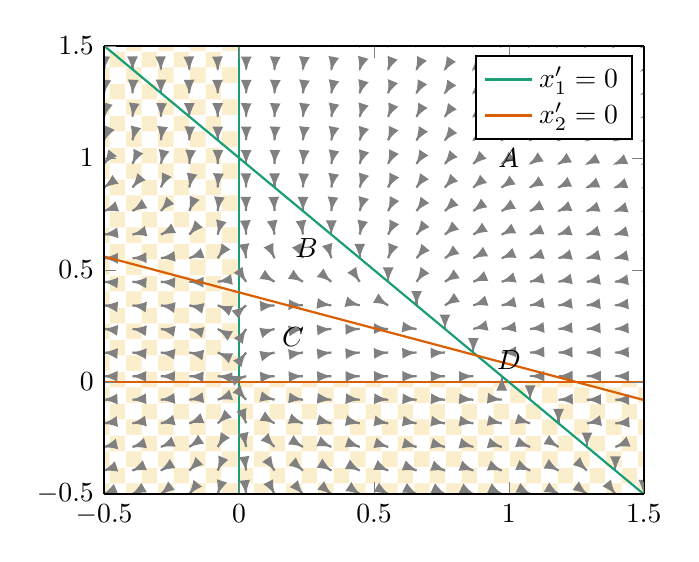
\begin{tikzpicture}
		\begin{axis}[
				view = {0}{90},
				xmin=-0.5, xmax=1.5, ymin=-0.5, ymax=1.5,
				domain=-0.5:1.5, y domain=-0.5:1.5,
				thick,
				]
				\draw[pattern=checkerboard, pattern color=Dark2-F, opacity=0.2] (0,0) -- (5,0) -- (5,-5) -- (-5,-5) -- (-5,5) -- (0,5) -- cycle;
				\addplot[Dark2-A] coordinates {(0,-5)(0,5)};
				\addplot[Dark2-B, samples=2] {0};

				\def\n{0.4}
				\addplot3 [gray, quiver={u={x * (1 - x) - x * y}, v={y * (\n - y) - 2 * pow(\n, 2) * x * y}, scale arrows=0.005, every arrow/.append style={-latex}}, samples=20] (x,y,0);

				\addplot[Dark2-A, samples=2] {1 - x};
				\addplot[Dark2-B, samples=2] {(\n - 2 * pow(\n, 2) * x)};
				\legend{$x_1'=0$, $x_2'=0$}

				\node at (1,1) {$A$};
				\node at (0.25,0.6) {$B$};
				\node at (0.2,0.2) {$C$};
				\node at (1,0.1) {$D$};
		\end{axis}
	\end{tikzpicture}
	\caption{Nullclines för systemet \eqref{eq:competition_model} tillsammas med riktingsfält för $\nu=2/5$. Områdena i första kvadranten som avgränsas av nullclinerna är namngivna. \label{fig:nullclines}}
\end{figure}

För att undersöka för vilka värden på $\nu$ som jämviktspunkten är \emph{stabil}
linjäriserar vi systemet i den punkten.
Jakobianen
$$ \left. Df = \begin{pmatrix}
	\frac{\partial f_1}{\partial x_1} & \frac{\partial f_1}{\partial x_2} \\
	\frac{\partial f_2}{\partial x_1} & \frac{\partial f_2}{\partial x_2}
\end{pmatrix} \right\lvert_{x^*} \eqqcolon A = \begin{pmatrix}
	-x_1 & -x_1 \\
	2\nu^2x_1 - 2\nu^2 & x_1 - 1
\end{pmatrix} $$
Därav då det karakteristiska polynomet ges av
$$ p(\lambda) = \lambda^2 - \lambda \trace A + \det A $$
med
$$ \trace A = -x_1 + x_1 - 1 = -1 < 0 \quad \det A = x_1 (x_1 - 1) (2\nu^2 - 1) \ne 0 $$
fås egenvärdena av
$$ \lambda_{1,2} = \frac{\trace A}2 \pm \sqrt{\left(\frac{\trace A}2\right)^2 - \det A} $$
Stabil omm $\Re(\lambda) \le 0 \, \forall \lambda \in \sigma(A)$
och alla egenvärden $\lambda$ med $\Re(\lambda) = 0$ är \emph{semisimple}
(algebraiska multipliciteten är lika med geometriska multipliciteten).
Då $\trace A < 0$ räcker det att $\det A > 0 \Leftrightarrow \nu < \frac1{\sqrt2}$
för att alla egenvärden ska ha negativ realdel,
Därför är $x^*$ stabil jämviktspunkt för \eqref{eq:competition_model}
endast då $\nu \in (0, \frac12)$ enligt Grobman-Hartman,
se figur~\ref{fig:phase_portrait1} där det tydligt syns
hur, i fallet då $x^*$ är stabil, lösningar graviterar mot $x^*$,
annars mot jämviktspunkterna på koordinataxlarna.
Ökning av $\nu$ innebär samtidigt en ökning av tillväxthastigheten
och maxkapaciteten av populationen $x_2$ och hastigheten
med vilken den minskar proportionellt med $x_1$.
Därför är det också logistkt att systemet blir ber labilt
i och med att $\nu$ blir större,
då alla de ovannämnda faktorerna hjälper till att svänga systemet
så att endast en art dominerar.

\begin{figure}
	\centering
	\renewcommand{\figurescale}{0.2}
	\subfloat[]{% This file was created by matlab2tikz.
%
%The latest updates can be retrieved from
%  http://www.mathworks.com/matlabcentral/fileexchange/22022-matlab2tikz-matlab2tikz
%where you can also make suggestions and rate matlab2tikz.
%
\definecolor{mycolor1}{rgb}{0.00000,0.44700,0.74100}%
\definecolor{mycolor2}{rgb}{0.85000,0.32500,0.09800}%
%
\begin{tikzpicture}

\begin{axis}[%
width=7.879in,
height=8.464in,
at={(1.322in,1.142in)},
scale only axis,
xmin=0,
xmax=1.5,
xlabel style={font=\color{white!15!black}},
xlabel={$\text{x}_\text{1}$},
ymin=0,
ymax=1.5,
ylabel style={font=\color{white!15!black}},
ylabel={$\text{x}_\text{2}$},
axis background/.style={fill=white},
axis x line*=bottom,
axis y line*=left,
legend style={legend cell align=left, align=left, draw=white!15!black},
scale=\figurescale
]
\addplot [color=mycolor1]
  table[row sep=crcr]{%
0	1\\
0.0808080808080808	0.919191919191919\\
0.161616161616162	0.838383838383838\\
0.242424242424242	0.757575757575758\\
0.323232323232323	0.676767676767677\\
0.404040404040404	0.595959595959596\\
0.484848484848485	0.515151515151515\\
0.565656565656566	0.434343434343434\\
0.646464646464647	0.353535353535353\\
0.727272727272727	0.272727272727273\\
0.808080808080808	0.191919191919192\\
0.888888888888889	0.111111111111111\\
0.96969696969697	0.0303030303030303\\
1.05050505050505	-0.0505050505050506\\
1.13131313131313	-0.131313131313131\\
1.21212121212121	-0.212121212121212\\
1.29292929292929	-0.292929292929293\\
1.37373737373737	-0.373737373737374\\
1.45454545454545	-0.454545454545455\\
1.53535353535354	-0.535353535353535\\
1.61616161616162	-0.616161616161616\\
1.6969696969697	-0.696969696969697\\
1.77777777777778	-0.777777777777778\\
1.85858585858586	-0.858585858585859\\
1.93939393939394	-0.939393939393939\\
2.02020202020202	-1.02020202020202\\
2.1010101010101	-1.1010101010101\\
2.18181818181818	-1.18181818181818\\
2.26262626262626	-1.26262626262626\\
2.34343434343434	-1.34343434343434\\
2.42424242424242	-1.42424242424242\\
2.50505050505051	-1.50505050505051\\
2.58585858585859	-1.58585858585859\\
2.66666666666667	-1.66666666666667\\
2.74747474747475	-1.74747474747475\\
2.82828282828283	-1.82828282828283\\
2.90909090909091	-1.90909090909091\\
2.98989898989899	-1.98989898989899\\
3.07070707070707	-2.07070707070707\\
3.15151515151515	-2.15151515151515\\
3.23232323232323	-2.23232323232323\\
3.31313131313131	-2.31313131313131\\
3.39393939393939	-2.39393939393939\\
3.47474747474747	-2.47474747474747\\
3.55555555555556	-2.55555555555556\\
3.63636363636364	-2.63636363636364\\
3.71717171717172	-2.71717171717172\\
3.7979797979798	-2.7979797979798\\
3.87878787878788	-2.87878787878788\\
3.95959595959596	-2.95959595959596\\
4.04040404040404	-3.04040404040404\\
4.12121212121212	-3.12121212121212\\
4.2020202020202	-3.2020202020202\\
4.28282828282828	-3.28282828282828\\
4.36363636363636	-3.36363636363636\\
4.44444444444444	-3.44444444444444\\
4.52525252525253	-3.52525252525253\\
4.60606060606061	-3.60606060606061\\
4.68686868686869	-3.68686868686869\\
4.76767676767677	-3.76767676767677\\
4.84848484848485	-3.84848484848485\\
4.92929292929293	-3.92929292929293\\
5.01010101010101	-4.01010101010101\\
5.09090909090909	-4.09090909090909\\
5.17171717171717	-4.17171717171717\\
5.25252525252525	-4.25252525252525\\
5.33333333333333	-4.33333333333333\\
5.41414141414141	-4.41414141414141\\
5.49494949494949	-4.49494949494949\\
5.57575757575758	-4.57575757575758\\
5.65656565656566	-4.65656565656566\\
5.73737373737374	-4.73737373737374\\
5.81818181818182	-4.81818181818182\\
5.8989898989899	-4.8989898989899\\
5.97979797979798	-4.97979797979798\\
6.06060606060606	-5.06060606060606\\
6.14141414141414	-5.14141414141414\\
6.22222222222222	-5.22222222222222\\
6.3030303030303	-5.3030303030303\\
6.38383838383838	-5.38383838383838\\
6.46464646464646	-5.46464646464646\\
6.54545454545455	-5.54545454545455\\
6.62626262626263	-5.62626262626263\\
6.70707070707071	-5.70707070707071\\
6.78787878787879	-5.78787878787879\\
6.86868686868687	-5.86868686868687\\
6.94949494949495	-5.94949494949495\\
7.03030303030303	-6.03030303030303\\
7.11111111111111	-6.11111111111111\\
7.19191919191919	-6.19191919191919\\
7.27272727272727	-6.27272727272727\\
7.35353535353535	-6.35353535353535\\
7.43434343434343	-6.43434343434343\\
7.51515151515152	-6.51515151515152\\
7.5959595959596	-6.5959595959596\\
7.67676767676768	-6.67676767676768\\
7.75757575757576	-6.75757575757576\\
7.83838383838384	-6.83838383838384\\
7.91919191919192	-6.91919191919192\\
8	-7\\
};

\addplot [color=mycolor2]
  table[row sep=crcr]{%
0	0.25\\
0.0808080808080808	0.23989898989899\\
0.161616161616162	0.22979797979798\\
0.242424242424242	0.21969696969697\\
0.323232323232323	0.20959595959596\\
0.404040404040404	0.19949494949495\\
0.484848484848485	0.189393939393939\\
0.565656565656566	0.179292929292929\\
0.646464646464647	0.169191919191919\\
0.727272727272727	0.159090909090909\\
0.808080808080808	0.148989898989899\\
0.888888888888889	0.138888888888889\\
0.96969696969697	0.128787878787879\\
1.05050505050505	0.118686868686869\\
1.13131313131313	0.108585858585859\\
1.21212121212121	0.0984848484848485\\
1.29292929292929	0.0883838383838384\\
1.37373737373737	0.0782828282828283\\
1.45454545454545	0.0681818181818182\\
1.53535353535354	0.0580808080808081\\
1.61616161616162	0.047979797979798\\
1.6969696969697	0.0378787878787879\\
1.77777777777778	0.0277777777777778\\
1.85858585858586	0.0176767676767677\\
1.93939393939394	0.00757575757575757\\
2.02020202020202	-0.00252525252525254\\
2.1010101010101	-0.0126262626262627\\
2.18181818181818	-0.0227272727272727\\
2.26262626262626	-0.0328282828282828\\
2.34343434343434	-0.0429292929292929\\
2.42424242424242	-0.053030303030303\\
2.50505050505051	-0.0631313131313131\\
2.58585858585859	-0.0732323232323233\\
2.66666666666667	-0.0833333333333333\\
2.74747474747475	-0.0934343434343434\\
2.82828282828283	-0.103535353535354\\
2.90909090909091	-0.113636363636364\\
2.98989898989899	-0.123737373737374\\
3.07070707070707	-0.133838383838384\\
3.15151515151515	-0.143939393939394\\
3.23232323232323	-0.154040404040404\\
3.31313131313131	-0.164141414141414\\
3.39393939393939	-0.174242424242424\\
3.47474747474747	-0.184343434343434\\
3.55555555555556	-0.194444444444444\\
3.63636363636364	-0.204545454545455\\
3.71717171717172	-0.214646464646465\\
3.7979797979798	-0.224747474747475\\
3.87878787878788	-0.234848484848485\\
3.95959595959596	-0.244949494949495\\
4.04040404040404	-0.255050505050505\\
4.12121212121212	-0.265151515151515\\
4.2020202020202	-0.275252525252525\\
4.28282828282828	-0.285353535353535\\
4.36363636363636	-0.295454545454545\\
4.44444444444444	-0.305555555555556\\
4.52525252525253	-0.315656565656566\\
4.60606060606061	-0.325757575757576\\
4.68686868686869	-0.335858585858586\\
4.76767676767677	-0.345959595959596\\
4.84848484848485	-0.356060606060606\\
4.92929292929293	-0.366161616161616\\
5.01010101010101	-0.376262626262626\\
5.09090909090909	-0.386363636363636\\
5.17171717171717	-0.396464646464647\\
5.25252525252525	-0.406565656565657\\
5.33333333333333	-0.416666666666667\\
5.41414141414141	-0.426767676767677\\
5.49494949494949	-0.436868686868687\\
5.57575757575758	-0.446969696969697\\
5.65656565656566	-0.457070707070707\\
5.73737373737374	-0.467171717171717\\
5.81818181818182	-0.477272727272727\\
5.8989898989899	-0.487373737373737\\
5.97979797979798	-0.497474747474748\\
6.06060606060606	-0.507575757575758\\
6.14141414141414	-0.517676767676768\\
6.22222222222222	-0.527777777777778\\
6.3030303030303	-0.537878787878788\\
6.38383838383838	-0.547979797979798\\
6.46464646464646	-0.558080808080808\\
6.54545454545455	-0.568181818181818\\
6.62626262626263	-0.578282828282828\\
6.70707070707071	-0.588383838383838\\
6.78787878787879	-0.598484848484849\\
6.86868686868687	-0.608585858585859\\
6.94949494949495	-0.618686868686869\\
7.03030303030303	-0.628787878787879\\
7.11111111111111	-0.638888888888889\\
7.19191919191919	-0.648989898989899\\
7.27272727272727	-0.659090909090909\\
7.35353535353535	-0.669191919191919\\
7.43434343434343	-0.679292929292929\\
7.51515151515152	-0.689393939393939\\
7.5959595959596	-0.69949494949495\\
7.67676767676768	-0.70959595959596\\
7.75757575757576	-0.71969696969697\\
7.83838383838384	-0.72979797979798\\
7.91919191919192	-0.73989898989899\\
8	-0.75\\
};

\addplot [color=blue]
  table[row sep=crcr]{%
0.252976190476191	1.38269704433498\\
0.246522078211571	1.31686837825883\\
0.240944494679873	1.25760684304243\\
0.236120598245465	1.20397748299331\\
0.231948633236797	1.15520404436924\\
0.223818447328069	1.0502440780471\\
0.218395360125684	0.964979945962969\\
0.215073745571136	0.894571132842364\\
0.213326990453037	0.835038337766732\\
0.212866231193309	0.771821773807125\\
0.214082102399327	0.719082717091197\\
0.216698500101744	0.674471357708201\\
0.220478776086685	0.636116283668928\\
0.227357173752945	0.590905234014418\\
0.235952287638944	0.55315489783205\\
0.246076462991809	0.521190222288469\\
0.257541695907551	0.493670408784679\\
0.27470902598101	0.462262589062711\\
0.293823771817789	0.435793213479662\\
0.31465985101269	0.413173697727359\\
0.336926479461361	0.393528563052865\\
0.36755424047103	0.371425884629682\\
0.399548517456582	0.352489614030102\\
0.43229085624214	0.336046664129867\\
0.465063022479705	0.321553681515468\\
0.504632441460857	0.305755178731414\\
0.542303230548035	0.291917916785314\\
0.577373958671501	0.279683362575064\\
0.609267745649631	0.268760152827424\\
0.642750105222013	0.257188809032064\\
0.671504768128239	0.246951292623471\\
0.695814375205112	0.23784765418042\\
0.716217261235017	0.22972095045213\\
0.734283305676654	0.222088944370445\\
0.749261033735342	0.215273729297492\\
0.761562660977786	0.209162988445276\\
0.771865617485184	0.203676556116167\\
0.780770610229783	0.198746998746021\\
0.788350155374764	0.194297526738377\\
0.794781878388992	0.190268662023339\\
0.800368165695209	0.186615071008913\\
0.806549620527419	0.182522481579731\\
0.811814479594001	0.178876915130394\\
0.816237024026709	0.175616199256521\\
0.820107565376551	0.172695028395922\\
0.824358019929648	0.169576691636252\\
0.827986371620792	0.166825157615363\\
0.831004336305723	0.164386966965619\\
0.833661228875193	0.162223699302573\\
0.836756074181888	0.159889303274054\\
0.839333639731764	0.157859353869073\\
0.841329238950123	0.156084984077809\\
0.843097341641885	0.154535616011371\\
0.845338791914997	0.153011513044784\\
0.847055108408394	0.151693207121805\\
0.847970894958801	0.150540939754225\\
0.848879198120755	0.149547001910423\\
0.850644514675649	0.148734811008399\\
0.851765354073779	0.148016217363033\\
0.851670337048445	0.147362352952869\\
0.851806958602735	0.146796675425594\\
0.853065213435735	0.146399572705601\\
0.853812431716814	0.146035635361464\\
0.853687568214337	0.1456909797925\\
0.853676541510773	0.145385598762499\\
0.854356636694399	0.145154513961067\\
0.854790274943746	0.144941128763949\\
0.854863016217028	0.144740319586259\\
0.85494838797397	0.144559217072073\\
0.855362396624449	0.144389407246495\\
0.855631190128961	0.144234637820326\\
0.855663816980032	0.144090745632501\\
0.855718612782746	0.143962313624697\\
0.856141802540852	0.143836248393646\\
0.85636801634118	0.143721782618727\\
0.856199305882651	0.143612132927312\\
0.856128184513317	0.143517541276602\\
0.856876029357842	0.143449532563493\\
0.857165419846005	0.143381241322979\\
0.856454892668282	0.14329828586373\\
0.856059724621097	0.143231325275368\\
0.856262440422968	0.143217916383955\\
0.856411727883661	0.143204045305525\\
0.856519488133598	0.14318996434013\\
0.856600546597639	0.1431759989766\\
};

\addplot [color=blue]
  table[row sep=crcr]{%
1.38392857142857	1.04649014778325\\
1.31846035383271	1.01222171824857\\
1.26028381039898	0.980477245688084\\
1.20830885538886	0.95098020636424\\
1.16163744876477	0.923492125330902\\
1.06308176313887	0.862001826474504\\
0.985677818740115	0.809476846226012\\
0.924011832761919	0.76408412364207\\
0.873590064002983	0.724363079942742\\
0.820800302736793	0.679909293691539\\
0.779086496614818	0.641634694185134\\
0.745831647298836	0.60833235021373\\
0.718916580885834	0.579039718312518\\
0.689044458532297	0.543173325694117\\
0.66678961293414	0.51253637151817\\
0.65037189566969	0.486066171823049\\
0.638284618618802	0.462913727695545\\
0.627215713340422	0.436226739772121\\
0.620796835254391	0.41336328153898\\
0.617963295789879	0.393555994302619\\
0.617749325332543	0.376187915923079\\
0.620236397700439	0.35674734201113\\
0.625212795320858	0.339957321439423\\
0.632023771488428	0.325305739597534\\
0.640007526888349	0.312376419074501\\
0.65086178759562	0.298208542881343\\
0.662382724977711	0.285842879810924\\
0.674194722806473	0.274954020842034\\
0.685867679423807	0.265273189348309\\
0.699522788447845	0.254774930178209\\
0.712439368596018	0.245535002249594\\
0.72453274789192	0.237345777259022\\
0.735648342725465	0.230032671992105\\
0.748153124287232	0.22187525934863\\
0.759226586899721	0.214705756258846\\
0.769014084151042	0.208367405789889\\
0.777619042182321	0.202729669682534\\
0.789148663215074	0.195169193619\\
0.798558887876866	0.188760990119048\\
0.805939102819698	0.183277680998012\\
0.812159831064674	0.178561849904793\\
0.817749535871329	0.174616112209787\\
0.822429945362778	0.171168309240525\\
0.826193843526234	0.168138351993568\\
0.829476515264758	0.16547249215986\\
0.832911634756258	0.162924937858175\\
0.835795563161255	0.160691680354475\\
0.838083453808421	0.158724483098754\\
0.840106542719212	0.156992492265612\\
0.842490575146677	0.155257491753628\\
0.844419139815903	0.153746981816721\\
0.845753715599466	0.152423303110753\\
0.846972053690244	0.151269709556578\\
0.848744138996727	0.150212523670101\\
0.850013797193308	0.149288400544559\\
0.850421153909959	0.148467912885937\\
0.850919743530279	0.147757516532432\\
0.852334008965022	0.147204234169301\\
0.853193392222891	0.146707241959203\\
0.853019199687445	0.146246136850544\\
0.853033773589973	0.145843714781917\\
0.853982527386964	0.145553538813384\\
0.854549808913704	0.145286209930934\\
0.854492392299373	0.145032394236126\\
0.854502574927932	0.14480617336273\\
0.855042236805386	0.144622281542172\\
0.85538019259154	0.144452910561007\\
0.855406051753073	0.144293416038719\\
0.85545426488626	0.144150261020003\\
0.855846391062195	0.144015191098266\\
0.856079245089132	0.1438920067163\\
0.856027117868664	0.143775917065867\\
0.856021862298535	0.143673476950155\\
0.856505684111555	0.143582847351069\\
0.85672846940859	0.143498334757468\\
0.856406969022402	0.143411567347429\\
0.856237397511896	0.143338123180694\\
0.857028212473567	0.143296989886697\\
0.857328866484936	0.143251179428678\\
0.856588783927333	0.143186627209443\\
0.856151840089991	0.14313509334281\\
0.856219041507885	0.143132499736824\\
0.856280172863601	0.143129817370243\\
0.856335808368302	0.14312705944535\\
0.856386475419873	0.143124238027545\\
};

\addplot [color=blue]
  table[row sep=crcr]{%
1.35615079365079	0.0193965517241383\\
1.29502533594902	0.0195657008566769\\
1.24586718350566	0.0197540394823484\\
1.20592635114125	0.0199586825343407\\
1.17286950765867	0.0201771269902951\\
1.13697619171067	0.0204851921544311\\
1.1084822510003	0.0208116385589657\\
1.08572055850772	0.0211542423714469\\
1.06721974555528	0.021510958208635\\
1.04767616015286	0.0219989518192497\\
1.03256715378576	0.0225067760273814\\
1.02088040793403	0.0230328118615943\\
1.01164677706402	0.0235753793904835\\
1.00235385333592	0.0242891037060669\\
0.995358395249735	0.0250266301745689\\
0.99012138788849	0.0257870296074692\\
0.986048103511573	0.0265690425239994\\
0.981923502038654	0.0275829019405027\\
0.978781684933401	0.0286293079639914\\
0.976394631102781	0.0297078834763928\\
0.974419240480661	0.0308176354100184\\
0.972127919252154	0.0322721121696102\\
0.970152774759315	0.033775777948955\\
0.968440260256596	0.0353281962882767\\
0.966793875001805	0.0369279754922428\\
0.964514691116309	0.0391013240237947\\
0.962275509676408	0.0413526225580322\\
0.960097815060679	0.0436790610019025\\
0.95785322783511	0.0460762078661209\\
0.954507928475123	0.049485747183745\\
0.951103991508397	0.0530081322616605\\
0.947702356159014	0.0566282368021475\\
0.944178514033623	0.0603274007300415\\
0.938912877840209	0.0655206958302592\\
0.933697805330037	0.0707747630092565\\
0.9287516824889	0.0760352307755054\\
0.92368237825774	0.0812406205939837\\
0.919095138978796	0.0854338086033184\\
0.914808943737462	0.089528860245996\\
0.911075939807936	0.0935042886044329\\
0.907332740219359	0.0973299913423807\\
0.903043411055264	0.100978805663664\\
0.899229617659372	0.104452594520913\\
0.896216024719288	0.107746685754908\\
0.893211701525249	0.110840878030185\\
0.889638483300349	0.113629431841798\\
0.88661425763318	0.116237345249798\\
0.88447880953515	0.118673743240613\\
0.882345763965017	0.120926067290962\\
0.879696775199146	0.122870808625807\\
0.877508968541862	0.124672934000667\\
0.876019339224699	0.126344441350615\\
0.87455702034385	0.127878996698312\\
0.872642656033885	0.129257959871321\\
0.87107319033067	0.13052523597605\\
0.87000779065804	0.131692111741251\\
0.868977182487959	0.132756085743092\\
0.867511299053635	0.133769837617572\\
0.866346516502592	0.134690945060534\\
0.865647652168655	0.135531360770805\\
0.864953482804088	0.136288481848282\\
0.863742918998006	0.137001431656726\\
0.862869161675555	0.137643805345884\\
0.86258271694182	0.138229104330224\\
0.862226576771382	0.138749150486699\\
0.861166313344488	0.139194349230932\\
0.860509412276112	0.139597904874579\\
0.860603997059756	0.139973449014762\\
0.860553622719298	0.140304603094508\\
0.860198115200623	0.140458260999776\\
0.859920227550406	0.140603929347734\\
0.859709889579224	0.140741950819069\\
0.859530338185938	0.140872003383276\\
};

\addplot [color=blue]
  table[row sep=crcr]{%
0.0863095238095238	0.052647783251232\\
0.0907431111267733	0.0532222440735314\\
0.0953760173834316	0.0537993870338497\\
0.100214378463511	0.0543790753457883\\
0.105264245078513	0.0549611652718581\\
0.132224398083779	0.0577467700624126\\
0.16463858195426	0.0605643805155806\\
0.202859749381226	0.0633925453886852\\
0.246905068739926	0.0662069597702475\\
0.313846450031611	0.0698820748686997\\
0.388047457975051	0.0734228027081451\\
0.465931720869672	0.0767745352718364\\
0.543143184607162	0.0798982190375803\\
0.629442951451515	0.0833509092568085\\
0.702948145254883	0.0864414064040493\\
0.761360227641327	0.0892017103177874\\
0.805025477011996	0.0916801976744434\\
0.826297873999528	0.0931419511146895\\
0.843219700110793	0.0945246201471214\\
0.856442601414702	0.0958387195801491\\
0.866651442327562	0.0970951048647998\\
0.874492008620885	0.0983033195461375\\
0.880390019498389	0.0994686954058089\\
0.884719015279169	0.100596147723867\\
0.887844352274244	0.101690754436615\\
0.890883472940891	0.103217556743099\\
0.892528302545268	0.104690241347143\\
0.893090610492739	0.106112235564977\\
0.893026607448023	0.107490247848251\\
0.892617778312968	0.109023431294235\\
0.891824945524391	0.110504016524168\\
0.890728456126743	0.111932755478238\\
0.889515676544863	0.113312674987274\\
0.887961697518742	0.115062834633301\\
0.886338165059215	0.116730553989932\\
0.884634500342944	0.118316371940036\\
0.882986558905196	0.119824058495095\\
0.881027248609001	0.12172990234902\\
0.879130751287138	0.123501741214251\\
0.877235860600253	0.125143462779082\\
0.875490774936669	0.126663851122696\\
0.873715977956504	0.128494248732615\\
0.871959808653224	0.130135201326603\\
0.869976934402576	0.131595874798757\\
0.868303552229016	0.132902707335292\\
0.86789490641445	0.134143105582028\\
0.866956211703365	0.13522715050426\\
0.864588621007429	0.136149033564179\\
0.862907368728325	0.136970399329918\\
0.863017169340196	0.137467322325303\\
0.862831246667045	0.137918252938249\\
0.862234619546692	0.138323328765589\\
0.861681591303186	0.138695847573043\\
0.861462577450683	0.139045135523223\\
0.861183950354143	0.139364317945192\\
0.860814359701122	0.139654844294533\\
0.860473718809353	0.139921607778184\\
0.860222431242853	0.140253943233803\\
0.859928810272346	0.140547911905836\\
0.859500093723019	0.140805260099697\\
0.859151753579697	0.141034760136425\\
0.859404514867744	0.141298747006237\\
0.859301701427282	0.141518974658663\\
0.85831353944424	0.141687469648097\\
0.857714397200501	0.141838921331515\\
0.858070296258649	0.141941459122458\\
0.858184181531019	0.142029644129021\\
0.857930755793705	0.14210122691729\\
0.8577183433895	0.142166768336765\\
0.857816905495953	0.142233412686383\\
0.857828689727375	0.142292117651488\\
0.857707831602323	0.142342299635608\\
0.857604687100167	0.142388078724745\\
0.857666021534942	0.142442407806561\\
0.857657146518369	0.142489235711427\\
0.857503275574592	0.14252738334636\\
0.857391887399081	0.142561960000577\\
};

\addplot [color=blue]
  table[row sep=crcr]{%
1.4156746031746	0.499692118226601\\
1.3492317283318	0.48839377464175\\
1.29109263015921	0.477841245067931\\
1.23987694798129	0.46795461142076\\
1.1944658936819	0.458665061162429\\
1.11212623736504	0.44037027683281\\
1.04688102380668	0.424136990741637\\
0.994531306931729	0.409612244087214\\
0.95157350841037	0.396507653749032\\
0.906208992772067	0.381259883611181\\
0.870407200439024	0.367700377926292\\
0.84197279197294	0.355550158140619\\
0.819084284534614	0.344579880765268\\
0.794410623219974	0.33108531790741\\
0.776129931795108	0.31916035577237\\
0.762772458788182	0.308536553068274\\
0.753043448199584	0.298992140113345\\
0.744377624910903	0.287937854082497\\
0.739342320851005	0.278154904541111\\
0.737069955614419	0.269429419560465\\
0.736722701998414	0.261582289214513\\
0.738085406632322	0.252794051932342\\
0.741032096649088	0.244978157489892\\
0.745099707025572	0.237979753184617\\
0.749771823053166	0.231666278457202\\
0.755783675321214	0.224706347968917\\
0.762005066686362	0.218492437043289\\
0.768268912670768	0.212914618543733\\
0.774312576477879	0.207876374579027\\
0.781261297118721	0.202253871052483\\
0.787708038979295	0.197246559808905\\
0.793680941377919	0.192767543464383\\
0.799103728696497	0.188740037754039\\
0.805442870832802	0.183981807083502\\
0.810996619379982	0.17980981009909\\
0.815871190251	0.176135089762641\\
0.8201432243507	0.172882781028816\\
0.827266803339247	0.167942317688287\\
0.832601314732723	0.163904644248551\\
0.835577514752889	0.160557053173992\\
0.838341246888271	0.157792498230378\\
0.840653808631898	0.15639802510504\\
0.842487755745188	0.155138086226912\\
0.843765674874122	0.153994118626069\\
0.84490582139213	0.152962836690539\\
0.846184027065593	0.152038875402134\\
0.847269295223002	0.151202380363315\\
0.848145601086869	0.150443271546788\\
0.84893586782682	0.149756111105567\\
0.850073671030615	0.148917520412859\\
0.850993982521956	0.148182966278603\\
0.85161505467418	0.147535902903111\\
0.852193864284474	0.146970063853948\\
0.853504929591193	0.146393614703259\\
0.854266860831443	0.145892874790542\\
0.853901325733921	0.145440369426697\\
0.853869594661666	0.145060462138697\\
0.854600872651287	0.144870207012617\\
0.855046666926484	0.144692081191327\\
0.8550928895292	0.1445215116329\\
0.855145873966363	0.144366912291668\\
0.855471799657267	0.144233348244895\\
0.855694759199517	0.144110212671133\\
0.855777942708963	0.143995409521265\\
0.855857434625105	0.143891186209413\\
0.85615355524652	0.143771627331006\\
0.856331642744563	0.143664356123011\\
0.856281868744627	0.143564884772101\\
0.856281011696012	0.143478336707509\\
0.857032053608819	0.143407112350361\\
0.857298485624462	0.143336617933085\\
0.856459854399455	0.143250191475051\\
0.856033604092697	0.143183047994934\\
0.856925705261577	0.143167681093821\\
0.857297598772287	0.143143500206879\\
0.856708395603795	0.143099564988254\\
0.856312117417653	0.143063506941873\\
};

\addplot [color=blue]
  table[row sep=crcr]{%
0.856150793650794	1.4362684729064\\
0.815974560255256	1.36787334418867\\
0.780795709988222	1.30627077997725\\
0.749805840856221	1.2504936776292\\
0.722347790382752	1.19973928355534\\
0.669570600610409	1.09810576042779\\
0.628633251982587	1.01415522142504\\
0.596544444603323	0.943760007393533\\
0.570796575326997	0.883604165929533\\
0.544621958513916	0.818028213316588\\
0.524704550736969	0.762898092624856\\
0.509612452242872	0.715939906433817\\
0.498169553095958	0.675348546558602\\
0.486846164244336	0.627030926403586\\
0.479921753301645	0.586482624105361\\
0.476435440822882	0.551997379268648\\
0.475551770054456	0.5222142372113\\
0.477421118857703	0.488485106984411\\
0.482156066750507	0.459943893282873\\
0.489142610734973	0.435485433620708\\
0.49779266816188	0.414224909187257\\
0.510765844719849	0.390420787799325\\
0.525291885738015	0.370062410904743\\
0.540886668203953	0.352444668661775\\
0.557029267286498	0.336998601147654\\
0.577439192746844	0.32005615851867\\
0.597673939275308	0.305367759400308\\
0.617378615534379	0.292505768073216\\
0.636158701492425	0.281120837677463\\
0.657474153286787	0.268837813034316\\
0.676967113956831	0.258070016282954\\
0.694625648217203	0.248560298777434\\
0.710420281022638	0.24009604294701\\
0.728354192197408	0.230387250278713\\
0.743658910736815	0.221925324905545\\
0.756640599161277	0.214500233121273\\
0.767708876071689	0.207946306117357\\
0.780615007251689	0.200247578552057\\
0.791040764396732	0.193651964493089\\
0.799055124914372	0.18794760942923\\
0.80578308776441	0.183001449335957\\
0.811432327179174	0.179127003514007\\
0.816253246673936	0.175685818578188\\
0.820300880348955	0.172616563758114\\
0.823850526371906	0.169874509774906\\
0.827806855753035	0.166932386027338\\
0.831169557944615	0.164347405506215\\
0.833934459584215	0.162066121660637\\
0.836367942327591	0.16005085938148\\
0.839221876313593	0.15791758876322\\
0.841568057153832	0.156067783593191\\
0.843306185779567	0.154454439824721\\
0.844860152163078	0.153050992273082\\
0.846945086735489	0.151726680711049\\
0.848480434714295	0.150577715289756\\
0.849109651420261	0.14956728470466\\
0.849802743603336	0.148696209284687\\
0.85145275332294	0.148017261204908\\
0.852465757795625	0.147410905240232\\
0.852279053546449	0.146851944469731\\
0.852319579598719	0.146366094943274\\
0.853414137851555	0.146025499129588\\
0.854074091070343	0.145711979378874\\
0.854028229815171	0.145414903954949\\
0.85405375540535	0.145149986451836\\
0.854636932943121	0.144938343568229\\
0.855014279452563	0.144743429491106\\
0.855088310836218	0.144560722389464\\
0.855173317827765	0.144396040241097\\
0.855569577420009	0.144236446318568\\
0.855820390558467	0.144091488372592\\
0.855820991982119	0.143956639427011\\
0.855854606062535	0.143837059297999\\
0.856327829444753	0.143724379043166\\
0.856559118582991	0.143621126978376\\
0.856287625269951	0.143519090852354\\
0.856155250097005	0.143432212927828\\
0.857003321529022	0.143378911788384\\
0.857322523702562	0.143321880702952\\
0.856496785044095	0.143245230468145\\
0.856022620597527	0.143184180421202\\
0.856192297211745	0.143176443180571\\
0.856327541197465	0.143168263952859\\
0.85643518177965	0.143159796338989\\
0.856521726429044	0.143151186423362\\
};

\addplot [color=blue]
  table[row sep=crcr]{%
0.0327380952380952	0.276169950738917\\
0.0344234625849265	0.275567044410321\\
0.0361926234651097	0.274973100327917\\
0.0380493228020317	0.274387678327552\\
0.0399974308931202	0.27381034131411\\
0.0500941465348175	0.271280491035289\\
0.0625642180739652	0.268868209548874\\
0.0778446619589532	0.266533825075212\\
0.0963862966941386	0.264237397769012\\
0.125469262941311	0.261298429649972\\
0.161385462744315	0.258273254557942\\
0.204454678099488	0.255085094434836\\
0.254284615680241	0.251670516114144\\
0.320810201072961	0.247253151066228\\
0.391684834166874	0.242427962853972\\
0.462610663962055	0.237232349607683\\
0.529377893860969	0.231761681859861\\
0.583053965027652	0.226713986874551\\
0.629320108880993	0.221657703548116\\
0.667833073042197	0.216681519570883\\
0.699123751342178	0.211866979341596\\
0.724425607145165	0.20728346281779\\
0.744537764408589	0.202947097051349\\
0.760247317878894	0.198864073201414\\
0.772677496127117	0.195053760543868\\
0.782428380866996	0.191684352511449\\
0.790397170310576	0.188546776731593\\
0.796896997537072	0.185625639078287\\
0.802344552371178	0.182911920826342\\
0.807932646408639	0.17993844630928\\
0.812605409414573	0.177213137830107\\
0.816491977067321	0.174710881170517\\
0.819863379636138	0.172414745926625\\
0.82361600556255	0.169845550042812\\
0.826835648213484	0.167526370430546\\
0.829556694136684	0.165427059017925\\
0.831970080921454	0.163526221171445\\
0.83486791060557	0.161334878153734\\
0.837343858007017	0.159396808400729\\
0.839385044899905	0.157676477992109\\
0.84119583204089	0.156149232045048\\
0.843474979802121	0.154451865343599\\
0.845325216787229	0.152982652916851\\
0.846625857775696	0.15170302459947\\
0.847808099656025	0.15059372541001\\
0.849698222564577	0.149559094916045\\
0.850964669152282	0.148661121275525\\
0.851071542498451	0.147863966297832\\
0.851398795595262	0.147182865640633\\
0.853115778906341	0.14670234601715\\
0.854039413851914	0.146264565029164\\
0.853412460116024	0.145843456821475\\
0.853127745340355	0.145479063643072\\
0.854148688513077	0.145248105229144\\
0.854743117482876	0.145030960743953\\
0.854704945642909	0.144820256019303\\
0.854701615386683	0.144630392786812\\
0.855152394388403	0.144474733885291\\
0.855446235749721	0.144330512024015\\
0.855524114890026	0.144194866189946\\
0.855600909867689	0.144071790047056\\
0.855918874333772	0.143942781019049\\
0.856118269359347	0.143825905192274\\
0.85610755141884	0.143717273292823\\
0.856128749980865	0.143621305066741\\
0.856628302216068	0.143530982633351\\
0.856845010577175	0.143447136287409\\
0.856445204088035	0.14335996119828\\
0.856243292966978	0.143287703094135\\
0.857277066742041	0.143256877281108\\
0.857644227155834	0.143216770038504\\
0.856557598703996	0.143147760566353\\
0.855923841901836	0.143095115284902\\
};

\addplot [color=blue]
  table[row sep=crcr]{%
0.939484126984127	1.12961822660099\\
0.895464520060556	1.07934771518462\\
0.857091937774053	1.03388856760081\\
0.823435435095698	0.992576872891407\\
0.793740524484793	0.954858782122041\\
0.737879621147371	0.880139006588554\\
0.69481417372526	0.817838274768209\\
0.661310317043161	0.765154374626023\\
0.634643595849058	0.71984795835023\\
0.607890899371457	0.670356237585217\\
0.587828828054362	0.628449434027783\\
0.572923858801821	0.592525874149396\\
0.561902175698542	0.561312418857029\\
0.551536161429923	0.5244254330356\\
0.545696413899434	0.493219823992263\\
0.54337450342683	0.466488139932353\\
0.543670851364812	0.443265369040927\\
0.546947448067783	0.417247366067108\\
0.552885974320358	0.395028518159595\\
0.560846343737582	0.375831312588475\\
0.570195042752258	0.359030107752515\\
0.583333163483301	0.340433345709403\\
0.597469311796391	0.324372225451139\\
0.612153026984856	0.310355267840005\\
0.626890048430725	0.297982396747607\\
0.644582888577088	0.284559974960734\\
0.661577761356785	0.272827580875107\\
0.67767948715057	0.262486458914675\\
0.69264462830395	0.253289426176221\\
0.709365971150756	0.2432417268142\\
0.724309667175225	0.234416712119438\\
0.737597142107709	0.226615155451222\\
0.749317050371539	0.21967182942804\\
0.763736212451167	0.211012534541652\\
0.775730782932915	0.203569864081017\\
0.785560116598013	0.197121174773837\\
0.793849836858782	0.191501589379692\\
0.801714177542552	0.186234428879528\\
0.808297381744643	0.181640949450553\\
0.813663740739744	0.177610008097485\\
0.818294974322637	0.174063614272943\\
0.822914247260545	0.170701392853952\\
0.826829617224513	0.167748227992632\\
0.830044988868676	0.165141963201864\\
0.83286613670755	0.162838969085529\\
0.83603538894906	0.16046376009358\\
0.838675002737897	0.158394643762925\\
0.840718455507832	0.156582761075055\\
0.842529743334205	0.154997906446377\\
0.844772918169782	0.153446724095782\\
0.84651687852976	0.152101413866724\\
0.847526275364219	0.150923800881392\\
0.848498434951792	0.149904271148633\\
0.850212803388387	0.149045766399974\\
0.851345541296816	0.148288343706801\\
0.851409178268271	0.147604307768414\\
0.851652221003339	0.147011471019228\\
0.852910647930953	0.146579193745335\\
0.853667281179795	0.146185488761433\\
0.853545740900707	0.145815343281726\\
0.853550697508686	0.14548857560376\\
0.854284107133204	0.145242174999958\\
0.854744450665121	0.145015069057197\\
0.854788554535283	0.144801144229656\\
0.854858053605584	0.144608960315414\\
0.855304816140169	0.144435667496536\\
0.855590156459541	0.144277355196296\\
0.855613342150255	0.14412959628425\\
0.855661751119616	0.143997666250087\\
0.856081004818975	0.14387077027474\\
0.856309821328592	0.143755293632834\\
0.856165975122978	0.143644921790026\\
0.856107270933432	0.143549133048318\\
0.856765066353633	0.143476327757531\\
0.857031611547016	0.143405024922123\\
0.856457051988604	0.143323024339061\\
0.85613749780883	0.143255703982115\\
0.856518152967822	0.143228753281526\\
0.856721985677661	0.143200587600056\\
0.856695093518472	0.143169636666439\\
0.856667553984046	0.143141276841891\\
};

\end{axis}
\end{tikzpicture}%
 \label{fig:mod1_stable}}
	\subfloat[]{% This file was created by matlab2tikz.
%
%The latest updates can be retrieved from
%  http://www.mathworks.com/matlabcentral/fileexchange/22022-matlab2tikz-matlab2tikz
%where you can also make suggestions and rate matlab2tikz.
%
\definecolor{mycolor1}{rgb}{0.00000,0.44700,0.74100}%
\definecolor{mycolor2}{rgb}{0.85000,0.32500,0.09800}%
%
\begin{tikzpicture}

\begin{axis}[%
width=7.879in,
height=8.464in,
at={(1.322in,1.142in)},
scale only axis,
xmin=0,
xmax=1.5,
xlabel style={font=\color{white!15!black}},
xlabel={$\text{x}_\text{1}$},
ymin=0,
ymax=1.5,
ylabel style={font=\color{white!15!black}},
ylabel={$\text{x}_\text{2}$},
axis background/.style={fill=white},
axis x line*=bottom,
axis y line*=left,
legend style={legend cell align=left, align=left, draw=white!15!black},
scale=\figurescale
]
\addplot [color=mycolor1]
  table[row sep=crcr]{%
0	1\\
0.0808080808080808	0.919191919191919\\
0.161616161616162	0.838383838383838\\
0.242424242424242	0.757575757575758\\
0.323232323232323	0.676767676767677\\
0.404040404040404	0.595959595959596\\
0.484848484848485	0.515151515151515\\
0.565656565656566	0.434343434343434\\
0.646464646464647	0.353535353535353\\
0.727272727272727	0.272727272727273\\
0.808080808080808	0.191919191919192\\
0.888888888888889	0.111111111111111\\
0.96969696969697	0.0303030303030303\\
1.05050505050505	-0.0505050505050506\\
1.13131313131313	-0.131313131313131\\
1.21212121212121	-0.212121212121212\\
1.29292929292929	-0.292929292929293\\
1.37373737373737	-0.373737373737374\\
1.45454545454545	-0.454545454545455\\
1.53535353535354	-0.535353535353535\\
1.61616161616162	-0.616161616161616\\
1.6969696969697	-0.696969696969697\\
1.77777777777778	-0.777777777777778\\
1.85858585858586	-0.858585858585859\\
1.93939393939394	-0.939393939393939\\
2.02020202020202	-1.02020202020202\\
2.1010101010101	-1.1010101010101\\
2.18181818181818	-1.18181818181818\\
2.26262626262626	-1.26262626262626\\
2.34343434343434	-1.34343434343434\\
2.42424242424242	-1.42424242424242\\
2.50505050505051	-1.50505050505051\\
2.58585858585859	-1.58585858585859\\
2.66666666666667	-1.66666666666667\\
2.74747474747475	-1.74747474747475\\
2.82828282828283	-1.82828282828283\\
2.90909090909091	-1.90909090909091\\
2.98989898989899	-1.98989898989899\\
3.07070707070707	-2.07070707070707\\
3.15151515151515	-2.15151515151515\\
3.23232323232323	-2.23232323232323\\
3.31313131313131	-2.31313131313131\\
3.39393939393939	-2.39393939393939\\
3.47474747474747	-2.47474747474747\\
3.55555555555556	-2.55555555555556\\
3.63636363636364	-2.63636363636364\\
3.71717171717172	-2.71717171717172\\
3.7979797979798	-2.7979797979798\\
3.87878787878788	-2.87878787878788\\
3.95959595959596	-2.95959595959596\\
4.04040404040404	-3.04040404040404\\
4.12121212121212	-3.12121212121212\\
4.2020202020202	-3.2020202020202\\
4.28282828282828	-3.28282828282828\\
4.36363636363636	-3.36363636363636\\
4.44444444444444	-3.44444444444444\\
4.52525252525253	-3.52525252525253\\
4.60606060606061	-3.60606060606061\\
4.68686868686869	-3.68686868686869\\
4.76767676767677	-3.76767676767677\\
4.84848484848485	-3.84848484848485\\
4.92929292929293	-3.92929292929293\\
5.01010101010101	-4.01010101010101\\
5.09090909090909	-4.09090909090909\\
5.17171717171717	-4.17171717171717\\
5.25252525252525	-4.25252525252525\\
5.33333333333333	-4.33333333333333\\
5.41414141414141	-4.41414141414141\\
5.49494949494949	-4.49494949494949\\
5.57575757575758	-4.57575757575758\\
5.65656565656566	-4.65656565656566\\
5.73737373737374	-4.73737373737374\\
5.81818181818182	-4.81818181818182\\
5.8989898989899	-4.8989898989899\\
5.97979797979798	-4.97979797979798\\
6.06060606060606	-5.06060606060606\\
6.14141414141414	-5.14141414141414\\
6.22222222222222	-5.22222222222222\\
6.3030303030303	-5.3030303030303\\
6.38383838383838	-5.38383838383838\\
6.46464646464646	-5.46464646464646\\
6.54545454545455	-5.54545454545455\\
6.62626262626263	-5.62626262626263\\
6.70707070707071	-5.70707070707071\\
6.78787878787879	-5.78787878787879\\
6.86868686868687	-5.86868686868687\\
6.94949494949495	-5.94949494949495\\
7.03030303030303	-6.03030303030303\\
7.11111111111111	-6.11111111111111\\
7.19191919191919	-6.19191919191919\\
7.27272727272727	-6.27272727272727\\
7.35353535353535	-6.35353535353535\\
7.43434343434343	-6.43434343434343\\
7.51515151515152	-6.51515151515152\\
7.5959595959596	-6.5959595959596\\
7.67676767676768	-6.67676767676768\\
7.75757575757576	-6.75757575757576\\
7.83838383838384	-6.83838383838384\\
7.91919191919192	-6.91919191919192\\
8	-7\\
};

\addplot [color=mycolor2]
  table[row sep=crcr]{%
0	1.25\\
0.0808080808080808	0.997474747474747\\
0.161616161616162	0.744949494949495\\
0.242424242424242	0.492424242424242\\
0.323232323232323	0.23989898989899\\
0.404040404040404	-0.0126262626262625\\
0.484848484848485	-0.265151515151515\\
0.565656565656566	-0.517676767676768\\
0.646464646464647	-0.77020202020202\\
0.727272727272727	-1.02272727272727\\
0.808080808080808	-1.27525252525253\\
0.888888888888889	-1.52777777777778\\
0.96969696969697	-1.78030303030303\\
1.05050505050505	-2.03282828282828\\
1.13131313131313	-2.28535353535354\\
1.21212121212121	-2.53787878787879\\
1.29292929292929	-2.79040404040404\\
1.37373737373737	-3.04292929292929\\
1.45454545454545	-3.29545454545455\\
1.53535353535354	-3.5479797979798\\
1.61616161616162	-3.80050505050505\\
1.6969696969697	-4.0530303030303\\
1.77777777777778	-4.30555555555556\\
1.85858585858586	-4.55808080808081\\
1.93939393939394	-4.81060606060606\\
2.02020202020202	-5.06313131313131\\
2.1010101010101	-5.31565656565657\\
2.18181818181818	-5.56818181818182\\
2.26262626262626	-5.82070707070707\\
2.34343434343434	-6.07323232323232\\
2.42424242424242	-6.32575757575758\\
2.50505050505051	-6.57828282828283\\
2.58585858585859	-6.83080808080808\\
2.66666666666667	-7.08333333333333\\
2.74747474747475	-7.33585858585858\\
2.82828282828283	-7.58838383838384\\
2.90909090909091	-7.84090909090909\\
2.98989898989899	-8.09343434343434\\
3.07070707070707	-8.3459595959596\\
3.15151515151515	-8.59848484848485\\
3.23232323232323	-8.8510101010101\\
3.31313131313131	-9.10353535353535\\
3.39393939393939	-9.35606060606061\\
3.47474747474747	-9.60858585858586\\
3.55555555555556	-9.86111111111111\\
3.63636363636364	-10.1136363636364\\
3.71717171717172	-10.3661616161616\\
3.7979797979798	-10.6186868686869\\
3.87878787878788	-10.8712121212121\\
3.95959595959596	-11.1237373737374\\
4.04040404040404	-11.3762626262626\\
4.12121212121212	-11.6287878787879\\
4.2020202020202	-11.8813131313131\\
4.28282828282828	-12.1338383838384\\
4.36363636363636	-12.3863636363636\\
4.44444444444444	-12.6388888888889\\
4.52525252525253	-12.8914141414141\\
4.60606060606061	-13.1439393939394\\
4.68686868686869	-13.3964646464646\\
4.76767676767677	-13.6489898989899\\
4.84848484848485	-13.9015151515152\\
4.92929292929293	-14.1540404040404\\
5.01010101010101	-14.4065656565657\\
5.09090909090909	-14.6590909090909\\
5.17171717171717	-14.9116161616162\\
5.25252525252525	-15.1641414141414\\
5.33333333333333	-15.4166666666667\\
5.41414141414141	-15.6691919191919\\
5.49494949494949	-15.9217171717172\\
5.57575757575758	-16.1742424242424\\
5.65656565656566	-16.4267676767677\\
5.73737373737374	-16.6792929292929\\
5.81818181818182	-16.9318181818182\\
5.8989898989899	-17.1843434343434\\
5.97979797979798	-17.4368686868687\\
6.06060606060606	-17.6893939393939\\
6.14141414141414	-17.9419191919192\\
6.22222222222222	-18.1944444444444\\
6.3030303030303	-18.4469696969697\\
6.38383838383838	-18.699494949495\\
6.46464646464646	-18.9520202020202\\
6.54545454545455	-19.2045454545455\\
6.62626262626263	-19.4570707070707\\
6.70707070707071	-19.709595959596\\
6.78787878787879	-19.9621212121212\\
6.86868686868687	-20.2146464646465\\
6.94949494949495	-20.4671717171717\\
7.03030303030303	-20.719696969697\\
7.11111111111111	-20.9722222222222\\
7.19191919191919	-21.2247474747475\\
7.27272727272727	-21.4772727272727\\
7.35353535353535	-21.729797979798\\
7.43434343434343	-21.9823232323232\\
7.51515151515152	-22.2348484848485\\
7.5959595959596	-22.4873737373737\\
7.67676767676768	-22.739898989899\\
7.75757575757576	-22.9924242424242\\
7.83838383838384	-23.2449494949495\\
7.91919191919192	-23.4974747474747\\
8	-23.75\\
};

\addplot [color=blue]
  table[row sep=crcr]{%
0.403769841269841	1.47690886699507\\
0.392492326675172	1.40707646790735\\
0.38251700824211	1.34504397549024\\
0.373654478715284	1.28958508507013\\
0.365747890943155	1.2396951968697\\
0.350764257072553	1.14344388889098\\
0.339004467155857	1.06526849512695\\
0.329744248213188	1.00073115323243\\
0.322377311097828	0.946121642412582\\
0.315093209022151	0.887057855624073\\
0.309799403216313	0.83774426600552\\
0.306105804694589	0.795916769099557\\
0.303686870257114	0.759708086943589\\
0.302032960043043	0.716774722712201\\
0.302031227501607	0.680160810222216\\
0.303413434256516	0.648318519448472\\
0.305945234162999	0.619921736002411\\
0.310746043067875	0.586384035788702\\
0.317089720149867	0.556103144636958\\
0.324845305818002	0.528142817694924\\
0.333887741608825	0.50165983255407\\
0.347088641355415	0.46927869637876\\
0.362247527667578	0.43779777553115\\
0.379378417154225	0.406780453790326\\
0.398460392727161	0.375815704586846\\
0.423876868393596	0.338447846114436\\
0.452204657266553	0.30104683965058\\
0.483464837490459	0.263939087018981\\
0.517466244365173	0.227431115323654\\
0.556139983375655	0.189827943772305\\
0.59716013591181	0.154567672215748\\
0.639882143558292	0.122631380610848\\
0.683160579870525	0.0944851695519266\\
0.710815829299927	0.0784374701007258\\
0.737927652445881	0.0642809863163542\\
0.764208843103766	0.052034149971008\\
0.789346262827173	0.0415983539415492\\
0.813047773013535	0.0328101211952875\\
0.835178408384242	0.0255780873802731\\
0.855632212146529	0.0197582284780703\\
0.87429105530637	0.0151187781437004\\
0.888169380928425	0.0120372202473461\\
0.900852371215886	0.00952813618521533\\
0.912379168816688	0.00751072553901874\\
0.922787917501989	0.0058944608084268\\
0.930860623774358	0.00476568957818366\\
0.938198964461923	0.00384170534907742\\
0.944849576679587	0.00309072923031814\\
0.950857308924658	0.00248106317461356\\
0.95587696888752	0.00201942182025985\\
0.960425675260014	0.00164087606028906\\
0.964539960713875	0.00133198263198494\\
0.968254295973655	0.00107989333535569\\
0.971460291296253	0.000882015523404398\\
0.97435952748837	0.000719651922920838\\
0.976978198756106	0.000586923326985751\\
0.979340746425891	0.000478327023976699\\
0.98141408496263	0.00039147732250125\\
0.983286507405734	0.000320192212551221\\
0.984976115967606	0.000261859891333533\\
0.986499688547799	0.000214064180089374\\
0.988051831437054	0.00016989877501238\\
0.989429448075676	0.000134775583747397\\
0.990651235385176	0.000106987977516482\\
0.991734252770594	8.49209500306935e-05\\
0.992828103144724	6.4913237758956e-05\\
0.993779089800964	4.95990708944647e-05\\
0.994605223273578	3.79994527995496e-05\\
0.995322730389607	2.91329858103412e-05\\
0.996049334158277	2.11318335113908e-05\\
0.996663843383471	1.53200359826121e-05\\
0.997182981385657	1.12084447144381e-05\\
0.997621707691972	8.23008489404057e-06\\
0.998064909149696	5.51974676408795e-06\\
0.998425761327481	3.69291122186803e-06\\
0.998718860421777	2.56144023518702e-06\\
0.998957391993224	1.80871398790577e-06\\
0.999197126860438	1.04973228583278e-06\\
0.999381787252376	5.94718389369016e-07\\
0.999522882458347	4.1179493796917e-07\\
0.999631515678713	3.15104521169925e-07\\
0.999740096194292	1.10623963804977e-07\\
0.999816796808156	1.09717967311919e-08\\
0.999868879225943	4.89026609169985e-08\\
0.999905510017506	8.48453189759834e-08\\
0.99994326896952	-6.54445669414186e-08\\
0.999966462165592	-1.17718534087843e-07\\
0.999977199031666	3.14714147981527e-08\\
0.999983286104103	1.2503836150033e-07\\
0.999991539830195	-5.18442311818863e-07\\
0.99999612542947	-6.93495294147548e-07\\
0.999997296632255	2.20769355338166e-07\\
0.999997484127792	7.06600094463893e-07\\
0.999997902689211	1.46433479011798e-07\\
0.999998338959156	-1.0503570440133e-07\\
0.999999046067344	1.0928300612079e-07\\
0.999999550846169	2.76925867130137e-07\\
0.999999543857063	5.73860598595916e-08\\
0.999999597938612	-4.11692007058217e-08\\
0.999999800410574	4.28292041682911e-08\\
0.999999947652215	1.08533680632738e-07\\
0.999999786591812	-9.52206316977704e-08\\
0.99999975054964	-1.64980945125624e-07\\
1.00000000849473	4.39914461788353e-08\\
1.00000016733701	1.73695300698387e-07\\
0.999999411917026	-5.00705874979602e-07\\
0.999999197883781	-6.95407475623128e-07\\
1.00000023025218	2.06635074664281e-07\\
1.00000080163364	7.06361633107994e-07\\
1.00000014549043	1.30653243153172e-07\\
0.999999854469601	-1.25066260790902e-07\\
1.00000012415901	1.1022689543899e-07\\
1.00000033194615	2.91576534762916e-07\\
1.00000006076167	5.3929269060591e-08\\
0.999999940403003	-5.16299669091219e-08\\
1.00000005158556	4.54987717771889e-08\\
1.00000013726214	1.20360231532324e-07\\
0.999999892362624	-9.40284603300244e-08\\
0.999999807380881	-1.68449774130875e-07\\
1.00000005146521	4.50941526792316e-08\\
1.00000020434806	1.78849269330295e-07\\
0.999999485201907	-4.50413827181165e-07\\
0.99999927308723	-6.36021383596792e-07\\
1.00000021105826	1.84684628033358e-07\\
1.00000073838257	6.46079796400901e-07\\
1.00000010503767	9.19081144007678e-08\\
0.999999829044776	-1.49581152515067e-07\\
1.00000011781718	1.03093607523668e-07\\
1.00000033511402	2.93225439116752e-07\\
1.00000004766727	4.17100307516344e-08\\
0.999999922406775	-6.78923456071395e-08\\
1.00000005347069	4.67881216157351e-08\\
1.00000015209427	1.33083000279195e-07\\
0.999999885813572	-9.99114653372233e-08\\
0.999999792953287	-1.81163567433653e-07\\
1.00000005553617	4.85947979797019e-08\\
1.00000022050896	1.9294445175847e-07\\
0.999999519160874	-4.20724054957855e-07\\
0.999999307604681	-6.05830760171587e-07\\
1.00000019660059	1.7202573697679e-07\\
1.0000007040321	6.16016143541217e-07\\
0.999999307758168	-6.05679602359825e-07\\
0.999998836423022	-1.01807384362353e-06\\
1.00000030991674	2.71186054602734e-07\\
1.00000121600411	1.06396924970582e-06\\
1.00000013729231	1.20118624766585e-07\\
0.999999672978825	-2.86137795530998e-07\\
1.00000019769787	1.72989901797614e-07\\
1.00000058705618	5.13670923948893e-07\\
1.00000015951864	1.39577595998822e-07\\
0.999999961055613	-3.40755748229741e-08\\
1.00000008964123	7.84371985891677e-08\\
1.00000019608573	1.71575570682705e-07\\
0.999999967699667	-2.82617014724975e-08\\
0.999999878058796	-1.06697054736611e-07\\
1.00000004090647	3.57939255942552e-08\\
1.00000015208909	1.33077891787272e-07\\
0.999999743273541	-2.24632109119888e-07\\
0.999999615123682	-3.36761527987596e-07\\
1.00000010575295	9.25342408350368e-08\\
1.00000039309018	3.43950245839131e-07\\
0.999999833176814	-1.45967273966524e-07\\
0.999999626401347	-3.26891537103222e-07\\
1.00000010645009	9.31459437544631e-08\\
1.00000041996961	3.67470004554302e-07\\
};

\addplot [color=blue]
  table[row sep=crcr]{%
0.189484126984127	1.48614532019704\\
0.182303600684577	1.41731245744897\\
0.176147420554492	1.35864112350645\\
0.170826355534116	1.30817884596314\\
0.166187430944278	1.26435760847182\\
0.159345785343739	1.19997398564017\\
0.153842856545971	1.14839382534717\\
0.149374019013746	1.1066076081713\\
0.145680862241196	1.07205475773548\\
0.141766144095873	1.0352885365869\\
0.138659446023234	1.00593085538647\\
0.13618461791006	0.982314144415683\\
0.134188563136075	0.962988543723383\\
0.13209594720324	0.942260642367543\\
0.130523092940303	0.926105117044124\\
0.129356108354613	0.913479793023217\\
0.128488361902913	0.903407853351173\\
0.12769531744142	0.893170897367145\\
0.127196707842515	0.885354971018291\\
0.1269293408374	0.879389688870069\\
0.126826115507292	0.874671194989106\\
0.12685549714635	0.869843840213233\\
0.127043032763844	0.866065305507848\\
0.127361429516809	0.863074017232944\\
0.127772139762342	0.860514089452741\\
0.128381259580852	0.857507792945045\\
0.129100246610739	0.854773119164414\\
0.129926351979223	0.852223317193157\\
0.130841714119967	0.849644760714056\\
0.132146880268364	0.846009817675525\\
0.133617855046009	0.842156086222931\\
0.13527573609018	0.838052509577689\\
0.137125958243557	0.833518780342442\\
0.139934667123675	0.826474996081219\\
0.143217528172325	0.818449755991549\\
0.147079403565314	0.809333497943254\\
0.1516082352958	0.798688632521439\\
0.158172061331902	0.782549015814142\\
0.166368936715373	0.763468718800571\\
0.176798297612718	0.741154218455533\\
0.189927330258247	0.713199472025231\\
0.199946575582063	0.691381923519873\\
0.211809395101623	0.666603035077329\\
0.225969979809469	0.638463708383914\\
0.242885520917614	0.60602200377913\\
0.263060060988541	0.5681454041006\\
0.287580389423877	0.524885500995959\\
0.317620126804698	0.476121560241525\\
0.354139638973078	0.421002411922827\\
0.381701795062468	0.381713431588353\\
0.41291221106136	0.340355974549807\\
0.448063287726731	0.297607377814358\\
0.4871592981146	0.254170051908353\\
0.52988736943107	0.210886835773874\\
0.57602620636975	0.169613109711244\\
0.624848002530288	0.131990733026359\\
0.674753818296459	0.0988640071621973\\
0.703029830843596	0.0821613887196175\\
0.730817567815839	0.0673749124510113\\
0.757813937194386	0.0545454507772973\\
0.783685556008003	0.0435887536879845\\
0.808116887846361	0.0343479299834934\\
0.83095660623897	0.0267379977820747\\
0.852084019778383	0.0206151690916149\\
0.871363896881625	0.0157375757402544\\
0.885642618376569	0.0125131431800077\\
0.898692648406322	0.00988934989682815\\
0.910552000455057	0.00778200227133118\\
0.921257594923757	0.00609579668655887\\
0.929506924924904	0.00492618302393331\\
0.937006354094997	0.00396892775562108\\
0.943802999025343	0.00319115558125056\\
0.949942215775031	0.00255998171307706\\
0.955059888760516	0.0020832344931934\\
0.959697695908406	0.00169232004527631\\
0.963892691293657	0.00137336994753473\\
0.967679858819176	0.00111311349403045\\
0.970945447137704	0.000909046481954453\\
0.973898697894376	0.000741607901877388\\
0.976566217330157	0.000604738494360676\\
0.978972839974118	0.000492763376068824\\
0.981083695155769	0.000403265377503643\\
0.982990053324632	0.000329807358125615\\
0.984710313346835	0.000269698920330007\\
0.986261531717378	0.000220450252456853\\
0.98783249776853	0.000175201614601552\\
0.989227843804137	0.000139167658239442\\
0.990466262886274	0.000110616819990132\\
0.99156482089272	8.7912830641966e-05\\
0.992675485969831	6.72992994180602e-05\\
0.993641857700742	5.14978567262464e-05\\
0.994482025516613	3.95079096139927e-05\\
0.995212293741098	3.03293421332097e-05\\
0.995951646983271	2.2047512776012e-05\\
0.996577634366044	1.60189151892299e-05\\
0.99710706811228	1.17407819913966e-05\\
0.997554988715864	8.63478181012971e-06\\
0.998007554224975	5.81108366173499e-06\\
0.998376605939361	3.90183497251374e-06\\
0.998676857723964	2.7111134355184e-06\\
0.998921589743661	1.91582479834362e-06\\
0.999167608223378	1.12018031865464e-06\\
0.999357554368709	6.40697098120248e-07\\
0.999503085203678	4.41934174496997e-07\\
0.999615399101369	3.35012693207179e-07\\
0.999727661438077	1.22364058057206e-07\\
0.999807263386562	1.77360047541812e-08\\
0.999861649471749	5.24198479138224e-08\\
0.999900060569865	8.66899818328277e-08\\
0.9999395342001	-5.98911417863101e-08\\
0.999963921749505	-1.11515004177267e-07\\
0.999975505620763	3.00072016778986e-08\\
0.999982167395495	1.19504260643075e-07\\
0.999991018173122	-4.87292861165817e-07\\
0.999995919827494	-6.52829680240876e-07\\
0.999997075063708	2.07124991121805e-07\\
0.999997234805083	6.65007662214739e-07\\
0.999997749173632	1.22871584387242e-07\\
0.999998245784147	-1.17915564258046e-07\\
0.999998987819099	1.03778791537135e-07\\
0.999999512527818	2.74628128049326e-07\\
0.999999514420207	5.07390512762035e-08\\
0.99999957621696	-4.8699878667449e-08\\
0.999999791935701	4.28575192942303e-08\\
0.999999947463351	1.13416223383581e-07\\
0.999999778197384	-9.95784842418427e-08\\
0.999999739977851	-1.72495849081521e-07\\
1.00000000942239	4.59945429027094e-08\\
1.00000017535056	1.81597853540141e-07\\
0.999999422124878	-4.91144310018903e-07\\
0.999999206589308	-6.87352842108933e-07\\
1.00000022466426	2.01987144067278e-07\\
1.00000079210101	6.98132713226587e-07\\
1.00000013713559	1.23413360148235e-07\\
0.999999847749803	-1.30902125509671e-07\\
1.0000001231286	1.09354440083618e-07\\
1.00000033424301	2.93606314245472e-07\\
1.00000005842834	5.18999677674537e-08\\
0.999999936478346	-5.50565171043641e-08\\
1.00000005213981	4.59886552816375e-08\\
1.00000014082421	1.23480368626979e-07\\
0.999999891706603	-9.46002226397128e-08\\
0.999999805065091	-1.70474561117147e-07\\
1.00000005213264	4.56791526933655e-08\\
1.00000020711614	1.81271971713466e-07\\
0.999999496248745	-4.40747618977449e-07\\
0.999999285417419	-6.2523244012886e-07\\
1.00000020630147	1.8052274079667e-07\\
1.00000072596407	6.35214097040079e-07\\
1.00000009658563	8.45129446302586e-08\\
0.999999823398013	-1.54521813906992e-07\\
1.00000011648609	1.01929003626452e-07\\
1.00000033602381	2.94021506358403e-07\\
1.00000014699709	1.28622983541748e-07\\
1.00000004886034	4.27533400040352e-08\\
1.00000005645328	4.93971828641719e-08\\
1.00000007129605	6.23845311114497e-08\\
};

\addplot [color=blue]
  table[row sep=crcr]{%
0.108134920634921	1.48983990147783\\
0.103147211811474	1.42417736116057\\
0.0989270133915918	1.36997963844731\\
0.0953138608802516	1.3248209076897\\
0.0921772922146968	1.28672572721989\\
0.0881256598042669	1.23936060077031\\
0.0847520577851942	1.20204143369846\\
0.0819003939955293	1.17248058189767\\
0.0794370885699263	1.1486887452705\\
0.0766636328974594	1.12416103799961\\
0.0742855933975857	1.10560399749246\\
0.0722107441834211	1.09169117693507\\
0.0703570491642332	1.08120355165062\\
0.0681946646801305	1.07133064414152\\
0.0662448716901204	1.06489454187527\\
0.0644549574187699	1.06112666949153\\
0.062774260764073	1.05923317153059\\
0.0607609903177914	1.05863681319179\\
0.0588401339405561	1.05973941548295\\
0.0569886428619533	1.06216412698204\\
0.0551806352686264	1.06542449372537\\
0.0529480157257972	1.07015642774894\\
0.0507566937080962	1.07558800853815\\
0.0486034568002118	1.0815801956377\\
0.0464796519632181	1.08782791082\\
0.0438062345350897	1.09581464548379\\
0.0411900017257749	1.10396599434465\\
0.0386406288815273	1.11226121412156\\
0.0361604235729329	1.12045618665143\\
0.0330687528789786	1.1305396137312\\
0.0301241830001953	1.14039171438135\\
0.0273424233930134	1.15008676564325\\
0.0247261597913579	1.1592686036419\\
0.0218257421438365	1.16900155745644\\
0.0191789872263543	1.17821993301872\\
0.0167888289610213	1.18724354473679\\
0.0146384085218008	1.1953230252957\\
0.012667272247212	1.20182576708461\\
0.0109274550860993	1.2079789716251\\
0.00940530667032245	1.21430365415154\\
0.00807343472065641	1.21971407438071\\
0.00696197318053314	1.22315436686055\\
0.00599407762820087	1.226526254548\\
0.00515608174995119	1.23027625456117\\
0.00442884178556097	1.23342883404626\\
0.00381455550414079	1.23519805864989\\
0.00328290399928827	1.23700518422944\\
0.00282446717562662	1.23915766277266\\
0.00242817524230092	1.2409534654228\\
0.00207378099543033	1.24185403510317\\
0.00177037652099634	1.2428476813002\\
0.0015113840184371	1.2442070961435\\
0.00128969214409374	1.24530566775104\\
0.00108807205183918	1.24557333205994\\
0.000917835466948063	1.24605077760075\\
0.000774535719317323	1.24708464372756\\
0.000653424099350599	1.24786002695401\\
0.000548716963564928	1.24757153007553\\
0.00046083634412081	1.24767086647405\\
0.000387333261703223	1.24863438843567\\
0.000325494458642401	1.24930083157206\\
0.000275343494680365	1.24869478973034\\
0.000232978864340271	1.24856501457855\\
0.000197306891527188	1.24938498117011\\
0.00016707806777473	1.24994612246545\\
0.000142654908713352	1.24936384075228\\
0.000121832224976783	1.24917856011825\\
0.000104120793903259	1.24971724389777\\
8.89794741437533e-05	1.25009719520837\\
7.59793149382946e-05	1.24964391581044\\
6.48913432257978e-05	1.24948864633226\\
5.54520838208448e-05	1.24987496535584\\
4.73845633771541e-05	1.25014558262959\\
4.00788748190988e-05	1.2497080462277\\
3.39061960227224e-05	1.24956026832434\\
2.87020186678328e-05	1.24997736859949\\
2.42960167501717e-05	1.25025334051691\\
2.03745453654047e-05	1.24966865541773\\
1.70904397899579e-05	1.24947243764171\\
1.43480420746736e-05	1.25006985335101\\
1.20452274910885e-05	1.25044704206121\\
1.01312934438426e-05	1.24966938273165\\
8.52435529372014e-06	1.24939657010401\\
7.17961086272216e-06	1.25013161074819\\
6.04666114265857e-06	1.25060008897554\\
5.14175884461778e-06	1.24983671670048\\
4.3737154095424e-06	1.24954602479754\\
3.72358530753335e-06	1.25012813417071\\
3.16997741248354e-06	1.25051836100225\\
2.71120116065893e-06	1.24994276278714\\
2.31939794878291e-06	1.24971396191769\\
1.98544149255509e-06	1.25009701391706\\
1.69954418466288e-06	1.25036191176992\\
1.53735025822027e-06	1.2502030982465\\
1.39070925651954e-06	1.2501096248499\\
1.25812879205752e-06	1.25007602213187\\
1.13820511919101e-06	1.25005949690071\\
};

\addplot [color=blue]
  table[row sep=crcr]{%
0.0327380952380952	0.839593596059114\\
0.0333139593763219	0.879779213676745\\
0.0336872546321147	0.915951823415075\\
0.033873644988748	0.948170542357356\\
0.0338922166086182	0.97662469563978\\
0.0335375438815769	1.02306246138003\\
0.0327707108722261	1.05858805239605\\
0.0317008271484602	1.08486469275021\\
0.0304429880670795	1.10463551552536\\
0.0293584617858932	1.11763377717428\\
0.0282345793900923	1.12834853400521\\
0.0270910371898576	1.13723258804473\\
0.0259461612043395	1.14480319886048\\
0.0245206939286588	1.15314362506871\\
0.0231259970717246	1.16028250432735\\
0.021770606799448	1.16641892646406\\
0.0204642786561629	1.17193135198897\\
0.018937192891313	1.17824397377256\\
0.0174925343318331	1.18394038138802\\
0.0161307443722805	1.18905582618638\\
0.0148532971810264	1.19379237150156\\
0.0132679115969399	1.19978769955534\\
0.0118252292347877	1.20518443570327\\
0.01051767455955	1.20998425830667\\
0.00933788507290055	1.21433640544152\\
0.00782211466428951	1.22006323029325\\
0.00653225582281826	1.22493632251689\\
0.00544161089343252	1.22904577318535\\
0.00452349237617574	1.23252742711049\\
0.00362822580558863	1.23594485461358\\
0.00290386898030927	1.23872355468111\\
0.00232175096029627	1.24099464032695\\
0.00185427052870611	1.24281526876346\\
0.00151200179845734	1.24404207652657\\
0.00123206054994312	1.24509925060573\\
0.0010039636501787	1.24612007761968\\
0.000817788320057283	1.24691839096014\\
0.000671201213174499	1.24715606193629\\
0.000550806449336358	1.24752425868888\\
0.00045226852964986	1.24832842359898\\
0.000371295737590642	1.2488841298385\\
0.000304794491929859	1.24815713780628\\
0.000250273893054934	1.2480691097091\\
0.000205812159707754	1.2494661229714\\
0.00016921599398737	1.2503116845621\\
0.000142548657324794	1.2489570548353\\
0.000120152859394407	1.24852127776694\\
0.000101442721609522	1.24989962731399\\
8.56321812737174e-05	1.25079573713892\\
7.42491813686258e-05	1.24991837872559\\
6.44026052310442e-05	1.24955095797519\\
5.59013557091157e-05	1.24996392041231\\
4.85217355247539e-05	1.25028181889276\\
4.21158670066107e-05	1.24992530294003\\
3.65612348405316e-05	1.24977766026806\\
3.17494770939213e-05	1.24995032415716\\
2.75709727179381e-05	1.250085076061\\
2.33042266518302e-05	1.24982383567865\\
1.97002454088941e-05	1.24973590113438\\
1.66610589630602e-05	1.24998843216341\\
1.4090695064868e-05	1.25015494641256\\
1.15864811166292e-05	1.2495704607015\\
9.52983474443009e-06	1.24939505710007\\
7.84707119295894e-06	1.25012783783847\\
6.46126297804928e-06	1.25055400775347\\
5.35366676040012e-06	1.24925133828283\\
4.43840104840538e-06	1.24883190947245\\
3.6863415539219e-06	1.25030172786389\\
3.06123168701684e-06	1.25118071980579\\
2.61984770212078e-06	1.24993043989895\\
2.24329047837621e-06	1.24943017274341\\
1.92314334778059e-06	1.25022568092556\\
1.64860243958799e-06	1.25077697025014\\
1.43490432198255e-06	1.25017949632206\\
1.24921269126703e-06	1.24990910369072\\
1.08804800236036e-06	1.25011826546021\\
9.47685227234667e-07	1.25028422144979\\
8.13546801765814e-07	1.24999302865518\\
6.98486286442872e-07	1.24987396945476\\
5.9990437901836e-07	1.25005005940008\\
5.15237114133139e-07	1.25017459100516\\
4.45702813503857e-07	1.25002144215337\\
3.85580362741673e-07	1.24995522692871\\
3.33630863457641e-07	1.25002722037325\\
2.88682684950287e-07	1.25008102936268\\
};

\addplot [color=blue]
  table[row sep=crcr]{%
0.133928571428571	0.0729679802955669\\
0.140782623492907	0.0764992643235312\\
0.147888738655518	0.080072673757572\\
0.155247086318715	0.0836740809968139\\
0.162857074906316	0.0872880800972761\\
0.204132942245326	0.104811330013777\\
0.25103419266607	0.119778688391831\\
0.302776598464842	0.129885930980234\\
0.35833302985692	0.133439531489122\\
0.420790699059318	0.12905885023605\\
0.485081010843231	0.117212993772463\\
0.549878600699446	0.0999553825951649\\
0.613820499576359	0.080063506149521\\
0.657942317108255	0.066003639296334\\
0.70026235213273	0.0528576367572587\\
0.740200437163407	0.0411572420740732\\
0.777269710544355	0.0312174774793316\\
0.799409467390258	0.0257962397530728\\
0.820117313059479	0.0211142582466312\\
0.839351237692368	0.0171347785185273\\
0.857084995281827	0.0137928648689294\\
0.873316220223136	0.0110091053980002\\
0.888087478181525	0.0087250906936805\\
0.901454461115141	0.00687769570656765\\
0.913476485210013	0.00539238587062749\\
0.922930636509096	0.00433619443440878\\
0.931479287177706	0.00347418533792807\\
0.939184511453934	0.00277665233276624\\
0.946106535286038	0.00221323758489962\\
0.95172422307073	0.00179824992942117\\
0.95680139084701	0.00145821849445364\\
0.961381516415609	0.00118109676131651\\
0.965505757416596	0.000955280402240635\\
0.969028910506188	0.000779638621902489\\
0.972210032706423	0.000635557010655182\\
0.975078929126904	0.00051782958362012\\
0.977663451210136	0.000421566430199531\\
0.979940328020038	0.000344245855802145\\
0.981992608380552	0.000280905500198465\\
0.983840963052551	0.000229187417216804\\
0.985504551668372	0.000186903316664707\\
0.987217847492785	0.000147433125923237\\
0.988732773154509	0.000116228994050454\\
0.990071247423465	9.1706277104393e-05\\
0.991253256402327	7.23516395765292e-05\\
0.992441814542437	5.49015151937027e-05\\
0.993470785815488	4.1640249223824e-05\\
0.99436085696036	3.16833066957312e-05\\
0.995130667034833	2.41288766260738e-05\\
0.995909535621301	1.7317982717281e-05\\
0.996564582355651	1.24211181469081e-05\\
0.997114809591557	9.00933038223303e-06\\
0.997577244750283	6.56505457148026e-06\\
0.998043664335122	4.32897899634831e-06\\
0.998420508161123	2.84462031828739e-06\\
0.998724098955344	1.9577034473543e-06\\
0.998969285144954	1.37943484536777e-06\\
0.999215349965252	7.70332616986486e-07\\
0.999402718265767	4.14379539397066e-07\\
0.999543934276334	2.94832632206041e-07\\
0.999651404813139	2.3851190726325e-07\\
0.999758855233062	6.53034725917781e-08\\
0.999833363196071	-1.52469897650679e-08\\
0.999882347827598	3.63199795602045e-08\\
0.99991608558939	7.91554656281628e-08\\
0.999951514400756	-9.55342611742334e-08\\
0.999972685349573	-1.52972759693678e-07\\
0.999981161168371	4.08789445330802e-08\\
0.999985575988674	1.58036610347852e-07\\
0.999992474939564	-6.79185913724189e-07\\
0.999996381353867	-9.05573697736344e-07\\
0.999997789966182	2.90387412520092e-07\\
0.999998143735026	9.23178812150801e-07\\
0.999998286197766	2.69145529543239e-07\\
0.999998554386961	-3.78810904739436e-08\\
0.999999167792089	1.41058762960342e-07\\
0.999999624027055	2.92756615631289e-07\\
0.999999604189842	8.53480132207773e-08\\
0.999999644010847	-1.20170896598936e-08\\
0.999999808664461	4.4731217060177e-08\\
0.999999932683145	9.28401563832368e-08\\
0.99999980758499	-7.80839585972803e-08\\
0.999999783205958	-1.36903004611612e-07\\
1.00000000042375	3.654496971631e-08\\
1.00000013448265	1.44562189987062e-07\\
0.999999387222191	-5.23173124808734e-07\\
0.999999183481348	-7.0895074319132e-07\\
1.0000002456154	2.1976377347767e-07\\
1.00000081839525	7.21189816099929e-07\\
1.00000016585733	1.48598559721251e-07\\
0.999999873525767	-1.08297715159785e-07\\
1.00000012563713	1.1159039172173e-07\\
1.00000032259282	2.83443940804438e-07\\
1.00000006582753	5.84001978053386e-08\\
0.999999950727886	-4.25674486783031e-08\\
1.00000004968466	4.38561547482233e-08\\
1.00000012700583	1.11401046153426e-07\\
0.999999893100346	-9.33748929835912e-08\\
0.999999812608187	-1.63871859214006e-07\\
1.00000004992452	4.37489588467684e-08\\
1.0000001977547	1.73082570912225e-07\\
0.999999447464654	-4.8343212649309e-07\\
0.999999229762778	-6.73929006703168e-07\\
1.00000022758562	1.99145979440318e-07\\
1.00000078230115	6.8450762567154e-07\\
1.00000013405963	1.17301567027051e-07\\
0.999999847914928	-1.33070286258493e-07\\
1.00000012285596	1.07502444336805e-07\\
1.00000033303852	2.91409534909034e-07\\
1.00000005706737	4.99351227940724e-08\\
0.999999935249344	-5.66552054622621e-08\\
1.00000005230115	4.57647402941858e-08\\
1.00000014178304	1.24060739634445e-07\\
0.999999890128709	-9.61358199526174e-08\\
0.999999802688683	-1.72645294446702e-07\\
1.00000005283925	4.62349492246698e-08\\
1.00000020962158	1.83418094729611e-07\\
0.999999494580073	-4.42231767167989e-07\\
0.999999282225249	-6.28037229553925e-07\\
1.00000020696	1.81089920837556e-07\\
1.00000072926219	6.38091660696661e-07\\
1.00000009797762	8.57253732608289e-08\\
0.999999823810728	-1.54164399678742e-07\\
1.00000011692245	1.02308251614771e-07\\
1.0000003366174	2.9453908492169e-07\\
1.00000004522	3.95674826370356e-08\\
0.999999918666537	-7.11658099394981e-08\\
1.00000005396901	4.72236131178439e-08\\
1.00000015538172	1.35959114742505e-07\\
0.99999988498668	-1.00635202227312e-07\\
0.99999979053906	-1.8327609862161e-07\\
1.00000005622828	4.92003245978545e-08\\
1.0000002233318	1.95414346327399e-07\\
0.999999527574247	-4.13362582138171e-07\\
0.999999316725152	-5.97850595853632e-07\\
1.00000019316131	1.69016439535925e-07\\
1.00000069499383	6.08107935059865e-07\\
0.999999327754121	-5.88184697171069e-07\\
0.999998865264109	-9.92840364457805e-07\\
1.00000030223118	2.6446093955363e-07\\
1.00000118706006	1.03864489256611e-06\\
1.00000012494518	1.09315899829197e-07\\
0.999999669194406	-2.89448756340319e-07\\
1.00000019401084	1.69763852410583e-07\\
1.00000058212942	5.09360054139606e-07\\
1.00000015360678	1.34404792534775e-07\\
0.99999995554373	-3.88983776911365e-08\\
1.00000008892362	7.78093371022061e-08\\
1.00000019841379	1.7361261589721e-07\\
1.00000016747526	1.46541354635962e-07\\
1.00000014136413	1.23694065287283e-07\\
1.0000001193463	1.04428422723079e-07\\
1.00000010076102	8.81662635554979e-08\\
};

\addplot [color=blue]
  table[row sep=crcr]{%
0.0744047619047619	0.385160098522168\\
0.0775995024827322	0.404532128014851\\
0.0807864348780257	0.423888781377209\\
0.0839541061221485	0.443140839905263\\
0.0870914577833097	0.462200722819518\\
0.101952806050676	0.551624233344013\\
0.114896777631578	0.626411794308671\\
0.125588044106035	0.683152234975547\\
0.134152231737967	0.722151878267561\\
0.138646338047984	0.738993344058152\\
0.142631437772364	0.751080405948632\\
0.146216017632683	0.759164661275101\\
0.149519803320888	0.764040068631477\\
0.152654557845562	0.766431537098769\\
0.155684290623004	0.766744954611698\\
0.158669375971172	0.765329661076946\\
0.161675321256895	0.762537852519641\\
0.165780247008718	0.757226194234513\\
0.170096570998157	0.750228101795947\\
0.174695069308147	0.741690202694516\\
0.179674666293559	0.731848121637985\\
0.186321688171839	0.718418933312045\\
0.193772462252037	0.703107722546416\\
0.202178982101629	0.685781389338615\\
0.211735879589455	0.6663278938698\\
0.228138761198395	0.633328507020709\\
0.248343015449125	0.594618587303029\\
0.27356943968657	0.54969629723137\\
0.304994975440779	0.496957869616684\\
0.328197930646311	0.459669962488291\\
0.354954968588398	0.419263064398237\\
0.385780682949191	0.376049923951963\\
0.421014283399882	0.330334303658491\\
0.460763852376934	0.282587788484317\\
0.505394170216458	0.234631135950722\\
0.554713655242274	0.188382084045007\\
0.607484992193377	0.145220979045689\\
0.640022494390888	0.121418884232775\\
0.672861868762265	0.0998059530508876\\
0.705555153519655	0.0806576680478795\\
0.737547084681626	0.0640374410771477\\
0.761308288689241	0.0529472223513632\\
0.784156043742228	0.0433284089789902\\
0.805922584346941	0.0351205322382026\\
0.826439142111115	0.0281990174302375\\
0.845565400841722	0.0224111433762911\\
0.863260547529579	0.0176577279544425\\
0.879503660841784	0.0138195609534144\\
0.894272945388835	0.010741612675082\\
0.90566356507385	0.00861300968508148\\
0.916049204878859	0.00687515863405702\\
0.925477013289961	0.00547047826097594\\
0.933993104185139	0.00433800046163111\\
0.94082753398092	0.00351733094088929\\
0.947032111208019	0.00284499813011839\\
0.952650618574443	0.00229758167118771\\
0.957724841920064	0.00185215137416706\\
0.962023851373215	0.00150964850378188\\
0.965916188113344	0.00122872007967155\\
0.969434716650137	0.000999311055456768\\
0.972610307270356	0.000811894267290437\\
0.975369763271161	0.000663663227713694\\
0.977863797232145	0.000542020172630422\\
0.98011558318896	0.000442539660504345\\
0.982146686530789	0.000361099148861116\\
0.984008181496636	0.000293157113791987\\
0.985681312215351	0.000237859227825318\\
0.987183982890283	0.000193007005497767\\
0.988532705256221	0.000156559456977035\\
0.989918673054612	0.000122702932247651\\
0.991140220685275	9.61220844265619e-05\\
0.992216040498422	7.53899686887375e-05\\
0.993163103512191	5.91352210115908e-05\\
0.994118496526509	4.44635739360427e-05\\
0.994941796909459	3.34185752822887e-05\\
0.995650668975646	2.52206220401328e-05\\
0.996260972609284	1.90586498230248e-05\\
0.996879003365374	1.34977137932276e-05\\
0.997395418621485	9.55172251089095e-06\\
0.997826333116545	6.85804707995653e-06\\
0.998186169408004	4.95511604308958e-06\\
0.998549097462001	3.1944724057627e-06\\
0.998839550071494	2.04877134201208e-06\\
0.999071180050478	1.39950447336962e-06\\
0.999256484560285	9.87960299262962e-07\\
0.999442273030809	5.20987029719624e-07\\
0.999581679310501	2.5723540244901e-07\\
0.999684870554674	1.95119768325618e-07\\
0.99976223517898	1.74234387803505e-07\\
0.999839719673806	2.59612543267924e-08\\
0.999892169593394	-3.88801033383302e-08\\
0.999925061221775	2.76191465448814e-08\\
0.999947067572582	7.78687247130805e-08\\
0.999970861709919	-1.45213153303003e-07\\
0.999984642213646	-2.14143229956246e-07\\
0.999989080884342	5.94686931664037e-08\\
0.999991036365926	2.18177518064832e-07\\
0.999994253531951	-1.41999371534756e-07\\
0.999996352079253	-2.69616174095667e-07\\
0.999997806361348	7.3020049700015e-08\\
0.999998669663882	2.90577922208609e-07\\
0.999998776245567	-1.89106053830294e-07\\
0.999998986994016	-3.59060634356921e-07\\
0.999999700262981	9.72608795226038e-08\\
1.0000001423071	3.86997456406786e-07\\
0.999999572814469	-2.13020933327432e-07\\
0.999999398089022	-4.29322509950555e-07\\
1.00000005937563	1.18217297407995e-07\\
1.00000048227088	4.6994625475039e-07\\
0.999999830887929	-1.17558567982835e-07\\
0.999999585961272	-3.43118859568645e-07\\
1.00000010726911	1.06912231400139e-07\\
1.0000004569561	4.09093872311996e-07\\
0.999999935346588	-5.05993849050872e-08\\
0.999999729210124	-2.33104919189255e-07\\
1.00000009061406	8.19082387753325e-08\\
1.00000033950856	2.98918285279641e-07\\
0.999999908208045	-7.91453752734616e-08\\
0.999999743404597	-2.23780853293353e-07\\
1.00000007830349	6.90183266135849e-08\\
1.00000030257975	2.65111889550393e-07\\
0.999999821619069	-1.55862794745891e-07\\
0.999999649424995	-3.06616032689201e-07\\
1.00000009570981	8.38368677626718e-08\\
1.00000038111008	3.33533145840086e-07\\
0.999999738281724	-2.28958424198272e-07\\
0.999999511851023	-4.27095876489561e-07\\
1.00000013165623	1.15217637190909e-07\\
1.00000052367152	4.58218351725333e-07\\
0.999999799775905	-1.75183838979271e-07\\
0.999999530097949	-4.11147772894639e-07\\
1.00000013605927	1.19058658215313e-07\\
1.00000053423318	4.67450973935772e-07\\
0.999999932611916	-5.896164847796e-08\\
0.999999693924191	-2.67809014304041e-07\\
1.00000010722061	9.38214715586237e-08\\
1.00000039178072	3.42806668652347e-07\\
0.999999942359185	-5.04338628048659e-08\\
0.999999765106911	-2.05527190158308e-07\\
1.00000008029769	7.02624379439968e-08\\
1.00000029630174	2.59263156134399e-07\\
0.999999868026707	-1.15474041408812e-07\\
0.999999710532176	-2.53279558884262e-07\\
1.00000008189863	7.16628419777952e-08\\
1.00000032372895	2.83261002549408e-07\\
0.999999757546724	-2.12141609940331e-07\\
0.999999560046873	-3.84950035434367e-07\\
1.00000011802481	1.03273661265406e-07\\
1.00000046864946	4.10063533923508e-07\\
0.999999733695336	-2.33009771469732e-07\\
0.999999469589541	-4.64095298916416e-07\\
1.00000014553746	1.27348800506993e-07\\
1.00000057882298	5.06463216166395e-07\\
1.00000035572628	3.11254989006997e-07\\
1.00000021625235	1.89216490039674e-07\\
1.00000014715978	1.28761518679162e-07\\
1.0000001062561	9.29715763559872e-08\\
};

\addplot [color=blue]
  table[row sep=crcr]{%
1.11011904761905	0.898706896551725\\
1.09276069214372	0.855353053110956\\
1.07668630848608	0.815324345938114\\
1.06177231816222	0.77825910968935\\
1.04791010693868	0.743843785011614\\
1.01038264671534	0.650555521375716\\
0.980056578522436	0.574612694526177\\
0.955373940415854	0.511834176514363\\
0.935045218685621	0.458781695738226\\
0.915238834003213	0.405046087168724\\
0.899484252496829	0.359912049409289\\
0.887001746647186	0.32154616191251\\
0.87714406210925	0.288466393905444\\
0.867430474703548	0.2514887507896\\
0.860683971427091	0.22031208299067\\
0.856327950750623	0.193765062248661\\
0.853866398987956	0.170878314827428\\
0.852886338426472	0.14680400951314\\
0.85374049107258	0.126408612476179\\
0.856042991038909	0.109032648141438\\
0.859445092149406	0.0941072482244302\\
0.86440033164822	0.0793204154759624\\
0.87018637116546	0.0668397844478506\\
0.876559791544825	0.0563007725617194\\
0.883290495297732	0.0473676785614049\\
0.890748645572758	0.0392122951907169\\
0.8982688348944	0.0324009460642565\\
0.905728348727411	0.0267318300013378\\
0.913009253406777	0.0220093614526386\\
0.920103726875876	0.0180244699434683\\
0.926880344885022	0.0147292178807729\\
0.933303815879248	0.0120176498075547\\
0.939340528025654	0.00978641090461967\\
0.944829970360123	0.00799028108448517\\
0.949937893724455	0.00651243398698683\\
0.954670377398412	0.00530213157125645\\
0.95903333454913	0.00431071510594718\\
0.96290813731567	0.00352172464493419\\
0.966465783254751	0.00287362859771058\\
0.969723679896254	0.00234336008699787\\
0.972698232093336	0.00190918789922177\\
0.975334126692275	0.00156187897393768\\
0.977736701101171	0.00127671333447672\\
0.979922940326499	0.00104334228594626\\
0.981908687298232	0.000852140758019847\\
0.983674372511332	0.000697959524700612\\
0.985276903484352	0.000571374207669122\\
0.986729741920099	0.000467739201474964\\
0.988045365334853	0.000382770271346095\\
0.989255837787192	0.000311756594086366\\
0.990347980733982	0.000253828088242104\\
0.991332572263992	0.000206710713612268\\
0.992219530077688	0.000168309750916306\\
0.993138251990334	0.000132390174295529\\
0.993950852768701	0.000104106754119852\\
0.994669045875336	8.19660679263669e-05\\
0.995303425880438	6.45457976414908e-05\\
0.995946316017388	4.87589886419595e-05\\
0.996502322926855	3.6824597105817e-05\\
0.996982805638621	2.79172154968712e-05\\
0.997397913625383	2.11902028026603e-05\\
0.997819677397588	1.51059709846506e-05\\
0.998173528859222	1.07624982699087e-05\\
0.998470043774922	7.76778966527359e-06\\
0.998718623029375	5.63735263445402e-06\\
0.998969899096541	3.67427616708221e-06\\
0.999172032876155	2.38489895851805e-06\\
0.999334145027796	1.63476173648312e-06\\
0.999464488649146	1.15252174964871e-06\\
0.999595350589647	6.25277655405191e-07\\
0.999694269199301	3.2265407195836e-07\\
0.999768188142726	2.36331132781675e-07\\
0.999824019318033	2.00601978897789e-07\\
0.999879857169472	4.24952496085243e-08\\
0.999918102299658	-2.86698541128637e-08\\
0.999942694434363	3.09243723964795e-08\\
0.999959383459187	7.77192171471267e-08\\
0.999977062825112	-1.20022130168392e-07\\
0.999987469298388	-1.82828907386273e-07\\
0.999991306958714	4.97491409678196e-08\\
0.999993167129395	1.87147566789725e-07\\
0.999995824580509	-7.9470285070276e-07\\
0.999997527166507	-1.06071719180156e-06\\
0.999999158282045	3.39352759338074e-07\\
0.999999836034095	1.08117847926978e-06\\
0.999999428532593	3.58930632961399e-07\\
0.999999324991317	1.14789955643217e-08\\
0.999999699632593	1.66731329616073e-07\\
0.999999998198671	3.07294511725203e-07\\
0.999999868998	1.02013588917286e-07\\
0.999999830171829	3.25864291769809e-09\\
0.999999930342938	4.73869473130745e-08\\
1.00000001078928	8.73404548568672e-08\\
0.999999867581849	-6.93089835047836e-08\\
0.999999827469294	-1.23588023752678e-07\\
1.00000001637737	3.30613727338771e-08\\
1.00000013394706	1.310617249793e-07\\
0.999999397826705	-5.20346966941332e-07\\
0.99999919832374	-6.98820752952457e-07\\
1.00000024931608	2.20602127871304e-07\\
1.00000081025578	7.11657346705042e-07\\
1.00000016630277	1.47346474370206e-07\\
0.999999877476235	-1.05957838005315e-07\\
1.00000012479982	1.10076099521414e-07\\
1.00000031818928	2.79036257120179e-07\\
1.00000006554048	5.77712776771504e-08\\
0.999999952185184	-4.15492499269361e-08\\
1.00000004909316	4.31587698228219e-08\\
1.00000012487552	1.09409427352242e-07\\
0.999999891797919	-9.45906634491738e-08\\
0.999999811873448	-1.64559455623649e-07\\
1.00000005012553	4.38942313641596e-08\\
1.00000019817534	1.73427948989059e-07\\
0.999999434088342	-4.95147601536863e-07\\
0.999999213155934	-6.8846490183034e-07\\
1.00000023339525	2.04224961077033e-07\\
1.00000079920659	6.99295207127952e-07\\
1.00000014441133	1.26356103828102e-07\\
0.99999985413605	-1.27628956678604e-07\\
1.00000012495279	1.09335761465613e-07\\
1.00000033313491	2.91492944116339e-07\\
1.00000006019074	5.26674136727725e-08\\
0.999999939193051	-5.32049375856662e-08\\
1.00000005208345	4.55739343883779e-08\\
1.00000013886448	1.21506794806237e-07\\
0.999999891769786	-9.47000409039683e-08\\
0.999999805971333	-1.6977311417016e-07\\
1.00000005194614	4.54534031931277e-08\\
1.00000020604314	1.80286951728808e-07\\
0.999999488115156	-4.47888483209668e-07\\
0.999999275899492	-6.33572176584087e-07\\
1.00000020978926	1.83565430643477e-07\\
1.00000073558554	6.43624381280912e-07\\
1.00000010285864	8.99960919459449e-08\\
0.999999827421893	-1.51004771735416e-07\\
1.00000011754277	1.0285097779176e-07\\
1.00000033558734	2.93637792638634e-07\\
1.00000004692086	4.10557216842637e-08\\
0.999999921259878	-6.88966759404764e-08\\
1.00000005362431	4.6921983964135e-08\\
1.00000015310468	1.33966709989327e-07\\
0.999999885561938	-1.00131874458976e-07\\
0.999999792214393	-1.81810223483857e-07\\
1.00000005574799	4.87800558484276e-08\\
1.00000022137355	1.93700888685267e-07\\
0.999999521781995	-4.18430671590922e-07\\
0.999999310451535	-6.03339853771382e-07\\
1.00000019552456	1.71084224489732e-07\\
1.00000070120722	6.135444492542e-07\\
0.99999931398696	-6.00229902788743e-07\\
0.999998845410743	-1.01021036757451e-06\\
1.00000030751983	2.69088677269948e-07\\
1.00000120698167	1.05607514545431e-06\\
1.00000013342098	1.16731536944558e-07\\
0.999999671770361	-2.87195071982166e-07\\
1.0000001965473	1.7198318379124e-07\\
1.00000058553847	5.12342943024221e-07\\
1.00000015769566	1.37982511333405e-07\\
0.999999959355301	-3.55633190418991e-08\\
1.00000008941682	7.82408540662397e-08\\
1.00000019680016	1.72200698712249e-07\\
0.999999967322662	-2.85915737856506e-08\\
0.999999877285649	-1.0737354564386e-07\\
1.0000000411101	3.59721084371744e-08\\
1.00000015292868	1.33812526638139e-07\\
1.00000011419697	9.99222859277698e-08\\
1.00000008527713	7.46174333943333e-08\\
1.00000006401468	5.60127987690411e-08\\
1.00000004814512	4.21269378282718e-08\\
};

\addplot [color=blue]
  table[row sep=crcr]{%
1.05853174603175	1.40486453201971\\
1.03697381330293	1.33735434275538\\
1.01711406920968	1.27548217980302\\
0.998771157736738	1.21857683868613\\
0.981787948681915	1.16606417843224\\
0.938444314230681	1.03248666056803\\
0.903217686279422	0.924031019917899\\
0.874300977760015	0.834519436131283\\
0.850208313389369	0.758875225773428\\
0.825721786572579	0.68006118685339\\
0.805943679540774	0.614054958355627\\
0.789941294923101	0.558005013228487\\
0.77695283721918	0.50962560625211\\
0.763131581384563	0.453252678671188\\
0.753001022462386	0.405755836169617\\
0.745844782067095	0.365194825179321\\
0.741061690665892	0.32999034272635\\
0.737689972381389	0.290641734523665\\
0.7369626899251	0.257034583551358\\
0.738379002650445	0.228021842425038\\
0.741496403768066	0.202647058128812\\
0.747205856581379	0.175289318385315\\
0.754594820939971	0.151728280078152\\
0.763301293496335	0.131335922525023\\
0.772977693159395	0.113555550308997\\
0.784984480481466	0.0957342325882153\\
0.797623080994531	0.0804829690001098\\
0.810631269215863	0.0674642444670031\\
0.823741271322772	0.0563393812152011\\
0.837481080294235	0.0463111976408427\\
0.850928849694737	0.037893343583336\\
0.863944083259341	0.0308815928131866\\
0.87638299824159	0.0250541791855642\\
0.887811890213864	0.0203378871513795\\
0.898559882824603	0.0164417856229097\\
0.908600230635375	0.0132499366560668\\
0.917906119143774	0.010640606370098\\
0.925914800110562	0.00863659310577111\\
0.933297605431779	0.00699037965145849\\
0.940076021287093	0.00564696531595713\\
0.946270729419169	0.00455167741778529\\
0.951579468972037	0.00370669836795404\\
0.956426676933711	0.0030132190371044\\
0.960841397402152	0.00244688121972943\\
0.964851132068341	0.00198433549260628\\
0.968334675666914	0.00162052407198158\\
0.97149913113261	0.00132193324219367\\
0.974369089893489	0.00107781049669972\\
0.976967563482895	0.000878063626867254\\
0.979252456780907	0.000718472217896733\\
0.981321795319861	0.000587472197079817\\
0.983193905364727	0.000480278878225444\\
0.984885806802592	0.000392456964103924\\
0.986423467339756	0.000319843804974193\\
0.987809705524541	0.000260544569238345\\
0.989058473043858	0.000212264517950122\\
0.990182634974513	0.000172884952464533\\
0.99134451818772	0.00013608047351001\\
0.992371677182807	0.000107070422414115\\
0.993279059072688	8.43387259057798e-05\\
0.994080222196517	6.64399691833892e-05\\
0.994890068066699	5.02452436068367e-05\\
0.995590433574171	3.79861114620575e-05\\
0.996195636198392	2.88226327271831e-05\\
0.996718510893095	2.18943593096489e-05\\
0.997249014517125	1.5634381665045e-05\\
0.997694275632806	1.11574114376983e-05\\
0.998067532753792	8.06245749678179e-06\\
0.998380594957364	5.85685060558544e-06\\
0.998696816339702	3.82859852061762e-06\\
0.99895143900899	2.49282579502829e-06\\
0.999155843588049	1.71030490116608e-06\\
0.999320360107629	1.20543131045671e-06\\
0.999485509084801	6.58919866538183e-07\\
0.999610565077666	3.43798141372577e-07\\
0.999704201880909	2.49747009438389e-07\\
0.999775057554605	2.09268355710636e-07\\
0.999845927381635	4.77642637125269e-08\\
0.999894615280587	-2.55338259536635e-08\\
0.999926090083916	3.20926375816234e-08\\
0.999947530270846	7.79197022823336e-08\\
0.999970222916121	-1.13493081325714e-07\\
0.999983621864683	-1.74803779607096e-07\\
0.999988631578972	4.73107728022925e-08\\
0.999991104727238	1.79258304007372e-07\\
0.9999949124931	-7.65433917409467e-07\\
0.999997213400398	-1.02114713581357e-06\\
0.999998787763511	3.2704893670631e-07\\
0.999999379115267	1.04092194421426e-06\\
0.999999117161161	3.3603195679313e-07\\
0.999999112816021	-1.1275175153997e-09\\
0.999999551946726	1.60028991314993e-07\\
0.999999893646907	3.0339637574874e-07\\
0.999999794888796	9.79403900552952e-08\\
0.999999777920198	-3.32681989012121e-10\\
0.999999895408797	4.66419022636069e-08\\
0.999999987676453	8.8431537586866e-08\\
0.999999850788539	-7.13392041710526e-08\\
0.999999815586167	-1.26592928309927e-07\\
1.00000001147815	3.38422726611038e-08\\
1.00000013308869	1.34082862397683e-07\\
0.999999393680723	-5.22151555343212e-07\\
0.999999193208349	-7.02526920402217e-07\\
1.00000024890561	2.20923113202714e-07\\
1.00000081354926	7.15255058506921e-07\\
1.00000016705612	1.48493767866038e-07\\
0.999999877071008	-1.05980064466478e-07\\
1.00000012514473	1.10610648349742e-07\\
1.00000031918595	2.80073548491941e-07\\
1.00000006583726	5.81435980746419e-08\\
0.999999952150773	-4.15026720196975e-08\\
1.00000004920532	4.33106147761833e-08\\
1.0000001251297	1.09669954676895e-07\\
0.999999892242908	-9.41786121420665e-08\\
0.999999812323478	-1.6415240988638e-07\\
1.00000004999968	4.3793212699482e-08\\
1.00000019777071	1.73080659104781e-07\\
0.99999943664642	-4.92905930323821e-07\\
0.999999216482481	-6.85552694316272e-07\\
1.00000023230287	2.03270431672107e-07\\
1.00000079582058	6.96333792045151e-07\\
1.00000014242678	1.24620536614523e-07\\
0.999999853003178	-1.28619603647381e-07\\
1.00000012452282	1.08959950281882e-07\\
1.00000033302697	2.91398782966328e-07\\
1.00000005959694	5.21480293355529e-08\\
0.999999938480253	-5.38284983306425e-08\\
1.00000005210824	4.55957149576295e-08\\
1.00000013936491	1.21944731182825e-07\\
0.999999891437387	-9.49908454814605e-08\\
0.999999805344443	-1.70321608783448e-07\\
1.00000005211524	4.56013862540673e-08\\
1.00000020671724	1.8087678948487e-07\\
0.99999948911764	-4.47011316541377e-07\\
0.999999276825129	-6.32762250344831e-07\\
1.00000020934387	1.83175732247862e-07\\
1.00000073466109	6.42815516925915e-07\\
1.00000010210365	8.93354961509515e-08\\
0.999999826841142	-1.51512905546207e-07\\
1.00000011745533	1.02774479163664e-07\\
1.00000033577757	2.93804238742701e-07\\
1.00000004666147	4.08287535143573e-08\\
0.999999920850681	-6.92547169234026e-08\\
1.00000005368227	4.69726973287584e-08\\
1.00000015347118	1.3428739507114e-07\\
0.999999885482704	-1.00201201155403e-07\\
0.999999791961502	-1.82031496331607e-07\\
1.00000005582109	4.88440226175195e-08\\
1.00000022167287	1.93962797554686e-07\\
0.999999522750563	-4.17583197419216e-07\\
0.999999311512829	-6.02411248457057e-07\\
1.00000019512797	1.70737221836711e-07\\
1.00000070015386	6.12622795234199e-07\\
0.99999931618357	-5.98308040883285e-07\\
0.999998848604501	-1.00741610469022e-06\\
1.00000030666853	2.68343759391672e-07\\
1.00000120376885	1.05326411224843e-06\\
1.00000013200926	1.15496389040034e-07\\
0.999999671297793	-2.87608521286057e-07\\
1.00000019614213	1.71628673024514e-07\\
1.00000058503202	5.11899808797905e-07\\
1.00000015705437	1.37421388668822e-07\\
0.999999958745823	-3.60966016031127e-08\\
1.00000008934284	7.81761229343634e-08\\
1.00000019706805	1.72435101680165e-07\\
0.99999996015729	-3.48612013889628e-08\\
0.999999868091235	-1.15418543042906e-07\\
1.00000004269894	3.73623617175593e-08\\
1.00000016100776	1.4088166717733e-07\\
};

\addplot [color=blue]
  table[row sep=crcr]{%
0.598214285714286	1.45474137931035\\
0.583751892198762	1.38541127238199\\
0.570739378125847	1.32287189135808\\
0.558991073527843	1.26616983307214\\
0.548350342339282	1.21451022117702\\
0.52542853211101	1.10159354336598\\
0.507319377687615	1.00969112725898\\
0.492943097122621	0.933604964501259\\
0.481401861164455	0.869017889700595\\
0.469976452845799	0.799705521290378\\
0.461466809367366	0.741437391562284\\
0.455303527188229	0.691674216120719\\
0.451016924235806	0.648355011699677\\
0.447578692609366	0.596499111567884\\
0.446581972560369	0.552098504513102\\
0.447609394562816	0.513406416306493\\
0.45030193821509	0.478969862142514\\
0.45595548003835	0.438540569170647\\
0.463742838542954	0.402533679704037\\
0.473400203598666	0.369942385255045\\
0.484674845752109	0.339907462918757\\
0.500860090013076	0.304878849102542\\
0.519110415262763	0.272506757308729\\
0.539219947285875	0.242413907775708\\
0.56092261087752	0.214260186380967\\
0.587834082407335	0.183689376622961\\
0.616255437619357	0.155647163656962\\
0.645813611554968	0.130240446564723\\
0.675984983535727	0.10743940334653\\
0.707092652378029	0.0866326726478086\\
0.73781970098911	0.0687232881467516\\
0.76770642667485	0.0537078533433737\\
0.79618108371642	0.041308340121236\\
0.814729131076672	0.0340970522331614\\
0.832316378204653	0.0279395887078885\\
0.848871811380514	0.0227450578943194\\
0.86432922023682	0.0183968318245187\\
0.878644330326473	0.0147744977268508\\
0.891827534869494	0.0117963438056468\\
0.903898718462998	0.00937659687953039\\
0.91487842030353	0.00741895784744107\\
0.923787541556959	0.00598930350439951\\
0.931902229186145	0.00481915411143741\\
0.939268008877128	0.00386880165021277\\
0.945928887441677	0.00309811042049913\\
0.951456908876781	0.00251927628048475\\
0.956471724651179	0.00204470135197058\\
0.961011509901061	0.00165763442668854\\
0.965112403719537	0.00134196363914059\\
0.968636992812442	0.00109544976749922\\
0.971826501921162	0.000893194139768385\\
0.97470892211657	0.000727899113761793\\
0.977310423731499	0.000592710767484832\\
0.979587813443262	0.000484922525696301\\
0.981645420159084	0.000396455266758261\\
0.983502793886774	0.000324074665751459\\
0.985178077007193	0.000264782584103029\\
0.986814660809602	0.000212171618365279\\
0.988275025836648	0.000169923768309833\\
0.989577160568505	0.00013614429205263\\
0.990737543202363	0.000109057587526565\\
0.991918439950268	8.42464710892759e-05\\
0.992951052359063	6.50525365181591e-05\\
0.993853312855867	5.03310544681421e-05\\
0.994641420420835	3.89571880003063e-05\\
0.9954384514605	2.86953801256783e-05\\
0.996117915782051	2.11274733314701e-05\\
0.996696597452351	1.56586351455159e-05\\
0.997189520464157	1.16337052228432e-05\\
0.997688125314112	7.99064087865332e-06\\
0.998098608777149	5.48020508464022e-06\\
0.998435912359213	3.85268389004425e-06\\
0.998713456841116	2.74037949067168e-06\\
0.998992850743134	1.67039890281062e-06\\
0.999211642741406	1.00539563810157e-06\\
0.999382005581773	6.8443415278956e-07\\
0.999515367426214	4.97097762547834e-07\\
0.99964876384304	2.18724245564225e-07\\
0.999745512677757	7.38201975004978e-08\\
0.999813929019224	8.3663237319627e-08\\
0.999863440887697	1.04654090451459e-07\\
0.999913586692762	-2.8942023242563e-08\\
0.999945696766669	-7.99367198735333e-08\\
0.999963121066902	2.43968248893211e-08\\
0.999973883288328	9.41563952029949e-08\\
0.999986777987584	-3.2084873826701e-07\\
0.999993917544402	-4.37483613558154e-07\\
0.99999536121533	1.33996051587451e-07\\
0.99999559652329	4.44730635046323e-07\\
0.999996774739192	-2.77166722368634e-09\\
0.999997679801307	-1.87052639173233e-07\\
0.999998643200856	7.95729176468627e-08\\
0.999999286639398	2.68983408979885e-07\\
0.999999328457857	-1.67931199033805e-09\\
0.999999432938551	-1.13136713837603e-07\\
0.99999975413203	4.81297320041097e-08\\
0.999999973794371	1.6269215408572e-07\\
0.999999720892746	-1.33571809739766e-07\\
0.999999656376047	-2.35816441136366e-07\\
1.00000002124504	6.30000106553631e-08\\
1.00000024742903	2.4944542285178e-07\\
0.999999529202326	-3.93533414133933e-07\\
0.999999306285967	-5.97074405061194e-07\\
1.00000017814252	1.62929532284451e-07\\
1.00000069169884	6.10929809896994e-07\\
0.999999550750006	-3.89614267999999e-07\\
0.999999146305723	-7.44874269858032e-07\\
1.00000022938077	2.02129842371631e-07\\
1.00000091802468	8.04284497753723e-07\\
1.00000007993311	7.06232015742225e-08\\
0.999999722892303	-2.42007521242025e-07\\
1.00000015176774	1.33116009059349e-07\\
1.00000046660592	4.08501286951548e-07\\
1.00000007439075	6.52424367925677e-08\\
0.999999902183965	-8.54859022339149e-08\\
1.00000007367933	6.45414118622631e-08\\
1.00000020391823	1.78478752151689e-07\\
0.999999930768173	-6.0545100293237e-08\\
0.999999828058558	-1.50427131485683e-07\\
1.00000005075359	4.44235239822385e-08\\
1.00000019805564	1.73307685485303e-07\\
0.999999701494451	-2.61182075421669e-07\\
0.9999995432664	-3.99631388834094e-07\\
1.00000012409831	1.085887785736e-07\\
1.00000046797528	4.09474791442104e-07\\
0.999999399259272	-5.25626408164777e-07\\
0.999999050974403	-8.3036272790357e-07\\
1.00000025483981	2.22989004922766e-07\\
1.00000097820626	8.55907866269228e-07\\
0.999999868225028	-1.15300847469658e-07\\
0.9999994289232	-4.9967212156974e-07\\
1.00000019801666	1.73272785726762e-07\\
1.00000072652493	6.35701652560532e-07\\
1.00000015354825	1.34351816751815e-07\\
0.999999895811306	-9.11637749922476e-08\\
1.00000011220553	9.81814732886227e-08\\
1.00000028196979	2.467237852916e-07\\
1.00000000233174	2.04130974159695e-09\\
0.999999886605582	-9.92183859491487e-08\\
1.0000000498027	4.35784099179548e-08\\
1.00000016625691	1.45474919586605e-07\\
0.999999838083006	-1.41675145533532e-07\\
0.999999727168391	-2.38724302130958e-07\\
1.00000007266748	6.35847271692635e-08\\
1.00000028529245	2.49629140897066e-07\\
0.999999476451069	-4.58092197175694e-07\\
0.999999226017201	-6.77214851026021e-07\\
1.00000021472477	1.87885099451125e-07\\
1.00000078902864	6.90384976241567e-07\\
0.999999516892722	-4.22698488891965e-07\\
0.999999063243097	-8.19620571351107e-07\\
1.00000025511351	2.23234175043923e-07\\
1.00000101516933	8.8825126857988e-07\\
1.00000015150735	1.32560538876332e-07\\
0.999999774008078	-1.97740172141162e-07\\
1.00000016132679	1.4116358086079e-07\\
1.00000045382723	3.9709737209528e-07\\
1.00000008906036	7.79278169948705e-08\\
0.999999926172752	-6.45974605800599e-08\\
1.00000007047915	6.16704713225055e-08\\
1.00000018251273	1.59699064418331e-07\\
0.9999999301978	-6.10756077517524e-08\\
0.999999836203022	-1.43320454062473e-07\\
1.00000004742566	4.14982058240557e-08\\
1.00000018621671	1.62939196948713e-07\\
1.0000001217588	1.06538598596785e-07\\
1.00000007932026	6.94049455158518e-08\\
1.00000005445196	4.76452381683471e-08\\
1.00000003839676	3.3596992584305e-08\\
};

\addplot [color=blue]
  table[row sep=crcr]{%
1.45138888888889	0.54402709359606\\
1.43298495283641	0.517658839911261\\
1.41561900123009	0.493094841748335\\
1.39920896008521	0.470168326684654\\
1.38368100102875	0.448731375266679\\
1.33584293859296	0.384241363665193\\
1.29568474074438	0.332051068587607\\
1.26163702662032	0.289269193147876\\
1.23240894256165	0.253542783135129\\
1.20359959853864	0.219180819476712\\
1.17903537168889	0.190637663916439\\
1.15795028478893	0.166703394766272\\
1.139709063681	0.14639873350343\\
1.12020702402225	0.125087092227452\\
1.10372819982988	0.107419056990153\\
1.08973471329312	0.0926603220958541\\
1.07777248155219	0.0802064321793489\\
1.0657838538124	0.0678622184458646\\
1.05573683514669	0.0576260889859641\\
1.0472930882683	0.0490946786942996\\
1.04016114910329	0.0419285462803632\\
1.03337042956721	0.0351292878527242\\
1.0277360200286	0.0295010275725299\\
1.02305757334604	0.0248295468571387\\
1.01915918733489	0.0209300937629385\\
1.01563861502982	0.0173956027887246\\
1.0127473715352	0.0144771784817328\\
1.01037574379603	0.0120656062073279\\
1.00842600087965	0.0100646702668381\\
1.00674354582917	0.00831883229513626\\
1.00537614150096	0.00688058631038065\\
1.00426808311768	0.00569634802793529\\
1.00336929622757	0.00471822022578763\\
1.00262099088106	0.00388718508402542\\
1.00202009951334	0.00320362009011732\\
1.00154002256246	0.00264204851987678\\
1.00115673330895	0.00217950968959903\\
1.00084700370552	0.00179262801595573\\
1.00060268084752	0.00147467327154641\\
1.00041161439246	0.00121378114182876\\
1.00026280571654	0.000999215285455543\\
1.00014668062934	0.000821192778756064\\
1.00005815588963	0.000674949722708667\\
0.999991867898029	0.000555024220916919\\
0.999942958486167	0.000456464452839536\\
0.999907402725232	0.000374993296242153\\
0.999882754059029	0.000308081534717709\\
0.999866723733327	0.000253228021199512\\
0.999857239325064	0.000208163348979132\\
0.999852203537067	0.000165322056713643\\
0.999852184004749	0.000131307363903857\\
0.9998558148605	0.000104416585876886\\
0.999861805558335	8.30597220264751e-05\\
0.999870397173373	6.35430279848991e-05\\
0.999880137335292	4.86156645101669e-05\\
0.999890453013662	3.73083033703794e-05\\
0.999900727679262	2.86593568120968e-05\\
0.999912291020012	2.07940708916187e-05\\
0.999923117732426	1.50852730767166e-05\\
0.999933138640899	1.10472413703497e-05\\
0.999942152314593	8.12095186698554e-06\\
0.999951629331285	5.44603364732473e-06\\
0.999959762062629	3.64443432559291e-06\\
0.99996675451341	2.5292191836135e-06\\
0.999972630087406	1.78712382957469e-06\\
0.999978549251597	1.03629037259517e-06\\
0.99998324974238	5.86663888618647e-07\\
0.99998702167906	4.06658415182673e-07\\
0.999989973776984	3.11628591684372e-07\\
0.999992809136885	1.08735135818624e-07\\
0.999994860131602	1.00516872729213e-08\\
0.999996368302858	4.84071979242968e-08\\
0.999997438585257	8.44985182064696e-08\\
0.999998334356563	-6.63333266758099e-08\\
0.999998928614677	-1.18663259681755e-07\\
0.999999396178648	3.17573512225298e-08\\
0.999999670725096	1.25940350135959e-07\\
0.999999180297714	-5.24193849465563e-07\\
0.99999911272837	-7.00918958209645e-07\\
1.00000017236092	2.23363175562202e-07\\
1.00000072288304	7.14253172551926e-07\\
1.00000010866523	1.50823536692921e-07\\
0.999999839360847	-1.02593686239168e-07\\
1.00000009568923	1.10320736685364e-07\\
1.00000029537601	2.773309062154e-07\\
1.000000052212	5.85596033475592e-08\\
0.999999944448892	-3.98389902163502e-08\\
1.00000004193435	4.28341148082584e-08\\
1.00000011808425	1.0768342319078e-07\\
0.999999889080671	-9.44683839598894e-08\\
0.999999811214393	-1.63680537283112e-07\\
1.00000004869926	4.36449089704626e-08\\
1.0000001960657	1.72327162976824e-07\\
0.999999425340658	-5.02424027456499e-07\\
0.999999203347077	-6.96872968233068e-07\\
1.00000023696325	2.07487621678664e-07\\
1.0000008088532	7.078710703877e-07\\
1.00000015072001	1.31967828910667e-07\\
0.999999858197826	-1.24012827822063e-07\\
1.00000012610925	1.10391068144441e-07\\
1.00000033278865	2.91220783166164e-07\\
1.00000006202062	5.42894433108545e-08\\
0.999999941669828	-5.10236259797064e-08\\
1.00000005188926	4.54138897899772e-08\\
1.00000013691804	1.19810672152232e-07\\
0.999999892653954	-9.39222231579118e-08\\
0.999999807896522	-1.68086144384504e-07\\
1.00000005141428	4.49897073348087e-08\\
1.00000020390371	1.7841621403009e-07\\
0.999999483245169	-4.52148979196142e-07\\
0.999999270887422	-6.37957323536234e-07\\
1.00000021192837	1.85437327065406e-07\\
1.00000074062404	6.48033129694075e-07\\
1.00000010656269	9.32371435405623e-08\\
0.99999983006349	-1.4869337737892e-07\\
1.00000011806291	1.03306135312464e-07\\
1.0000003349571	2.9308639136032e-07\\
1.00000004818934	4.21656642052321e-08\\
0.999999923137115	-6.7254098255109e-08\\
1.0000000533947	4.67210809181394e-08\\
1.00000015149248	1.32556044638461e-07\\
0.999999886037454	-9.97158089660277e-08\\
0.999999793486327	-1.80697307604869e-07\\
1.00000005538732	4.84644610880317e-08\\
1.00000021990663	1.92417351585243e-07\\
0.999999517734478	-4.21972159065332e-07\\
0.999999306115149	-6.07134086056029e-07\\
1.00000019718849	1.72540124872554e-07\\
1.00000070550561	6.1730540149866e-07\\
0.99999930373861	-6.09196417064324e-07\\
0.999998830770827	-1.02301903884455e-06\\
1.00000031142555	2.72506300705663e-07\\
1.00000122163606	1.06889686378943e-06\\
1.00000013949212	1.22043271624275e-07\\
0.999999673457079	-2.85719392907357e-07\\
1.00000019844155	1.73640607156048e-07\\
1.00000058822083	5.14689983992493e-07\\
1.00000016072087	1.40629528381082e-07\\
0.999999962109291	-3.31536253464467e-08\\
1.000000089816	7.85901118509984e-08\\
1.00000019570977	1.71246603487639e-07\\
0.999999967981312	-2.80152664935175e-08\\
0.999999878571237	-1.06248676838689e-07\\
1.00000004078186	3.56848850973492e-08\\
1.00000015155569	1.3261117218551e-07\\
0.999999743306901	-2.2460292666409e-07\\
0.999999615398121	-3.36521407978837e-07\\
1.00000010571641	9.25022621551264e-08\\
1.00000039277708	3.43676288731111e-07\\
0.999999241543535	-6.63622806515662e-07\\
0.999998887804543	-9.7313038112431e-07\\
1.00000031053545	2.71719933128143e-07\\
1.00000113275441	9.91128966559905e-07\\
0.999999722459405	-2.42837818667686e-07\\
0.9999991803168	-7.17184321763229e-07\\
1.00000025635188	2.24321457938764e-07\\
1.00000097955315	8.57092873633534e-07\\
1.0000002702007	2.36417205404247e-07\\
0.999999940164749	-5.23572924345307e-08\\
1.00000014956757	1.30872235688693e-07\\
1.000000323714	2.8324956370764e-07\\
1.00000005144292	4.5013044956892e-08\\
0.999999931927465	-5.95623143480145e-08\\
1.00000005116568	4.47708543271547e-08\\
1.00000014168172	1.23971821801678e-07\\
1.0000001207887	1.05690398359732e-07\\
1.00000010297843	9.01063904106759e-08\\
1.00000008780575	7.68302723733288e-08\\
1.00000007487009	6.55115508775823e-08\\
};

\addplot [color=blue]
  table[row sep=crcr]{%
1.45138888888889	0.54402709359606\\
1.43298495283641	0.517658839911261\\
1.41561900123009	0.493094841748335\\
1.39920896008521	0.470168326684654\\
1.38368100102875	0.448731375266679\\
1.33584293859296	0.384241363665193\\
1.29568474074438	0.332051068587607\\
1.26163702662032	0.289269193147876\\
1.23240894256165	0.253542783135129\\
1.20359959853864	0.219180819476712\\
1.17903537168889	0.190637663916439\\
1.15795028478893	0.166703394766272\\
1.139709063681	0.14639873350343\\
1.12020702402225	0.125087092227452\\
1.10372819982988	0.107419056990153\\
1.08973471329312	0.0926603220958541\\
1.07777248155219	0.0802064321793489\\
1.0657838538124	0.0678622184458646\\
1.05573683514669	0.0576260889859641\\
1.0472930882683	0.0490946786942996\\
1.04016114910329	0.0419285462803632\\
1.03337042956721	0.0351292878527242\\
1.0277360200286	0.0295010275725299\\
1.02305757334604	0.0248295468571387\\
1.01915918733489	0.0209300937629385\\
1.01563861502982	0.0173956027887246\\
1.0127473715352	0.0144771784817328\\
1.01037574379603	0.0120656062073279\\
1.00842600087965	0.0100646702668381\\
1.00674354582917	0.00831883229513626\\
1.00537614150096	0.00688058631038065\\
1.00426808311768	0.00569634802793529\\
1.00336929622757	0.00471822022578763\\
1.00262099088106	0.00388718508402542\\
1.00202009951334	0.00320362009011732\\
1.00154002256246	0.00264204851987678\\
1.00115673330895	0.00217950968959903\\
1.00084700370552	0.00179262801595573\\
1.00060268084752	0.00147467327154641\\
1.00041161439246	0.00121378114182876\\
1.00026280571654	0.000999215285455543\\
1.00014668062934	0.000821192778756064\\
1.00005815588963	0.000674949722708667\\
0.999991867898029	0.000555024220916919\\
0.999942958486167	0.000456464452839536\\
0.999907402725232	0.000374993296242153\\
0.999882754059029	0.000308081534717709\\
0.999866723733327	0.000253228021199512\\
0.999857239325064	0.000208163348979132\\
0.999852203537067	0.000165322056713643\\
0.999852184004749	0.000131307363903857\\
0.9998558148605	0.000104416585876886\\
0.999861805558335	8.30597220264751e-05\\
0.999870397173373	6.35430279848991e-05\\
0.999880137335292	4.86156645101669e-05\\
0.999890453013662	3.73083033703794e-05\\
0.999900727679262	2.86593568120968e-05\\
0.999912291020012	2.07940708916187e-05\\
0.999923117732426	1.50852730767166e-05\\
0.999933138640899	1.10472413703497e-05\\
0.999942152314593	8.12095186698554e-06\\
0.999951629331285	5.44603364732473e-06\\
0.999959762062629	3.64443432559291e-06\\
0.99996675451341	2.5292191836135e-06\\
0.999972630087406	1.78712382957469e-06\\
0.999978549251597	1.03629037259517e-06\\
0.99998324974238	5.86663888618647e-07\\
0.99998702167906	4.06658415182673e-07\\
0.999989973776984	3.11628591684372e-07\\
0.999992809136885	1.08735135818624e-07\\
0.999994860131602	1.00516872729213e-08\\
0.999996368302858	4.84071979242968e-08\\
0.999997438585257	8.44985182064696e-08\\
0.999998334356563	-6.63333266758099e-08\\
0.999998928614677	-1.18663259681755e-07\\
0.999999396178648	3.17573512225298e-08\\
0.999999670725096	1.25940350135959e-07\\
0.999999180297714	-5.24193849465563e-07\\
0.99999911272837	-7.00918958209645e-07\\
1.00000017236092	2.23363175562202e-07\\
1.00000072288304	7.14253172551926e-07\\
1.00000010866523	1.50823536692921e-07\\
0.999999839360847	-1.02593686239168e-07\\
1.00000009568923	1.10320736685364e-07\\
1.00000029537601	2.773309062154e-07\\
1.000000052212	5.85596033475592e-08\\
0.999999944448892	-3.98389902163502e-08\\
1.00000004193435	4.28341148082584e-08\\
1.00000011808425	1.0768342319078e-07\\
0.999999889080671	-9.44683839598894e-08\\
0.999999811214393	-1.63680537283112e-07\\
1.00000004869926	4.36449089704626e-08\\
1.0000001960657	1.72327162976824e-07\\
0.999999425340658	-5.02424027456499e-07\\
0.999999203347077	-6.96872968233068e-07\\
1.00000023696325	2.07487621678664e-07\\
1.0000008088532	7.078710703877e-07\\
1.00000015072001	1.31967828910667e-07\\
0.999999858197826	-1.24012827822063e-07\\
1.00000012610925	1.10391068144441e-07\\
1.00000033278865	2.91220783166164e-07\\
1.00000006202062	5.42894433108545e-08\\
0.999999941669828	-5.10236259797064e-08\\
1.00000005188926	4.54138897899772e-08\\
1.00000013691804	1.19810672152232e-07\\
0.999999892653954	-9.39222231579118e-08\\
0.999999807896522	-1.68086144384504e-07\\
1.00000005141428	4.49897073348087e-08\\
1.00000020390371	1.7841621403009e-07\\
0.999999483245169	-4.52148979196142e-07\\
0.999999270887422	-6.37957323536234e-07\\
1.00000021192837	1.85437327065406e-07\\
1.00000074062404	6.48033129694075e-07\\
1.00000010656269	9.32371435405623e-08\\
0.99999983006349	-1.4869337737892e-07\\
1.00000011806291	1.03306135312464e-07\\
1.0000003349571	2.9308639136032e-07\\
1.00000004818934	4.21656642052321e-08\\
0.999999923137115	-6.7254098255109e-08\\
1.0000000533947	4.67210809181394e-08\\
1.00000015149248	1.32556044638461e-07\\
0.999999886037454	-9.97158089660277e-08\\
0.999999793486327	-1.80697307604869e-07\\
1.00000005538732	4.84644610880317e-08\\
1.00000021990663	1.92417351585243e-07\\
0.999999517734478	-4.21972159065332e-07\\
0.999999306115149	-6.07134086056029e-07\\
1.00000019718849	1.72540124872554e-07\\
1.00000070550561	6.1730540149866e-07\\
0.99999930373861	-6.09196417064324e-07\\
0.999998830770827	-1.02301903884455e-06\\
1.00000031142555	2.72506300705663e-07\\
1.00000122163606	1.06889686378943e-06\\
1.00000013949212	1.22043271624275e-07\\
0.999999673457079	-2.85719392907357e-07\\
1.00000019844155	1.73640607156048e-07\\
1.00000058822083	5.14689983992493e-07\\
1.00000016072087	1.40629528381082e-07\\
0.999999962109291	-3.31536253464467e-08\\
1.000000089816	7.85901118509984e-08\\
1.00000019570977	1.71246603487639e-07\\
0.999999967981312	-2.80152664935175e-08\\
0.999999878571237	-1.06248676838689e-07\\
1.00000004078186	3.56848850973492e-08\\
1.00000015155569	1.3261117218551e-07\\
0.999999743306901	-2.2460292666409e-07\\
0.999999615398121	-3.36521407978837e-07\\
1.00000010571641	9.25022621551264e-08\\
1.00000039277708	3.43676288731111e-07\\
0.999999241543535	-6.63622806515662e-07\\
0.999998887804543	-9.7313038112431e-07\\
1.00000031053545	2.71719933128143e-07\\
1.00000113275441	9.91128966559905e-07\\
0.999999722459405	-2.42837818667686e-07\\
0.9999991803168	-7.17184321763229e-07\\
1.00000025635188	2.24321457938764e-07\\
1.00000097955315	8.57092873633534e-07\\
1.0000002702007	2.36417205404247e-07\\
0.999999940164749	-5.23572924345307e-08\\
1.00000014956757	1.30872235688693e-07\\
1.000000323714	2.8324956370764e-07\\
1.00000005144292	4.5013044956892e-08\\
0.999999931927465	-5.95623143480145e-08\\
1.00000005116568	4.47708543271547e-08\\
1.00000014168172	1.23971821801678e-07\\
1.0000001207887	1.05690398359732e-07\\
1.00000010297843	9.01063904106759e-08\\
1.00000008780575	7.68302723733288e-08\\
1.00000007487009	6.55115508775823e-08\\
};

\end{axis}
\end{tikzpicture}%
 \label{fig:mod1_unstable}}
	\caption{Fasporträtt för modell \eqref{eq:competition_model} med:
	\protect\subref{fig:mod1_stable} $\nu=1/4$, $x^*$ stabil; och
	\protect\subref{fig:mod1_unstable} $\nu=5/4$, $x^*$ instabil. \label{fig:phase_portrait1}}
\end{figure}

Att både x- och y\nobreakdash-axeln är nullclines gör den
öppna första kvadranten (d.v.s. $x_1, x_2 > 0$) till en
en positivt invariant mängd,
då om en trajektoria korsade axlarna skulle det finnas
två lösningar med samma begynnelsevärde,
vilket bryter mot entydigheten av lösningar som
garanteras av Picard-Lindelöfs sats.
Vidare är varje lösning med $x_1(0), x_2(0) > 0$ begränsad,
då planet delas upp av nullclinerna i områden där $x'$ har konstant tecken,
se figur~\ref{fig:nullclines},
då högerledet i \eqref{eq:competition_model} är kontinuerligt.
I punkten $(1, 1)$ som för varje val av $\nu$ ligger i område $A$ är
$$ x' \overset{(1,1)}= \begin{pmatrix}
	-1 \\
	\nu - 1 - 2\nu^2
\end{pmatrix} < 0 $$
och unionen av de resterande områdena i första kvadranten är begränsad.

\subsection{Modell II}

I likhet med behandlingen för den första modellen undersöker vi nullclines.
Om $x_1' = 0$:
$$ x_1 = 0 \quad rx_1 (1 - \frac{x_1}K) = \frac{x_1}{1+x_1} x_2 \overset{x_1 \ne 0}{\underset{1+x_1 \ne 0}\implies} x_2 = r (1 - \frac{x_1}K) (1 + x_1) $$
Om $x_2' = 0$:
$$ J \frac{x_2}{x_1} = 1 \overset{x\ne0}{\underset{J\ne0}\implies} x_2 = \frac1J x_1 $$
För att hitta skärningen i första kvadranten löser vi
$$ \left\{ \begin{aligned}
	x_2 &= r (1 - \frac{x_1}K) (1 + x_1) \\
	x_2 &= \frac1J x_1
\end{aligned} \right. $$
med två lösningar
$$ x_1 = -\frac12 \left(K (\frac1{rJ}-1) + 1\right) \pm \sqrt{\left(\frac12 \left(K (\frac1{rJ}-1) + 1\right)\right)^2 + K} $$
av olika tecken.
Jämviktspunkten i första kvadranten är då
$$ x^* = \begin{pmatrix}
	-\frac12 \left(K (\frac1{rJ}-1) + 1\right) + \sqrt{\left(\frac12 \left(K (\frac1{rJ}-1) + 1\right)\right)^2 + K} \\
	\frac1J \left(-\frac12 \left(K (\frac1{rJ}-1) + 1\right) + \sqrt{\left(\frac12 \left(K (\frac1{rJ}-1) + 1\right)\right)^2 + K} \right)
\end{pmatrix} $$
Kan flytta fritt i $x_2$\nobreakdash-led genom att ändra $r$ och $J$.

$$ \left. Df = \begin{pmatrix}
	r \left(1 - \frac2K x_1\right) - \frac{x_2}{(1+x_1)^2} & -\frac{x_1}{1+x_1} \\
	J x_2 \frac1{x_1^2} & -J \frac1{x_1}
\end{pmatrix} \right\vert_{x^*} \eqqcolon A = \begin{pmatrix}
	r \left(1 - \frac2K x_1\right) - \frac{x_1}{J(1+x_1)^2} & -\frac{x_1}{1+x_1} \\
	\frac1{x_1} & -J \frac1{x_1}
\end{pmatrix} $$
med
$$ \trace A = r (1 - \frac2K x_1) - \frac{x_1}{J (1+x_1)^2} - J \frac1{x_1}, \quad \det A = rJ (\frac2K - \frac1{x_1}) + \frac1{(J(1+x_1))^2} + \frac1{1+x_1} $$
På samma sett som ovan kan vi, om $\nexists \lambda : \Re(\lambda) = 0$,
säga med hjälp av Grobman-Hartman att för \emph{asympotiskt stabil} behöver
$$ \trace A < 0 \text{\, och \,} \det A > 0 $$
Genom att numeriskt testa ett antal möjliga värden på $(r,K,J)$ hittas att
till exempel $(10, 6.7, 3.4)$ ger att $x^*$ är asymptotiskt stabil
och $(10, 6.7, 0.1)$, instabil.

\begin{figure}
	\centering
	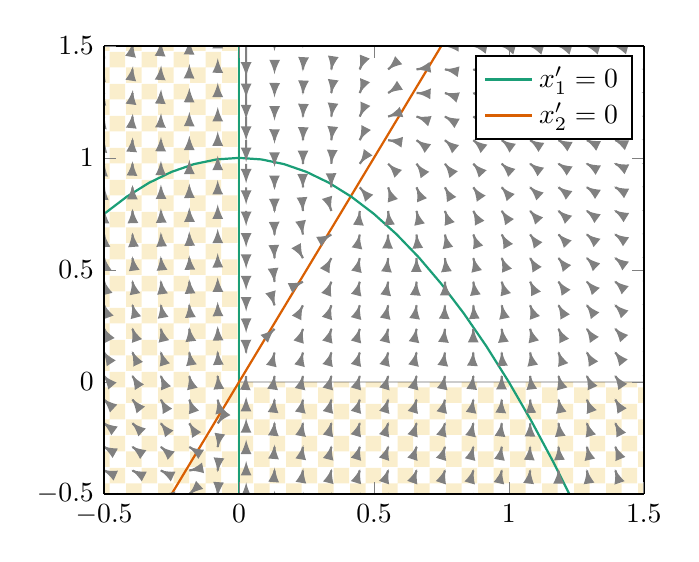
\begin{tikzpicture}
		\begin{axis}[
				view = {0}{90},
				xmin=-0.5, xmax=1.5, ymin=-0.5, ymax=1.5,
				domain=-0.5:1.5, y domain=-0.5:1.5,
				thick,
				]
				\draw[pattern=checkerboard, pattern color=Dark2-F, opacity=0.2] (0,0) -- (5,0) -- (5,-5) -- (-5,-5) -- (-5,5) -- (0,5) -- cycle;

				\def\r{1}
				\def\K{1}
				\def\J{0.5}

				\addplot[Dark2-A] coordinates {(0,-5)(0,5)};
				\addplot[Dark2-B, samples=2] {x / \J};
				\addplot[Dark2-A] {\r * (1 - x / \K) * (1 + x)};
				\legend{$x_1'=0$, $x_2'=0$}

				\addplot3 [gray, quiver={u={\r * x * (1 - x / \K) - x / (1 + x) * y}, v={1 - \J * y / x}, scale arrows=0.005, every arrow/.append style={-latex}}, samples=20] (x,y,0);
		\end{axis}
	\end{tikzpicture}
	\caption{Nullclines för systemet \eqref{eq:predator_prey_model} med riktningsfält för $r=1, K=1, J=1/2$. \label{fig:nullclines_2}}
\end{figure}

Med en nullcline på y\nobreakdash-axeln och det faktum att
flödet går uppåt längs x\nobreakdash-axeln då
$$ \left. \begin{pmatrix} 0 \\ 1 \end{pmatrix} \cdot x' \right\vert_{x = (x_1, 0)^T \ne 0} = 1 > 0 $$
kan vi, som för den första modellen, säga att
den öppna första kvadranten är positivt invariant.
Dessutom kan för varje val av $x(0)>0$ linjer $x_1=X_1$ och $x_2=X_2$
parallela med y- respektive x\nobreakdash-axeln väljas
sådana att
\begin{gather*}
	x_1(0) \le X_1, \quad K < X_1 \\
	x_2(0) \le X_2, \quad  \frac{X_1}J < X_2
\end{gather*}
för att få
$$ x_1' \overset{x_1 = X_1}< 0 \quad \text{och} \quad x_2' \overset{x_2 = X_2}< 0 $$
så att $R = \{x_1, x_2 > 0 \vert x_1 \le X_1, x_2 \le X_2\}$
är en positivt invariant mängd.
Det visar att varje lösning till \eqref{eq:predator_prey_model} med
$x(0)>0$ är begränsad, då $R$ är begränsad.

I fallet då jämviktspunkten $x^*$ i den öppna första kvadranten
är instabil existerar det en omgivning $U$ till $x^*$ sådan att
gränsvärdesmängden av en lösning som startar i $G \coloneqq R \setminus U$
inte innehåller $x^*$.
Då, enligt ovan, tillsammans med att jämviktspunkten i $x=0$ är instabil,
gör att alla positiva banor är begränsade med slutet hölje i $G$,
och då $G$ ej innehåller några jämviktspunkter
så finns det en periodisk lösning till \eqref{eq:predator_prey_model}
i $G$ enligt Poincaré-Bendixsons sats,
se figur~\ref{fig:phase_portrait2}.
Parametern $1/J$ bestämmer hur stor bytesdjurspopulationen behöver
vara för att försörja rovdjuren: Om $x_1/J < x_2$ kommer $x_2' < 0$.
Med ett för litet värde, som i figur~\ref{fig:phase_portrait2}.\subref{fig:mod2_unstable},
minskar rovdjurspopulationen snabbt när antalet bytesdjur blir litet,
och bytesdjuren tillåtes återhämta sig,
vilket speglas i att det blir cykler.

\begin{figure}
	\centering
	\renewcommand{\figurescale}{0.2}
	\subfloat[]{% This file was created by matlab2tikz.
%
%The latest updates can be retrieved from
%  http://www.mathworks.com/matlabcentral/fileexchange/22022-matlab2tikz-matlab2tikz
%where you can also make suggestions and rate matlab2tikz.
%
\definecolor{mycolor1}{rgb}{0.00000,0.44700,0.74100}%
\definecolor{mycolor2}{rgb}{0.85000,0.32500,0.09800}%
%
\begin{tikzpicture}

\begin{axis}[%
width=7.879in,
height=8.464in,
at={(1.322in,1.142in)},
scale only axis,
xmin=0,
xmax=8,
xlabel style={font=\color{white!15!black}},
xlabel={$\text{x}_\text{1}$},
ymin=0,
ymax=25,
ylabel style={font=\color{white!15!black}},
ylabel={$\text{x}_\text{2}$},
axis background/.style={fill=white},
axis x line*=bottom,
axis y line*=left,
legend style={legend cell align=left, align=left, draw=white!15!black},
scale=\figurescale
]
\addplot [color=mycolor1]
  table[row sep=crcr]{%
0	10\\
0.0808080808080808	10.6777255443018\\
0.161616161616162	11.3359587127113\\
0.242424242424242	11.9746995052287\\
0.323232323232323	12.5939479218538\\
0.404040404040404	13.1937039625868\\
0.484848484848485	13.7739676274276\\
0.565656565656566	14.3347389163762\\
0.646464646464647	14.8760178294326\\
0.727272727272727	15.3978043665968\\
0.808080808080808	15.9000985278688\\
0.888888888888889	16.3829003132486\\
0.96969696969697	16.8462097227362\\
1.05050505050505	17.2900267563316\\
1.13131313131313	17.7143514140348\\
1.21212121212121	18.1191836958458\\
1.29292929292929	18.5045236017647\\
1.37373737373737	18.8703711317913\\
1.45454545454545	19.2167262859257\\
1.53535353535354	19.543589064168\\
1.61616161616162	19.850959466518\\
1.6969696969697	20.1388374929759\\
1.77777777777778	20.4072231435416\\
1.85858585858586	20.656116418215\\
1.93939393939394	20.8855173169963\\
2.02020202020202	21.0954258398854\\
2.1010101010101	21.2858419868822\\
2.18181818181818	21.4567657579869\\
2.26262626262626	21.6081971531994\\
2.34343434343434	21.7401361725197\\
2.42424242424242	21.8525828159478\\
2.50505050505051	21.9455370834837\\
2.58585858585859	22.0189989751274\\
2.66666666666667	22.0729684908789\\
2.74747474747475	22.1074456307383\\
2.82828282828283	22.1224303947054\\
2.90909090909091	22.1179227827803\\
2.98989898989899	22.0939227949631\\
3.07070707070707	22.0504304312536\\
3.15151515151515	21.9874456916519\\
3.23232323232323	21.9049685761581\\
3.31313131313131	21.802999084772\\
3.39393939393939	21.6815372174938\\
3.47474747474747	21.5405829743234\\
3.55555555555556	21.3801363552607\\
3.63636363636364	21.2001973603059\\
3.71717171717172	21.0007659894589\\
3.7979797979798	20.7818422427197\\
3.87878787878788	20.5434261200883\\
3.95959595959596	20.2855176215647\\
4.04040404040404	20.0081167471489\\
4.12121212121212	19.7112234968409\\
4.2020202020202	19.3948378706407\\
4.28282828282828	19.0589598685483\\
4.36363636363636	18.7035894905637\\
4.44444444444444	18.3287267366869\\
4.52525252525253	17.934371606918\\
4.60606060606061	17.5205241012568\\
4.68686868686869	17.0871842197034\\
4.76767676767677	16.6343519622579\\
4.84848484848485	16.1620273289201\\
4.92929292929293	15.6702103196902\\
5.01010101010101	15.1589009345681\\
5.09090909090909	14.6280991735537\\
5.17171717171717	14.0778050366472\\
5.25252525252525	13.5080185238485\\
5.33333333333333	12.9187396351576\\
5.41414141414141	12.3099683705744\\
5.49494949494949	11.6817047300991\\
5.57575757575758	11.0339487137316\\
5.65656565656566	10.3667003214719\\
5.73737373737374	9.67995955332003\\
5.81818181818182	8.97372640927593\\
5.8989898989899	8.24800088933965\\
5.97979797979798	7.50278299351117\\
6.06060606060606	6.7380727217905\\
6.14141414141414	5.95387007417763\\
6.22222222222222	5.15017505067256\\
6.3030303030303	4.32698765127531\\
6.38383838383838	3.48430787598585\\
6.46464646464646	2.62213572480421\\
6.54545454545455	1.74047119773036\\
6.62626262626263	0.839314294764322\\
6.70707070707071	-0.0813349840939078\\
6.78787878787879	-1.02147663884435\\
6.86868686868687	-1.98111066948697\\
6.94949494949495	-2.96023707602178\\
7.03030303030303	-3.95885585844879\\
7.11111111111111	-4.976967016768\\
7.19191919191919	-6.01457055097942\\
7.27272727272727	-7.07166646108301\\
7.35353535353535	-8.14825474707882\\
7.43434343434343	-9.2443354089668\\
7.51515151515152	-10.359908446747\\
7.5959595959596	-11.4949738604194\\
7.67676767676768	-12.6495316499839\\
7.75757575757576	-13.8235818154407\\
7.83838383838384	-15.0171243567897\\
7.91919191919192	-16.2301592740308\\
8	-17.4626865671642\\
};

\addplot [color=mycolor2]
  table[row sep=crcr]{%
0	0\\
0.0808080808080808	0.023767082590612\\
0.161616161616162	0.047534165181224\\
0.242424242424242	0.071301247771836\\
0.323232323232323	0.095068330362448\\
0.404040404040404	0.11883541295306\\
0.484848484848485	0.142602495543672\\
0.565656565656566	0.166369578134284\\
0.646464646464647	0.190136660724896\\
0.727272727272727	0.213903743315508\\
0.808080808080808	0.23767082590612\\
0.888888888888889	0.261437908496732\\
0.96969696969697	0.285204991087344\\
1.05050505050505	0.308972073677956\\
1.13131313131313	0.332739156268568\\
1.21212121212121	0.35650623885918\\
1.29292929292929	0.380273321449792\\
1.37373737373737	0.404040404040404\\
1.45454545454545	0.427807486631016\\
1.53535353535354	0.451574569221628\\
1.61616161616162	0.47534165181224\\
1.6969696969697	0.499108734402852\\
1.77777777777778	0.522875816993464\\
1.85858585858586	0.546642899584076\\
1.93939393939394	0.570409982174688\\
2.02020202020202	0.5941770647653\\
2.1010101010101	0.617944147355912\\
2.18181818181818	0.641711229946524\\
2.26262626262626	0.665478312537136\\
2.34343434343434	0.689245395127748\\
2.42424242424242	0.71301247771836\\
2.50505050505051	0.736779560308972\\
2.58585858585859	0.760546642899584\\
2.66666666666667	0.784313725490196\\
2.74747474747475	0.808080808080808\\
2.82828282828283	0.83184789067142\\
2.90909090909091	0.855614973262032\\
2.98989898989899	0.879382055852644\\
3.07070707070707	0.903149138443256\\
3.15151515151515	0.926916221033868\\
3.23232323232323	0.95068330362448\\
3.31313131313131	0.974450386215092\\
3.39393939393939	0.998217468805704\\
3.47474747474747	1.02198455139632\\
3.55555555555556	1.04575163398693\\
3.63636363636364	1.06951871657754\\
3.71717171717172	1.09328579916815\\
3.7979797979798	1.11705288175876\\
3.87878787878788	1.14081996434938\\
3.95959595959596	1.16458704693999\\
4.04040404040404	1.1883541295306\\
4.12121212121212	1.21212121212121\\
4.2020202020202	1.23588829471182\\
4.28282828282828	1.25965537730244\\
4.36363636363636	1.28342245989305\\
4.44444444444444	1.30718954248366\\
4.52525252525253	1.33095662507427\\
4.60606060606061	1.35472370766488\\
4.68686868686869	1.3784907902555\\
4.76767676767677	1.40225787284611\\
4.84848484848485	1.42602495543672\\
4.92929292929293	1.44979203802733\\
5.01010101010101	1.47355912061794\\
5.09090909090909	1.49732620320856\\
5.17171717171717	1.52109328579917\\
5.25252525252525	1.54486036838978\\
5.33333333333333	1.56862745098039\\
5.41414141414141	1.592394533571\\
5.49494949494949	1.61616161616162\\
5.57575757575758	1.63992869875223\\
5.65656565656566	1.66369578134284\\
5.73737373737374	1.68746286393345\\
5.81818181818182	1.71122994652406\\
5.8989898989899	1.73499702911468\\
5.97979797979798	1.75876411170529\\
6.06060606060606	1.7825311942959\\
6.14141414141414	1.80629827688651\\
6.22222222222222	1.83006535947712\\
6.3030303030303	1.85383244206774\\
6.38383838383838	1.87759952465835\\
6.46464646464646	1.90136660724896\\
6.54545454545455	1.92513368983957\\
6.62626262626263	1.94890077243018\\
6.70707070707071	1.9726678550208\\
6.78787878787879	1.99643493761141\\
6.86868686868687	2.02020202020202\\
6.94949494949495	2.04396910279263\\
7.03030303030303	2.06773618538324\\
7.11111111111111	2.09150326797386\\
7.19191919191919	2.11527035056447\\
7.27272727272727	2.13903743315508\\
7.35353535353535	2.16280451574569\\
7.43434343434343	2.1865715983363\\
7.51515151515152	2.21033868092692\\
7.5959595959596	2.23410576351753\\
7.67676767676768	2.25787284610814\\
7.75757575757576	2.28163992869875\\
7.83838383838384	2.30540701128936\\
7.91919191919192	2.32917409387998\\
8	2.35294117647059\\
};

\addplot [color=red, draw=none, mark=o, mark options={solid, red}]
  table[row sep=crcr]{%
6.52911408622764	1.9203276724199\\
};

\addplot [color=blue]
  table[row sep=crcr]{%
0.555555555555555	22.8910098522167\\
0.531869956247764	21.74483213281\\
0.511613914720607	20.6115905576569\\
0.494587766679078	19.4989121343292\\
0.480598729215109	18.4139794118008\\
0.455508655054245	15.4519710193685\\
0.450969808047591	12.8965922736018\\
0.464144883563707	10.7960660179284\\
0.493734735517913	9.11889615665879\\
0.535040175575874	7.89382539731086\\
0.590221739560162	6.92206412569504\\
0.660155256786466	6.15423336593679\\
0.746080476104425	5.54775942729808\\
0.943697057485638	4.75861390906284\\
1.20783392626972	4.23225222001215\\
1.5464416629647	3.87491476748733\\
1.96201566840309	3.62496185544838\\
2.65304591766989	3.39324443305319\\
3.41680812841654	3.24424516506205\\
4.17012372433563	3.14340728355078\\
4.83469640808431	3.06997161933043\\
5.19656713424737	3.03144242389347\\
5.49408826585992	2.99837617899479\\
5.73026608906681	2.96934201714956\\
5.91295348152757	2.9432113236498\\
6.0533478423496	2.91917884488752\\
6.15886546646491	2.89683756827567\\
6.23610620362103	2.87586048966623\\
6.29271481651895	2.85589068417249\\
6.33629801391627	2.83624780797181\\
6.36807589170938	2.81732389735887\\
6.39060859990777	2.7990300408573\\
6.40704802654407	2.78125839907963\\
6.42227252693577	2.76044371988865\\
6.43295174696994	2.74024383170904\\
6.43996904037667	2.72062130625558\\
6.44511212928359	2.70151519526481\\
6.45090837314395	2.67810548499429\\
6.4551600937942	2.65543779746941\\
6.45792767466246	2.63348799724578\\
6.46028337113349	2.61220839243633\\
6.46402012026578	2.58482968274828\\
6.46707834758381	2.55855690982215\\
6.46917773614757	2.53335178538365\\
6.47125650757592	2.50915008823375\\
6.47563206769336	2.4777316215769\\
6.47895925723813	2.4480198437453\\
6.48019819686607	2.41994507591487\\
6.48190738937259	2.39336481709599\\
6.49133624676732	2.36450247904623\\
6.4957592863988	2.33749562657445\\
6.48873856252948	2.31236386538671\\
6.48603735838352	2.28868436880046\\
6.49197300529649	2.27544061659489\\
6.49551368954836	2.26271797962022\\
6.4959614105879	2.25051253029405\\
6.49635964558078	2.23874526010932\\
6.49865795666609	2.22736092595888\\
6.50031235463926	2.21639602342276\\
6.5011488683608	2.20583912113055\\
6.50194922058814	2.19566049411103\\
6.50422311421623	2.18192462515609\\
6.50581006727975	2.16888688923802\\
6.50603444994915	2.15652564020484\\
6.5065725196197	2.14477585804894\\
6.51276886122795	2.13092561738114\\
6.51530535303435	2.11798827054273\\
6.5093851986833	2.10599914005372\\
6.50679394525653	2.09469074994655\\
6.51124522495498	2.08816772743618\\
6.51366226553372	2.08192216505875\\
6.51324415478258	2.07595947763658\\
6.51293733147588	2.07021598273097\\
6.51465225146316	2.06464811508242\\
6.5157265862093	2.05929744983242\\
6.5159187570871	2.05416066870909\\
6.51613471338562	2.04921375545536\\
6.5178415991779	2.04271588647422\\
6.51879810669943	2.03655728634082\\
6.51819905090555	2.03073591127833\\
6.51802469114809	2.0252004156171\\
6.52384535372391	2.01881572671487\\
6.52582120222765	2.01287663477278\\
6.51887243639844	2.00744852197931\\
6.51542218849927	2.00229119564957\\
6.51972355503063	1.99921390400053\\
6.52191423355597	1.99628494461664\\
6.52117878012931	1.99351436012518\\
6.52055721650823	1.99084379265002\\
6.52201652108145	1.98823458640345\\
6.52283192818019	1.98573176506571\\
6.52276319558118	1.98333601523911\\
6.52272441816472	1.98102779106478\\
6.52407886144565	1.97798750450589\\
6.52471431265223	1.97511015361599\\
6.52384957206996	1.97240181845037\\
6.5234069886984	1.96982174648284\\
6.52869282730238	1.96677936737955\\
6.53031179364702	1.96397678683915\\
6.52339921749378	1.96148598401677\\
6.51984312375576	1.95909252212375\\
6.52389511029509	1.95759584628559\\
6.52587792392175	1.95618828209291\\
6.52495102409238	1.95488219703735\\
6.52416739476021	1.9536222215748\\
6.52550852930765	1.95237212096883\\
6.52619914925039	1.95117869312489\\
6.52598251920117	1.95004467018269\\
6.52580896388899	1.94895192494568\\
6.52703925690972	1.94750992557648\\
6.5275379773848	1.94615125682518\\
6.52650063987949	1.94488618952396\\
6.52590526259153	1.94367729403785\\
6.53102672678969	1.94220750734863\\
6.53250853022894	1.94088194009115\\
6.52552070017478	1.93977675180323\\
6.52185190329857	1.93868688988365\\
6.52582995628427	1.93794356984933\\
6.52773715848027	1.9372612492216\\
6.52671744801471	1.93665347390614\\
6.52585288907301	1.93606590479718\\
6.5271461615782	1.93546322695408\\
6.52778193935406	1.93489337839614\\
6.52749552777595	1.93436007957646\\
6.52725777328038	1.93384584278501\\
6.52842680926668	1.93315653477334\\
6.52886098539465	1.93251305094766\\
6.52774997859859	1.93192753966336\\
6.5270864213843	1.93136433865843\\
6.53208389997364	1.93062939098181\\
6.53348990257305	1.92999386293102\\
6.52653963496932	1.92953501429607\\
6.5228549420851	1.92905413720167\\
6.5267760647893	1.9286671863339\\
6.52863383829827	1.92832779536068\\
6.52755915555883	1.92805016175591\\
6.52665078542659	1.92778039392151\\
6.52792512796604	1.92748355492001\\
6.52853566036481	1.92720832131658\\
6.52820969826177	1.92695895195521\\
6.52793725618513	1.92671810166941\\
6.5290854202289	1.92638269560135\\
6.52949191929147	1.92607562218263\\
6.52833782868299	1.92581000450552\\
6.52763702136165	1.92555076267719\\
6.53257365325676	1.92516136755815\\
6.53394548540393	1.92485035411571\\
6.5270267107037	1.92469534964868\\
6.52333774863643	1.92450099897189\\
6.52723161677775	1.92428307004162\\
6.52906470502852	1.92410632430516\\
6.5279580820507	1.92398532970521\\
6.52702528384674	1.92386629297909\\
6.52829437255984	1.92371437157887\\
6.52889430211123	1.92357875750865\\
6.52854653292883	1.92346400073931\\
6.52825550711132	1.92335273432106\\
6.52939691535546	1.92318418853703\\
6.52979157529722	1.92303576779645\\
6.52861493435862	1.92292107980159\\
6.52789497209226	1.92280524964785\\
6.53279086997208	1.92257862422941\\
6.53414458306959	1.92242035316066\\
6.52726384001507	1.92240798275254\\
6.52358285655566	1.92234837247264\\
6.52745861481747	1.92221060603669\\
6.52927625365576	1.92211097011539\\
6.52814912474745	1.92206425955483\\
6.52720172707209	1.92201666319455\\
6.52847100780246	1.921933328272\\
6.52906673484376	1.92186381796655\\
6.52870558445168	1.92181285440938\\
6.52840368048267	1.92176297824318\\
6.52954527390673	1.92167311646193\\
6.52993556846738	1.92159954752773\\
6.52874521190119	1.92155614328153\\
6.52801421554218	1.92150803415924\\
6.5328844437151	1.92135821944553\\
6.53422896483538	1.92127194944296\\
6.52738064078554	1.92132657673889\\
6.5237090366705	1.92133040447128\\
6.52757361181652	1.92123065945824\\
6.52938180423751	1.92116758740876\\
6.52824096205106	1.92115612995289\\
6.52728431667453	1.9211424089362\\
6.52855588133857	1.92109151953927\\
6.52915034019437	1.92105330176037\\
6.52878062422404	1.92103258440093\\
6.52847203868841	1.92101180235253\\
6.52961610074255	1.92095905571121\\
6.53000521879836	1.92092081906873\\
6.52880635415893	1.92091111265258\\
6.52806879604473	1.92089500836504\\
6.53292095832285	1.92078151569365\\
6.53426035269287	1.9207292181113\\
6.52743976915825	1.92081524315788\\
6.5237776535871	1.92084891902003\\
6.52763445253527	1.92076722204461\\
6.52943625808783	1.9207214965905\\
6.52828570756814	1.92072678501347\\
6.52732283508446	1.9207291334309\\
6.52859719750637	1.92069357604649\\
6.52919160628091	1.92067016349258\\
6.5288160125502	1.92066379551251\\
6.52850301756169	1.92065680673194\\
6.5296502145695	1.92062155878802\\
6.53003950139618	1.92060000033977\\
6.52883489450984	1.92060624184465\\
6.52809310169288	1.92060527603126\\
6.5329322994578	1.92050899721801\\
6.53426873223172	1.92047274152562\\
6.527470743577	1.92057342858331\\
6.52381691407964	1.92062113330933\\
6.5276681996575	1.9205480124678\\
6.52946554061923	1.92051052359064\\
6.52830787161222	1.92052378130588\\
6.52734059449038	1.92053376036583\\
6.52861765026465	1.92050543696133\\
6.52921247876215	1.92048902455172\\
6.52883267191967	1.92048947250946\\
6.52851661027896	1.92048902837275\\
6.5296668255374	1.92046202231348\\
6.53005675997696	1.92044833474531\\
6.5288481084468	1.92046213434627\\
6.52810343435806	1.92046833655129\\
6.53293292881757	1.92038024375306\\
6.53426751087087	1.92035156931676\\
6.5274877918444	1.9204590533577\\
6.52384094193868	1.92051333376424\\
6.52768813171055	1.92044429773458\\
6.52948219902353	1.92041072690976\\
6.52831915792161	1.92042778962166\\
6.52734864207257	1.92044139887606\\
6.52862805899898	1.92041648035287\\
6.52922343683376	1.92040337463893\\
6.52884049366068	1.92040706739712\\
6.52852219927361	1.92040973334533\\
6.52967506914682	1.92038660127478\\
6.53006576293163	1.92037662563667\\
6.52885413289402	1.92039401512326\\
6.52810739240469	1.92040361669525\\
6.53292948870935	1.92031943634816\\
6.5342628452285	1.92029434799568\\
6.52749775063683	1.92040494283281\\
6.52385661279813	1.92046229061225\\
6.52770069665611	1.920395207688\\
6.52949230055887	1.92036350640696\\
6.52832512962861	1.9203823959811\\
6.52735216608652	1.92039773792739\\
6.52863356545233	1.92037441566612\\
6.5292294829031	1.92036286973701\\
6.528844147798	1.92036811314939\\
6.52852417593311	1.92037226102536\\
6.5296792752771	1.92035094330219\\
6.53007068796992	1.9203427159202\\
6.52885680483124	1.92036181639022\\
6.52810852900356	1.92037303399233\\
6.53292489023372	1.9202907387432\\
6.5342573868551	1.92026734881636\\
6.5275039667355	1.92037933407386\\
6.5238674499923	1.92043810020802\\
6.52770913395518	1.9203719573648\\
6.52949884457316	1.92034115293635\\
6.52832845773381	1.92036092777056\\
6.52735360914448	1.92037710133344\\
6.52863663538277	1.92035452244976\\
6.52923303076467	1.92034371061057\\
6.52884584042637	1.92034969987187\\
6.52852458011249	1.92035455712562\\
6.52968150996847	1.92033408372795\\
6.53007354931547	1.92032667779238\\
6.52885792760391	1.92034659834624\\
6.52810848091703	1.92035858723231\\
6.53292035422684	1.92027721190722\\
6.53425222186539	1.92025462787066\\
6.52750810305295	1.92036720716355\\
6.52387529701175	1.92042661898208\\
6.52771510681062	1.92036093355105\\
6.5295033436075	1.92033056316488\\
6.5283304316867	1.92035077341893\\
6.52735411320125	1.92036734980232\\
6.52863845819695	1.92034511314217\\
6.52923525717405	1.92033464549244\\
6.52884661258017	1.92034099732768\\
6.52852434847811	1.92034619675565\\
6.52968276227116	1.92032611188893\\
6.5300753263602	1.92031909032521\\
6.52885834657503	1.92033940754815\\
6.52810799198047	1.92035176691521\\
6.53291632945141	1.92027084955684\\
6.53424772251498	1.92024864903189\\
6.52751101123202	1.92036145893073\\
6.52388117459707	1.92042115634127\\
6.52771950957639	1.92035569736617\\
6.52950658891346	1.92032554005923\\
6.52833168337253	1.92034596951154\\
6.52735420936165	1.92036274392397\\
6.52863961604901	1.92034066161091\\
6.52923674748128	1.92033035431221\\
6.52884695512782	1.9203368854228\\
6.52852390180573	1.920342251969\\
6.52968351034397	1.92032234232112\\
6.53007650470726	1.92031549931599\\
6.52885845546616	1.92033601122702\\
6.52810738912808	1.9203485504148\\
6.53291292899813	1.92026786799532\\
6.53424395660036	1.92024585084243\\
6.52751314455853	1.92035872981035\\
6.52388567965226	1.9204185466181\\
6.52772284854172	1.92035320278207\\
6.52950901380084	1.92032315243958\\
6.52833252853332	1.92034369611048\\
6.52735414132823	1.92036057014863\\
6.52864039952255	1.92033855482886\\
6.52923780113493	1.92032832141211\\
6.52884709903424	1.92033494351657\\
6.52852342161369	1.92034039330652\\
6.52968398836081	1.92032055974657\\
6.53007733147632	1.92031379863959\\
6.52885843581068	1.92033440830056\\
6.52810680768317	1.92034703622646\\
6.53291012759975	1.92026647958593\\
6.53424086995461	1.92024455078662\\
6.52751475742382	1.92035743058145\\
6.52388918536659	1.92041729139689\\
6.52772542929156	1.92035200841292\\
6.52951087000499	1.92032201358404\\
6.5283331299299	1.92034261967683\\
6.52735401854994	1.9203595455835\\
6.52864095825949	1.92033755715071\\
6.5292385777854	1.92032735711053\\
6.52884715262043	1.92033402719822\\
6.52852297987722	1.92033951970994\\
6.52968431352543	1.92031971673517\\
6.53007793749494	1.9203129923364\\
6.52885836975442	1.92033365276315\\
6.52810629627342	1.92034632561227\\
6.5329078511895	1.92026584016938\\
6.534238369008	1.92024395447097\\
6.52751600169787	1.92035680928308\\
6.52389193986407	1.92041668098685\\
6.52772744853366	1.92035143188094\\
6.52951231354665	1.92032146723165\\
6.52833357510889	1.92034210954579\\
6.52735388814133	1.92035906377007\\
6.52864137270879	1.92033708422233\\
6.52923916724406	1.92032689871607\\
6.52884716638777	1.9203335954454\\
6.52852259962237	1.92033911083641\\
6.52968454637514	1.92031931802078\\
6.53007839569645	1.92031260937053\\
6.52885829321854	1.92033329743004\\
6.52810586572555	1.92034599388723\\
6.53290601546406	1.92026555146585\\
6.53423635558459	1.92024368720672\\
6.52751697421265	1.92035650996716\\
6.52389411732065	1.9204163789069\\
6.52772904068583	1.92035114988974\\
6.52951344752228	1.92032120264382\\
6.52833391384885	1.92034186743299\\
6.52735376869539	1.92035883807026\\
6.52864168862236	1.92033685966547\\
6.52923962337193	1.92032668003335\\
6.52884716364123	1.92033339251455\\
6.52852228297615	1.92033892086086\\
6.52968471960623	1.920319129414\\
6.53007874937687	1.92031242692626\\
6.52885822086442	1.92033313094853\\
6.52810551147858	1.92034584045802\\
6.53290454145143	1.92026542584648\\
6.53423474046804	1.92024357257129\\
6.52751774059541	1.92035636402647\\
6.52389584519541	1.92041622534508\\
6.52773030215925	1.92035100907347\\
6.52951434394881	1.92032107255602\\
6.52833417632731	1.92034175223983\\
6.52735366606334	1.92035873304977\\
6.52864193376812	1.92033675274251\\
6.529239980704	1.9203265750902\\
6.52884715493913	1.92033329753795\\
6.5285220239667	1.92033883371589\\
6.52968485191485	1.92031904017351\\
6.53007902601655	1.92031233957435\\
6.52885815777597	1.92033305345748\\
6.52810522367412	1.92034577064728\\
6.5329033607172	1.92026537514648\\
6.53423344744925	1.9202435277411\\
6.52751834763938	1.92035629150269\\
6.52389721960663	1.9204161441773\\
6.52773130465398	1.9203509365236\\
6.52951505537284	1.92032100707377\\
6.52833438208516	1.92034169720685\\
6.52735358066764	1.9203586847519\\
6.528642126162	1.92033670159377\\
6.52924026279287	1.92032652424017\\
6.52884714490411	1.92033325341161\\
6.52852181420865	1.92033879465475\\
6.52968495471743	1.92031899793107\\
6.53007924419135	1.92031229740604\\
6.52885810488449	1.92033301779892\\
6.52810499151549	1.92034573982509\\
6.53290241616162	1.92026535812007\\
6.53423241342104	1.92024351403013\\
6.52751883000519	1.92035625440464\\
6.52389831452425	1.92041609896745\\
6.5277321028478	1.92035089745741\\
6.52951562135436	1.92032097294195\\
6.52833454455209	1.92034167073573\\
6.52735351083731	1.92035866300232\\
6.52864227821638	1.92033667693745\\
6.52924048653219	1.92032649921585\\
6.52884713542552	1.92033323317278\\
6.52852164530183	1.9203387778988\\
6.52968503546396	1.92031897792128\\
6.53007941713293	1.92031227677722\\
6.52885806145665	1.92033300172344\\
6.52810480500783	1.9203457269987\\
6.53290166108085	1.92026535561753\\
6.53423158698238	1.92024351352649\\
6.52751921406026	1.92035623462361\\
6.52389918763673	1.92041607213681\\
6.52773273913835	1.92035087518371\\
6.52951607231584	1.92032095427306\\
6.52833467341215	1.92034165786115\\
6.5273534542893	1.92035865358758\\
6.52864239890513	1.9203366649031\\
6.52924066450107	1.92032648660064\\
6.5288471271593	1.92033322410341\\
6.52852150973587	1.92033877134522\\
6.5296850993126	1.92031896843156\\
6.53007955464474	1.92031226647231\\
6.52885802620973	1.92033299474993\\
6.52810465552577	1.92034572233012\\
6.53290105768763	1.9202653588659\\
6.53423092664557	1.92024351806444\\
6.52751952022166	1.92035622348214\\
6.52389988432033	1.92041605509496\\
6.52773324675625	1.92035086161591\\
6.52951643197921	1.92032094342536\\
6.52833477589946	1.92034165148804\\
6.52735340875222	1.92035864983061\\
6.52864249494822	1.92033665891271\\
6.52924080631018	1.92032648001055\\
6.52884712022551	1.92033322021495\\
6.52852140113561	1.92033876934049\\
6.52968515000654	1.920318963922\\
6.53007966419171	1.92031226115987\\
6.52885799779048	1.92033299195407\\
6.52810453588006	1.92034572123815\\
6.53290057559263	1.92026536394192\\
6.5342303990919	1.92024352402533\\
6.52751976448034	1.9203562167859\\
6.52390044046138	1.92041604355825\\
6.52773365192566	1.92035085277569\\
6.52951671900565	1.92032093668252\\
6.52833485755052	1.9203416482467\\
6.52735337220039	1.92035864860925\\
6.52864257149958	1.92033665584054\\
6.52924091942699	1.92032647639512\\
6.5288471145288	1.92033321869587\\
6.52852131423241	1.92033876926668\\
6.52968519035624	1.92031896177181\\
6.53007975156147	1.92031225829658\\
6.52885797496314	1.92033299103275\\
6.52810444018871	1.92034572161305\\
6.53290019043734	1.92026536917006\\
6.53422997763681	1.92024352989165\\
6.52751995945144	1.92035621247892\\
6.52390088453932	1.92041603532443\\
6.52773397543109	1.92035084665871\\
6.52951694815728	1.92032093220529\\
6.52833492267034	1.92034164653212\\
6.527353342916	1.92035864847525\\
6.52864263257385	1.92033665419641\\
6.52924100971586	1.92032647428663\\
6.52884710990238	1.9203332182329\\
6.5285212447351	1.92033876993017\\
6.529685222521	1.92031896074084\\
6.53007982129297	1.92031225666197\\
6.52885795666769	1.92033299091724\\
6.52810436368874	1.92034572250236\\
6.53289988273264	1.92026537390143\\
6.53422964094044	1.92024353510034\\
6.52752011513227	1.92035620953115\\
6.52390123920575	1.92041602921122\\
6.52773423379104	1.92035084221894\\
6.52951713115285	1.92032092905855\\
6.52833497464038	1.92034164557607\\
6.5273533194798	1.92035864876623\\
6.52864268132895	1.920336653266\\
6.52924108181286	1.92032647297086\\
6.52884710617003	1.92033321821797\\
6.52852118917732	1.92033877080189\\
6.5296852481847	1.92031896024194\\
6.53007987697138	1.92031225566477\\
6.5288579420231	1.92033299111838\\
6.52810430254572	1.92034572349176\\
6.53289963690012	1.92026537794366\\
6.53422937194995	1.92024353950853\\
6.52752023946828	1.92035620740929\\
6.5239015225031	1.92041602454706\\
6.52773444015669	1.92035083888336\\
6.52951727731583	1.92032092674797\\
6.52833501613353	1.92034164500791\\
6.52735330073584	1.92035864918693\\
6.52864272026394	1.92033665270379\\
6.52924113939799	1.92032647209398\\
6.52884710317058	1.92033321837388\\
6.52852114477201	1.92033877165991\\
6.52968526867286	1.9203189599969\\
6.53007992144102	1.92031225501401\\
6.52885793030948	1.92033299141782\\
6.52810425368297	1.92034572441413\\
6.53289944049339	1.92026538129717\\
6.53422915704329	1.92024354314716\\
6.52752033878557	1.92035620582433\\
6.52390174881603	1.9204160209246\\
6.52773460501025	1.9203508363184\\
6.52951739407452	1.92032092499813\\
6.52833504927093	1.92034164464651\\
6.52735328575022	1.92035864961206\\
6.52864275136382	1.92033665234025\\
6.52924118539963	1.9203264714758\\
6.5288471007656	1.92033321857781\\
6.52852110928436	1.92033877242185\\
6.52968528503489	1.92031895987373\\
6.53007995696452	1.92031225456309\\
6.52885792094421	1.92033299172268\\
6.52810421463656	1.92034572521345\\
6.53289928357031	1.92026538403514\\
6.53422898534029	1.92024354610949\\
6.52752041812686	1.92035620461014\\
6.52390192962055	1.92041601807953\\
6.52773473671297	1.92035083431636\\
6.52951748735271	1.92032092364554\\
6.52833507573999	1.92034164440151\\
6.5273532737719	1.92035864999381\\
6.52864277620887	1.92033665209027\\
6.52924122215169	1.92032647102084\\
6.52884709883985	1.92033321877827\\
6.52852108092512	1.92033877306676\\
6.52968529810458	1.92031895980965\\
6.5300799853448	1.92031225423543\\
6.52885791345829	1.92033299199727\\
6.52810418343531	1.92034572588158\\
6.53289915818983	1.92026538625048\\
6.53422884815125	1.92024354850247\\
6.52752048151479	1.92035620366468\\
6.52390207407585	1.92041601582958\\
6.52773484193748	1.92035083273909\\
6.52951756187723	1.92032092258634\\
6.52833509688517	1.92034164422645\\
6.52735326419854	1.92035865031874\\
6.5286427960589	1.92033665190966\\
6.52924125151599	1.92032647067573\\
6.52884709729907	1.92033321895618\\
6.52852105826306	1.92033877359914\\
6.52968530854583	1.92031895977467\\
6.53008000801991	1.92031225398903\\
6.52885790747541	1.92033299223133\\
6.52810415850323	1.92034572642938\\
6.53289905800899	1.92026538803367\\
6.53422873853544	1.92024355042682\\
6.52752053215995	1.9203562029209\\
6.52390218949463	1.92041601404283\\
6.52773492601091	1.9203508314894\\
6.52951762142138	1.92032092175018\\
6.52833511377868	1.92034164409636\\
6.52735325654782	1.92035865058777\\
6.5286428119191	1.92033665177439\\
6.52924127497867	1.92032647040868\\
6.52884709606688	1.92033321910672\\
6.52852104015389	1.92033877403261\\
6.529685316888	1.92031895975439\\
6.53008002613764	1.92031225379944\\
6.52885790269414	1.92033299242529\\
6.52810413858067	1.92034572687368\\
6.53289897796115	1.92026538946469\\
6.53422865094885	1.92024355197028\\
6.52752057262567	1.92035620233211\\
6.52390228171653	1.92041601262035\\
6.52773499318714	1.92035083049586\\
6.52951766899814	1.92032092108688\\
6.52833512727622	1.92034164399703\\
6.52735325043383	1.92035865080719\\
6.52864282459194	1.92033665167058\\
6.52924129372643	1.9203264701994\\
6.52884709508177	1.92033321923097\\
6.52852102568296	1.92033877438279\\
6.52968532355345	1.9203189597418\\
6.53008004061445	1.92031225365139\\
6.52885789887329	1.92033299258355\\
6.52810412266103	1.92034572723182\\
6.52892031513107	1.92033179486358\\
6.52928452884463	1.92032558067103\\
6.52895772572596	1.92033114322074\\
6.52870423930514	1.92033544287486\\
};

\addplot [color=blue]
  table[row sep=crcr]{%
1.67724867724868	24.4919950738916\\
1.61551246254366	23.2689662311692\\
1.57033272764989	22.0696495531895\\
1.54160328347333	20.9066457208133\\
1.5292616398241	19.791505430878\\
1.5706275464726	17.2526749082488\\
1.72034076273726	15.1629629943245\\
1.9815973290385	13.5277631477312\\
2.35261748825842	12.2914776824825\\
2.82376390514657	11.3569905022681\\
3.35486713403917	10.6443282336658\\
3.89641511554238	10.0857867232183\\
4.39806276003035	9.63238007670534\\
4.69342601943077	9.36755850489728\\
4.94711993423937	9.12810722985589\\
5.15855023360257	8.90847396266287\\
5.3308143954381	8.7043631784709\\
5.47005937524459	8.51260059381958\\
5.58102924615057	8.33118259043138\\
5.66828760021696	8.15856309432055\\
5.73746686433105	7.99326387154671\\
5.79848328476631	7.82045842026171\\
5.84703581020901	7.65440717451833\\
5.88548054367326	7.49452597386278\\
5.91728146312936	7.34015527406746\\
5.94863897424275	7.17220521065049\\
5.97528148040873	7.0103362431348\\
5.99790939421714	6.85422396962077\\
6.01822393218896	6.70348393002679\\
6.04227245123966	6.52257948572581\\
6.06396123648036	6.34920778837668\\
6.08326291992575	6.18300716402986\\
6.10140511085193	6.0235548531679\\
6.12450385324994	5.82824774641621\\
6.14565355155739	5.6429241628624\\
6.16442435685884	5.46703581801154\\
6.18225809144147	5.2999676971102\\
6.20569460577675	5.10279124080398\\
6.22631146628144	4.91779468481053\\
6.24250501722919	4.74423448195786\\
6.25841174797316	4.58116059454671\\
6.28114259155446	4.42247367954477\\
6.29860360043932	4.27377774037321\\
6.30566304345576	4.13461153682498\\
6.31492880458189	4.00387109540057\\
6.33384814501241	3.90071184125801\\
6.34704298010077	3.80298548491256\\
6.34962840783046	3.7105654289793\\
6.35404158486035	3.62274822937825\\
6.36556446868802	3.55390525812984\\
6.37437228269237	3.48799054550736\\
6.37936991729888	3.42491150816035\\
6.38433442095534	3.36442610672388\\
6.39201615847489	3.30496248933605\\
6.39851398639217	3.2480253753923\\
6.4033520068322	3.19351857357395\\
6.40809416496124	3.14129097846091\\
6.41563684566982	3.08013724392158\\
6.42194561589322	3.02212263134111\\
6.42608999304249	2.96710805929122\\
6.43044291753127	2.91487407560886\\
6.44001828324721	2.85794375223118\\
6.4465082349192	2.80437658422796\\
6.44644908484917	2.75406064194847\\
6.44828997688652	2.70660251537366\\
6.4548951487129	2.67433653831813\\
6.45944649915108	2.64345067965392\\
6.46081773249245	2.61391373121326\\
6.46243984105047	2.58558970513977\\
6.46666706671705	2.55837234447477\\
6.46990934085705	2.53229682223151\\
6.47165674628137	2.50732713823639\\
6.47347615282963	2.48338252897107\\
6.47776500597105	2.45524048989328\\
6.4809101763835	2.42853492966599\\
6.48183491730792	2.40321649788602\\
6.48322223290014	2.37915886687031\\
6.49014871826435	2.3534012830055\\
6.49383407654738	2.32915291000695\\
6.49036299705655	2.30640984190172\\
6.48923714735287	2.28490034473618\\
6.49430724464773	2.27042331936466\\
6.4972958900245	2.25656025134448\\
6.49710532386794	2.24330934706702\\
6.49719280629043	2.2305785978675\\
6.49988451119381	2.21830063271683\\
6.50169810214236	2.206525055073\\
6.50218935128115	2.19524093956031\\
6.50277404774628	2.18440173793736\\
6.50542884223889	2.17137759483762\\
6.50710990318836	2.15901316973291\\
6.50684136414269	2.14729499583491\\
6.50704677018204	2.13614640134875\\
6.51258412715939	2.12391330077971\\
6.51497185545011	2.11242413279841\\
6.51026006395761	2.10171189275722\\
6.50802732017355	2.09156245970262\\
6.51231661938231	2.08481355688225\\
6.51457505067162	2.07836383735624\\
6.51373718615679	2.07222213201392\\
6.51318762038549	2.0663156781294\\
6.5151927897584	2.06059340226716\\
6.51637426238653	2.0551086676494\\
6.51631277240426	2.04986026165407\\
6.5163569542085	2.04481509209735\\
6.51830362463766	2.03867504647441\\
6.519331776189	2.03285209439569\\
6.51848102118381	2.0273485232292\\
6.51812786377362	2.02210745346747\\
6.52313529828528	2.01628179134744\\
6.52495048841168	2.01083723123037\\
6.51949878281498	2.00582613493401\\
6.51665869411283	2.00105697394328\\
6.5206461444361	1.99787483061416\\
6.52260279279412	1.99484953267961\\
6.52148835767567	1.99199441742472\\
6.52065468986909	1.98924526830881\\
6.52233417194673	1.98655837563933\\
6.52322319334976	1.98398829010862\\
6.52292688624023	1.98153790048519\\
6.52273461190816	1.9791806023392\\
6.52432684987358	1.97626985292668\\
6.52504233448491	1.97351608493615\\
6.52394598297929	1.97092855043211\\
6.52334807650013	1.96846026448938\\
6.52810848658076	1.96565255411626\\
6.52965015914886	1.96305530776996\\
6.5238218817066	1.96073019555417\\
6.52069048970005	1.95849561257231\\
6.52453793559554	1.95696850757838\\
6.52635753033998	1.95553311799622\\
6.52513017228995	1.9542046353229\\
6.5241742279074	1.95292303694704\\
6.52569208466484	1.95164818970573\\
6.5264415524803	1.95043469057161\\
6.52604513124033	1.94928717204783\\
6.52574918573449	1.94818222729426\\
6.52716687131501	1.94679299523319\\
6.52773218657702	1.94548552465421\\
6.52652565767835	1.94427225775215\\
6.52581655179219	1.94311098147907\\
6.53048864593274	1.94173649705581\\
6.5319058328034	1.940491459242\\
6.52584459386244	1.93944257282039\\
6.52255087002786	1.93841149624095\\
6.52634547272988	1.93765940979101\\
6.52811006203445	1.93696884079217\\
6.52684332450869	1.93635569979688\\
6.52583754434263	1.93576207599745\\
6.52727154693171	1.93514964719301\\
6.52795310600181	1.93457266704326\\
6.5275190426188	1.93403646660682\\
6.52718073273248	1.93351936906969\\
6.52850598026831	1.93285016626006\\
6.52899668941879	1.93222704633389\\
6.52774692268882	1.93166385622604\\
6.52699104599478	1.93112089437419\\
6.53163822720991	1.93042710692146\\
6.53299811734342	1.92982436720932\\
6.52678790433328	1.9293821950834\\
6.52340171037093	1.92892277088484\\
6.52717866039405	1.92853463238313\\
6.52892324661781	1.92819393497979\\
6.52764918052172	1.92791680999738\\
6.52662638748576	1.92764649881399\\
6.52801403850609	1.92734566538753\\
6.52866139171429	1.92706809589673\\
6.52821679362107	1.92681936402856\\
6.52786343073988	1.92657879871783\\
6.52913747524628	1.92625074198203\\
6.52959008150098	1.92595178664872\\
6.52832607140267	1.9256963729858\\
6.52755222161691	1.92544617414611\\
6.53220400437823	1.92507569558176\\
6.5335388642949	1.92477817066034\\
6.5272231471344	1.92462483777978\\
6.52377859905254	1.92443718132049\\
6.52755425020439	1.92422024921679\\
6.52929485671652	1.9240441892537\\
6.5280267880157	1.92392514167618\\
6.52700134674427	1.92380702150855\\
6.52836149593184	1.92365306979617\\
6.52899090479882	1.92351660156355\\
6.52854737081107	1.92340323527247\\
6.52819100560205	1.92329293789707\\
6.5294344193032	1.92312663605567\\
6.52986661119173	1.92298131534328\\
6.52860131787414	1.92287163397807\\
6.52782257832319	1.92276008000885\\
6.53248976409877	1.92254300544389\\
6.53381437522727	1.92239044628718\\
6.5274200804403	1.92237476622239\\
6.52393616931744	1.92231633986407\\
6.52771679640464	1.92217999355783\\
6.52945992365951	1.92208145611283\\
6.52820252304825	1.92203679397684\\
6.52718031102129	1.92199035138322\\
6.52852283620813	1.92190573623101\\
6.52914227011049	1.92183583456059\\
6.52870412966905	1.9217862302591\\
6.52834967558279	1.92173732601703\\
6.52957340806218	1.92164775412458\\
6.52999400781673	1.92157525759212\\
6.52873251832772	1.92153454661319\\
6.52795439332538	1.92148862778391\\
6.53264004985816	1.92134422142819\\
6.53396121043294	1.92126047121402\\
6.52750577023975	1.92131053247769\\
6.52399340473015	1.9213135976083\\
6.5277810926996	1.92121517554663\\
6.52952909758891	1.92115314031125\\
6.52828321836688	1.92114345947469\\
6.527266236638	1.92113077171013\\
6.52859665367211	1.92107893586806\\
6.52921015153272	1.92104046622287\\
6.52877855193417	1.9210208851687\\
6.52842771918097	1.92100091144592\\
6.52963789016018	1.92094776113202\\
6.53005142672622	1.92090978912323\\
6.5287953736319	1.92090168782256\\
6.52801995026724	1.92088681855556\\
6.53272354321357	1.920776750786\\
6.53404421933557	1.9207256351531\\
6.52754014365495	1.92080721377355\\
6.52400626794728	1.92083957740715\\
6.52780115134239	1.92075898403158\\
6.52955448547869	1.9207141232033\\
6.52831937266573	1.92072086339926\\
6.52730790922935	1.92072405789716\\
6.52862952942469	1.92068774773897\\
6.52923922610714	1.92066413352127\\
6.52881395491891	1.92065867208618\\
6.52846703937385	1.92065232111855\\
6.52966734524898	1.92061647952286\\
6.53007626048177	1.92059488026531\\
6.52882573731981	1.92060217276194\\
6.52805355275864	1.92060197503165\\
6.53277319364983	1.92050807170409\\
6.53409458968644	1.92047241954654\\
6.52755134006226	1.92056921197157\\
6.52400069826699	1.92061557283211\\
6.52780214980304	1.9205433412047\\
6.52956048296101	1.92050654635299\\
6.52833480876686	1.92052096721562\\
6.52732844584896	1.920531620095\\
6.528643417872	1.92050268389127\\
6.5292505114596	1.92048609878357\\
6.52883085220561	1.92048726114472\\
6.52848757480415	1.92048731418637\\
6.52968041816512	1.92045971613594\\
6.53008611106166	1.92044588704575\\
6.5288406072528	1.9204604278669\\
6.52807154705585	1.92046715019294\\
6.53280495011725	1.9203808094047\\
6.53412746123606	1.92035247601624\\
6.52755250016653	1.92045669835826\\
6.52398856437457	1.92050977903824\\
6.52779570138884	1.92044145163465\\
6.52955841847066	1.92040843174113\\
6.52834074550398	1.92042642127776\\
6.52733882342932	1.92044056368663\\
6.52864864109249	1.92041514498429\\
6.52925385273522	1.92040189137674\\
6.52883896194472	1.92040614687496\\
6.52849884732201	1.92040920101416\\
6.52968590203539	1.92038554413392\\
6.53008923410127	1.92037540779854\\
6.52884804911975	1.92039334725765\\
6.52808175466178	1.92040332401067\\
6.53282668467731	1.92032048488606\\
6.53415035337745	1.9202956100474\\
6.52754968418325	1.92040353052108\\
6.52397510889592	1.92045986464372\\
6.52778703009735	1.92039334539911\\
6.52955346094274	1.92036208096082\\
6.52834244070838	1.92038170873713\\
6.52734426506928	1.92039747283399\\
6.5286500245534	1.92037374380783\\
6.52925382155974	1.92036207328181\\
6.52884288979894	1.92036776136632\\
6.528505433555	1.92037221401319\\
6.5296879289992	1.92035045373982\\
6.53008947017629	1.92034207685176\\
6.52885189784064	1.92036159858761\\
6.52808795092475	1.92037309843329\\
6.53284239725575	1.92029185153183\\
6.53416712383291	1.92026860731734\\
6.52754562488304	1.92037842344273\\
6.52396249803081	1.92043635497829\\
6.52777837809816	1.92037066089359\\
6.5295478932165	1.92034020343925\\
6.52834233887639	1.92036056682093\\
6.52734726690375	1.92037707549819\\
6.5286498030879	1.92035416732986\\
6.52925250897189	1.92034325219728\\
6.52884482030195	1.9203495940602\\
6.52850955687511	1.92035469191313\\
6.52968843006177	1.92033385431221\\
6.5300885817421	1.92032631943566\\
6.52885398272074	1.92034656877726\\
6.52809198319951	1.92035877554566\\
6.53285421387498	1.92027822888057\\
6.53417985304996	1.92025575068632\\
6.5275415003916	1.92036658081449\\
6.52395148925912	1.92042531436158\\
6.52777061139369	1.9203599867061\\
6.52954265740075	1.9203298925069\\
6.52834155929286	1.92035057251309\\
6.5273490300344	1.92036741558067\\
6.5286489939092	1.92034491338747\\
6.52925084463726	1.92033436114973\\
6.5288457910274	1.92034099337045\\
6.52851231652356	1.92034638356485\\
6.52968829840567	1.92032600275329\\
6.53008735705372	1.92031887384079\\
6.52885518141197	1.92033945044006\\
6.5280947760344	1.92035198057849\\
6.53286333506891	1.92027172207176\\
6.53418973810049	1.92024960158404\\
6.52753777180854	1.92036100557339\\
6.52394221789883	1.92042015556821\\
6.52776397710773	1.92035498217052\\
6.52953808402523	1.92032504508613\\
6.52834060009404	1.92034584978802\\
6.52735013915799	1.9203628368253\\
6.52864804537621	1.92034054100133\\
6.52924921950232	1.92033016502054\\
6.52884629596533	1.92033691953735\\
6.52851427105099	1.92034243780171\\
6.52968793970925	1.92032228933277\\
6.53008613158338	1.9203153585536\\
6.52885591906026	1.92033607631473\\
6.52809680820102	1.92034875051766\\
6.53287048995688	1.92026859350886\\
6.53419752154467	1.92024663835872\\
6.52753457723908	1.92035838947382\\
6.52393456312578	1.92041776616584\\
6.52775845746725	1.92035265046524\\
6.5295342340644	1.92032277593107\\
6.52833967070781	1.92034361951976\\
6.52735088421081	1.92036066329263\\
6.52864714274868	1.92033847663562\\
6.52924777864589	1.92032818776708\\
6.52884657124568	1.92033498811137\\
6.52851571594336	1.92034055880706\\
6.52968753201303	1.92032053327164\\
6.53008503342275	1.92031370109035\\
6.52885640488986	1.92033447466466\\
6.52809833995917	1.92034720986087\\
6.53287615580772	1.92026707283921\\
6.53420369940959	1.92024519274359\\
6.5275319160563	1.9203571688133\\
6.523928315876	1.92041667655785\\
6.5277539333811	1.92035157591056\\
6.52953105796645	1.92032172153682\\
6.52833884851248	1.92034256740737\\
6.52735141312985	1.92035962891268\\
6.5286463518543	1.92033750317231\\
6.52924655832809	1.92032725852662\\
6.52884673048968	1.92033407093467\\
6.52851681627113	1.92033965991892\\
6.52968714822097	1.92031970297123\\
6.53008409828025	1.92031292133157\\
6.52885674445288	1.92033371251564\\
6.52809952185416	1.92034647082525\\
6.53288066648306	1.92026632074574\\
6.53420862457451	1.92024447360468\\
6.52752973394045	1.92035660482755\\
6.5239232530985	1.92041619365939\\
6.52775025806057	1.92035109032278\\
6.52952846822685	1.92032123793112\\
6.52833815229147	1.92034207196585\\
6.52735180458587	1.9203591345634\\
6.52864568616876	1.92033704507855\\
6.52924554950196	1.92032682377609\\
6.52884682896081	1.92033363419927\\
6.52851767053572	1.92033922662556\\
6.52968681362468	1.92031931048038\\
6.53008332288514	1.92031255587263\\
6.52885699300642	1.92033334834217\\
6.52810044731025	1.92034611298745\\
6.53288426778515	1.92026593867153\\
6.53421256009107	1.92024410507008\\
6.52752796117633	1.92035634876477\\
6.5239191682915	1.92041599125664\\
6.52774728849484	1.92035087878698\\
6.52952637134339	1.92032102128034\\
6.52833757637668	1.92034183936813\\
6.5273521027859	1.92035889663743\\
6.52864513780121	1.92033683026295\\
6.52924472673904	1.92032662194721\\
6.52884689400137	1.92033342527788\\
6.52851834178026	1.9203390151654\\
6.52968653274536	1.92031912501299\\
6.53008268940293	1.9203123856934\\
6.52885718099084	1.9203331731301\\
6.52810117845532	1.9203459370911\\
6.53288714717182	1.92026573683635\\
6.53421570826703	1.92024390799615\\
6.52752652906083	1.92035623620648\\
6.52391588192205	1.9204159163397\\
6.52774489740684	1.92035079325311\\
6.52952468085502	1.92032092847918\\
6.5283371062543	1.92034173073557\\
6.52735233425972	1.92035878080336\\
6.5286446915225	1.92033673013253\\
6.52924406097388	1.92032652951779\\
6.5288469394979	1.92033332457067\\
6.52851887305651	1.92033890992391\\
6.52968630171343	1.92031903742283\\
6.53008217626929	1.92031230733696\\
6.52885732627236	1.92033308787806\\
6.52810175913015	1.9203458485692\\
6.53288945082096	1.92026562445149\\
6.53421822771172	1.92024379654698\\
6.52752537619355	1.9203561898128\\
6.52391324291982	1.92041589756681\\
6.52774297640466	1.9203507644163\\
6.52952332173572	1.9203208923233\\
6.52833672547265	1.92034168045563\\
6.52735251606577	1.92035872336916\\
6.52864433087969	1.92033668394505\\
6.52924352475562	1.92032648822018\\
6.52884697277631	1.92033327541978\\
6.52851929535713	1.92033885596194\\
6.52968611385836	1.92031899609587\\
6.5300817627208	1.92031227197974\\
6.52885744009159	1.92033304564652\\
6.52810222169874	1.92034580243379\\
6.53289129422904	1.92026555774725\\
6.53422024416169	1.92024372923144\\
6.52752445020781	1.92035617334482\\
6.52391112649262	1.92041590202037\\
6.52774143536554	1.92035076007377\\
6.52952223098073	1.92032088141194\\
6.52833641850523	1.92034165755276\\
6.5273526598887	1.92035869408264\\
6.52864404065907	1.92033666303311\\
6.52924309409364	1.92032647061912\\
6.52884699790424	1.92033325095473\\
6.52851963187086	1.92033882708878\\
6.52968596213214	1.92031897662743\\
6.53008143044867	1.92031225661662\\
6.52885753000678	1.92033302414193\\
6.5281025908101	1.92034577719716\\
6.53289276932294	1.92026551535381\\
6.53422185789639	1.92024368570553\\
6.5275237075499	1.92035616993543\\
6.52390943068847	1.92041591479348\\
6.52774020039224	1.92035076545691\\
6.52952135664285	1.92032088120199\\
6.52833617176499	1.92034164742165\\
6.52735277415267	1.92035867853193\\
6.52864380770039	1.92033665388676\\
6.52924274880901	1.92032646383702\\
6.52884701728534	1.92033323840757\\
6.52851990040442	1.92033881075133\\
6.52968584007432	1.92031896748025\\
6.53008116398068	1.92031225043626\\
6.52885760139181	1.92033301274541\\
6.5281028856191	1.92034576252748\\
6.5328939495519	1.92026548662656\\
6.53422314913591	1.92024365576798\\
6.52752311251479	1.92035617182562\\
6.52390807278717	1.92041592936687\\
6.5277392114022	1.92035077395139\\
6.52952065635368	1.92032088506218\\
6.52833597380174	1.92034164319018\\
6.52735286516247	1.92035866981705\\
6.52864362099634	1.92033665015476\\
6.52924247227681	1.92032646186161\\
6.52884703243865	1.92033323169172\\
6.52852011485959	1.92033880087922\\
6.52968574212019	1.92031896320158\\
6.53008095053574	1.92031224838054\\
6.52885765823093	1.92033300637428\\
6.5281031211963	1.92034575340242\\
6.53289489370931	1.92026546609927\\
6.53422418213987	1.92024363412866\\
6.52752263608444	1.92035617552072\\
6.52390698597075	1.92041594308307\\
6.52773841980486	1.920350782726\\
6.52952009578676	1.92032089005416\\
6.5283358151631	1.92034164163651\\
6.52735293775754	1.92035866460719\\
6.52864347150822	1.92033664886377\\
6.52924225096074	1.92032646191183\\
6.5288470443873	1.92033322788992\\
6.52852028619964	1.92033879449446\\
6.52968566362625	1.92031896121542\\
6.53008077969101	1.92031224810117\\
6.52885770356447	1.92033300257606\\
6.52810330948583	1.92034574733759\\
6.53289564889162	1.92026545084025\\
6.53422500840578	1.92024361791221\\
6.52752225480213	1.92035617950811\\
6.52390611642583	1.92041595502657\\
6.52773778643941	1.92035079067978\\
6.52951964724825	1.9203208949468\\
6.52833568813825	1.92034164125944\\
6.52735299571306	1.92035866127287\\
6.5286433518916	1.92033664863174\\
6.52924207391552	1.92032646272221\\
6.52884705385812	1.92033322559143\\
6.52852042312245	1.92033879010285\\
6.5296856007846	1.92031896030568\\
6.53008064301067	1.92031224852264\\
6.52885773975611	1.9203330001518\\
6.52810345999394	1.92034574307058\\
6.53289625283081	1.92026543918523\\
6.53422566920224	1.92024360545935\\
6.52752194977204	1.9203561831847\\
6.52390542090062	1.92041596503779\\
6.5277372798181	1.92035079748272\\
6.5295192884569	1.92032089928482\\
6.52833558648191	1.92034164136703\\
6.52735304200356	1.92035865899994\\
6.52864325621566	1.92033664882435\\
6.52924193232797	1.92032646373402\\
6.52884706138875	1.92033322410411\\
6.52852053255259	1.92033878692893\\
6.52968555050359	1.92031895989889\\
6.53008053369805	1.9203122491643\\
6.52885776866484	1.92033299850311\\
6.52810358030423	1.92034573993423\\
6.53289673575198	1.92026543012459\\
6.53422619759249	1.92024359574556\\
6.52752170580709	1.92035618635513\\
6.52390486468176	1.92041597326022\\
6.52773687466328	1.92035080313141\\
6.52951900151941	1.92032090295453\\
6.52833550515812	1.92034164164643\\
6.52735307898685	1.92035865736851\\
6.52864317970903	1.92033664915696\\
6.52924181911994	1.92032646471481\\
6.52884706738813	1.92033322308061\\
6.52852062001366	1.92033878455092\\
6.52968551028794	1.92031895972513\\
6.53008044629245	1.92031224982122\\
6.52885779176288	1.92033299732186\\
6.52810367647411	1.92034573755692\\
6.53289712186047	1.9202654230027\\
6.53422662005724	1.92024358809428\\
6.52752151071983	1.92035618899896\\
6.52390441993733	1.92041597993694\\
6.52773655070544	1.92035080774641\\
6.52951877208457	1.92032090598352\\
6.52833544011741	1.92034164196121\\
6.52735310853855	1.92035865615206\\
6.52864311854195	1.92033664950719\\
6.52924172861596	1.92032646558001\\
6.52884707217321	1.92033322234064\\
6.52852068991654	1.92033878272527\\
6.52968547813086	1.92031895965776\\
6.53008037641422	1.92031225041432\\
6.52885781022093	1.92033299644219\\
6.52810375334501	1.92034573571794\\
6.53289743053484	1.92026541736689\\
6.53422695779794	1.92024358203185\\
6.52752135474047	1.92035619116409\\
6.52390406436962	1.92041598532317\\
6.52773629170423	1.92035081148253\\
6.52951858865244	1.9203209084499\\
6.52833538810956	1.92034164225605\\
6.52735313215376	1.92035865522112\\
6.52864306964492	1.92033664982697\\
6.52924165627002	1.92032646630991\\
6.52884707599246	1.92033322178608\\
6.52852074578551	1.92033878130152\\
6.52968545242189	1.92031895963769\\
6.53008032055465	1.92031225092051\\
6.52885782497212	1.92033299576954\\
6.52810381478758	1.92034573427697\\
6.53289767728481	1.92026541288898\\
6.53422722778381	1.9202435772113\\
6.52752123004326	1.92035619291921\\
6.52390378012487	1.92041598965177\\
6.52773608465541	1.92035081449116\\
6.52951844201395	1.92032091044268\\
6.52833534652899	1.92034164251215\\
6.52735315102572	1.92035865449658\\
6.52864303056001	1.92033665010136\\
6.52924159844328	1.92032646691139\\
6.52884707904215	1.92033322136025\\
6.52852079043729	1.92033878018033\\
6.52856181872823	1.92033807691191\\
6.52860000940211	1.92033742202988\\
6.52863555820682	1.92033681219632\\
6.52866864855586	1.92033624428381\\
};

\addplot [color=blue]
  table[row sep=crcr]{%
4.38624338624339	23.5067733990148\\
4.2060659118718	22.5543768648618\\
4.09671553940166	21.6112654084837\\
4.04441344683131	20.6935691612918\\
4.03606456797717	19.8100900203214\\
4.08863156278964	18.4708388758252\\
4.21425831904781	17.2594709783685\\
4.39347072544966	16.1807744463154\\
4.58408732318308	15.2181061692275\\
4.72864960341276	14.4924465856661\\
4.86805245893862	13.8268171795363\\
4.99915159783441	13.2135037272321\\
5.11792164942973	12.6463145971405\\
5.22833466724551	12.0957738508024\\
5.32570914242973	11.5840389418809\\
5.41023784874131	11.1068116409437\\
5.48508152517059	10.6599851974554\\
5.56038279187728	10.2037359676342\\
5.62638107109787	9.77690771720978\\
5.68225117818082	9.37702170446862\\
5.73299891601803	9.00117619193359\\
5.78068585785982	8.66139399860256\\
5.8237511855935	8.3405041047959\\
5.86177619075198	8.03722552887587\\
5.89711794184384	7.75013027080258\\
5.93616555092968	7.44606202118573\\
5.97147773013883	7.15968506186674\\
6.00223516200341	6.88983873308261\\
6.03113597379425	6.63519698115039\\
6.06397887941987	6.37134032345923\\
6.09313801066484	6.12354655324724\\
6.11705364817942	5.89079983162436\\
6.1399756320103	5.67181646545182\\
6.16678301079783	5.46247215216359\\
6.18965636344562	5.26563915595791\\
6.20606178278034	5.0806251151463\\
6.22251588220097	4.90633988987121\\
6.24343301243399	4.75216716629057\\
6.26060552005521	4.60644220760557\\
6.27141427346324	4.46878287372583\\
6.28266216667465	4.33843203517838\\
6.29827468811685	4.22402483603057\\
6.31108722571526	4.11531090923679\\
6.31940099985916	4.01205664338497\\
6.32788823150854	3.91380264134853\\
6.34000829749551	3.82107830947114\\
6.35011094945026	3.7328460323806\\
6.35700075161085	3.64892002883407\\
6.36397928903002	3.56897322141946\\
6.37457632029805	3.48805631903692\\
6.38325364138668	3.41124951401102\\
6.38860624244904	3.33838124708663\\
6.39427572979392	3.26913647151367\\
6.40447629413083	3.20001603688412\\
6.41218269787753	3.1345599623223\\
6.41513386703182	3.07263473258896\\
6.41897392454815	3.01389716885914\\
6.42882647622555	2.95977172855809\\
6.43554032191321	2.90843322920799\\
6.43618901978673	2.85981440918336\\
6.43810492045701	2.81359191496978\\
6.44631623162829	2.77310799054882\\
6.45179438189744	2.73453808596414\\
6.45241025993937	2.69784496470795\\
6.45380868645406	2.66280742627206\\
6.45984905363528	2.6306468817406\\
6.46406070359154	2.59992923418334\\
6.46521028620849	2.57061941801513\\
6.46673621066289	2.54257746556325\\
6.47167820026033	2.51426224153062\\
6.47516483369691	2.48727279095632\\
6.47604967298009	2.46157341380924\\
6.47735187492624	2.43703958736396\\
6.48249673018718	2.41154089331403\\
6.48579129165525	2.38734136854234\\
6.48541132082736	2.36441528297831\\
6.48589521731343	2.34260642890637\\
6.49213894975563	2.3215154616504\\
6.49552725085272	2.30153259190187\\
6.49305450794943	2.28266398928929\\
6.49212311062534	2.26470895167211\\
6.49850286934596	2.24885259418159\\
6.50180070608688	2.23378193101538\\
6.49923100388892	2.21951645890143\\
6.49792715869864	2.20588308659568\\
6.50259138879283	2.193809147905\\
6.50516522782155	2.18228253747844\\
6.50419466914823	2.17130899468019\\
6.50375537760528	2.160788642336\\
6.50694737685223	2.15045766706134\\
6.50879578474701	2.14059362720409\\
6.50831800731621	2.13119570808832\\
6.50821477588215	2.12219424248608\\
6.51127445603867	2.11260771448162\\
6.51292674412041	2.10349966017046\\
6.51180959188978	2.09487346871355\\
6.51135155309124	2.08664475762926\\
6.51570302259451	2.07820137629304\\
6.5176559218855	2.07022457520539\\
6.51454102725328	2.06274070983585\\
6.51288674127643	2.05561039672859\\
6.51876058584285	2.04906642383256\\
6.52122613949087	2.04289219520651\\
6.51677927338425	2.03713425653532\\
6.5141208117525	2.03162216142018\\
6.51904136454915	2.02682433301117\\
6.52130423049329	2.0222748989475\\
6.51890798155021	2.01800020596048\\
6.51731966389571	2.0138939375595\\
6.52023988855138	2.01002991493211\\
6.52168090968968	2.00634836373855\\
6.52068873395241	2.00285957185721\\
6.52003667040067	1.99950790998872\\
6.5222055582014	1.99593134630243\\
6.52323197995726	1.99253369560539\\
6.52211980071178	1.98932520577384\\
6.52146351511537	1.98625324889185\\
6.52447370502582	1.98290182590569\\
6.52567643010548	1.97974772179847\\
6.52305097257552	1.97681747437062\\
6.52154408469204	1.97401677233829\\
6.52686516385016	1.971240985666\\
6.52880366651289	1.96865879091238\\
6.5235292050493	1.96632825392223\\
6.52038386576096	1.96408150777713\\
6.52618743745928	1.9620520170662\\
6.5285466068415	1.9601682965761\\
6.52444525437734	1.95847728574309\\
6.52171272087687	1.95683978623468\\
6.52522493405204	1.95532799864067\\
6.52683101105956	1.9539074686149\\
6.52539054510784	1.95259529458559\\
6.52433106895576	1.95132962034191\\
6.52626996621111	1.9500007521477\\
6.52713808819989	1.9487447837662\\
6.52616653537777	1.94757258562912\\
6.52550339120238	1.94644481047034\\
6.52757587545733	1.94514777962523\\
6.52837055378596	1.94393389644695\\
6.52653585184119	1.9428232225257\\
6.52542045895418	1.9417553802908\\
6.52967410438306	1.9405717101924\\
6.53109858460198	1.93949436853302\\
6.52631881295542	1.93857699969343\\
6.52351946549147	1.93767725724054\\
6.53011405517155	1.93674863291652\\
6.53251785285756	1.93593074136453\\
6.52638293823565	1.93529358953267\\
6.52248342504662	1.93465234141761\\
6.52732245088095	1.9339953888852\\
6.52943293636063	1.93340894150649\\
6.52705901759157	1.9329214598594\\
6.52530881440665	1.9324441408178\\
6.52755062306653	1.93193224745321\\
6.52856627205222	1.93146010020396\\
6.52767186048287	1.93103856197404\\
6.52699402175032	1.93063037906475\\
6.5285601466154	1.93013856658243\\
6.52917542790899	1.92968413182812\\
6.52796968768976	1.92928088257485\\
6.52718357089982	1.92888960017949\\
6.53010406387893	1.92839417705535\\
6.53105683681231	1.92795563129223\\
6.52768403530901	1.92761239483412\\
6.52570727217046	1.92726609391262\\
6.53221429451472	1.92680574724195\\
6.53435539940855	1.92643753704128\\
6.52699859072505	1.92624500580945\\
6.52258518752616	1.9260176706518\\
6.52924251501655	1.92566661493779\\
6.53194161454011	1.92539397458574\\
6.52750949975776	1.92525159707601\\
6.52441689037511	1.92509470948411\\
6.52762682349831	1.92486263586008\\
6.52911370562572	1.92466694519465\\
6.52807313308774	1.92452093818143\\
6.52722738001969	1.92437760485939\\
6.52871249521674	1.9241856736557\\
6.52933992455052	1.92401533846673\\
6.52851275461185	1.92387642452767\\
6.52792222128573	1.92373976902434\\
6.52976912321431	1.92353820485432\\
6.53039399016559	1.92336601687293\\
6.52841533485145	1.92324609426154\\
6.52721456176014	1.92312054349974\\
6.532336101637	1.92288552159799\\
6.53390334357259	1.922718753083\\
6.52747633697529	1.92269338672542\\
6.52378819131386	1.92262818074326\\
6.53202504526468	1.92238710939479\\
6.5350071396752	1.92224054449185\\
6.52733693860239	1.92227601641683\\
6.52239823753583	1.92226800079211\\
6.52751747101376	1.92211098393901\\
6.52985039831373	1.92200475248625\\
6.52798001216679	1.92197284308816\\
6.52648754902777	1.9219364251619\\
6.52836514219398	1.92184509991303\\
6.52922919106369	1.92177339380845\\
6.52860463427731	1.92172925980616\\
6.52809999751958	1.92168509087916\\
6.5293899694737	1.9216013550634\\
6.52986833070014	1.92153431758219\\
6.52875739279092	1.9214970063234\\
6.52803491557172	1.92145562921399\\
6.53122874246213	1.92134117572891\\
6.53219203744427	1.92126787463681\\
6.52812021319474	1.92128250040533\\
6.52580288776524	1.92127005053408\\
6.528921613568	1.92118059296104\\
6.53023332387356	1.92112361994267\\
6.52849330113381	1.92111995324708\\
6.52723426525893	1.92110924760014\\
6.52897600212709	1.92104873353446\\
6.52970832998183	1.9210067556791\\
6.52874282012152	1.92099489272403\\
6.52804534350627	1.92097956082729\\
6.52985504006342	1.92091820524727\\
6.53048568500206	1.92087842355926\\
6.52868272383558	1.92088129648822\\
6.52755319750941	1.92087397103211\\
6.53171872316333	1.92077657605021\\
6.53302441068185	1.92072911457897\\
6.52798888023614	1.92078943035876\\
6.5250412200197	1.92081521478667\\
6.53210877875736	1.92067720014585\\
6.53460003063222	1.9206180117059\\
6.52764367648166	1.92071725104197\\
6.52323895541784	1.92077293245802\\
6.52843268438745	1.92067108008139\\
6.53068729322201	1.92062039698108\\
6.52816572199608	1.92065139631464\\
6.52627611740833	1.92067154154725\\
6.52848797410201	1.92062252341546\\
6.52948796510863	1.92059470818353\\
6.52866101356245	1.92059846227195\\
6.52800798732033	1.92059955209926\\
6.52941638905774	1.92056427256545\\
6.52995259445927	1.92054438378192\\
6.52883586770136	1.92055306039334\\
6.52809131457817	1.92055581398539\\
6.53083054601856	1.92049846523896\\
6.53168924376383	1.92047364030599\\
6.52838625389631	1.92051956521504\\
6.52645227646744	1.92054257809074\\
6.53327942355385	1.92042013269937\\
6.53545696373488	1.9203767579467\\
6.52739099969786	1.92050407159261\\
6.52260831662803	1.92057516940359\\
6.52990672657144	1.92044658733402\\
6.53284115501886	1.92039326484526\\
6.52785999328334	1.92047336090507\\
6.52438855990549	1.92052679118959\\
6.5277840197724	1.92046459185346\\
6.52937570013956	1.92043356602976\\
6.52839741471932	1.92044659486367\\
6.52757201932022	1.92045694108399\\
6.52898997392917	1.92042862535269\\
6.52959291892552	1.92041440827857\\
6.52885174079641	1.9204232362576\\
6.52830892720233	1.92042879445982\\
6.52998476727657	1.92039601505851\\
6.53054372447272	1.92038246596424\\
6.52872564976539	1.920409394883\\
6.52761664170466	1.92042438866248\\
6.53269710621469	1.92033548942581\\
6.5342128552145	1.92030705401809\\
6.52764549522178	1.92041391001325\\
6.52392128287716	1.92047220917983\\
6.52790060085476	1.92040242065065\\
6.52972162931729	1.92036985017636\\
6.52833174064661	1.92039213576934\\
6.52721162760953	1.92040957047424\\
6.52866088758247	1.92038300959034\\
6.52932269986209	1.92036998820123\\
6.5288213392737	1.92037686790229\\
6.52841870582845	1.92038208708896\\
6.52967358696394	1.92035871858714\\
6.53010800771062	1.92034942668048\\
6.52884546817091	1.92036902983954\\
6.52805614228807	1.92038062908922\\
6.53235463332498	1.92030654529784\\
6.533586386897	1.92028442405227\\
6.52776994841304	1.92038054159361\\
6.52456120365369	1.92043214171168\\
6.52817511872985	1.92036967645777\\
6.52980602651021	1.92034133212745\\
6.52842331818909	1.92036439535568\\
6.52733326420436	1.92038223025773\\
6.52873973845929	1.92035735188271\\
6.52937327527992	1.92034572598721\\
6.52883957593799	1.92035402958136\\
6.52842004939469	1.92036037797323\\
6.52973932518709	1.92033696605033\\
6.5301901792295	1.92032839443571\\
6.52882669200851	1.920350651606\\
6.52798136962124	1.92036409133052\\
6.53254275288266	1.92028668510807\\
6.53385302870092	1.92026427711328\\
6.52769598718419	1.92036695272794\\
6.5242932665206	1.92042253672419\\
6.5280308458862	1.92035850758489\\
6.52973334432277	1.92032948998194\\
6.52838823905304	1.92035246585983\\
6.5273123450507	1.92037057845853\\
6.528702675986	1.92034643969002\\
6.52933470489521	1.92033528539345\\
6.52883868575641	1.92034337887069\\
6.52844320140375	1.92034973435621\\
6.52971389791632	1.92032764704185\\
6.53014864960297	1.92031982264681\\
6.52883869797457	1.92034162705386\\
6.5280259093444	1.92035495184573\\
6.53257258225767	1.92027825980267\\
6.53386831406173	1.92025652907976\\
6.5276792144508	1.92036015894434\\
6.52427732569336	1.92041612190503\\
6.52800523931568	1.92035250843675\\
6.52970724836896	1.92032373983821\\
6.5283870616976	1.92034652865635\\
6.52732710369775	1.92036460083455\\
6.52869823383963	1.92034100772092\\
6.52932295698766	1.9203301868578\\
6.52884160496746	1.92033823187178\\
6.52845637983715	1.92034460751545\\
6.5297138786904	1.92032298363471\\
6.53014311735734	1.92031547966033\\
6.52884072577799	1.92033737210164\\
6.52803384137407	1.92035080334563\\
6.53263626250381	1.92027342020791\\
6.53394246376583	1.92025174028728\\
6.52765021296518	1.92035728613233\\
6.52420140394346	1.92041419456712\\
6.52795379017665	1.92035028207908\\
6.52967308155505	1.92032133805974\\
6.52837703089332	1.92034384069262\\
6.5273302125715	1.92036180777519\\
6.52868679819155	1.92033856625401\\
6.52930707177141	1.9203279202183\\
6.52884263819503	1.92033577317618\\
6.52846876328758	1.92034204901739\\
6.52970774754127	1.92032085353633\\
6.53013022609809	1.92031357202773\\
6.52884438948338	1.9203352874317\\
6.52804829900724	1.92034863565093\\
6.53267992448967	1.92027088008761\\
6.533988849813	1.9202492613324\\
6.5276289658106	1.92035602829159\\
6.5241532515232	1.92041345985199\\
6.52791762218693	1.92034939805022\\
6.52964686637657	1.9203203403133\\
6.52837060922586	1.92034256693588\\
6.52733516700225	1.9203603988889\\
6.52867922499709	1.92033742046825\\
6.52929534364343	1.92032689227986\\
6.52884370305063	1.92033457315847\\
6.52847852703347	1.92034074579421\\
6.52970411214573	1.92031983285107\\
6.53012155443423	1.92031268859008\\
6.52884680932333	1.92033426595123\\
6.52805816339366	1.92034753650024\\
6.53271984851051	1.92026933822392\\
6.53403282914574	1.92024770631365\\
6.52760967250473	1.9203555716265\\
6.52410754213907	1.92041347150209\\
6.52788461145877	1.92034921869306\\
6.52962366772334	1.92032002123133\\
6.52836435052374	1.92034199237546\\
6.52733850694757	1.92035969222455\\
6.52867233730428	1.92033691205977\\
6.52928515502831	1.9203264626279\\
6.52884441951263	1.92033397990502\\
6.52848663947751	1.92034004859797\\
6.52970059439182	1.92031935989521\\
6.5301137209603	1.92031231387512\\
6.5288489411617	1.92033374674025\\
6.52806690089452	1.92034692941763\\
6.53275242766525	1.92026836392528\\
6.53406833865817	1.92024671103085\\
6.52759368405033	1.92035545516263\\
6.52407047638496	1.92041371491566\\
6.52785751532473	1.92034930378056\\
6.52960443145084	1.92031998592375\\
6.5283592059276	1.92034173547627\\
6.52734140801265	1.92035931575984\\
6.52866680422577	1.92033669113201\\
6.52927687736858	1.92032629937796\\
6.52884499494102	1.92033367673512\\
6.52849323477572	1.92033965394918\\
6.52969778206326	1.92031913829763\\
6.53010740956057	1.92031216395474\\
6.52885063939574	1.92033347325743\\
6.52807392282419	1.92034657800318\\
6.53277974083203	1.92026769091269\\
6.53409822903746	1.92024601027508\\
6.5275802207654	1.92035548637568\\
6.5240392231373	1.92041404240496\\
6.5278347652511	1.92034949149801\\
6.52958833379324	1.92032006725076\\
6.52835481771343	1.92034162856578\\
6.52734370455735	1.92035910554397\\
6.5286622173429	1.9203366042118\\
6.52927005903533	1.92032625588064\\
6.52884543424124	1.92033351511533\\
6.52849861182434	1.92033941399797\\
6.5296954231427	1.9203190365315\\
6.53010217996982	1.92031211710635\\
6.52885203620928	1.92033332040373\\
6.52807971501141	1.9203463572266\\
6.53280220987817	1.92026720187221\\
6.53412279184248	1.9202454951052\\
6.52756907937804	1.92035557051348\\
6.52401349596676	1.92041436613944\\
6.52781601259733	1.92034969854192\\
6.5295750489078	1.92032018486218\\
6.52835117447559	1.92034158924151\\
6.52734557690458	1.92035897910963\\
6.52865848437539	1.92033657648301\\
6.52926450806148	1.92032626189449\\
6.52884577980876	1.92033342359108\\
6.52850297310715	1.92033925725494\\
6.52969349635082	1.92031899023697\\
6.53009792079195	1.92031211365401\\
6.52885316897878	1.92033322899273\\
6.52808442352978	1.9203462089396\\
6.53282066345661	1.92026683059892\\
6.53414297665686	1.92024510043297\\
6.52755989508353	1.92035566715069\\
6.52399233105634	1.92041465799925\\
6.52780059385983	1.92034989329585\\
6.52956412999112	1.92032030508116\\
6.52834815700888	1.92034157995812\\
6.52734708382878	1.92035889750877\\
6.52865544538898	1.92033657414819\\
6.52925999595239	1.92032628614846\\
6.52884605076557	1.9203333679947\\
6.52850650350961	1.9203391480165\\
6.52969192067819	1.92031896980861\\
6.53009445275222	1.92031212715496\\
6.52885408891253	1.92033317011299\\
6.52808825142419	1.92034610304543\\
6.53283572367213	1.92026654161345\\
6.534159448979	1.92024479155058\\
6.52755237535265	1.92035575885902\\
6.5239750433166	1.92041490814104\\
6.52778799818135	1.92035006370146\\
6.52955520897027	1.92032041418792\\
6.52834567923262	1.92034158304349\\
6.52734829925574	1.9203588411582\\
6.52865298363595	1.92033658155398\\
6.52925634292334	1.9203263147079\\
6.52884626465134	1.92033333166083\\
6.52850935403587	1.92033906796416\\
6.5296906406139	1.92031896119613\\
6.53009164261941	1.92031214559353\\
6.52885483311888	1.92033312955396\\
6.52809135022074	1.92034602406834\\
6.53284797128177	1.92026631310163\\
6.53417284671398	1.92024454645185\\
6.52754624499842	1.9203558394596\\
6.52396097293242	1.9204151171808\\
6.52777774766464	1.92035020762163\\
6.52954794926898	1.92032050801623\\
6.52834365409718	1.92034159054461\\
6.5273492767613	1.92035880014916\\
6.52865099380759	1.92033659182786\\
6.52925339215533	1.92032634188588\\
6.52884643375974	1.92033330632657\\
6.52851165136058	1.92033900719124\\
6.52968960341424	1.92031895790933\\
6.53008937081037	1.92031216395858\\
6.52885543414176	1.92033310006402\\
6.5280938536512	1.92034596337675\\
6.53285789677827	1.92026613091078\\
6.53418370470518	1.92024435063717\\
6.52754126706372	1.92035590759939\\
6.52394956374523	1.92041528919201\\
6.5277694359746	1.92035032673353\\
6.52954206259927	1.92032058641965\\
6.52834200649177	1.92034159894764\\
6.52735006230345	1.92035876915494\\
6.52864938928965	1.92033660206454\\
6.52925101384545	1.92032636566206\\
6.52884656779817	1.92033328774511\\
6.52851349981801	1.92033895999283\\
6.52968876552055	1.92031895693857\\
6.53008753864727	1.92031218034514\\
6.52885591853054	1.92033307778484\\
6.52809587164015	1.92034591587117\\
6.53286591914314	1.92026598502688\\
6.53419248121188	1.92024419365413\\
6.52753723729009	1.92035596399641\\
6.52394033789097	1.92041542943555\\
6.52776271508237	1.92035042415397\\
6.52953730262669	1.92032065087956\\
6.52834067062921	1.92034160682247\\
6.52735069280673	1.9203587451498\\
6.52864809768035	1.92033661118406\\
6.5292491000906	1.92032638563523\\
6.52884667419721	1.92033327362691\\
6.52851498516685	1.92033892282617\\
6.5296880900397	1.92031895691857\\
6.53008606363714	1.92031219424731\\
6.52885630832298	1.92033306052678\\
6.5280974956738	1.92034587827776\\
6.53287238883527	1.92026586800042\\
6.53419955931062	1.92024406763646\\
6.52753398336192	1.9203560100978\\
6.52393289496253	1.92041554309743\\
6.52775729311825	1.92035050324732\\
6.52953346259492	1.920320703363\\
6.52833959063237	1.92034161367542\\
6.52735119846498	1.92035872627613\\
6.52864705947358	1.92033661890181\\
6.52924756226118	1.92032640205498\\
6.52884675877007	1.92033326265342\\
6.52851617744742	1.92033889332408\\
6.52968754645795	1.92031895724117\\
6.53008487791823	1.92031220573598\\
6.52885662157236	1.92033304695295\\
6.5280988008456	1.92034584834644\\
6.53287759707043	1.92026577406969\\
6.5342052574797	1.92024396644869\\
6.52753136125446	1.92035604750019\\
6.52392690153643	1.92041563485627\\
6.52775292714792	1.92035056715988\\
6.5295303704601	1.92032074583928\\
6.52833871948486	1.92034161942401\\
6.52735160370502	1.92035871130708\\
6.52864622591105	1.92033662526361\\
6.52924632786108	1.92032641539227\\
6.5288468260625	1.92033325400636\\
6.52851713364911	1.92033886980228\\
6.52968710962495	1.92031895764691\\
6.53008392586529	1.92031221509442\\
6.5288568730384	1.92033303618229\\
6.52809984860266	1.92034582443816\\
6.53288178372844	1.92026569868416\\
6.53420983806488	1.92024388522086\\
6.52752925177219	1.92035607770139\\
6.52392208260987	1.92041570873482\\
6.52774941679492	1.92035061864456\\
6.52952788430396	1.92032078008462\\
6.52833801809945	1.92034162415109\\
6.52735192828696	1.92035869937718\\
6.52864555727948	1.92033663043334\\
6.52924533789642	1.92032642615159\\
6.52884687965046	1.92033324713857\\
6.52851789997456	1.92033885100529\\
6.52968675897171	1.9203189580331\\
6.53008316215488	1.9203122226556\\
6.52885707472768	1.92033302759439\\
6.52810068895644	1.92034580531073\\
6.53288514526353	1.9202656382065\\
6.5342135159495	1.9202438200483\\
6.52752755694814	1.92035610201318\\
6.52391821271937	1.92041576810607\\
6.52774659779559	1.92035066003014\\
6.52952588778955	1.92032080762435\\
6.52833745423236	1.92034162799444\\
6.52735218814507	1.9203586898452\\
6.52864502134589	1.92033663460125\\
6.52924454452707	1.92032643479678\\
6.52884692235363	1.92033324166038\\
6.52851851377796	1.92033883596758\\
6.52968647774837	1.92031895836583\\
6.53008254999195	1.92031222873609\\
6.52885723637726	1.92033302072972\\
6.5281013624747	1.92034578999807\\
6.53288784175659	1.92026558971334\\
6.53421646624271	1.92024376778726\\
6.5275261967283	1.92035612154407\\
6.52391510799867	1.92041581575466\\
6.52512578267165	1.92039516283662\\
6.52605445956942	1.92037932820967\\
6.52676030839802	1.92036729900838\\
6.52730169407663	1.92035807602267\\
};

\addplot [color=blue]
  table[row sep=crcr]{%
7.03174603174603	19.3503694581281\\
6.71067487395107	19.2025307386059\\
6.44485650494438	19.0487402318315\\
6.2224178685585	18.8898592287561\\
6.03390075407007	18.7266109490833\\
5.78367972315354	18.4541007635549\\
5.58873807147092	18.1746694172425\\
5.43643731625905	17.8906328124843\\
5.31598824064912	17.6036982742168\\
5.1899050926811	17.2078877343277\\
5.10158805036602	16.8132614106707\\
5.04301200225228	16.4226118290014\\
5.00670270510603	16.0379868476053\\
4.98399784802075	15.5442385273292\\
4.98499267175508	15.0661959605104\\
5.00424336166974	14.6053527979593\\
5.0355694671713	14.1625578686384\\
5.08167589085557	13.6627650687254\\
5.13569060468097	13.1878911191004\\
5.19483662266727	12.7369073291153\\
5.25518566673898	12.3088546978617\\
5.32208279467504	11.8461318865397\\
5.38704901012017	11.409481877258\\
5.44950690749527	10.9968724361586\\
5.50818784054299	10.6066015497961\\
5.57744570294808	10.138141497659\\
5.64046110302274	9.7002367274056\\
5.69691818472404	9.29024623658615\\
5.74860041266259	8.9055983069485\\
5.80975102553481	8.46955384619669\\
5.86299435728628	8.06478020236733\\
5.90523148067198	7.68879764056853\\
5.94498711042996	7.33839235813661\\
5.98410715071419	7.04914616484419\\
6.01810296693055	6.77706136383689\\
6.04486417247577	6.52109998275262\\
6.07047233079127	6.2797420047222\\
6.0975479476829	6.06654099389181\\
6.12151285919341	5.86464659475997\\
6.14128185513284	5.67344639276183\\
6.16019750794992	5.49211451226754\\
6.18212848025618	5.31126174394592\\
6.20159105743277	5.14016276760971\\
6.21750660777021	4.9782937020329\\
6.23289572310714	4.82496565619855\\
6.25232445801498	4.66794341967906\\
6.26897646849462	4.51986327203424\\
6.28101408598728	4.38025767863901\\
6.29315265297836	4.24841866051352\\
6.31042956077039	4.12365445568396\\
6.3241390784022	4.00590569044155\\
6.33125506550044	3.89487062617731\\
6.33934803546753	3.78988646397883\\
6.35352172575474	3.69894838975921\\
6.36419803857708	3.61264811211057\\
6.36862795727619	3.53083241262979\\
6.37393268941484	3.45303942589879\\
6.38430243408679	3.38504624753362\\
6.39231538309322	3.32019448297791\\
6.39652741519113	3.25837945185986\\
6.40102193199314	3.19933814736647\\
6.40900407417165	3.14196201934608\\
6.41539480034143	3.08724147393173\\
6.41919031304843	3.03507947143064\\
6.4231697246049	2.98528030022916\\
6.43058784538086	2.93299209585593\\
6.43632880104304	2.88334281442978\\
6.43898475214369	2.83623446647362\\
6.44213085045188	2.79144833462875\\
6.45021079114613	2.74637715036095\\
6.45564715310958	2.70371712393476\\
6.45573832703707	2.66340533992827\\
6.45713161575491	2.62516331623949\\
6.46571372444328	2.59083694332722\\
6.47078860289325	2.55826555409807\\
6.46893634615039	2.52743972636959\\
6.46869395847876	2.49808638844782\\
6.4755068133072	2.47303877702889\\
6.47963648452703	2.44913593153925\\
6.47913920870107	2.42637026633259\\
6.47934478352086	2.40457910758486\\
6.48384736794187	2.38433513111688\\
6.48681119847537	2.36497043486786\\
6.48727118820422	2.34646857736623\\
6.48801971529566	2.32873595533119\\
6.49170777175066	2.31007228147339\\
6.49415439541105	2.29228699787104\\
6.49432482632098	2.27536111862092\\
6.49491292708964	2.25920200181841\\
6.49936478506304	2.24198267896007\\
6.50188175803234	2.22567377999037\\
6.50038277508453	2.2102706261527\\
6.49997481541464	2.19563034730372\\
6.50639244475528	2.18170065522358\\
6.50937788881417	2.1685338791182\\
6.50514520223412	2.15616479765865\\
6.50295196202277	2.14438342410978\\
6.50938792424415	2.1343415438345\\
6.51244571135658	2.12480600167624\\
6.50923797951502	2.115809340196\\
6.50729764700925	2.10719096258645\\
6.51130307852583	2.09961221304223\\
6.51342798783265	2.09237182173306\\
6.51254854785308	2.0854778112472\\
6.51202806847422	2.07885560884442\\
6.51449909411744	2.07209877158612\\
6.51586743217996	2.06564770901868\\
6.51533795689662	2.05950456193289\\
6.51511376687632	2.05361721482162\\
6.51776619972539	2.04707946741873\\
6.5190660755181	2.04088348540438\\
6.51760104498922	2.03503888011363\\
6.51686954632713	2.02946771816495\\
6.52165014063561	2.02372244714707\\
6.52352762291559	2.01832369273845\\
6.51908568839738	2.01331557389803\\
6.51661721533438	2.00853647749037\\
6.52341089891425	2.00426862667881\\
6.52609888995832	2.00026978599299\\
6.52050358837572	1.99660188227072\\
6.51701803626124	1.99307344606269\\
6.52190432074843	1.99005238976818\\
6.52415855990716	1.98719726020161\\
6.52210315423715	1.98453202292294\\
6.52063310433814	1.98196540836169\\
6.52302016999898	1.97948482939709\\
6.5241912228884	1.97712257231188\\
6.52344985178815	1.97488683259201\\
6.52293057695128	1.97273634730723\\
6.52472339944828	1.97031477224495\\
6.52552677247432	1.96801985724363\\
6.52442674611692	1.96586237903148\\
6.52376539644286	1.9637967220049\\
6.52697839607577	1.96147168726731\\
6.52813589668322	1.95930113452091\\
6.52478750515572	1.9573206418436\\
6.52288083260057	1.95542164542913\\
6.52951821696289	1.95353421733819\\
6.53180871602041	1.95181178983593\\
6.52470730015969	1.95033382573637\\
6.52046228781144	1.94888685708713\\
6.52697421707763	1.94756645148065\\
6.52968467737241	1.94636383182622\\
6.52561313582806	1.9453264716904\\
6.52277785321868	1.94431401429865\\
6.52592817861892	1.94335184299116\\
6.52741689997456	1.94245311115781\\
6.52645301802649	1.94162993816475\\
6.52568591571493	1.94083513167523\\
6.52723834640866	1.93995151593257\\
6.52792325986155	1.93911880404464\\
6.52711706443926	1.93834612522125\\
6.52656264989482	1.93760203433114\\
6.52856648662954	1.93669849158658\\
6.52928169821389	1.93586093337731\\
6.52724470710778	1.935111985704\\
6.52603384469211	1.93438833264426\\
6.53134962291108	1.93354558243655\\
6.53302450126037	1.9328053346544\\
6.52653818401586	1.93224062638721\\
6.52281797968425	1.93166438870639\\
6.53089613061148	1.9310069281554\\
6.53388012960399	1.93046112747985\\
6.52665172631862	1.93010950985407\\
6.52197020930066	1.92973503412147\\
6.52686228288944	1.9292961103594\\
6.52910945128006	1.92891661786319\\
6.52738203711139	1.9286183107969\\
6.52600419148839	1.92832611192639\\
6.5278497166821	1.92799015044514\\
6.52870276067131	1.92768291627565\\
6.5280748714631	1.92741224817096\\
6.52757953470979	1.92715002986978\\
6.52893525257339	1.92681042827242\\
6.52944680352539	1.92650000867752\\
6.52828847525337	1.92623208577577\\
6.5275477788589	1.92597038472113\\
6.53093519636271	1.92560630602034\\
6.53197210625857	1.92529895078821\\
6.52770421038342	1.92509691460387\\
6.52528295838435	1.92487818051563\\
6.52849535290111	1.9246401972106\\
6.52986681650618	1.92444134393851\\
6.52816942073795	1.92430194456067\\
6.52693265578441	1.92416133990091\\
6.52864694533023	1.92397694773758\\
6.52938092679272	1.9238156934383\\
6.52848799437425	1.92368825996475\\
6.5278395681814	1.92356242098819\\
6.52958769988467	1.92337707489192\\
6.530203776244	1.92321858432166\\
6.52848281873286	1.92310693247636\\
6.52740883825671	1.92299100887573\\
6.53160041599153	1.92278026007895\\
6.53290768587462	1.92262591613516\\
6.52778740593097	1.92258658623942\\
6.52481421670458	1.92251708388384\\
6.53221826917014	1.92229152602487\\
6.53481283189934	1.92215273175275\\
6.52741284804315	1.92218514299225\\
6.52275330678967	1.92217425686963\\
6.52819227572648	1.92201267319144\\
6.5305682809376	1.92190667803361\\
6.52800014318068	1.92188741959459\\
6.52606517089754	1.92185926635878\\
6.52829117450256	1.92176500600613\\
6.52931126485786	1.92169357153683\\
6.52854702453502	1.92165465294533\\
6.52793308769176	1.92161505288386\\
6.52928954754015	1.92153540069788\\
6.52981146703689	1.92147252286216\\
6.52876206036302	1.92143877108156\\
6.52806062551296	1.92140135094155\\
6.53073281083875	1.92130021616069\\
6.53156816097792	1.92123325946168\\
6.52832645563451	1.92123792504255\\
6.5264374948576	1.9212220923929\\
6.53346635564585	1.92106063834372\\
6.53568498626322	1.92098280606321\\
6.52724165991614	1.92108428232454\\
6.52227359260176	1.92112792676844\\
6.5299540813767	1.92096946269979\\
6.53303703917291	1.92089132050087\\
6.52775014478915	1.92095511242853\\
6.52407218278996	1.92099134957628\\
6.52758595831655	1.92091023256855\\
6.52924906037856	1.92086173736839\\
6.5283161308805	1.92085837404036\\
6.52751245340171	1.9208532952633\\
6.52890931399259	1.92080942534008\\
6.52951046065481	1.92077996822174\\
6.52881949933126	1.92077329450643\\
6.52830807852466	1.92076426237971\\
6.52990994131584	1.92071593780677\\
6.53044595407133	1.92068681941153\\
6.52871605930451	1.92069711119563\\
6.52766042284075	1.92069682147236\\
6.53271919962727	1.92059310844159\\
6.53421464485691	1.92055067039686\\
6.52760028010897	1.92064478865362\\
6.523874767969	1.920690330301\\
6.52784482266691	1.92061243575907\\
6.52966723870691	1.92057189515986\\
6.52830998884892	1.92058599412819\\
6.52721091647422	1.92059573245818\\
6.52863711767444	1.92056249537139\\
6.52929060686588	1.92054281480677\\
6.52880821139784	1.92054283095197\\
6.5284190299729	1.92054153024859\\
6.52965851753107	1.92051065427811\\
6.53008691577873	1.92049407424436\\
6.52883426449282	1.92050648202508\\
6.52805273522388	1.92051126423326\\
6.53241352482611	1.92042868897333\\
6.53365740623143	1.92039934279716\\
6.52772680732357	1.92049073431959\\
6.52446646132907	1.92053691745563\\
6.52810753514811	1.92047001922333\\
6.52975793223479	1.92043753322347\\
6.52840365043193	1.92045646359447\\
6.52732910625557	1.92047052392566\\
6.52871703775121	1.9204425715723\\
6.52934503785014	1.92042777987116\\
6.52883337192495	1.92043257539829\\
6.52842864204555	1.92043566063143\\
6.52972457597722	1.92040893427605\\
6.5301670718986	1.92039697578419\\
6.52882480373134	1.92041552072494\\
6.52799349177197	1.92042553684501\\
6.53259205696132	1.92034400042788\\
6.53390631511456	1.92031821562823\\
6.52766472317176	1.92041917322833\\
6.52422779225723	1.92047235996041\\
6.52798090942536	1.92040620318812\\
6.52969619373977	1.92037518075681\\
6.52837605963872	1.92039602318736\\
6.52731446799989	1.92041224872996\\
6.52868861983674	1.92038679496414\\
6.52931540405625	1.92037419934228\\
6.52883641603922	1.92038053159985\\
6.52845250827751	1.92038527597766\\
6.52970580191686	1.92036172924779\\
6.53013410063735	1.92035234515957\\
6.52883877746266	1.92037231588005\\
6.52803586317879	1.92038396666791\\
6.53261959637719	1.92030498889362\\
6.53392038983412	1.92028160148538\\
6.52765305879717	1.92038504571707\\
6.52421840025472	1.9204401338277\\
6.52796198447111	1.92037537281457\\
6.52967619613027	1.92034555354746\\
6.52837749745738	1.92036717470722\\
6.52732969213281	1.92038426814819\\
6.5286872888808	1.92036015477517\\
6.52930767570454	1.92034868489016\\
6.52884089531459	1.92035578719658\\
6.52846554244862	1.92036132756207\\
6.52970774468329	1.92033913202274\\
6.53013133322141	1.9203309329529\\
6.52884205905431	1.92035185211071\\
6.52804392073572	1.92036442222512\\
6.532677001638	1.92028573977879\\
6.53398707273919	1.92026325200945\\
6.52762872948027	1.92036919217004\\
6.52415264363571	1.92042587460826\\
6.52791790947571	1.92036132679588\\
6.52964735752357	1.92033181300582\\
6.52836960315129	1.92035362971051\\
6.52733319379141	1.92037105901526\\
6.52867846533307	1.92034765662483\\
6.52929507809746	1.920336732166\\
6.52884263532389	1.9203440536514\\
6.52847690040279	1.9203498768265\\
6.52970326570225	1.92032850254861\\
6.53012106268073	1.92032092633457\\
6.52884597172892	1.92034210468512\\
6.52805704696343	1.92035499493364\\
6.53271504825101	1.9202764285409\\
6.53402734905909	1.92025440331315\\
6.52761100071632	1.92036177532192\\
6.52411198983516	1.92041926657615\\
6.52788743854111	1.92035481923835\\
6.52962536951269	1.92032542695698\\
6.52836454585333	1.92034721734845\\
6.52733788909426	1.92036473253936\\
6.52867259114011	1.92034174707966\\
6.52928568253379	1.92033110983102\\
6.52884395170643	1.92033846783679\\
6.5284855072513	1.92034437822891\\
6.52970060054169	1.9203234579191\\
6.53011415123441	1.92031620294577\\
6.52884837001966	1.92033746095694\\
6.52806568642844	1.92035047205854\\
6.53274947995023	1.92027173168151\\
6.53406525859414	1.92024988915012\\
6.52759472087108	1.92035838447856\\
6.5240731275311	1.92041644831434\\
6.527859464991	1.92035194430114\\
6.52960579299911	1.92032253546633\\
6.52835937511169	1.92034420777414\\
6.52734088999169	1.92036170589598\\
6.52866702613788	1.92033897868487\\
6.52927735087406	1.92032849612448\\
6.52884473780832	1.92033580266819\\
6.52849248105219	1.92034170817687\\
6.52969781287617	1.92032107862189\\
6.53010774037552	1.92031400360604\\
6.52885033532384	1.92033523278498\\
6.52807319516581	1.92034825824032\\
6.53277718127352	1.9202693048186\\
6.53409542654155	1.92024753704106\\
6.5275812709588	1.92035686357415\\
6.52404187834993	1.92041531321253\\
6.52783664801777	1.92035072599314\\
6.52958962343648	1.92032126408469\\
6.52835509808145	1.92034279626248\\
6.52734341272287	1.92036023842945\\
6.52866251684546	1.92033768448746\\
6.52927055123966	1.92032729198321\\
6.52884530301494	1.92033452247377\\
6.52849805782679	1.92034039063777\\
6.52969554553687	1.92031995402599\\
6.53010255511244	1.9203129850324\\
6.5288518345615	1.92033415503599\\
6.52807913327643	1.92034715730129\\
6.5328002227184	1.92026797932586\\
6.53412063698802	1.92024623202985\\
6.52756997026623	1.92035621624422\\
6.52401562559817	1.92041495375772\\
6.52781755680475	1.92035027278922\\
6.52957613170281	1.92032074437588\\
6.5283514324751	1.92034214076006\\
6.52734536284905	1.92035951746845\\
6.52865875198104	1.92033708650918\\
6.52926493351212	1.92032674989388\\
6.52884570479584	1.92033390149109\\
6.52850255750652	1.92033972300052\\
6.52969361791956	1.92031942426382\\
6.53009824301025	1.92031252281574\\
6.52885303531442	1.92033362545786\\
6.52808398784706	1.92034659106643\\
6.53281904286347	1.92026721052822\\
6.53414120710924	1.92024546220587\\
6.5275606557046	1.92035596762192\\
6.52399412567917	1.92041492373958\\
6.52780189297177	1.92035015646761\\
6.52956504213319	1.92032056413724\\
6.52834839251793	1.92034183998076\\
6.52734693230819	1.92035915397494\\
6.528655682605	1.92033681445546\\
6.52926035956945	1.92032651514877\\
6.52884600656939	1.92033359511891\\
6.52850618160557	1.92033937135348\\
6.52969203643341	1.92031917498844\\
6.53009473119234	1.92031231939505\\
6.52885399238271	1.92033335901194\\
6.52808790681496	1.92034628689789\\
6.53283442020436	1.92026673095032\\
6.53415802621505	1.92024497301382\\
6.52755300509781	1.92035589706574\\
6.52397650806813	1.92041502433675\\
6.52778906272659	1.92035018152722\\
6.52955595996591	1.92032053227021\\
6.52834587966653	1.92034170540194\\
6.52734818410919	1.92035896399179\\
6.52865318245224	1.92033669451055\\
6.52925664374478	1.92032642158743\\
6.52884623639021	1.92033343995831\\
6.52850910144029	1.92033917603105\\
6.52969074048233	1.92031905817681\\
6.53009187331715	1.92031223551807\\
6.52885476130499	1.92033321999174\\
6.52809107814175	1.92034611348771\\
6.53284691700911	1.92026641050249\\
6.53417169439338	1.92024464074419\\
6.52754676272536	1.92035590164413\\
6.52396216966565	1.9204151643734\\
6.52777861788259	1.92035025793666\\
6.52954856396408	1.9203205602601\\
6.52834382193319	1.92034164789709\\
6.5273491882926	1.92035885946643\\
6.52865115825088	1.92033664467859\\
6.52925363860929	1.92032639127751\\
6.52884641467475	1.92033335824739\\
6.52851145116147	1.92033906026061\\
6.52968968753525	1.92031900371597\\
6.53008956030925	1.92031220567293\\
6.52885537894155	1.92033314372162\\
6.52809363650107	1.9203460076627\\
6.53285704650535	1.92026618328724\\
6.53418277511705	1.92024440203156\\
6.5275416889094	1.92035593445442\\
6.52395053423603	1.92041530528879\\
6.52777014231887	1.92035034618625\\
6.52954256215471	1.92032060823253\\
6.52834214460791	1.9203416256604\\
6.52734999294201	1.9203587981986\\
6.52864952342662	1.92033662660698\\
6.52925121392243	1.92032638809743\\
6.52884655418709	1.92033331286596\\
6.52851334038914	1.92033898666485\\
6.52968883481839	1.92031897855743\\
6.53008769265289	1.9203121994234\\
6.52885587541918	1.92033309914407\\
6.52809569807532	1.92034593841685\\
6.53286523374658	1.92026601488253\\
6.53419173161565	1.92024422344148\\
6.52753757945145	1.92035597463984\\
6.5239411229199	1.92041543203493\\
6.52776328661743	1.92035042985699\\
6.52953770705707	1.92032065886609\\
6.52834078337019	1.92034161912412\\
6.52735063802491	1.92035875968119\\
6.52864820641407	1.92033662242911\\
6.5292492617738	1.92032639550583\\
6.52884666412067	1.92033328596238\\
6.52851485784572	1.92033893670393\\
6.52968814656283	1.92031896710735\\
6.53008618820573	1.92031220274884\\
6.52885627427186	1.92033307120138\\
6.52809735666251	1.92034589022781\\
6.53287183718839	1.9202658862054\\
6.53419895590438	1.9202440861269\\
6.52753425984758	1.92035601347938\\
6.5239335281003	1.92041554030214\\
6.52775775418508	1.9203505031371\\
6.52953378897811	1.92032070526996\\
6.52833968208569	1.92034161922754\\
6.52735115493593	1.9203587337884\\
6.52864714720131	1.92033662393184\\
6.52924769247664	1.92032640613187\\
6.52884675110229	1.92033326885331\\
6.52851607563521	1.92033890090135\\
6.5296875922334	1.92031896203261\\
6.53008497829886	1.92031220934022\\
6.52885659451832	1.92033305246202\\
6.52809868947605	1.9203458550312\\
6.53287715356394	1.9202657859596\\
6.53420477230436	1.92024397872895\\
6.52753158410637	1.92035604777354\\
6.52392741121705	1.92041563030406\\
6.52775329835289	1.92035056485495\\
6.52953063328301	1.92032074524078\\
6.52833879338352	1.92034162183676\\
6.52735156901993	1.92035871537361\\
6.52864629649593	1.92033662741276\\
6.5292464325123	1.9203264168478\\
6.52884682012364	1.92033325723267\\
6.5285170521865	1.92033887419904\\
6.52968714654507	1.92031895989197\\
6.53008400657302	1.92031221646615\\
6.52885685146832	1.92033303915778\\
6.52809975936919	1.92034582842841\\
6.53288142755278	1.92026570693819\\
6.53420944840062	1.9202438938642\\
6.527529431045	1.92035607676763\\
6.5239224922584	1.92041570399223\\
6.52774971516787	1.92035061574852\\
6.52952809558593	1.92032077859897\\
6.52833807764489	1.92034162512161\\
6.52735190059993	1.92035870171256\\
6.5286456139617	1.92033663126664\\
6.52924542187621	1.92032642646237\\
6.52884687499731	1.92033324890063\\
6.52851783478336	1.92033885373644\\
6.52968678866678	1.92031895907868\\
6.53008322693975	1.92031222303845\\
6.52885705749922	1.92033302929859\\
6.5281006174758	1.92034580786216\\
6.5328848594788	1.92026564421882\\
6.53421320328073	1.92024382640881\\
6.52752770095584	1.92035610071981\\
6.52391854157914	1.92041576378814\\
6.52774683733412	1.92035065721361\\
6.52952605742187	1.92032080595837\\
6.52833750211793	1.92034162831693\\
6.52735216602517	1.92035869128011\\
6.52864506680545	1.92033663484932\\
6.52924461184889	1.92032643464207\\
6.52884691868155	1.92033324268324\\
6.5285184616099	1.92033883778132\\
6.52968650158941	1.92031895884777\\
6.53008260193775	1.92031222870473\\
6.52885722260397	1.92033302177385\\
6.52810130523135	1.9203457917369\\
6.53288761262714	1.9202655942459\\
6.53421621555191	1.92024377261588\\
6.5275263122791	1.9203561202503\\
6.52391537175262	1.9204158120509\\
6.52774452831681	1.92035069075772\\
6.52952442210391	1.92032082817449\\
6.52833703991498	1.92034163114196\\
6.52735237842922	1.92035868316319\\
6.52864462845891	1.92033663794751\\
6.52924396300161	1.92032644141297\\
6.52884695349054	1.92033323791663\\
6.52851896344901	1.92033882520792\\
6.52968627148717	1.9203189588579\\
6.53008210122058	1.92031223342803\\
6.52885735484521	1.92033301592074\\
6.52810185613716	1.92034577898581\\
6.53288981955457	1.92026555434597\\
6.53421863021905	1.92024372964412\\
6.52752519862703	1.92035613605449\\
6.52391283049013	1.92041585087575\\
6.52774267717664	1.92035071777748\\
6.52952311106583	1.92032084610775\\
6.52833666909305	1.92034163352908\\
6.52735254835972	1.92035867677484\\
6.52864427746388	1.92033664053284\\
6.52924344351223	1.92032644693422\\
6.52884698124628	1.92033323419869\\
6.52851936507762	1.92033881523672\\
6.52968608716685	1.9203189589558\\
6.53008170027942	1.92031223729443\\
6.52885746071894	1.92033301131438\\
6.52810229721742	1.92034576885259\\
6.53289158754001	1.92026552245484\\
6.53422056464278	1.92024369528756\\
6.52752430616374	1.92035614878516\\
6.5239107944634	1.92041588204272\\
6.5277411940727	1.92035073948398\\
6.52952206068167	1.92032086053205\\
6.52833637182247	1.92034163549868\\
6.52735268428043	1.92035867171236\\
6.5286439965277	1.92033664264948\\
6.52924302775018	1.92032645139839\\
6.52884700338896	1.92033323126794\\
6.52851968641211	1.92033880730013\\
6.52968593959178	1.92031895907504\\
6.53008137936319	1.92031224042732\\
6.52885754545246	1.92033300766388\\
6.52810265023315	1.9203457607769\\
6.5328930031843	1.92026549695259\\
6.5342221135662	1.9202436678091\\
6.52752359136305	1.92035615901149\\
6.52390916406823	1.92041590702821\\
6.52774000644694	1.92035075689268\\
6.52952121956442	1.92032087210836\\
6.52833613366624	1.92034163710241\\
6.52735279297863	1.92035866768452\\
6.52807634919316	1.92034630537689\\
6.52851467124459	1.92033881211644\\
6.52870197069133	1.92033560515088\\
6.52880445457098	1.92033384163488\\
};

\addplot [color=blue]
  table[row sep=crcr]{%
7.57142857142857	10.6065270935961\\
7.23366041506505	10.5301347512924\\
6.96847827997698	10.4504850740875\\
6.75846641721362	10.3682645019908\\
6.5882289068756	10.2839491964675\\
6.41622708671708	10.1760754786007\\
6.28230750568356	10.0664855778012\\
6.17802494163057	9.95582388240999\\
6.09585604966265	9.84462119604916\\
6.01156035267429	9.6959648049756\\
5.95120303982383	9.54792877775333\\
5.90939954515434	9.40110345795553\\
5.88076185011727	9.25598375072765\\
5.85747912393586	9.07600753621644\\
5.84620754564317	8.89970737968748\\
5.84414117074341	8.72733025037022\\
5.84787833763742	8.55911122629685\\
5.85682575113362	8.35727159623599\\
5.87019052641373	8.16185387751936\\
5.88690115857214	7.97272815485639\\
5.90495039940898	7.78983360926227\\
5.92719266405156	7.57046471850278\\
5.94995341719246	7.36007453609777\\
5.97312670678186	7.15823365947451\\
5.99559730049727	6.9646162014264\\
6.02289800461885	6.72302961023161\\
6.0489819612771	6.49403153436323\\
6.07403507900161	6.27684717523009\\
6.09758182790627	6.07080293328028\\
6.13074326601909	5.78146143015356\\
6.16062874786283	5.51367134048511\\
6.1863946152706	5.26568963669248\\
6.21059295675539	5.03576051574081\\
6.22959703708818	4.87440978735584\\
6.2465278631549	4.72187344188621\\
6.26040826960007	4.57767413615784\\
6.27388427100693	4.44120654600701\\
6.28942023525879	4.31191758436219\\
6.30294104843761	4.18956172129579\\
6.31325207662672	4.07379096867967\\
6.32349360490684	3.96411331980158\\
6.33851261935462	3.85180138947382\\
6.35053584750276	3.74591932035519\\
6.35692814733116	3.64617444624717\\
6.36423056922777	3.5519874207759\\
6.37842869342042	3.46770372384518\\
6.3884861464597	3.38797825208555\\
6.39047792104409	3.3126795904317\\
6.39414905268675	3.24127830286083\\
6.40506706124615	3.18219553263354\\
6.41276255212203	3.12588251157542\\
6.41499376227191	3.07227178415223\\
6.41790011849671	3.02106791420795\\
6.42518935716352	2.97502845816372\\
6.43075725927758	2.93098229132128\\
6.43369118714748	2.88886672146269\\
6.43675744336289	2.84852636219745\\
6.44268767504329	2.8061917460432\\
6.44736653965144	2.76583709126296\\
6.44991326513885	2.72739108038722\\
6.45268562825821	2.69070713983871\\
6.45911083236153	2.65080448175243\\
6.46366750560763	2.61302458057827\\
6.46448490797627	2.57729873877211\\
6.46617436593639	2.54341487472903\\
6.47454287237412	2.51073649558737\\
6.47926118219757	2.47985278091936\\
6.47626952350976	2.45075757758863\\
6.47545962606206	2.42314798794375\\
6.4839229944725	2.40007603869082\\
6.48844675045926	2.3781415861036\\
6.48554399326617	2.35736555666322\\
6.48417626454823	2.33751221556054\\
6.48951731826317	2.320743894426\\
6.4927237922172	2.30469129876406\\
6.49261793041762	2.28935021535738\\
6.49282649207851	2.27461940823504\\
6.49605429973457	2.25989036845527\\
6.49818737328231	2.24579491484367\\
6.49854345405343	2.23232055883506\\
6.49910381158885	2.21940292206628\\
6.50227116786686	2.20485058986719\\
6.50423160505272	2.19102837066754\\
6.50379877719013	2.17792419642113\\
6.50393404292467	2.16544756193181\\
6.50917397876537	2.15230418364171\\
6.51161824594497	2.13991182541644\\
6.50795086224858	2.12829407112089\\
6.50621521459978	2.1172641177921\\
6.51419382936856	2.10753504256031\\
6.5175325030695	2.09836128053018\\
6.51125285141418	2.08980819629494\\
6.50758155457763	2.08162911038475\\
6.5136306042904	2.07497575133225\\
6.51656966933821	2.06864723312558\\
6.51440320464385	2.06266797143401\\
6.51292183839907	2.05692065234087\\
6.51575601665162	2.05161615371652\\
6.51730165929836	2.04653823139846\\
6.51692935933409	2.04169021836861\\
6.516711033257	2.03702670204362\\
6.51861563532318	2.03180000339456\\
6.51963664409063	2.02682115670487\\
6.51902770394174	2.02209303201324\\
6.51874711197115	2.01757049478269\\
6.52182372824097	2.01240113278659\\
6.52310696625442	2.0075336018025\\
6.5204686762329	2.00299086512718\\
6.51907689400981	1.99866792153781\\
6.52609251709366	1.9944409873401\\
6.52856064931415	1.990509741041\\
6.52099236077096	1.98695591800971\\
6.51665940209707	1.98353802344649\\
6.52440691924595	1.98066006034903\\
6.52762638690995	1.97798203023479\\
6.52249917892617	1.97556283503783\\
6.51903192639656	1.97322262157616\\
6.52282840674463	1.97118819988385\\
6.52469927349594	1.96926138761088\\
6.52381944780921	1.96745357704317\\
6.52310128427936	1.9657108032941\\
6.52473816671909	1.96385574445332\\
6.52553624982976	1.96208910586717\\
6.52498008332001	1.96041679309871\\
6.5246027087986	1.95880920835929\\
6.52638173738839	1.95687145953099\\
6.52709549896171	1.95504694459869\\
6.52557338402748	1.95335104235346\\
6.5246928634275	1.95172951634932\\
6.52964494597526	1.94991908338339\\
6.53122704534412	1.94826165477112\\
6.52517530109005	1.94682368381485\\
6.52180511377088	1.94542403972374\\
6.52574366767193	1.94439552580565\\
6.52757628555845	1.94344069813279\\
6.52623045245488	1.9425762870646\\
6.52517662604494	1.94174070555298\\
6.52672203310062	1.94089293383046\\
6.52746150800354	1.94009070726329\\
6.52699354430902	1.93933966608162\\
6.52663582885597	1.93861589402663\\
6.52802515895694	1.93770429368172\\
6.5285573657991	1.93685063833077\\
6.52731943744252	1.93606838408265\\
6.52657148762101	1.93531677820934\\
6.53096811204155	1.93439844284467\\
6.53229134464566	1.9335801238331\\
6.5265750213437	1.93292556586335\\
6.52343246999045	1.93226909847728\\
6.527101059782	1.93174807844232\\
6.52877558264338	1.93127928531971\\
6.52740959611203	1.93087966665182\\
6.52634343603042	1.93049101602155\\
6.5278075131167	1.93007456184622\\
6.52848484000138	1.9296867810501\\
6.52797044630033	1.92933397340447\\
6.52757363786427	1.92899310387735\\
6.52894769581548	1.92854624190953\\
6.52944319078798	1.92813516581784\\
6.52810857201288	1.92777500374244\\
6.52729209481664	1.92742471361554\\
6.53183795911512	1.92694891118581\\
6.53317437955112	1.92655011223722\\
6.5271519561138	1.9262962432466\\
6.52382765333531	1.9260161343076\\
6.52756195979961	1.92573755284501\\
6.52926750558632	1.9255022090739\\
6.52791797064937	1.92532703729284\\
6.52684777202197	1.92515443078638\\
6.52827088503281	1.92494633115364\\
6.52892456340071	1.92475847995615\\
6.52842731586995	1.92459708064511\\
6.52803581294023	1.92444035798308\\
6.52934502721112	1.92421744227287\\
6.52980518717184	1.92401885114168\\
6.52849567752445	1.92385969645509\\
6.52768838904897	1.92370082864321\\
6.53222544712217	1.92343420112561\\
6.53353600857891	1.92323302030516\\
6.52742904103851	1.92316646259222\\
6.52406889436471	1.92306246269238\\
6.52779498988778	1.92289767238751\\
6.52949673140465	1.92277161761239\\
6.52816601650318	1.92270107739168\\
6.52710356933252	1.922629257168\\
6.52849609877823	1.92251876210318\\
6.52913318639262	1.92242452042995\\
6.52864617136144	1.92235265641543\\
6.52825930769101	1.92228211353287\\
6.52953996152437	1.92216512411577\\
6.52998318901403	1.92206708636197\\
6.52867758691828	1.92200319562705\\
6.52787085598314	1.9219349928085\\
6.5324522993312	1.92176759072086\\
6.53376274445475	1.9216606705759\\
6.52754118190271	1.92168482888002\\
6.52412614731246	1.92166552772167\\
6.52787051113697	1.9215540599186\\
6.52958446796374	1.92147935230387\\
6.5282756496874	1.92145799081476\\
6.52722332993643	1.92143364880445\\
6.52859458989086	1.92136935358265\\
6.52922212228004	1.92131934335531\\
6.52874985514685	1.92128959445489\\
6.52837172425423	1.92125964464455\\
6.52962725686143	1.9211931472313\\
6.53005840740399	1.92114291655776\\
6.5287661125878	1.92112405457375\\
6.52796686151821	1.92109876484798\\
6.53257865522929	1.92097838656286\\
6.53388855639551	1.92091627932372\\
6.52758442461128	1.9209840132889\\
6.52413363213403	1.92100510603906\\
6.5278901028031	1.92091868594767\\
6.529613487371	1.92086809830971\\
6.52832485565899	1.92086973744892\\
6.52728316857167	1.92086766739119\\
6.528638011574	1.9208252514441\\
6.52925882632051	1.92079612511895\\
6.52879951304188	1.92078612661079\\
6.52842962094121	1.92077524556388\\
6.52966721925088	1.92073279156229\\
6.53009032997983	1.9207052668464\\
6.52880902016107	1.92070767431312\\
6.5280165351743	1.9207026749993\\
6.53265942370171	1.9206043912187\\
6.5339716270184	1.92056355565088\\
6.52759475152923	1.92065256347429\\
6.52411264585985	1.92069308575754\\
6.52788200972045	1.920618352727\\
6.52961521622963	1.92057904868859\\
6.52834472397955	1.92059139321741\\
6.52731289578328	1.92059975006367\\
6.52865494777589	1.92056774213095\\
6.52927099317193	1.92054849652862\\
6.52882331305279	1.92054772413334\\
6.52846104781127	1.92054577940359\\
6.52968422606205	1.92051482527444\\
6.53010134662415	1.92049810197051\\
6.52883041896276	1.92051050490815\\
6.52804454773781	1.92051506675536\\
6.53271368701369	1.92042709209027\\
6.53402830437969	1.92039634125639\\
6.52759166671072	1.92049587200367\\
6.52408450639724	1.92054578364647\\
6.52786476679975	1.92047647991303\\
6.52960645133072	1.92044243322145\\
6.52835156551197	1.92045971104823\\
6.52732843262684	1.92047292134362\\
6.5286602672189	1.92044589608063\\
6.5292726947126	1.920431336684\\
6.52883485014162	1.92043484496288\\
6.52847914468358	1.9204370684944\\
6.52969090728331	1.92041164229428\\
6.5301034829765	1.92040006664731\\
6.5288413635844	1.92041714048445\\
6.5280612150918	1.92042618956162\\
6.53275301921536	1.92034294238124\\
6.5340701034719	1.9203169592283\\
6.52758344378394	1.92042184504757\\
6.52405549595358	1.92047635572851\\
6.52784521108003	1.92040953988824\\
6.52959425496496	1.92037791749307\\
6.52835257718184	1.92039742686057\\
6.52733688427893	1.92041287369869\\
6.52866050935437	1.92038825854195\\
6.52927013397424	1.92037593027407\\
6.52884051203942	1.92038139895527\\
6.52849034001028	1.92038554969336\\
6.52969288879477	1.92036280738815\\
6.53010190160095	1.92035369452871\\
6.52884722939134	1.92037292597508\\
6.52807196086655	1.92038406456385\\
6.53278272583491	1.92030292584095\\
6.53410200365884	1.92027918928047\\
6.52757402207211	1.92038690816673\\
6.52402904976649	1.92044371546721\\
6.52782667906541	1.92037801480678\\
6.52958190555459	1.92034749115212\\
6.52835124070763	1.92036797493711\\
6.52734179740618	1.92038443322175\\
6.52865879583673	1.92036100328205\\
6.52926620482487	1.92034974397901\\
6.52884335407066	1.9203560895741\\
6.52849776367908	1.92036111746802\\
6.52969287937299	1.92033969881244\\
6.53009906686265	1.92033177190548\\
6.5288505569606	1.92035198090695\\
6.52807934673921	1.92036408002728\\
6.53280587530181	1.92028383005133\\
6.53412704801509	1.92026114598023\\
6.52756502221055	1.9203704486778\\
6.52400609058542	1.92042843954977\\
6.5278103031284	1.9203632166805\\
6.52957067619173	1.9203331743226\\
6.52834910993945	1.92035405375887\\
6.52734485177206	1.92037095341685\\
6.52865649824951	1.92034812144063\\
6.52926214115868	1.92033737949033\\
6.52884482654594	1.9203440997588\\
6.52850299429513	1.92034951528256\\
6.52969210092239	1.92032876601435\\
6.53009602866545	1.92032141654469\\
6.5288525800168	1.92034205243603\\
6.52808471105897	1.92035458280598\\
6.53282421336775	1.92027466380581\\
6.53414697510605	1.92025246825281\\
6.52755706545576	1.92036271716695\\
6.52398674243999	1.92042134583289\\
6.52779637235225	1.9203563090908\\
6.52956098373489	1.92032646360993\\
6.52834687969747	1.92034747757155\\
6.52734688617095	1.92036455622951\\
6.52865421164134	1.92034203755559\\
6.52925843963074	1.92033155007641\\
6.52884562469469	1.92033841550061\\
6.52850685332779	1.92034399262755\\
6.52969110712663	1.92032359466946\\
6.53009322160825	1.92031653140429\\
6.52885389911155	1.92033734037575\\
6.52808875764081	1.92035005592276\\
6.53283887669587	1.92027022039748\\
6.53416295316953	1.92024824791222\\
6.52755029719093	1.92035910387992\\
6.52397070475443	1.9204180970711\\
6.52778476689083	1.92035311618222\\
6.52955284667843	1.92032333901635\\
6.52834482989172	1.92034437415133\\
6.5273483216386	1.92036151349575\\
6.52865216230873	1.92033916767568\\
6.52925525456472	1.92032880853968\\
6.52884608273247	1.92033571691178\\
6.52850979288256	1.92034135306084\\
6.52969013145584	1.92032114913846\\
6.53009078877526	1.92031423170314\\
6.52885481506289	1.92033509921011\\
6.5280918885552	1.92034788711918\\
6.53285065144177	1.92026803181413\\
6.53417580464027	1.92024615821516\\
6.52754466439816	1.92035743009569\\
6.52395755347986	1.92041664632621\\
6.52777522310292	1.92035166591715\\
6.52954612632554	1.92032190108072\\
6.52834305413015	1.92034291200521\\
6.52734938055817	1.92036006073424\\
6.52865041429604	1.92033781655724\\
6.52925259433722	1.92032752459105\\
6.52884636334231	1.92033443265483\\
6.52851207845769	1.92034008275851\\
6.52968926260785	1.92031999299389\\
6.5300887487641	1.92031315291496\\
6.52885548323209	1.92033402931106\\
6.52809434844712	1.92034683917524\\
6.53286012256092	1.92026692662645\\
6.53418615202842	1.92024509439553\\
6.52754003729902	1.92035666682485\\
6.52394684392388	1.92041602930605\\
6.52776743881701	1.92035102822852\\
6.5295406316246	1.92032125313163\\
6.52834156257745	1.92034222504764\\
6.52735018604994	1.92035936266243\\
6.52864896168595	1.92033718255207\\
6.52925040915902	1.92032692756733\\
6.52884654691648	1.92033381894475\\
6.52851387796665	1.92033946445203\\
6.529688523897	1.92031944664964\\
6.53008706910467	1.92031264988046\\
6.5288559880547	1.92033351536551\\
6.52809629862087	1.92034632574632\\
6.53286774244944	1.92026634753633\\
6.53419448179147	1.92024453049984\\
6.52753626749754	1.92035632865188\\
6.52393816462412	1.92041579308018\\
6.52776112443245	1.92035076541708\\
6.52953616825525	1.9203209725236\\
6.52834033165338	1.92034190382904\\
6.52735081116257	1.92035902367936\\
6.52864777227332	1.92033688670984\\
6.52924863172216	1.92032665340556\\
6.52884667421616	1.92033352362998\\
6.52851530522378	1.92033915798704\\
6.52968791118228	1.92031918863506\\
6.53008570087921	1.92031241774035\\
6.52885637835649	1.9203332659289\\
6.52809785242288	1.92034606863209\\
6.53287387022163	1.92026602833242\\
6.53420118279748	1.92024421496027\\
6.52753321265447	1.92035618704705\\
6.52393115448375	1.92041572602094\\
6.52775602170893	1.92035067227523\\
6.52953255844255	1.92032086056404\\
6.52833932651876	1.92034175486146\\
6.52735130234313	1.9203588562617\\
6.52864680681474	1.92033674999279\\
6.52924719454331	1.92032653030433\\
6.52884676666229	1.92033337989787\\
6.5285164419496	1.92033900178813\\
6.52968741005411	1.92031906690741\\
6.53008459354744	1.92031231257093\\
6.52885668448157	1.92033314284518\\
6.52809909368264	1.92034593556392\\
6.5328787944386	1.9202658409737\\
6.53420656880679	1.92024402650412\\
6.5275307462132	1.92035613478963\\
6.52392550645434	1.92041573014955\\
6.52775190922277	1.9203506532237\\
6.52952964778159	1.92032082426383\\
6.5283385111922	1.92034168677345\\
6.52735169117637	1.92035877138316\\
6.52864602729067	1.92033668788517\\
6.52924603682506	1.92032647733112\\
6.52884683607989	1.92033330865608\\
6.52851734933306	1.92033891888847\\
6.52968700357959	1.92031900957002\\
6.53008370098994	1.92031226652632\\
6.52885692665595	1.92033308052707\\
6.5281000865337	1.92034586343251\\
6.53288274830287	1.92026572316857\\
6.53421089402661	1.92024390590868\\
6.52752875992558	1.92035612187351\\
6.52392096419456	1.92041576084428\\
6.52774860129872	1.92035066425755\\
6.52952730591433	1.92032082044387\\
6.52833785267602	1.92034165646572\\
6.52735200033514	1.92035872666725\\
6.528645399978	1.92033666054642\\
6.52924510646826	1.92032645647093\\
6.52884688940059	1.92033327234171\\
6.52851807448932	1.92033887244745\\
6.52968667554455	1.92031898263331\\
6.53008298342035	1.92031224770248\\
6.52885711919634	1.92033304775864\\
6.52810088110844	1.92034582194557\\
6.53288592057403	1.92026564405026\\
6.53421436452283	1.92024382365004\\
6.52752716325318	1.92035612521938\\
6.52391731627363	1.9204157983928\\
6.52774594441424	1.92035068553631\\
6.52952542465103	1.92032082933089\\
6.52833732234585	1.9203416436477\\
6.52735224676123	1.92035870185237\\
6.52864489622983	1.92033664923927\\
6.52924436001041	1.92032644995576\\
6.52884693096416	1.92033325306411\\
6.52851865433101	1.92033884468837\\
6.5296864116495	1.92031897003398\\
6.53008240752153	1.92031224115898\\
6.52885727270526	1.92033302961813\\
6.52810151708479	1.92034579641776\\
6.53288846399022	1.92026558788297\\
6.53421714718522	1.92024376453914\\
6.52752588150209	1.92035613437358\\
6.52391438971074	1.92041583459672\\
6.52774381279302	1.92035070846148\\
6.52952391516815	1.92032084209672\\
6.52833689609929	1.92034163879822\\
6.52735244345896	1.92035868717816\\
6.52864449227353	1.9203366451859\\
6.52924376174662	1.92032644955151\\
6.52884696366566	1.92033324226074\\
6.52851911807416	1.9203388269196\\
6.52968619978441	1.92031896418438\\
6.53008194585972	1.920312239949\\
6.52885739528176	1.9203330189205\\
6.52810202608305	1.92034577961452\\
6.53289050199041	1.92026554630641\\
6.53421937696092	1.92024372040279\\
6.52752485359669	1.92035614476436\\
6.52391204379116	1.92041586648533\\
6.52774210403971	1.92035072959918\\
6.5295227050666	1.92032085498794\\
6.52833655399164	1.92034163747467\\
6.52735260058243	1.92035867788501\\
6.52864416864649	1.92033664430163\\
6.52924328261527	1.92032645149931\\
6.528846989544	1.92033323580025\\
6.5285194889759	1.9203388148018\\
6.52968602991823	1.92031896150315\\
6.53008157607258	1.9203122408825\\
6.52885749323583	1.9203330121644\\
6.52810243339052	1.92034576788137\\
6.53289213418328	1.9202655146269\\
6.53422116277985	1.92024368657822\\
6.52752402989593	1.92035615452913\\
6.52391016452015	1.92041589338343\\
6.52774073516566	1.92035074783457\\
6.52952173562809	1.92032086656875\\
6.52833627969481	1.92034163762438\\
6.52735272614276	1.9203586716062\\
6.52864390954413	1.9203366447077\\
6.52924289909808	1.92032645412957\\
6.52884701009632	1.92033323166272\\
6.5285197856066	1.92033880609881\\
6.52968589384804	1.920318960302\\
6.53008128004576	1.920312242527\\
6.52885757154257	1.92033300761068\\
6.52810275926236	1.92034575930261\\
6.53289344082499	1.92026549002964\\
6.53422259242554	1.92024366021888\\
6.52752337022159	1.9203561630278\\
6.52390865983185	1.92041591555822\\
6.52773963912958	1.92035076304956\\
6.52952095939869	1.9203208764327\\
6.5283360599338	1.92034163831539\\
6.52735282649891	1.92035866712929\\
6.52864370219744	1.92033664555781\\
6.52924259223357	1.92032645673914\\
6.528847026455	1.92033322883967\\
6.52852002281684	1.92033879960534\\
6.52968578491775	1.92031895978658\\
6.53008104316494	1.92031224426592\\
6.52885763415181	1.92033300436977\\
6.52810301993205	1.92034575282171\\
6.53289448648836	1.92026547070541\\
6.53422373653564	1.92024363946331\\
6.52752284215245	1.92035617015092\\
6.52390745554304	1.9204159336069\\
6.52773876190425	1.92035077551672\\
6.52952033812723	1.92032088460632\\
6.52833588396581	1.92034163913806\\
6.52735290671597	1.92035866380604\\
6.52864353632376	1.92033664648532\\
6.52924234677189	1.9203264590645\\
6.52884703949373	1.92033322681133\\
6.52852021249038	1.92033879463283\\
6.52968569775258	1.92031895958438\\
6.53008085367103	1.92031224585631\\
6.52885768421155	1.92033300196711\\
6.52810322841017	1.92034574781819\\
6.53289532306409	1.92026545541498\\
6.53422465187887	1.92024362301775\\
6.52752241958465	1.92035617600178\\
6.52390649198531	1.92041594818961\\
6.52773806003	1.92035078562832\\
6.52951984104009	1.92032089127756\\
6.52833574312498	1.92034163992352\\
6.52735297083621	1.9203586612698\\
6.52864340366051	1.92033664734362\\
6.52924215046896	1.92032646103618\\
6.52884704989529	1.92033322529746\\
6.52852036413872	1.92033879076061\\
6.52968562802586	1.92031895952163\\
6.53008070211953	1.9203122472221\\
6.5288577242359	1.92033300013494\\
6.52810339512189	1.92034574390171\\
6.53289599220833	1.92026544326476\\
6.53422538402949	1.92024360993886\\
6.5275220815356	1.92035618075348\\
6.52390572123077	1.92041595992122\\
6.52773749859678	1.92035079378096\\
6.52951944341566	1.92032089667584\\
6.52833563043678	1.92034164061186\\
6.52735302208887	1.92035865929898\\
6.5286432975781	1.92033664808472\\
6.52924199350562	1.92032646266539\\
6.52884705819765	1.92033322413791\\
6.52852048537441	1.92033878771354\\
6.52968557226192	1.92031895951801\\
6.53008058093458	1.92031224835835\\
6.52885775623477	1.92033299871194\\
6.5281035284179	1.92034574081006\\
6.53289652733223	1.92026543358571\\
6.53422596954237	1.9202435995149\\
6.52752181116068	1.92035618458739\\
6.52390510482325	1.92041596933497\\
6.52773704959294	1.92035080033128\\
6.52951912541643	1.92032090102224\\
6.52833554029719	1.92034164119067\\
6.52735306305503	1.92035865775016\\
6.52864321276263	1.92033664870295\\
6.5292418680141	1.92032646399266\\
6.52884706482684	1.92033322323479\\
6.52852058228926	1.92033878530053\\
6.52968552767254	1.92031895953699\\
6.53008048404475	1.92031224928752\\
6.52885778181571	1.92033299759396\\
6.52810363498487	1.92034573835704\\
6.53289695521478	1.92026542586407\\
6.53422643771685	1.92024359119658\\
6.52752159495027	1.92035618766897\\
6.52390461193227	1.92041597687715\\
6.52551183256227	1.92038855919435\\
6.52662588737219	1.92036957061383\\
6.52735675231349	1.92035713108183\\
6.52785997862847	1.92034857147662\\
};

\addplot [color=blue]
  table[row sep=crcr]{%
7.82539682539683	0.292487684729064\\
7.62252649872275	0.307098245366018\\
7.45900611638393	0.321544980094042\\
7.32646006624375	0.335832512920601\\
7.21766216615721	0.349965859829753\\
7.09282381415541	0.369955829739965\\
6.99750377955762	0.389651087373586\\
6.92491194301284	0.409061446648906\\
6.86840287899753	0.428198222340137\\
6.8132859448087	0.451769882866954\\
6.77262169120646	0.474942355830345\\
6.7430507552535	0.497727123748455\\
6.72079892792763	0.520138731549923\\
6.69897349957412	0.547959671006031\\
6.6834410642818	0.575217942462015\\
6.67281785398144	0.60192695436\\
6.66489631589289	0.628105298437154\\
6.65631097709702	0.660696142419358\\
6.64999963274839	0.6924700609997\\
6.64568217759791	0.723446446446001\\
6.6420777961901	0.753651374414835\\
6.63699050027967	0.792370186516996\\
6.63276214351071	0.829820088588333\\
6.62957539150495	0.86603902050557\\
6.62650737868128	0.901072685780221\\
6.62127107338412	0.9472147886862\\
6.61681117244242	0.991291879701508\\
6.61370023404124	1.03338770054985\\
6.61046008631247	1.07360176106371\\
6.60240663420154	1.1220986839686\\
6.59713982560875	1.1678257198898\\
6.59797885668053	1.2108970614927\\
6.59676218436891	1.25154573642749\\
6.59081263758787	1.27804357188203\\
6.58694578750408	1.30348218611353\\
6.58638620780099	1.32788594058848\\
6.58544321973682	1.35133614535055\\
6.58156749496252	1.37390061739\\
6.57877242391606	1.39556693441225\\
6.57767363392561	1.41636119355588\\
6.57641830859718	1.43633940474517\\
6.57259069567382	1.45921870460136\\
6.56994000590612	1.4810115409727\\
6.56957699669862	1.50175229978837\\
6.56870766167048	1.52152555645713\\
6.56285365326629	1.5425965424227\\
6.55976672157158	1.56252878976442\\
6.56267189573368	1.58133263149615\\
6.56369043402	1.59917357107791\\
6.55525094127146	1.61488295310194\\
6.55147165157766	1.62977110628692\\
6.55720695045746	1.64379965253888\\
6.5602927982581	1.65718213794358\\
6.55371078673594	1.66798590520733\\
6.5504100849204	1.67830734612948\\
6.55247326120424	1.68813141657372\\
6.55372471786477	1.69756652762779\\
6.55036455666528	1.70615936246041\\
6.54844155997615	1.71440369505939\\
6.54866219983735	1.72230085997568\\
6.54869292784513	1.72989813875052\\
6.54639704572463	1.7382228925984\\
6.54505185396431	1.74617260812815\\
6.54541469001684	1.75375089985043\\
6.54545762053483	1.76100416933919\\
6.54227830907566	1.76920697163683\\
6.54076279371358	1.77696662449338\\
6.54279601155531	1.78427398177361\\
6.54375895110836	1.79122260649546\\
6.5375186938159	1.79804578312368\\
6.53513836787148	1.80445694641065\\
6.54111918356563	1.8103992644893\\
6.5444282521147	1.81606930454309\\
6.53723531910502	1.82085279489213\\
6.53426829342162	1.82535965407964\\
6.53915030021879	1.82953781391641\\
6.54225553185347	1.83355292081691\\
6.5380376594957	1.83699719127281\\
6.5360063280492	1.84027483725217\\
6.53729492095103	1.84337199431223\\
6.53822056230896	1.84635329739179\\
6.53612961208373	1.84937709061013\\
6.53508677051883	1.85226286603967\\
6.53574083695198	1.85500468687212\\
6.5361591868182	1.85763894606617\\
6.53418585620503	1.8606595604463\\
6.53331863594995	1.86351936690359\\
6.5346774814527	1.86620638921209\\
6.53545216909403	1.86877371816757\\
6.53143521821885	1.87157148646892\\
6.53001940665812	1.87418104992182\\
6.53431937208296	1.87655698454116\\
6.53673543057246	1.87883419643654\\
6.52981458695816	1.88098552919032\\
6.52734441290743	1.8829625796556\\
6.53403269324147	1.88468807471737\\
6.53809817767582	1.88636611066179\\
6.53246505339675	1.88786152181968\\
6.53006042108909	1.88924555803871\\
6.53301595404645	1.89048378060302\\
6.53509065376423	1.89168273753036\\
6.53238904876105	1.89283931140444\\
6.53113385636432	1.89392854467107\\
6.53207086445395	1.89493941048689\\
6.53277364416446	1.89591412293891\\
6.53112900458694	1.89700887142473\\
6.5304295523661	1.89804101391916\\
6.53145028916611	1.89899941090278\\
6.53211716385458	1.89992097790772\\
6.52963473777527	1.90100594280223\\
6.52876667041756	1.90201021544486\\
6.53136699318601	1.90290475404518\\
6.53289234719401	1.90376926359387\\
6.52738304386826	1.90472560292624\\
6.52558371642001	1.90557389895864\\
6.53183852631405	1.90624050611618\\
6.53549978394404	1.90691006561257\\
6.52883483522646	1.90762600929693\\
6.52630297933389	1.90824531878845\\
6.53150260705612	1.90870581965366\\
6.53491284482611	1.90917075164212\\
6.53095973354182	1.90967317587265\\
6.52920367991773	1.91012162370137\\
6.53082387107674	1.91049641171149\\
6.53204386451376	1.91086181846254\\
6.53015981014819	1.9112767540423\\
6.52934060762186	1.91165813758169\\
6.53025666017128	1.91199511835511\\
6.53091810065766	1.91232200698741\\
6.52917712966197	1.91273187168651\\
6.52853991223273	1.91310488522692\\
6.53012779038891	1.9134226704348\\
6.53112333035654	1.91373401374201\\
6.52741063375052	1.9141450051387\\
6.52622939130496	1.91449444070912\\
6.53060910632938	1.9147306560382\\
6.5331560505643	1.91498132218632\\
6.52656981353179	1.91535551769812\\
6.52431828137327	1.91564313181234\\
6.53100085800699	1.91576332575908\\
6.53511395204813	1.91591470898012\\
6.52964222966166	1.91618811714279\\
6.52738091891395	1.91640006483122\\
6.53049487474628	1.91651298810879\\
6.53269803985989	1.9166337693363\\
6.53005114790613	1.91682099468272\\
6.52887347109573	1.91697783915966\\
6.5299389240759	1.91709119807231\\
6.53075251632604	1.91720354884613\\
6.52916781774516	1.91736619652959\\
6.52854174536176	1.91750662929266\\
6.52966054573104	1.91761160772022\\
6.53041764654029	1.91771725085308\\
6.52803585370681	1.9178902120538\\
6.52725133557045	1.91802919550471\\
6.5298921044091	1.91810297714636\\
6.53147478717343	1.91818859587827\\
6.52616230280717	1.918390207432\\
6.52446669346848	1.91852420811795\\
6.53061604165161	1.91851652707375\\
6.53424490214921	1.91854614296825\\
6.52773174825202	1.91873556514429\\
6.52529357871904	1.91885257481047\\
6.53050918218909	1.91883399043278\\
6.53393634581697	1.91884161909834\\
6.53000590246901	1.91896430180242\\
6.52828736137225	1.91904749029947\\
6.52999421144883	1.91907023470491\\
6.53127898238634	1.91909777508141\\
6.52939353114193	1.91917854423246\\
6.52859206685586	1.91923894891606\\
6.52956105404018	1.9192672691173\\
6.53026700011519	1.91929816306177\\
6.52854439692862	1.91937565960678\\
6.52793076349247	1.91943198980146\\
6.52954731594238	1.9194479647523\\
6.5305726875018	1.91947187388861\\
6.52694607029103	1.91957829500099\\
6.52580564259083	1.91963987472937\\
6.53011618111498	1.91960511233412\\
6.53263918605476	1.9195985138608\\
6.52619763868177	1.91974352280625\\
6.52400901891853	1.91981434400001\\
6.53059128351606	1.91973093523625\\
6.53464872678807	1.91968818197627\\
6.52922463579927	1.91980412564284\\
6.52700058744938	1.91986519082379\\
6.53016652280249	1.91983304007442\\
6.53240168036249	1.91981512210575\\
6.52973647659014	1.91987853726398\\
6.5285606632461	1.91991604386534\\
6.52967002922898	1.91991395027392\\
6.5305159181824	1.91991553211732\\
6.52891946501269	1.91995980563866\\
6.5282945512281	1.91998681770676\\
6.52943582742556	1.91998293989059\\
6.53021179578105	1.91998454444381\\
6.52785131506406	1.92004159256194\\
6.52707760712767	1.92007071660637\\
6.52969818304883	1.92004071641106\\
6.5312763973039	1.92002761860739\\
6.52606770276676	1.92013175594647\\
6.52440752628663	1.92017440108941\\
6.53043587465514	1.92008275620219\\
6.53400109745299	1.92003196614235\\
6.52757133784091	1.92015288490267\\
6.52517380194923	1.92020508419068\\
6.53037214362456	1.9201254961401\\
6.53378412587621	1.92007490816144\\
6.52984689094422	1.9201491043954\\
6.52813439011157	1.92018548542861\\
6.52988711780463	1.92016254140415\\
6.53120138362098	1.92014644693324\\
6.52929331119084	1.92018497032798\\
6.52848527844484	1.92020458410406\\
6.52947640523905	1.92019327301131\\
6.53019863636417	1.92018623335749\\
6.52846950350806	1.92022167558815\\
6.5278543005218	1.92023786553413\\
6.52947383050309	1.92021551765152\\
6.53050416074687	1.92020289292645\\
6.52692536580954	1.92026999310505\\
6.52579868003015	1.92029485805546\\
6.53003875961286	1.9202267487751\\
6.53252703867086	1.92018803037522\\
6.5261828292981	1.92030240313193\\
6.52402931947372	1.92034505361292\\
6.53052186025607	1.9202370075375\\
6.53452445114193	1.92017035064884\\
6.52912677213095	1.92026579972118\\
6.52692194025835	1.92030730463189\\
6.53011979361416	1.92025613429581\\
6.53237143868643	1.92022024010672\\
6.52968331522284	1.92026818745328\\
6.52850113531087	1.92029056357703\\
6.52963821282284	1.92027334534551\\
6.53050278915036	1.92026052825807\\
6.52888930670769	1.92029001108213\\
6.52825795271062	1.92030271033555\\
6.52940992417457	1.92028485286533\\
6.53019411041347	1.92027312320732\\
6.52784324621101	1.92031534040706\\
6.52707111551052	1.92033051562868\\
6.52966885501154	1.92028769119526\\
6.53123703090255	1.92026222559899\\
6.52610320530999	1.92035286841371\\
6.52446500995078	1.92038356101505\\
6.53039407559483	1.92028270035534\\
6.53390468956503	1.92022251873362\\
6.52753528649735	1.92033382162026\\
6.52516525561526	1.92037732857994\\
6.53034674174046	1.92029017097443\\
6.53374343760331	1.92023236641684\\
6.52979694676233	1.92030051326728\\
6.52808591770663	1.92033090513327\\
6.52987261924075	1.92030163900279\\
6.53120778414346	1.9202796701563\\
6.52927858907019	1.92031312276872\\
6.5284625202371	1.92032766454096\\
6.52946884711405	1.92031109446362\\
6.53020169986197	1.9202990759179\\
6.52846477192939	1.9203292972442\\
6.52784573361962	1.9203404527523\\
6.52946481586405	1.92031325295595\\
6.53049654135453	1.92029597509709\\
6.52695326733954	1.92035756505563\\
6.52583520882577	1.92037764043643\\
6.53001737650053	1.92030614665266\\
6.53247599688471	1.9202637967632\\
6.526206290817	1.92037316214967\\
6.52407864121956	1.92041181386155\\
6.53049955305991	1.92030166919129\\
6.53445770678837	1.92023263753396\\
6.52907874155375	1.92032521352021\\
6.52688754016888	1.92036402673419\\
6.5301102198699	1.92031005341199\\
6.532374211157	1.92027167272101\\
6.5296661514768	1.9203179399424\\
6.52847764403753	1.92033848487277\\
6.52963624051774	1.92031903318764\\
6.53051505458301	1.9203041773117\\
6.5288868529843	1.92033199541909\\
6.52824932806986	1.92034296863869\\
6.52940881744139	1.92032323046337\\
6.53019865620031	1.92030972746679\\
6.52785482977855	1.92034996137589\\
6.52708314718712	1.92036336154894\\
6.52966137000546	1.92031919733063\\
6.53122044300462	1.92029229970306\\
6.52614533623792	1.92038035444905\\
6.52452394352055	1.92040926351253\\
6.53037384324544	1.92030839455332\\
6.53384052572521	1.92024768609708\\
6.52751785077044	1.92035708485142\\
6.52516894572438	1.92039915782195\\
6.5303373730319	1.92031119959208\\
6.53372190692731	1.92025264199998\\
6.52976676265653	1.92032015141143\\
6.52805618431309	1.92034978139919\\
6.52987029015505	1.9203193142637\\
6.53122219238301	1.92029635258689\\
6.52927530556441	1.92032941806627\\
6.52845226477057	1.92034341934666\\
6.52947054689593	1.92032601176416\\
6.53021168744671	1.92031324245781\\
6.52846830638039	1.92034289583005\\
6.52784587406686	1.92035346400301\\
6.52946390187032	1.92032566762295\\
6.53049623442495	1.92030779335644\\
6.52698146707857	1.92036826384099\\
6.52587016588467	1.92038762820029\\
6.53000538073605	1.92031639410107\\
6.53243973451451	1.92027394856761\\
6.5262290722834	1.92038179775638\\
6.52412185711008	1.92041961430734\\
6.53048606347828	1.9203100260495\\
6.53440886162246	1.92024122500293\\
6.52904378587849	1.92033324555187\\
6.52686301181013	1.92037156702531\\
6.53010631797386	1.92031692381948\\
6.53238058573392	1.92027806570825\\
6.52965569720711	1.92032436642905\\
6.52846168879409	1.92034476346936\\
6.5296377985445	1.92032477863521\\
6.53052817635803	1.92030949781973\\
6.52888788025424	1.92033728106009\\
6.52824518245791	1.92034811274309\\
6.52941045734589	1.9203280556071\\
6.53020466796106	1.92031426642958\\
6.52786679185533	1.92035416179805\\
6.52709547032679	1.9203673321259\\
6.52965730378923	1.9203232399898\\
6.53120860420094	1.92029627823934\\
6.52618083703886	1.920383298388\\
6.5245729994182	1.92041176695366\\
6.530359296744	1.92031183365022\\
6.53379054742068	1.92025159727838\\
6.52750470800023	1.92036021848988\\
6.52517255154221	1.92040185033526\\
6.53033142378268	1.92031390817847\\
6.53370667699526	1.92025538132315\\
6.52974361212585	1.92032293249557\\
6.52803299629488	1.92035247356984\\
6.5298697882962	1.92032152613039\\
6.53123555379172	1.92029823576934\\
6.52927394101655	1.92033146740948\\
6.52844503559324	1.92034548845538\\
6.52947298947347	1.92032783822869\\
6.53022084686385	1.92031487844782\\
6.52847238312555	1.92034453431137\\
6.52784719071129	1.92035507000633\\
6.52946392248951	1.92032722028928\\
6.53049648398616	1.92030926973911\\
6.5270052491058	1.92036925025819\\
6.5258995587931	1.92038843852002\\
6.52999626411265	1.92031780441533\\
6.53241061402615	1.92027564879027\\
6.52624746703154	1.92038259665221\\
6.52415676933464	1.92042004301276\\
6.53047584925632	1.92031118171031\\
6.53437038541066	1.92024283646847\\
6.52901557986575	1.9203346478635\\
6.52684290087756	1.92037279189802\\
6.53010384846884	1.92031779582789\\
6.53238700312379	1.92027873815071\\
6.52964779333867	1.92032525436871\\
6.52844901821673	1.92034570671384\\
6.52963959459846	1.92032544840571\\
6.53053953950627	1.92030997660983\\
6.52888932475217	1.92033790048131\\
6.52824234096713	1.92034877871745\\
6.52941212089242	1.9203286189982\\
6.53020978097313	1.92031474556886\\
6.52787717644941	1.9203545205563\\
6.52710626387478	1.92036765614293\\
6.52965414836618	1.92032377982755\\
6.53119875688681	1.92029691147039\\
6.52620977788237	1.92038322065874\\
6.52461311248875	1.92041145669164\\
6.53034771334275	1.92031240521086\\
6.5337500647744	1.9202526692845\\
6.52749348066222	1.92036076652951\\
6.52517476910308	1.92040213472497\\
6.53032697730838	1.92031427397972\\
6.53369529780362	1.92025584459576\\
6.52972488330032	1.92032351502346\\
6.52801387395952	1.92035305717079\\
6.52986972879327	1.92032177308101\\
6.53124717365401	1.92029827018101\\
6.52927320750816	1.92033170395801\\
6.52843934191396	1.9203458024918\\
6.52947518283175	1.92032801039681\\
6.530228541877	1.92031494855304\\
6.52847613408397	1.92034466254899\\
6.52784872374501	1.92035522793601\\
6.52946397915956	1.92032739605248\\
6.53049649166857	1.92030943893623\\
6.52702504426632	1.92036906389881\\
6.52592412966274	1.92038815649656\\
6.52998879871632	1.92031807141821\\
6.53238642814262	1.92027620562625\\
6.52626193414806	1.9203824617528\\
6.52418476603318	1.92041964464895\\
6.53046772333521	1.92031140134872\\
6.53433951225149	1.92024345753908\\
6.52899213958731	1.92033514366033\\
6.52682575237283	1.92037317639603\\
6.5301021083139	1.92031790163553\\
6.532393135082	1.92027869568027\\
6.5296415775741	1.92032542179523\\
6.52843861697087	1.92034594628658\\
6.5296412540481	1.9203254815699\\
6.53054919774216	1.92030987084797\\
6.52889080923236	1.92033793222048\\
6.52824025680681	1.92034887013317\\
6.52941352695124	1.92032864950572\\
6.53021391025515	1.92031472765065\\
6.52788609859287	1.92035441658995\\
6.52711565730171	1.92036754102986\\
6.52965147061392	1.92032387136483\\
6.53119022195071	1.92029710386819\\
6.52623344987605	1.92038284057354\\
6.52464613206529	1.92041089907263\\
6.53033823946038	1.92031258781215\\
6.53371674519635	1.92025327944123\\
6.52748349263151	1.92036097120266\\
6.52517566125312	1.92040213799259\\
6.53032356037536	1.92031433519506\\
6.53368683837588	1.92025598495525\\
6.52970949988619	1.92032377761903\\
6.52799780992429	1.92035333568032\\
6.52986988709623	1.92032177392397\\
6.53125730716846	1.92029809790391\\
6.52927287701337	1.9203317109098\\
6.52843477169711	1.92034588342913\\
6.52947707120449	1.92032798238011\\
6.53023496247738	1.92031484338907\\
6.52847953455655	1.92034460894362\\
6.52785034634875	1.92035520518265\\
6.52946397037425	1.92032740205969\\
6.5304962086575	1.92030945019809\\
6.52704166518584	1.9203687787216\\
6.52594488920759	1.92038779542334\\
6.5299825381479	1.92031817970133\\
6.53236599425253	1.92027656557972\\
6.52627323509471	1.92038225938029\\
6.52420727113164	1.92041922944756\\
6.53046117649961	1.92031148742004\\
6.53431454387671	1.92024387284926\\
6.52897234630021	1.92033547608125\\
6.52681082958142	1.92037342655401\\
6.53010088836828	1.92031790845661\\
6.53239902491138	1.92027857275481\\
6.52963667887734	1.92032548525258\\
6.52842998898076	1.92034607690644\\
6.52964276348253	1.92032544153593\\
6.53055745570389	1.92030971628899\\
6.52889229347601	1.92033789432822\\
6.52823874797538	1.92034888492078\\
6.52941469090416	1.92032862011216\\
6.53021721399936	1.92031466255763\\
6.52789384430194	1.92035427467918\\
6.52712393337283	1.92036738989499\\
6.52964913288927	1.92032390436774\\
6.53118267377174	1.92029722893328\\
6.52625297213853	1.92038248688132\\
6.52467358015591	1.92041039712623\\
6.53033039056248	1.92031270247853\\
6.53368900283734	1.92025375246126\\
6.52747439889248	1.92036112211072\\
6.52517542940472	1.92040212667992\\
6.53032093954335	1.92031435279287\\
6.53368070114621	1.92025605762239\\
6.52969675693166	1.92032396768805\\
6.52798415041296	1.92035354635318\\
6.52987019931456	1.92032174674905\\
6.53126624864411	1.9202979221242\\
6.52927286664622	1.9203316894151\\
6.52843109677359	1.92034592680036\\
6.52947870209595	1.92032793722179\\
6.53024034468237	1.92031473527987\\
6.52848264623126	1.92034454048878\\
6.52785203602316	1.92035516227936\\
6.5294638945248	1.92032739095789\\
6.53049567315041	1.92030944830266\\
6.52705578315397	1.92036852078337\\
6.52596265094672	1.92038747153508\\
6.52997721002169	1.92031825757484\\
6.53234848947853	1.92027686030861\\
6.52628200602603	1.92038208946014\\
6.5242254148267	1.92041888235809\\
6.53045587234749	1.92031154506718\\
6.53429424267792	1.92024419879096\\
6.52895540827776	1.92033575002918\\
6.52679763038956	1.92037363839221\\
6.53010007228835	1.92031790158676\\
6.53240473696608	1.9202784477062\\
6.5296328428301	1.92032552542112\\
6.52842278376579	1.9203461779594\\
6.5296441478241	1.92032539842374\\
6.53056458436338	1.92030957605838\\
6.52889377697063	1.92033785162855\\
6.52823770181549	1.92034888703001\\
6.52941565500461	1.92032858944297\\
6.53021984583541	1.92031460442966\\
6.52790065574055	1.92035414455511\\
6.52713132790289	1.92036724985611\\
6.5296470565451	1.92032392882681\\
6.53117589298637	1.92029733669155\\
6.5262692108544	1.92038218793017\\
6.52469662449421	1.9204099712266\\
6.53032382097766	1.92031279394106\\
6.53366566089732	1.92025414608325\\
6.52746597192688	1.92036125877883\\
6.5251742611127	1.92040213099081\\
6.53031895197236	1.9203143609379\\
6.5336764346564	1.92025610009174\\
6.52968612109197	1.92032412303553\\
6.52797240224415	1.92035372525439\\
6.52987063131442	1.92032171862668\\
6.53127424145163	1.92029776401917\\
6.52927312132612	1.92033166473002\\
6.52842814716213	1.920345958875\\
6.52948012489166	1.92032789652495\\
6.5302448874514	1.92031464236266\\
6.52848552813064	1.92034447671115\\
6.5278537842284	1.92035511896809\\
6.52946376093963	1.92032738128837\\
6.53049492631663	1.92030945038117\\
6.52706792122973	1.9203682978262\\
6.52597804555258	1.92038718971587\\
6.52997261466005	1.92031832354535\\
6.53233329249384	1.92027711504931\\
6.52628874845854	1.92038195655403\\
6.52424007798922	1.92041859999793\\
6.53045155755721	1.92031158992706\\
6.53427765900223	1.92024446291649\\
6.52894072378243	1.92033598674231\\
6.52678577756736	1.92037382878395\\
6.53009957688896	1.92031789209112\\
6.53241032411176	1.92027832858937\\
6.52962987082458	1.92032555432935\\
6.52841672724927	1.92034626248499\\
6.52964543179726	1.92032535987376\\
6.53057080374386	1.92030945413655\\
6.5288952631965	1.92033781147725\\
6.52823703231871	1.92034888505292\\
6.52941645690342	1.92032856369084\\
6.53022193217559	1.92031455765096\\
6.52790672481956	1.92035402912895\\
6.52713802648495	1.92036712361862\\
6.52964518458013	1.9203239513603\\
6.53116971401548	1.92029743539936\\
6.52628283811291	1.9203819368263\\
6.52471616974687	1.92040960982286\\
6.53031826669198	1.92031287086297\\
6.53364581315435	1.92025448035181\\
6.52745804567684	1.92036138817712\\
6.52517231274679	1.92040215172977\\
6.53031747299905	1.92031436469945\\
6.53367368472385	1.92025612109787\\
6.52967717861882	1.92032425338662\\
6.52796218468167	1.92035388151054\\
6.52987115884109	1.92032169244856\\
6.53128147598218	1.92029762263958\\
6.52927359673116	1.92033163983302\\
6.52842578851909	1.92034598411347\\
6.52948137987419	1.92032786170621\\
6.53024874983754	1.92031456394357\\
6.52848822690411	1.92034441875326\\
6.52785558368874	1.92035507724486\\
6.52946357896531	1.92032737469786\\
6.53049400390696	1.92030945755662\\
6.52707848183522	1.92036810444842\\
6.5259915568423	1.92038694298482\\
6.52996860079027	1.92031838160861\\
6.53231992942616	1.92027733947427\\
6.52629385588565	1.92038185484796\\
6.52425194638186	1.92041837089261\\
6.53044803641883	1.92031162574405\\
6.5342640568233	1.92024467862612\\
6.528927831834	1.92033619496769\\
6.52677498570747	1.92037400338408\\
6.53009933867897	1.92031788153231\\
6.53241582393325	1.92027821500485\\
6.53172068053005	1.92028995979716\\
6.53117206142572	1.92029921331291\\
6.53074119869058	1.92030646425322\\
6.53040103794505	1.92031217230837\\
};

\addplot [color=blue]
  table[row sep=crcr]{%
7.98412698412698	1.40086206896552\\
7.63781145460269	1.41024649338532\\
7.38797639775472	1.41898281699685\\
7.21038926722512	1.42721157938531\\
7.07470201050568	1.43497647628381\\
6.96659113845037	1.4420802567368\\
6.88280512211151	1.44887954714823\\
6.81795029764521	1.45541824692269\\
6.76695312740147	1.46173707179879\\
6.71366543362446	1.4699647125699\\
6.67491264914169	1.47790321892369\\
6.64730967501716	1.48559052199817\\
6.62696024449062	1.49306777247988\\
6.60764100103648	1.50211959012411\\
6.59433541615228	1.51091619001701\\
6.58572331326216	1.51947702557167\\
6.57967591760971	1.52783093681705\\
6.57333584622112	1.53823487960706\\
6.56915309979733	1.54834041531978\\
6.56687321137534	1.55815748158644\\
6.5652299775063	1.56770949008732\\
6.56263431003642	1.57991467461068\\
6.56080397063302	1.59169088669036\\
6.55993456004151	1.60304940197033\\
6.55910417078386	1.61401690250748\\
6.55678393029435	1.6284114951062\\
6.55513747083833	1.6421249092119\\
6.5547798035179	1.65517909284195\\
6.55415518981149	1.66762658255451\\
6.54902115523029	1.6824850245687\\
6.54666652668315	1.69643838481492\\
6.55063873401212	1.70948156904732\\
6.55224763891814	1.7217947205726\\
6.54794273003456	1.7297582282162\\
6.54569144917402	1.73737685839551\\
6.54668539198105	1.74464401683848\\
6.54726614848852	1.75162776216747\\
6.54493175073981	1.75837853148816\\
6.54358468790337	1.76484698902158\\
6.54379763754132	1.77103453692932\\
6.54382581861621	1.77697859496678\\
6.54158048254912	1.78387682426207\\
6.54039899056257	1.79042979536348\\
6.54135503639157	1.79663581644579\\
6.54176160389044	1.80255267673366\\
6.5372481411429	1.80895403367189\\
6.53548177839288	1.81497093225501\\
6.53979047861622	1.82056646059517\\
6.5420624489174	1.82589004032182\\
6.53429005514735	1.83066855225988\\
6.53139449475922	1.83513857105033\\
6.53856495479641	1.83922252910494\\
6.54283001135128	1.84314557545375\\
6.5367148799517	1.8463890271639\\
6.53398691013074	1.84944965454523\\
6.53676564630701	1.85229667571022\\
6.53870344423191	1.85503870552679\\
6.53591650152104	1.85757499680264\\
6.53453495163902	1.85999321196571\\
6.53522356364865	1.86228581991817\\
6.53572900597237	1.86449329815736\\
6.534051722819	1.8669531741303\\
6.53326320014836	1.86929231104766\\
6.53408157988575	1.8715032788012\\
6.53457936136284	1.87362249076315\\
6.53200352999573	1.87607825356272\\
6.53103285552579	1.8783824386674\\
6.53353201247997	1.88050990623911\\
6.534941212548	1.8825432311331\\
6.52899066405079	1.88463480394461\\
6.52700787648536	1.88655452688113\\
6.53370015471467	1.88822619320225\\
6.53754746946468	1.8898507182966\\
6.53035752089386	1.89134013322532\\
6.52758061795815	1.89269453808785\\
6.53302231691962	1.89384996709\\
6.53657695144601	1.89497969171329\\
6.53248330679711	1.89602708744863\\
6.53061228974929	1.89699958148773\\
6.5320771542527	1.8978795388171\\
6.53319227888918	1.89872996603244\\
6.53133424661393	1.89962788938213\\
6.53049291691543	1.90047388720837\\
6.53128189938193	1.9012589083445\\
6.53184782543697	1.90201549633536\\
6.5301401872009	1.90291788318262\\
6.52948856854643	1.90376068751467\\
6.53097141874458	1.90452749008936\\
6.531884004513	1.90526601154622\\
6.52805865839992	1.90613519911243\\
6.52683026900145	1.90691723411878\\
6.5313465576398	1.90755991200077\\
6.53393450935921	1.90819648932142\\
6.52691276625484	1.90891481908491\\
6.52451013168591	1.90952519897201\\
6.53167171829905	1.90994152559293\\
6.53604963720842	1.91037730633025\\
6.53030112206789	1.91088221752486\\
6.52789542026129	1.91131433341661\\
6.53101939637993	1.91163614451015\\
6.53324034976992	1.91195698937628\\
6.53059017641148	1.91232274696604\\
6.5293871117376	1.91265173308204\\
6.53034884120514	1.91293210069851\\
6.53109335109086	1.91320454915793\\
6.52956448460483	1.91353988473544\\
6.52894819198733	1.91384626493592\\
6.52998429145553	1.91411160302386\\
6.53068333087956	1.9143702692565\\
6.52833337269957	1.91471533289643\\
6.52755519607455	1.91501796949383\\
6.5301656112224	1.91524766476833\\
6.53171610218913	1.91548118159146\\
6.52618813323876	1.91582979051056\\
6.52443450708023	1.9161005331698\\
6.53091983829008	1.91621558418402\\
6.5347145994487	1.91636394103901\\
6.52785497096766	1.91665790602151\\
6.52528332022469	1.91687149715102\\
6.5307598584442	1.9169384506113\\
6.5343541644497	1.91702898968969\\
6.53032258860347	1.91722351738489\\
6.52853858675599	1.91737527810153\\
6.53018003738898	1.91746406217926\\
6.53142986225628	1.91755458455925\\
6.52958394749186	1.91769645551296\\
6.52878879908033	1.91781606182346\\
6.52968716715877	1.91790254576583\\
6.53034671892129	1.91798890824889\\
6.52868608358062	1.91812761022956\\
6.52809153012668	1.91824292101935\\
6.52964331189931	1.91831651602667\\
6.53062503165217	1.91839499402686\\
6.52697367021749	1.91855942261068\\
6.52583329523847	1.91867550962718\\
6.53022886940503	1.91869089550009\\
6.532782790801	1.91873259500056\\
6.52605751519836	1.91892560657887\\
6.52378570661527	1.91903885916445\\
6.53074378890446	1.91898771002294\\
6.53501217933554	1.9189780089704\\
6.52937062103505	1.91912689886082\\
6.52704597995612	1.91921778861089\\
6.53027012147423	1.9192116347443\\
6.53255419513643	1.91921869018163\\
6.52987863535092	1.91930517433338\\
6.52868537189706	1.91936499887602\\
6.52973125044799	1.91938518474768\\
6.5305388822023	1.91940779921114\\
6.52899449034395	1.91947320299115\\
6.52838573212579	1.91952100354116\\
6.52946813041045	1.91953829403438\\
6.53020633445525	1.9195598343915\\
6.52789751734675	1.91963775685771\\
6.5271432949509	1.919687191661\\
6.52972628874412	1.91967744245312\\
6.53127594747648	1.91968343982824\\
6.52594677301677	1.91980787406364\\
6.52426244646989	1.91986818123549\\
6.53051864744751	1.91978883872798\\
6.5341958133834	1.91975145199165\\
6.52750432060055	1.91988960385194\\
6.52501416315053	1.91995561778792\\
6.53045024604187	1.91988349650742\\
6.53401206264843	1.91984125697983\\
6.52997652980634	1.91992612928988\\
6.52820861992242	1.91997213140845\\
6.52993401016913	1.91995802474508\\
6.53123836201524	1.91995012816833\\
6.52935571965732	1.9199960831867\\
6.52855153620116	1.92002318126888\\
6.52949080465963	1.92002001118645\\
6.53018083763667	1.92002048824123\\
6.52850925495819	1.92006280553254\\
6.52791363421495	1.92008614608661\\
6.52947547338646	1.9200719267931\\
6.53046936815905	1.92006673370792\\
6.52690231445432	1.92014090102501\\
6.52578707742063	1.92017244477987\\
6.53006076608959	1.92011026646726\\
6.53255634832781	1.92007758572248\\
6.52601494550461	1.92020096285023\\
6.52380897776027	1.92024983880251\\
6.5305924332801	1.92014162892689\\
6.53475581379749	1.9200767353725\\
6.52917192071319	1.92017914429447\\
6.52688659635935	1.92022570194789\\
6.53016418429335	1.92017669598989\\
6.53247544981969	1.92014311111565\\
6.52976341701175	1.92019438388091\\
6.52856122660594	1.9202199121012\\
6.52965596456736	1.9202061320962\\
6.53049672781517	1.92019633129667\\
6.52892356387322	1.92022790904803\\
6.52830453422095	1.92024305945429\\
6.52940719875438	1.92022859714952\\
6.53016085761407	1.9202198347811\\
6.52786623326954	1.9202638217301\\
6.52711455931308	1.92028123771164\\
6.52966317169806	1.92024172803696\\
6.53119873104444	1.92021917526514\\
6.52600178945782	1.92031324526421\\
6.52435592370497	1.92034626810883\\
6.53043361708927	1.92024485253102\\
6.53401399031092	1.9201853512036\\
6.52743783013586	1.92030192535066\\
6.52499907552538	1.92034829136075\\
6.53039529562167	1.92025892167565\\
6.53392420465425	1.9202001769197\\
6.52987866135208	1.92027116071453\\
6.52811638886813	1.92030355330878\\
6.5298997756086	1.92027544716993\\
6.53123970634913	1.92025444159954\\
6.52932233834616	1.92028868386729\\
6.52850529725271	1.92030419430335\\
6.52947101457118	1.9202892378061\\
6.5301795209719	1.92027852020778\\
6.52849333604566	1.92030885575714\\
6.52789108146009	1.92032065805954\\
6.529455153054	1.92029529745049\\
6.53045318910179	1.92027945663145\\
6.52694354200854	1.92034137431727\\
6.52584200689345	1.92036201640049\\
6.53002027483122	1.92029140214463\\
6.53246778732214	1.92025001902143\\
6.52605971204984	1.92036256605748\\
6.52389911426145	1.92040252859454\\
6.53054831278127	1.92028899141025\\
6.53462972364418	1.92021830023091\\
6.52908620746112	1.92031420358215\\
6.52682768164977	1.92035470576299\\
6.53014312230106	1.92029964815396\\
6.5324723627231	1.92026058617621\\
6.52972938975316	1.92030781190941\\
6.52851799215446	1.9203291030091\\
6.52964911590928	1.92031047311963\\
6.53051389648668	1.9202961937392\\
6.52891591768186	1.9203238390349\\
6.52828670160804	1.92033499800246\\
6.52940319711296	1.92031631333622\\
6.53016703601675	1.9203035626603\\
6.52788106593164	1.92034313502404\\
6.52712930610406	1.92035650428868\\
6.52964968530901	1.92031364016524\\
6.53117259293029	1.92028766302374\\
6.52607381092978	1.92037643412899\\
6.52445544704858	1.92040556604151\\
6.5303971475766	1.92030333097848\\
6.5339030195914	1.92024214519604\\
6.527413140307	1.92035471712438\\
6.52501216808469	1.92039799367736\\
6.5303765835154	1.92030684295697\\
6.53387916131203	1.92024636096921\\
6.52982436833131	1.92031571609874\\
6.52806536757374	1.92034633529865\\
6.52989345834675	1.92031580040314\\
6.53126045945699	1.92029272862212\\
6.529314677391	1.92032589261442\\
6.52848664542365	1.92034009302955\\
6.52947265654647	1.92032335162235\\
6.53019514160253	1.92031101246794\\
6.52849671510185	1.92034000992428\\
6.52788847939298	1.92035044146594\\
6.52945339114907	1.92032366286918\\
6.53045388262254	1.92030644184991\\
6.52698768571111	1.92036617484461\\
6.52589606630426	1.92038528712118\\
6.5300004765151	1.92031467928974\\
6.5324103718184	1.92027275527027\\
6.52610390971651	1.92038241964556\\
6.52397760704307	1.92042070271628\\
6.53052362444417	1.9203079821986\\
6.53454183227027	1.92023750374062\\
6.52902847911003	1.92033215943609\\
6.52679002856197	1.92037160007324\\
6.53013487211483	1.9203153235484\\
6.53247790015999	1.92027534558339\\
6.52970973492323	1.92032242369511\\
6.5284905993251	1.92034329476087\\
6.52965054989024	1.92032363886346\\
6.53053425341812	1.92030851938982\\
6.52891621022283	1.92033595769307\\
6.52827857884893	1.9203467361739\\
6.52940568720351	1.92032736816458\\
6.5301773094073	1.92031400269403\\
6.52789795898213	1.92035292175471\\
6.52714589894347	1.92036578512337\\
6.52964368288404	1.92032282763601\\
6.5311562712493	1.92029657216899\\
6.52613335104282	1.92038354821437\\
6.52453616616536	1.92041185488809\\
6.53037265646743	1.92031105581511\\
6.53382068689725	1.92025053106887\\
6.52739726128663	1.92036162836857\\
6.52502534038169	1.92040406224885\\
6.5303652227739	1.92031300871221\\
6.5338473597881	1.92025259215207\\
6.52978439786385	1.92032186942683\\
6.52802755437476	1.92035224237625\\
6.52989135822935	1.92032088457539\\
6.53127992761075	1.92029723612308\\
6.52931108242505	1.92033059900226\\
6.52847405075825	1.92034476829375\\
6.52947625196027	1.92032757238936\\
6.53020987221341	1.92031486997211\\
6.52850169927004	1.92034384103377\\
6.52788860946313	1.92035417281392\\
6.52945380015146	1.92032721556382\\
6.53045598738681	1.92030979902722\\
6.52702404737033	1.92036875346299\\
6.52594023264834	1.92038755410083\\
6.52998643890091	1.92031779832829\\
6.53236654340533	1.92027625265719\\
6.52613940814101	1.92038437210718\\
6.5240399025713	1.9204220145724\\
6.53050560140902	1.92031056493532\\
6.53447450761006	1.9202408570152\\
6.52898401114597	1.92033503826206\\
6.52676100205929	1.92037412173232\\
6.53012968460803	1.92031732658593\\
6.53248393435471	1.9202770547349\\
6.52969504786566	1.92032441848224\\
6.52846945687246	1.92034533686817\\
6.52965271545761	1.92032522004964\\
6.53055170723449	1.92030977567876\\
6.5289174595441	1.92033742420307\\
6.52827298232339	1.92034825730998\\
6.5294084238625	1.92032868700228\\
6.53018618559884	1.920315157976\\
6.5279123387219	1.9203539150803\\
6.52716008207231	1.92036671883095\\
6.52963945109143	1.92032402101591\\
6.53114353929225	1.92029785896677\\
6.52618064846889	1.92038371588249\\
6.52460027863867	1.92041165399262\\
6.53035388192776	1.92031225459677\\
6.53375622095547	1.9202525069531\\
6.52738475499653	1.92036266069037\\
6.525035625578	1.92040463443224\\
6.53035683081984	1.92031383911177\\
6.53382318679649	1.92025365220464\\
6.52975284008635	1.92032303689463\\
6.52799736329025	1.92035336816655\\
6.52989027141271	1.92032148608932\\
6.53129642136641	1.92029750805112\\
6.52930867357833	1.92033117233863\\
6.52846422843472	1.92034544959618\\
6.52947950478153	1.92032801201174\\
6.53022213143353	1.92031513623178\\
6.52850625685508	1.92034421711629\\
6.52788927076691	1.9203545956718\\
6.52945432249113	1.92032762221232\\
6.53045766322779	1.92031016757011\\
6.52705342645814	1.92036861591231\\
6.52597597445647	1.92038728059374\\
6.52997540685571	1.92031831938864\\
6.53233147000106	1.92027718355693\\
6.52616729149333	1.92038416914505\\
6.52408912907744	1.92042138948683\\
6.53049155168985	1.92031102275015\\
6.5344215128777	1.92024200120761\\
6.52894834579694	1.92033588367885\\
6.52673733810286	1.92037474935991\\
6.53012594197768	1.92031758387852\\
6.53248967208379	1.9202771246717\\
6.52968346269535	1.92032478005139\\
6.52845239501542	1.92034579015809\\
6.52965472631708	1.92032534391085\\
6.53056623828631	1.92030967931846\\
6.5289188108501	1.92033754713878\\
6.52826873022964	1.92034847152528\\
6.52941073947439	1.92032878455353\\
6.53019337934271	1.92031516682595\\
6.52792432615893	1.92035383376547\\
6.52717201191404	1.92036663189058\\
6.52963603656119	1.9203241940301\\
6.53113296552293	1.9202981525327\\
6.52621844256838	1.92038314719371\\
6.52465169439504	1.92041082427251\\
6.53033894798237	1.92031257961557\\
6.53370460694898	1.92025348836205\\
6.52737417731914	1.92036292427306\\
6.52504316551716	1.92040455862677\\
6.53035036162668	1.92031397886088\\
6.53380459351931	1.92025399062116\\
6.52972739941511	1.92032349732478\\
6.52797266809457	1.92035382056676\\
6.52988966530532	1.92032152368749\\
6.53131039028987	1.92029729071517\\
6.52930697499961	1.92033122259128\\
6.52845634896194	1.92034560702114\\
6.5294822549329	1.92032798906966\\
6.53023222473606	1.92031498740715\\
6.52851028160014	1.92034417132937\\
6.52789016422948	1.92035460355078\\
6.5294547225942	1.92032763898924\\
6.53045878410923	1.92031017193508\\
6.5270774076278	1.92036821871411\\
6.52600526718291	1.9203867852697\\
6.52996645199818	1.92031848781641\\
6.53230276975285	1.92027770191882\\
6.5261892067014	1.92038378825136\\
6.52412829213092	1.92042067925416\\
6.53048038700464	1.92031118393173\\
6.53437926017082	1.92024271989937\\
6.52891914394396	1.92033638585373\\
6.52671750886437	1.9203750895303\\
6.53012317944594	1.92031761592457\\
6.53249515525417	1.92027700242938\\
6.52967423544122	1.92032491216989\\
6.52843843536783	1.92034600802214\\
6.52965652401755	1.92032529579279\\
6.53057839836824	1.92030945482893\\
6.52892017313526	1.92033750843106\\
6.52826546709028	1.9203485140662\\
6.52941264420907	1.9203287408082\\
6.53019916595151	1.92031505777763\\
6.52793442877285	1.9203536500659\\
6.52718218838109	1.92036644707738\\
6.52963316556563	1.92032423574826\\
6.53112393487538	1.92029830323668\\
6.52624897924358	1.92038259785447\\
6.52469344808746	1.9204100649804\\
6.53032686464701	1.92031276136852\\
6.53366266420308	1.92025420828022\\
6.52736487403736	1.92036307711022\\
6.52504840976628	1.92040444266419\\
6.53034533189406	1.92031402212147\\
6.53379033049849	1.92025418734562\\
6.52970665779	1.92032381154911\\
6.52795217208957	1.92035413719171\\
6.52988938599801	1.92032149480456\\
6.53132237654231	1.92029704970824\\
6.52930583304956	1.92033120799696\\
6.52844998970602	1.92034568500219\\
6.52948458061816	1.92032792177317\\
6.5302405747118	1.92031481880985\\
6.5285138702147	1.92034408563721\\
6.52789123122638	1.9203545630745\\
6.52945499328011	1.92032761448273\\
6.53045942301207	1.92031014296479\\
6.5270972494532	1.92036785448771\\
6.52602963278925	1.92038633941172\\
6.52995904916797	1.92031859489788\\
6.53227888844076	1.92027810257211\\
6.52620646844577	1.92038345984574\\
6.52415966671914	1.92042008317122\\
6.53047142962991	1.92031128709656\\
6.53434527126339	1.92024327284818\\
6.5288948461807	1.92033677995323\\
6.52670054088078	1.92037535840745\\
6.53012115368321	1.92031761705864\\
6.53250047842641	1.92027686779098\\
6.52966688077892	1.92032499746243\\
6.52842692045824	1.92034616931427\\
6.52965814226272	1.9203252362401\\
6.53058867629319	1.92030924863958\\
6.52892154454691	1.92033745619998\\
6.52826298814937	1.92034853015518\\
6.52941421213225	1.920328690123\\
6.53020382000011	1.92031495588678\\
6.52794306880849	1.92035347992216\\
6.52719101893246	1.92036627437309\\
6.52963069605785	1.92032425978276\\
6.53111606281434	1.9202984233742\\
6.52627391835012	1.92038213832178\\
6.52472776068054	1.92040943073972\\
6.53031696428363	1.92031290018761\\
6.53362815127456	1.9202547909021\\
6.52735645319109	1.92036320726418\\
6.52505176693989	1.92040435596056\\
6.53034142167981	1.92031404628217\\
6.53377949127844	1.92025432619284\\
6.5296895955959	1.92032406277889\\
6.52793494986163	1.92035439718649\\
6.52988935252691	1.92032146153539\\
6.53133280989326	1.92029683579738\\
6.52930514981817	1.9203311859992\\
6.5284448494588	1.92034574226389\\
6.52948656657544	1.92032786014016\\
6.53024753012078	1.92031467386897\\
6.52851711630875	1.92034400553378\\
6.52789244428844	1.92035451964459\\
6.52945515296021	1.92032759124746\\
6.53045966229351	1.92031012013279\\
6.5271138840571	1.92036754565981\\
6.52605019008045	1.92038595999815\\
6.52995283720367	1.92031868146106\\
6.53225871980925	1.92027843781726\\
6.52622007053547	1.92038319717495\\
6.52418494687771	1.92041959945518\\
6.5304641942571	1.92031136685531\\
6.53431773432086	1.92024371721078\\
6.52887433385407	1.92033711038035\\
6.52668575119548	1.92037559172913\\
6.53011969904016	1.92031761247972\\
6.53250570949148	1.92027674047666\\
6.52966103192808	1.9203250623058\\
6.52841735617717	1.92034630190463\\
6.52965961684616	1.92032518337075\\
6.53059745508376	1.92030907219223\\
6.5289229296756	1.92033740759392\\
6.52826114178011	1.92034853891362\\
6.52941550906572	1.92032864722812\\
6.53020756296714	1.92031487254721\\
6.5279505653354	1.92035333226237\\
6.52719880705972	1.92036612225083\\
6.52962853272305	1.92032428083919\\
6.53110907878737	1.92029853009668\\
6.52629448840497	1.92038175847189\\
6.52475627132109	1.92040890305266\\
6.53030876246116	1.92031301421043\\
6.53359942630197	1.92025527478361\\
6.52734865765846	1.92036332869151\\
6.52505357504619	1.92040430094525\\
6.53033839554382	1.92031406250448\\
6.53377138607712	1.92025442556804\\
6.52967544615417	1.9203242706152\\
6.5279203094392	1.92035461874244\\
6.52988950971035	1.92032143085822\\
6.5313420181729	1.92029664903589\\
6.52930484734222	1.92033116337224\\
6.52844069473804	1.92034578807426\\
6.52948828118869	1.92032780811601\\
6.5302533651218	1.92031455281549\\
6.52852009286238	1.92034393447713\\
6.52789378156287	1.92035447815942\\
6.52945522018007	1.92032757331735\\
6.53045957237094	1.92031010640272\\
6.52712800589719	1.92036728403149\\
6.52606776955518	1.92038563613185\\
6.52994755250614	1.92031875546183\\
6.53224144896922	1.92027872525589\\
6.52623076867753	1.92038298970509\\
6.52420541046759	1.92041920738191\\
6.53045831800327	1.9203114308424\\
6.53429528944754	1.92024407846525\\
6.52885677942911	1.92033739356369\\
6.52667264282557	1.92037580005623\\
6.53011869373383	1.92031760573659\\
6.53251089216998	1.92027662074092\\
6.52965640153755	1.92032511261447\\
6.5284093594965	1.92034641338897\\
6.52966097675329	1.92032513774875\\
6.5306050326677	1.92030892140709\\
6.52892433106192	1.92033736355303\\
6.52825980889583	1.92034854335782\\
6.529416587606	1.92032861219649\\
6.53021056992434	1.92031480570558\\
6.52795715942208	1.92035320383347\\
6.52720577917329	1.92036598766776\\
6.52962660660011	1.9203243009599\\
6.53110278468235	1.92029862769194\\
6.52631161330845	1.92038144263107\\
6.52478021080635	1.92040846041178\\
6.53030189715023	1.92031310979222\\
6.53357525892286	1.92025568195843\\
6.52734131254945	1.9203634449902\\
6.52505411008586	1.92040427278819\\
6.53033607428401	1.92031407324009\\
6.53376547964216	1.92025449390781\\
6.52966362114895	1.92032444454395\\
6.5279077223563	1.92035481044125\\
6.52988981700136	1.92032140296997\\
6.53135025292896	1.92029648453842\\
6.52930486115015	1.92033114066876\\
6.52843734055482	1.92034582511373\\
6.52948977808083	1.92032776436243\\
6.53025829553433	1.9203144515637\\
6.52852285573274	1.92034387114924\\
6.52789522395536	1.92035443863076\\
6.52945521081324	1.92032756015119\\
6.53045921141203	1.92031010053875\\
6.52714014041557	1.92036706018567\\
6.5260829978363	1.9203853565545\\
6.52994299761015	1.92031881999805\\
6.53222646298119	1.92027897540219\\
6.52623914520658	1.92038282668609\\
6.52422203620614	1.92041888860661\\
6.53045352380089	1.92031148254055\\
6.53427689762265	1.92024437384007\\
6.52865589395518	1.92034092389143\\
6.52642647622632	1.92038022747476\\
6.53015453762617	1.92031718484885\\
6.53271651815252	1.92027321045779\\
};

\addplot [color=blue]
  table[row sep=crcr]{%
1.53968253968254	0.200123152709359\\
1.61839064888652	0.203846453773536\\
1.69979389082708	0.207657237439204\\
1.78385028377082	0.211550498495328\\
1.87050342726166	0.215521538054996\\
2.34008208217947	0.236393197100857\\
2.85680678453856	0.258644216419548\\
3.39808893946934	0.281906365034807\\
3.93666207176395	0.305879571036504\\
4.58069310753567	0.337443973049491\\
5.13236691470719	0.369416416509333\\
5.57311373170046	0.401499201934543\\
5.90435765930722	0.433470572255398\\
6.07368835721069	0.454721971175403\\
6.20775681538424	0.475818060706084\\
6.31207359375927	0.49673448423623\\
6.39255455051825	0.517443141598466\\
6.45477303393922	0.537921240611729\\
6.50211949852381	0.558163105663875\\
6.53756182802982	0.578161532807553\\
6.56409776295061	0.597906690140441\\
6.59048842277878	0.624257106769342\\
6.60784329521335	0.650130449085025\\
6.61811922160963	0.675530053680631\\
6.62430148064807	0.700448914214336\\
6.62929690656971	0.72903628201803\\
6.63154366657471	0.756978821639355\\
6.63151658887823	0.784289872974257\\
6.63054659454597	0.810975278352931\\
6.62938924480656	0.845227517746336\\
6.62736817345874	0.878443900327154\\
6.62436672484281	0.910656826091833\\
6.62134577323926	0.941888667532465\\
6.61838734338189	0.982704867318387\\
6.61505797157693	1.02184462744344\\
6.61092490782029	1.05937965511458\\
6.6071237759308	1.09536422831379\\
6.605171708833	1.14068778514409\\
6.60179594682101	1.18356298246981\\
6.59484250772605	1.22414447318536\\
6.58949037157908	1.26250091091006\\
6.58957918377349	1.28988348925578\\
6.58817008974273	1.31615213994791\\
6.58400380440833	1.34136809440298\\
6.58047309627288	1.36553554314965\\
6.58012578735107	1.38866599956428\\
6.57876441967264	1.41085101809134\\
6.5755330035678	1.43214076268415\\
6.5727490448592	1.45254365394711\\
6.57276739295741	1.47483467617448\\
6.57148437789423	1.49608592354218\\
6.56739118962002	1.51636715048802\\
6.56419898437095	1.53567621259594\\
6.56660666885906	1.55500266602635\\
6.56623407774328	1.57339700143037\\
6.55971096598178	1.59095410945902\\
6.55520844220521	1.60760616988548\\
6.55985700223009	1.62187685599658\\
6.56074703153039	1.63554634083766\\
6.55406682088289	1.64869861717056\\
6.54934761519445	1.66122464866072\\
6.55263631511981	1.67155054475403\\
6.5535163638022	1.68149776875927\\
6.55039806883996	1.69110645203499\\
6.54789006638095	1.70032353436744\\
6.54916805291689	1.70905464707197\\
6.54927528686994	1.71745602122984\\
6.54746717410701	1.72555279388758\\
6.54595340426867	1.73332446025736\\
6.54679398078193	1.74184232161117\\
6.54662429076128	1.74998706462849\\
6.54444184394689	1.75779185872961\\
6.54279107540504	1.76523410239293\\
6.54516465635219	1.77318322554942\\
6.54544070495522	1.78075435398416\\
6.54107517997601	1.78800823069357\\
6.5382372632137	1.79486794759665\\
6.54387524469748	1.80100031756489\\
6.54539704526571	1.80688992059995\\
6.53808862419716	1.81262520060652\\
6.53342682075655	1.8180388683412\\
6.53891136265821	1.82225749722741\\
6.540923592906	1.82635140903782\\
6.53677570283174	1.83037066910602\\
6.53375010470412	1.83420473534159\\
6.53632187233752	1.83746411356858\\
6.53732237435254	1.84062269349175\\
6.53594320449276	1.8436984511767\\
6.53480237323507	1.84665313738668\\
6.53601456774285	1.84975535931535\\
6.53633836350696	1.85273983079782\\
6.53508505167811	1.85562342503693\\
6.53413677440723	1.85838058316604\\
6.53591785163351	1.86146959926431\\
6.53631946668029	1.86442432376861\\
6.5337454799501	1.86727878557616\\
6.53209189665562	1.86997630752285\\
6.53713690089971	1.87255367323946\\
6.53854626105554	1.8750505280785\\
6.53184895707246	1.87754656621522\\
6.5278540280456	1.87987117617287\\
6.53516180107965	1.88160260073004\\
6.53777641959429	1.88332792307454\\
6.53113048385443	1.88512423927923\\
6.52671338065381	1.88680513285361\\
6.53102903685418	1.88802148269481\\
6.53292269812112	1.88922933846122\\
6.53114924073972	1.89045113278914\\
6.52972156288412	1.89162100508558\\
6.53138442481384	1.89271269112999\\
6.53206836795964	1.89377720468572\\
6.53123982637079	1.89482516289327\\
6.53058093879058	1.89582987792663\\
6.53189765162631	1.89696021752436\\
6.53230388274023	1.89805163327226\\
6.53087706281075	1.89912209700484\\
6.52993167330844	1.90013514791956\\
6.53341572197363	1.90117149834663\\
6.53440288251249	1.90219041764142\\
6.52976270008583	1.90324692347449\\
6.52706988528194	1.9042173193582\\
6.53031329684052	1.90481695510828\\
6.53166701666934	1.90542221437881\\
6.52990641691946	1.9060545635817\\
6.52859498417997	1.90665467154609\\
6.53022300824432	1.90718161028098\\
6.53089000935099	1.90770239661503\\
6.52998030953067	1.90822828595336\\
6.52929943607493	1.90872955707928\\
6.53091386682233	1.90926290351936\\
6.53144277407784	1.90978753609254\\
6.52973070569461	1.91032415732359\\
6.52864062902069	1.91082564352549\\
6.53273332624907	1.91126668827465\\
6.53396033973513	1.9117287701422\\
6.52877441794533	1.91227212984893\\
6.52575747269541	1.91275402692602\\
6.53335635876687	1.91299825237298\\
6.53596927089482	1.91330888266376\\
6.52814822677255	1.9137752628238\\
6.52323713858568	1.91417492734539\\
6.52887689420671	1.91432869569571\\
6.53132863598056	1.91452731682186\\
6.5286422639274	1.91480345006107\\
6.52660814078364	1.91505866350951\\
6.52884269999285	1.91522115002654\\
6.52986369711998	1.91539681245795\\
6.52911580777001	1.91559529412892\\
6.52850182370052	1.9157843930697\\
6.52979390157174	1.91596456072756\\
6.53028048298364	1.91614947235901\\
6.52926156750223	1.91635134140578\\
6.52857047513866	1.91653940864613\\
6.53113129223432	1.91669814361867\\
6.53191401742475	1.91687628507771\\
6.52874356721624	1.9171108533657\\
6.52689127460877	1.91731328526897\\
6.5339879072135	1.91735696153828\\
6.53619289696444	1.91747455071605\\
6.52749970580878	1.91776465544421\\
6.5224118316552	1.91798507555444\\
6.53040023391244	1.91795726540687\\
6.53358373871695	1.91800734942748\\
6.52795980773816	1.91820073974192\\
6.52405957066442	1.9183592129556\\
6.52770072888123	1.91837253874954\\
6.52942968850251	1.91841597058014\\
6.52850250992555	1.91850210954148\\
6.52769110873322	1.9185834649327\\
6.5290752972316	1.91863057964466\\
6.52967254075077	1.91868830949804\\
6.52901104874243	1.91876474791038\\
6.52851408263172	1.91883573992151\\
6.53003870878519	1.91888483568692\\
6.53054536659615	1.91894751097242\\
6.52889398088348	1.91904318809448\\
6.52788066994388	1.91912458392518\\
6.53283870687758	1.91910986256057\\
6.5342886607968	1.91915058055813\\
6.5277342364038	1.91932145624801\\
6.52405720161937	1.91943967450845\\
6.52798071865055	1.91941001720787\\
6.52977843564465	1.91941550771498\\
6.52842626822112	1.91947336113749\\
6.5273317418712	1.91952520536045\\
6.52874259230166	1.91953284180533\\
6.52938672174821	1.91955238151221\\
6.5289027352887	1.91958999081983\\
6.52851206785325	1.91962485532399\\
6.5297487002773	1.91963864394526\\
6.53017259933302	1.91966457538273\\
6.52890900842628	1.91971752250997\\
6.5281204693066	1.91976081322837\\
6.53252236860882	1.91972036839611\\
6.53377368814627	1.919731254709\\
6.52776983953045	1.91986186630147\\
6.52447056632084	1.91994452632024\\
6.52813017605069	1.91990005611444\\
6.52979155615432	1.91988924811263\\
6.52844751130008	1.91992902192372\\
6.52737703562136	1.9199632236422\\
6.52875596731079	1.91995486406381\\
6.52938031646932	1.91995882439914\\
6.52887707206201	1.91998144510461\\
6.52847734954774	1.92000172513702\\
6.52975934079645	1.91999652872079\\
6.53019570685186	1.92000491750213\\
6.52886321590065	1.92004253976001\\
6.5280374911491	1.92007076086426\\
6.5326434609379	1.92000930501114\\
6.53395544878445	1.92000260003237\\
6.52768379487359	1.92012199313162\\
6.52423522626205	1.92019228696331\\
6.52799084630848	1.92013675932947\\
6.52970880724643	1.92011595259161\\
6.52839756114512	1.9201465103405\\
6.52734085499557	1.92017214417507\\
6.52870746565832	1.92015595119907\\
6.52933110425235	1.92015219162229\\
6.52885764172797	1.92016687571636\\
6.52847728420923	1.92017968442957\\
6.52972319886966	1.92016634254193\\
6.53014810985319	1.92016659877892\\
6.52885686977633	1.92019560998488\\
6.52805653435521	1.92021588048933\\
6.53265591314134	1.92014626755497\\
6.53395834966782	1.92013192235682\\
6.52765660682746	1.92024447598006\\
6.52420674142273	1.9203078602396\\
6.52795693690949	1.92024802597229\\
6.52967601387554	1.92022297091079\\
6.52838557533888	1.92024911438059\\
6.52734221087996	1.92027061780498\\
6.52869403180547	1.92025091702606\\
6.52931231111104	1.92024363216787\\
6.52885100237047	1.92025463189596\\
6.52847923454152	1.92026395053714\\
6.52971469446273	1.92024664907456\\
6.53013552259385	1.92024304044675\\
6.5288512668989	1.92026819368094\\
6.52805632129474	1.92028481715798\\
6.53270081393579	1.92021051405209\\
6.53401184520678	1.92019231483282\\
6.52762703510486	1.92030274581631\\
6.52413994842601	1.9203634246537\\
6.52790992888191	1.92030117302867\\
6.52964310302799	1.92027388225869\\
6.52837242158328	1.92029777952614\\
6.52733996747687	1.92031725902221\\
6.5286805542751	1.9202959723128\\
6.52929550989266	1.9202870341639\\
6.52884756895671	1.92029616253205\\
6.52848484078521	1.92030374698516\\
6.52970603736938	1.92028472490022\\
6.53012177915633	1.92027933603153\\
6.52885066616173	1.92030249312333\\
6.52806433793003	1.9203172853289\\
6.53273277638728	1.92024071516284\\
6.53404625484498	1.92022071423203\\
6.52760703386425	1.92033038876368\\
6.52409847385532	1.92038984571498\\
6.52787829001859	1.92032644554836\\
6.52961960848227	1.92029807524383\\
6.52836482011066	1.92032080331952\\
6.52734155784541	1.92033926171852\\
6.52867248908537	1.92031730199606\\
6.52928429980493	1.92030761130939\\
6.52884637543203	1.92031579417538\\
6.52849049214769	1.92032251724684\\
6.52970133762409	1.92030274183256\\
6.53011325100403	1.92029653426811\\
6.52885091946175	1.92031870314012\\
6.52807049838716	1.92033259785627\\
6.53276292171229	1.92025474383878\\
6.53407969763915	1.92023385471677\\
6.52759032320274	1.92034357483162\\
6.52406096774993	1.92040262268111\\
6.527850908089	1.92033858664497\\
6.52960005635142	1.92030963975536\\
6.52835868538422	1.92033171844554\\
6.52734306399689	1.92034964146377\\
6.52866614150351	1.92032742060671\\
6.52927544510264	1.92031739228365\\
6.52884596315591	1.92032506586101\\
6.52849582502985	1.92033133998918\\
6.5296977320094	1.92031127675444\\
6.53010635912106	1.92030470673215\\
6.52885179439863	1.92032634693617\\
6.52807652728793	1.92033977746539\\
6.53278775845206	1.92026119246476\\
6.53410688029202	1.92023987056841\\
6.52757708985246	1.92034988926095\\
6.52403127625823	1.92040884940894\\
6.52782907437561	1.9203444604689\\
6.52958441701873	1.92031519929193\\
6.52835407842504	1.92033689358383\\
6.52734477749024	1.92035451968946\\
6.52866140493552	1.92033222266897\\
6.52926862319705	1.92032205052208\\
6.52884594243571	1.9203294360016\\
6.52850043974441	1.92033546588603\\
6.52969514618523	1.92031531724911\\
6.53010111067758	1.92030859473349\\
6.52885273401425	1.92032994255436\\
6.52808158110566	1.92034312561405\\
6.53280864345171	1.92026408053475\\
6.53412979055666	1.9202425397657\\
6.52756628299995	1.92035294237396\\
6.52400668767311	1.92041195731647\\
6.52781111409204	1.92034735177462\\
6.5295716419481	1.92031790412411\\
6.5283503866219	1.92033935283725\\
6.52734628429978	1.92035680278523\\
6.52865766890847	1.92033450755707\\
6.52926319442176	1.92032427974188\\
6.528846055212	1.9203314897531\\
6.52850432899959	1.92033737766125\\
6.52969313911636	1.92031723123957\\
6.53009692363054	1.92031045243433\\
6.52885362895166	1.92033162577086\\
6.5280858467425	1.92034466813978\\
6.53282580737165	1.9202653164811\\
6.53414858026714	1.92024366208065\\
6.52755751802634	1.92035443940718\\
6.52398670066175	1.92041355592479\\
6.5277965168475	1.92034880939148\\
6.52956126953661	1.9203192437537\\
6.52834743678424	1.92034052464222\\
6.52734758864396	1.92035786215801\\
6.52865471943006	1.92033559833919\\
6.52925886875739	1.92032535422085\\
6.52884621012622	1.92033244984501\\
6.52850753903295	1.92033824937776\\
6.52969157458411	1.9203181380334\\
6.53009359233162	1.92031134531322\\
6.52885440921846	1.92033240749072\\
6.52808935300827	1.92034536458191\\
6.53283986944645	1.92026579474462\\
6.53416397458643	1.92024407814035\\
6.52755039162166	1.92035519063867\\
6.52397040949103	1.92041441730187\\
6.52778463536286	1.92034957225483\\
6.52955284077947	1.92031992634166\\
6.5283450535124	1.92034108594494\\
6.52734867203246	1.92035834668094\\
6.52865236396307	1.92033612228303\\
6.52925540074092	1.92032587848222\\
6.52884636273258	1.92033289464194\\
6.52851016117303	1.9203386352262\\
6.52969033234775	1.92031856801724\\
6.53009092019642	1.92031177900102\\
6.52885506796189	1.92033276538123\\
6.52809221850252	1.92034566696745\\
6.53285131125258	1.92026593511448\\
6.53417649561458	1.92024418238263\\
6.52754461329777	1.92035558074365\\
6.52395719518641	1.92041490946154\\
6.52777500138111	1.92034999224013\\
6.5295460104264	1.92032028865511\\
6.52834312818339	1.92034135706025\\
6.52734956136119	1.92035856240437\\
6.52865047912626	1.92033637640482\\
6.52925261814696	1.92032613921152\\
6.52884649830473	1.9203330974156\\
6.52851228785897	1.92033879633782\\
6.52968934166633	1.92031877213116\\
6.53008877602586	1.92031199313593\\
6.52885561207134	1.92033292503243\\
6.52809454293957	1.92034578819412\\
6.53286058857548	1.920265932183\\
6.53418664733878	1.92024415694056\\
6.52753993566196	1.92035579332152\\
6.52394649723878	1.92041521064343\\
6.52776720491637	1.92035023860716\\
6.52954048546074	1.92032049182746\\
6.52834157184985	1.920341489828\\
6.52735028349739	1.92035865359215\\
6.52864896769072	1.92033650161292\\
6.52925038392813	1.92032627272605\\
6.52884661273623	1.92033318715546\\
6.52851400526801	1.92033885530077\\
6.52968854836438	1.92031886921848\\
6.53008705384265	1.92031210160993\\
6.52885605642924	1.92033299275444\\
6.52809642159412	1.92034582795918\\
6.53286808645032	1.92026587498646\\
6.53419485125296	1.92024408474529\\
6.52753615715323	1.92035591644542\\
6.52393785841757	1.92041540811117\\
6.52776091017316	1.92035039351497\\
6.52953602571716	1.92032061349836\\
6.52834031534101	1.92034155626219\\
6.52735086685487	1.92035868798183\\
6.52864775536541	1.92033656481665\\
6.52924859054359	1.92032634401536\\
6.52884670693367	1.92033322461658\\
6.52851538807811	1.92033886932337\\
6.52968791240195	1.92031891554251\\
6.53008567110454	1.92031215865345\\
6.52885641665183	1.92033301850262\\
6.52809793540584	1.92034583263674\\
6.53287413224104	1.92026580305715\\
6.53420146621155	1.92024400222435\\
6.52753311039692	1.92035599282635\\
6.52393089531471	1.92041554572239\\
6.52775583708377	1.92035049762213\\
6.52953243204251	1.92032069158911\\
6.52833930214562	1.92034159060303\\
6.52735133636036	1.92035869721929\\
6.52864678297662	1.92033659788176\\
6.52924715161841	1.92032638423678\\
6.52884678339893	1.92033323831862\\
6.52851649927838	1.92033886481942\\
6.52968740231882	1.92031893775811\\
6.5300845613715	1.92031219021617\\
6.52885670737125	1.92033302562328\\
6.52809915283681	1.92034582349913\\
6.53287899803405	1.92026573300084\\
6.53420679001774	1.92024392435234\\
6.52753065766258	1.92035604351743\\
6.52392529214787	1.92041564629406\\
6.52775175508106	1.92035057161068\\
6.52952954067314	1.92032074500694\\
6.52833848628921	1.92034160918458\\
6.5273517134132	1.92035869594317\\
6.52864600332788	1.92033661604671\\
6.52924599774183	1.92032640845604\\
6.52884684500267	1.92033324156864\\
6.52851739097246	1.92033885375454\\
6.52968699326074	1.92031894849832\\
6.53008367127875	1.92031220880432\\
6.52885694130838	1.92033302492634\\
6.52810013045543	1.92034581007097\\
6.53288290847059	1.92026567095686\\
6.53421106853896	1.92024385636141\\
6.52752868581224	1.92035607917317\\
6.52392078928248	1.92041572231818\\
6.52774847481717	1.92035062644963\\
6.52952721731022	1.92032078348662\\
6.52833783016503	1.92034161984676\\
6.52735201577045	1.92035869081003\\
6.52864537848377	1.92033662665176\\
6.52924507294537	1.92032642406226\\
6.52884689442378	1.92033324051056\\
6.52851810580863	1.92033884135874\\
6.52968666532826	1.92031895375716\\
6.53008295776174	1.92031222051952\\
6.52885712919056	1.92033302133352\\
6.52810091464901	1.92034579641935\\
6.53288604750004	1.92026561843814\\
6.53421450305059	1.92024379922675\\
6.52752710236884	1.92035610539731\\
6.52391717461544	1.92041578107858\\
6.5277458416656	1.92035066828764\\
6.52952535234165	1.92032081227348\\
6.52833730309483	1.9203416263895\\
6.52735225799597	1.92035868475062\\
6.52864487793137	1.9203366332733\\
6.52924433211997	1.92032643476032\\
6.52884693398078	1.92033323792752\\
6.5285186784455	1.92033882975781\\
6.52968640254562	1.92031895638297\\
6.53008238609625	1.92031222839591\\
6.52885727988465	1.92033301701703\\
6.52810154316667	1.92034578411362\\
6.53288856499849	1.92026557503375\\
6.53421725753861	1.92024375219495\\
6.52752583201571	1.92035612529696\\
6.52391427551829	1.9204158271334\\
6.52774372981972	1.92035070080969\\
6.52952385662151	1.92032083436644\\
6.52833688010072	1.92034163068419\\
6.52735245191906	1.92035867897499\\
6.52864447711176	1.92033663768603\\
6.52924373892598	1.92032644247031\\
6.5288469656039	1.920333235036\\
6.52851913691992	1.92033881967625\\
6.52968619205953	1.92031895773268\\
6.53008192829302	1.92031223398698\\
6.52885740063973	1.92033301287789\\
6.52810204659493	1.92034577360979\\
6.53289058256231	1.92026553964002\\
6.5342194650408	1.92024371392942\\
6.52752481362691	1.92035614071001\\
6.52391195200574	1.9204158635359\\
6.52774203727888	1.92035072638497\\
6.52952265788731	1.9203208516014\\
6.52833654090483	1.92034163367552\\
6.52735260709979	1.92035867391317\\
6.52864415627012	1.92033664079532\\
6.52924326411932	1.92032644823442\\
6.52884699086908	1.92033323233043\\
6.52851950383982	1.92033881123038\\
6.52968602352908	1.92031895845532\\
6.53008156181791	1.92031223812202\\
6.52885749733973	1.92033300924007\\
6.52810244963215	1.92034576489291\\
6.53289219853508	1.92026551100231\\
6.53422123315375	1.92024368300823\\
6.5275239977351	1.92035615280229\\
6.5239100908802	1.92041589245271\\
6.52774068157083	1.9203507466381\\
6.52952169771909	1.92032086518259\\
6.52833626908677	1.92034163585817\\
6.52735273123686	1.92035866965388\\
6.52864389952737	1.92033664308185\\
6.52924288419006	1.92032645265263\\
6.52884701104911	1.92033322997927\\
6.52851979739491	1.9203388042931\\
6.52968588863802	1.92031895886322\\
6.53008126854809	1.92031224126873\\
6.52885757473902	1.92033300617434\\
6.52810277217472	1.92034575777034\\
6.53289349225509	1.92026548793795\\
6.53422264868069	1.92024365812365\\
6.52752334440462	1.92035616236354\\
6.52390860082045	1.9204159154893\\
6.52773959616615	1.92035076274255\\
6.52952092899353	1.92032087594943\\
6.52833605138109	1.92034163750449\\
6.5273528305164	1.92035866614682\\
6.52864369413081	1.92033664481474\\
6.52924258025689	1.92032645609427\\
6.52884702716605	1.92033322800952\\
6.52852003219659	1.92033879865804\\
6.52968578070363	1.92031895910822\\
6.53008103392405	1.92031224370859\\
6.52885763666753	1.92033300364781\\
6.52810303022172	1.92034575200191\\
6.53289452760361	1.92026546941422\\
6.53422378151404	1.92024363814697\\
6.52752282145847	1.92035616995865\\
6.52390740829153	1.9204159338712\\
6.5277387274955	1.9203507755785\\
6.52952031376865	1.92032088451553\\
6.52833587709243	1.92034163877404\\
6.52735290990164	1.92035866329407\\
6.52864352984683	1.92033664615453\\
6.52924233716915	1.92032645880235\\
6.52884704003803	1.92033322639151\\
6.52852021996798	1.92033879411019\\
6.52968569436013	1.92031895926519\\
6.53008084625982	1.92031224562288\\
6.52885768620407	1.92033300159152\\
6.52810323662093	1.92034574735438\\
6.53289535593674	1.92026545456286\\
6.53422468784298	1.92024362213496\\
6.52752240301273	1.92035617600831\\
6.52390645417049	1.92041594855201\\
6.52773803248972	1.92035078582303\\
6.52951982154025	1.92032089134477\\
6.52833573761212	1.92034163976693\\
6.52735297337048	1.92035866098981\\
6.52864339846924	1.92033664720365\\
6.52924214277886	1.92032646094642\\
6.52884705031888	1.92033322507714\\
6.52852037010651	1.92033879045375\\
6.52968562530259	1.92031895937196\\
6.53008069618348	1.92031224713579\\
6.52885772581998	1.92033299993\\
6.52810340167871	1.92034574362152\\
6.53289601849108	1.92026544266868\\
6.53422541278529	1.92024360931326\\
6.52752206827288	1.92035618083447\\
6.5239056909793	1.92041596028241\\
6.52773747656326	1.92035079400536\\
6.52951942781319	1.92032089679569\\
6.52833562602057	1.92034164055025\\
6.52735302410879	1.92035865913629\\
6.52864329342178	1.92033664803168\\
6.52924198735177	1.92032646265029\\
6.52884705853073	1.9203332240163\\
6.52852049014024	1.9203387875207\\
6.52968557007952	1.92031895944825\\
6.53008057618387	1.92031224833678\\
6.52885775749693	1.92033299859317\\
6.52810353365613	1.9203457406289\\
6.53289654834527	1.92026543314943\\
6.53422599253326	1.92024359905266\\
6.52752180055076	1.92035618468797\\
6.52390508062888	1.92041596965751\\
6.52773703197034	1.92035080054317\\
6.52951911293664	1.92032090114931\\
6.52833553676226	1.92034164117148\\
6.52735306466681	1.92035865764901\\
6.52864320943716	1.92033664868837\\
6.5292418630919	1.92032646400737\\
6.52884706509041	1.92033322316335\\
6.52852058609656	1.92033878517118\\
6.52968552592539	1.92031895950481\\
6.53008048024459	1.9203122492927\\
6.52885778282269	1.92033299752032\\
6.5281036391706	1.92034573823247\\
6.52820577859482	1.92034399218244\\
6.52829759181872	1.92034242222397\\
6.52838011536171	1.92034101067489\\
6.52845429782878	1.92033974135466\\
};

\addplot [color=blue]
  table[row sep=crcr]{%
0.936507936507936	2.26293103448276\\
0.984695029952821	2.21610047501185\\
1.03519923389721	2.17291327409226\\
1.08807576422448	2.13305710460931\\
1.14337548447922	2.09625006837772\\
1.45060417531747	1.95188790400458\\
1.81988645472695	1.85321990271501\\
2.24785419157386	1.78540065172052\\
2.72320578390869	1.73838153862038\\
3.35179676641516	1.69997421149188\\
3.97742054612209	1.67663941053813\\
4.5566076910842	1.66310776259852\\
5.05716842946359	1.65594585935259\\
5.38337129350216	1.65344298062785\\
5.65180473637094	1.65285771280074\\
5.8663692186177	1.65367434647597\\
6.03421723803946	1.65547095573691\\
6.16458505236051	1.65793705575481\\
6.26393696195016	1.66091086945032\\
6.33806690381525	1.66425846504996\\
6.39324927803629	1.66783870399357\\
6.43925795723981	1.67197254309019\\
6.47207625327376	1.67622344582833\\
6.49458448463712	1.68054679986663\\
6.51034645588016	1.68488247607669\\
6.52399513153842	1.68992570257761\\
6.53290914655562	1.69492390947863\\
6.53805394539859	1.69986559038511\\
6.54123469154664	1.70472479716497\\
6.54448712274561	1.71074673387017\\
6.54615681949159	1.71662193746736\\
6.5463375504715	1.72235400498298\\
6.54613750110507	1.72793052146449\\
6.54654468311862	1.73508974074842\\
6.54638859394071	1.74199106298002\\
6.5454078754228	1.74864845252422\\
6.54451159947158	1.75505736470867\\
6.54487007032476	1.76342139019084\\
6.54448524331525	1.77137351806976\\
6.54244738275476	1.77894935978148\\
6.54096921972278	1.78613447800614\\
6.54603900791791	1.79402493177515\\
6.54688897851274	1.80150891344089\\
6.53782016581844	1.80870328654965\\
6.53274710901073	1.81541468438072\\
6.53669785276027	1.81910383090098\\
6.53843962720008	1.82269472812672\\
6.53720307672485	1.82620459369546\\
6.53604627352265	1.82958811333024\\
6.53693417419272	1.83281781238271\\
6.53721329922291	1.83594141542967\\
6.53667567016335	1.83896647456849\\
6.53616801880946	1.84188316385986\\
6.53679085129359	1.84573366723739\\
6.53677406076921	1.84940455585835\\
6.5353921789456	1.85291703078911\\
6.53442768852043	1.85625078328966\\
6.53894833390064	1.86001905982288\\
6.53990694319201	1.86361520730772\\
6.53250676139194	1.86713058638348\\
6.52848236349775	1.87038628826596\\
6.53216389417921	1.87216486119198\\
6.5338158951511	1.87390970245065\\
6.53260774778833	1.87563698925321\\
6.53155288795715	1.87729862612394\\
6.53260650706413	1.87886435108623\\
6.53302800290913	1.88038234826288\\
6.53256366463604	1.8818589946275\\
6.53215111848116	1.88328067757432\\
6.53306468043873	1.88510517447814\\
6.53326240368744	1.88685019717315\\
6.53193591307841	1.88853374616495\\
6.53106863482625	1.89012700443124\\
6.53595457714875	1.89183739624004\\
6.53716411313245	1.89350264840686\\
6.52978850034091	1.89520951869165\\
6.52580845687512	1.89676508679332\\
6.52967141364549	1.89757035889869\\
6.53145633025012	1.89837888733693\\
6.53031665163416	1.8992059398732\\
6.52932822270712	1.90000040823498\\
6.53048663811977	1.90072971847233\\
6.53099744407767	1.90144239261585\\
6.53060277945136	1.90214378689186\\
6.53025753865227	1.90281872760166\\
6.53126487640362	1.90366866368985\\
6.53155352386259	1.9044877734393\\
6.53032266799554	1.90529163598201\\
6.52954036785398	1.90604908938223\\
6.53439623594547	1.90681369086052\\
6.53566345302062	1.90758837696324\\
6.52856422689712	1.9084550042861\\
6.5247548781529	1.90922144397643\\
6.52860583884811	1.909570550602\\
6.53039730134303	1.90993953959804\\
6.52926535727133	1.91034342227391\\
6.52829894703744	1.91072997143385\\
6.52950697512139	1.91106563227259\\
6.53005684384067	1.91139929151219\\
6.52967881323427	1.91173599623927\\
6.52935505840812	1.91205951470083\\
6.53042841479425	1.91245106745766\\
6.5307664779499	1.91283478090616\\
6.52955272794597	1.91322543142217\\
6.5287942438624	1.9135899859339\\
6.53367829002059	1.91390644994956\\
6.53498847641288	1.91425954522647\\
6.52797882090855	1.91472927655963\\
6.52422026982028	1.91512279729156\\
6.5280875231446	1.91525356924805\\
6.52989322667131	1.9154124261409\\
6.52876233630836	1.91561429911386\\
6.52780340719907	1.91580618946597\\
6.52904022476008	1.91595392312976\\
6.52961131669828	1.9161067432461\\
6.52924069245685	1.9162695551601\\
6.52892655006299	1.91642556503964\\
6.53003041201778	1.91660031451653\\
6.53039201880342	1.91677809718726\\
6.52918964635731	1.91697327131391\\
6.52844393032476	1.91715199825351\\
6.53331492274623	1.91725825000672\\
6.53463896275212	1.91741321921991\\
6.52771281477197	1.91769559444802\\
6.52399873075814	1.91791333943919\\
6.52786159298627	1.91794080359287\\
6.52966637452479	1.91800017329867\\
6.52852916408953	1.91810640123881\\
6.52757028986764	1.91820608435209\\
6.52882332905091	1.91826471010504\\
6.52940503678743	1.91833182458684\\
6.52903379472411	1.91841231048875\\
6.52872146040358	1.91848900333665\\
6.5298446061939	1.91856132677457\\
6.53021899927788	1.91864186524089\\
6.52901695452025	1.91874483909552\\
6.52827413763791	1.91883588322803\\
6.53313582426796	1.91884306763062\\
6.53446691663948	1.91890459307875\\
6.52759115782285	1.91909841420392\\
6.52390129592067	1.91923318627974\\
6.52776115881505	1.91921166290604\\
6.52956425407919	1.91922386782502\\
6.52841999653866	1.91928480475451\\
6.5274586759633	1.91934080495363\\
6.52872187620639	1.91935713878745\\
6.52930949516204	1.91938360630302\\
6.52893578924733	1.91942510377973\\
6.5286228007165	1.91946422728543\\
6.52975727398544	1.91948812560681\\
6.53013856398454	1.91952270932497\\
6.52893497960948	1.91958215373211\\
6.52819235519417	1.91963179284406\\
6.53304205111885	1.91959238810072\\
6.53437525109375	1.9196098634862\\
6.52753814596247	1.91976166813353\\
6.52386603768571	1.91985719654021\\
6.52772123412621	1.91981252051864\\
6.52952114752428	1.91980242242986\\
6.52836998568392	1.91984196422892\\
6.52740548753704	1.91987730629687\\
6.52867533150744	1.91987357799344\\
6.52926631775798	1.91988078546094\\
6.52888939956696	1.9199038541316\\
6.52857470806847	1.91992521084784\\
6.529716774284	1.91992619389785\\
6.53010213836763	1.91993905316351\\
6.52889580864291	1.91997796635178\\
6.52815196003386	1.92000806533318\\
6.53299151097884	1.91994674866803\\
6.53432522297802	1.91994344157921\\
6.52751627298425	1.92007524916325\\
6.52385643308255	1.92015218983058\\
6.52770759504147	1.9200965801593\\
6.5295045286417	1.92007594496063\\
6.52834738558113	1.92010540026328\\
6.52737980703048	1.92013098609201\\
6.52865428718125	1.92011773295961\\
6.52924735606917	1.92011581306356\\
6.52886738838485	1.92013018275028\\
6.52855084235067	1.92014314609637\\
6.52969812979418	1.92013327301641\\
6.53008602517269	1.920135856184\\
6.52887699966218	1.92016509087332\\
6.52813164380452	1.92018597144498\\
6.53296242435855	1.92011437570895\\
6.5342958569289	1.92010126437579\\
6.52750855806353	1.92022349075744\\
6.52385790625597	1.92029159940575\\
6.52770550034023	1.92023084201381\\
6.52949973947477	1.92020524026787\\
6.52833758804551	1.92022995692706\\
6.52736729954896	1.92025094495933\\
6.52864514795297	1.92023316321102\\
6.52923957981053	1.92022691666223\\
6.528856925887	1.92023719019279\\
6.52853865235871	1.9202461954221\\
6.52968974658548	1.92023116880356\\
6.53007933170108	1.92022888690448\\
6.52886786363129	1.92025356700715\\
6.52812102495833	1.92027010353062\\
6.5329446400769	1.92019370292263\\
6.53427756880325	1.92017596657218\\
6.52750695978507	1.92029355980467\\
6.52386324449083	1.92035745470751\\
6.5277078985126	1.92029428232571\\
6.52949987942629	1.92026634654837\\
6.52833363976947	1.92028884898682\\
6.52736107767407	1.92030767720443\\
6.52864145706675	1.92028773620912\\
6.52923683727873	1.92027943691356\\
6.52885193138578	1.92028778868564\\
6.52853216931855	1.92029493220433\\
6.52968611528297	1.92027745164742\\
6.53007688796712	1.92027286344942\\
6.52886335402435	1.9202954059824\\
6.52811521185608	1.92030989912471\\
6.53293300737436	1.92023126863823\\
6.53426539121689	1.92021135188067\\
6.52750783834489	1.92032667006395\\
6.52386948806572	1.9203885404424\\
6.52771173940028	1.92032424257232\\
6.52950186146792	1.9202952156403\\
6.52833232042271	1.92031669295136\\
6.52735789523637	1.92033451198685\\
6.52864021740942	1.92031353648301\\
6.52923628700742	1.92030426173972\\
6.52884953219605	1.92031171748668\\
6.52852853011847	1.92031798914789\\
6.52968466533522	1.9202993341458\\
6.53007630998695	1.92029365033385\\
6.52886106945914	1.920315194612\\
6.52811182880237	1.92032872976179\\
6.53292495166132	1.9202490771867\\
6.5342568377186	1.92022813370047\\
6.52750954927556	1.92034230862135\\
6.52387538561519	1.92040319567137\\
6.52771570152338	1.92033837894955\\
6.52950431889819	1.92030884627929\\
6.52833212965613	1.92032985654498\\
6.52735619722922	1.9203472082835\\
6.52864003262266	1.92032573311504\\
6.52923662043445	1.92031599354578\\
6.52884836731424	1.92032303592605\\
6.5285263521675	1.92032890226656\\
6.52968419134628	1.92030968055517\\
6.53007649535054	1.92030347449376\\
6.52885986821731	1.92032455653844\\
6.52810972499652	1.92033764511105\\
6.53291910746184	1.92025753463961\\
6.53425056613336	1.92023610877008\\
6.52751138921714	1.92034968906094\\
6.52388052035632	1.92041009014635\\
6.52771928370058	1.92034503885884\\
6.52950669093711	1.92031527531918\\
6.52833238409782	1.92033607894051\\
6.52735524061519	1.92035321770205\\
6.52864026543434	1.92033149800434\\
6.52923725145935	1.92032153588106\\
6.52884779215013	1.92032839111924\\
6.52852495768468	1.92033407141734\\
6.52968413598835	1.92031457261158\\
6.53007694880468	1.92030811621335\\
6.5288592036795	1.9203289874541\\
6.52810832809288	1.9203418699322\\
6.53291472400291	1.92026156302211\\
6.53424582800062	1.9202399114121\\
6.52751307962508	1.92035316742342\\
6.52388481551493	1.9204133219186\\
6.52772233765158	1.92034816834111\\
6.52950877586929	1.92031830226499\\
6.52833277849664	1.92033901952882\\
6.52735466549405	1.9203560639859\\
6.52864063071915	1.92033422211254\\
6.52923792723597	1.92032415258952\\
6.52884750065638	1.92033092600603\\
6.52852400741623	1.92033652284232\\
6.52968424424261	1.92031688571719\\
6.53007745478298	1.92031030822574\\
6.52885881250153	1.92033108595994\\
6.52810734701163	1.92034387501313\\
6.53291136012755	1.92026349117172\\
6.53424217475578	1.92024173465698\\
6.52751453252577	1.92035480294286\\
6.52388833454776	1.92041482741229\\
6.52772486560904	1.92034963236231\\
6.52951052937324	1.9203197231057\\
6.52833318328849	1.92034040860349\\
6.5273542955706	1.92035741358737\\
6.52864100704616	1.9203355087334\\
6.5292385478753	1.92032538671388\\
6.52884734719545	1.92033212677591\\
6.52852332593806	1.92033768775723\\
6.52968440264968	1.92031797940085\\
6.53007792663746	1.92031134247344\\
6.52885856613905	1.92033208091211\\
6.52810662736063	1.92034482899758\\
6.53290874007945	1.92026442148077\\
6.5342393209067	1.92024261681136\\
6.52751574049496	1.92035556890247\\
6.52389118485116	1.92041552117329\\
6.52772692508741	1.92035031201824\\
6.52951197052957	1.92032038657993\\
6.52833354864435	1.92034106429561\\
6.5273540424161	1.92035805470279\\
6.52864134745647	1.92033611591675\\
6.52923908162832	1.9203259677134\\
6.52884726212423	1.92033269626732\\
6.52852281839427	1.92033824318085\\
6.52968456308333	1.92031849649069\\
6.53007833535692	1.92031182971986\\
6.52885840065659	1.92033255350135\\
6.52810608299285	1.92034528477408\\
6.53290667999896	1.92026487618767\\
6.53423707291715	1.92024304989964\\
6.5275167271625	1.92035592516524\\
6.52389347890634	1.92041583474421\\
6.52772858819574	1.92035062331433\\
6.52951314015457	1.92032069360675\\
6.52833386010169	1.92034137342026\\
6.52735386023918	1.92035836019881\\
6.5286416381033	1.92033640205626\\
6.52923952582435	1.92032624038792\\
6.52884721189346	1.92033296690636\\
6.5285224304491	1.9203385094742\\
6.52968470720399	1.92031874094368\\
6.53007867677173	1.92031205867263\\
6.52885828330304	1.92033277865514\\
6.52810566268234	1.9203455040203\\
6.53290505060126	1.92026510300504\\
6.5342352929432	1.92024326741165\\
6.52751752518871	1.92035608888805\\
6.52389531872537	1.9204159714537\\
6.52772992460161	1.92035076245623\\
6.52951408274489	1.92032083343002\\
6.52833411801169	1.92034151884748\\
6.52735372420096	1.92035850651597\\
6.52864187907406	1.92033653657744\\
6.52923988901004	1.92032636767768\\
6.52884718013999	1.92033309595437\\
6.52852212886001	1.92033863830974\\
6.52968482984019	1.92031885648631\\
6.53007895649187	1.92031216577707\\
6.52885819659118	1.9203328864635\\
6.52810533387327	1.92034561066589\\
6.53290375708356	1.92026521967658\\
6.53423387895883	1.92024338041457\\
6.52751816708628	1.92035616251847\\
6.52389679136743	1.92041602686127\\
6.52773099552317	1.9203508218146\\
6.52951483936538	1.92032089526629\\
6.5283343282503	1.92034158701563\\
6.52735362002074	1.92035857718534\\
6.52864207569692	1.92033659955864\\
6.52924018304162	1.92032642654952\\
6.52884715872672	1.92033315783087\\
6.52852189189118	1.92033870155748\\
6.52968493133461	1.92031891108017\\
6.53007918321016	1.92031221549537\\
6.528858130658	1.92033293851129\\
6.52810507453186	1.92034566346607\\
6.53290272784083	1.92026528236336\\
6.53423275342084	1.92024344195043\\
6.52751868179672	1.92035619430922\\
6.52389796886643	1.92041604568417\\
6.52773185239206	1.9203508447418\\
6.52951544535828	1.92032092108644\\
6.52833449813145	1.92034161876988\\
6.52735353892196	1.9203586117835\\
6.52864223470273	1.92033662883601\\
6.5292404197523	1.92032645333287\\
6.52884714348544	1.92033318777101\\
6.52852170446745	1.92033873332164\\
6.5296850140688	1.9203189368608\\
6.53007936584862	1.92031223826336\\
6.52885807956979	1.92033296397543\\
6.52810486894968	1.92034569032607\\
6.53290190769253	1.9202653180071\\
6.53423185633158	1.92024347751611\\
6.52751909380344	1.92035620692422\\
6.52389890986055	1.92041604869264\\
6.52773253742934	1.9203508514767\\
6.5295159301136	1.92032093056383\\
6.52833463472181	1.92034163340115\\
6.52735347514002	1.92035862908614\\
6.52864236263214	1.9203366422765\\
6.52924060970283	1.92032646515409\\
6.52884713218854	1.92033320247173\\
6.5285215556337	1.92033874982402\\
6.5296850809379	1.92031894902298\\
6.53007951246234	1.92031224843609\\
6.52885803950825	1.9203329766968\\
6.52810470548123	1.92034570453828\\
6.53290125355818	1.92026533965413\\
6.53423114073236	1.92024349949851\\
6.52751942328386	1.920356210958\\
6.52389966165628	1.92041604540884\\
6.52773308486101	1.92035085138112\\
6.52951631762911	1.92032093286287\\
6.52833474423555	1.92034164001249\\
6.52735342466027	1.92035863802019\\
6.52864246525624	1.92033664830894\\
6.52924076184774	1.92032647006942\\
6.52884712357724	1.92033320985655\\
6.52852143715615	1.92033875881104\\
6.52968513472138	1.92031895475078\\
6.53007962992002	1.92031225277193\\
6.52885800786025	1.9203329832553\\
6.52810457525561	1.92034571246542\\
6.532900731523	1.92026535371776\\
6.53423056959864	1.92024351401808\\
6.52751968663357	1.92035621132247\\
6.52390026223123	1.92041604009654\\
6.52773352224032	1.92035084871554\\
6.52951662730443	1.92032093220646\\
6.52833483190001	1.9203416428931\\
6.52735338455543	1.92035864284543\\
6.52864254744106	1.92033665090303\\
6.52924088358194	1.92032647185453\\
6.52884711689188	1.92033321369451\\
6.52852134270402	1.92033876400603\\
6.52968517785866	1.92031895744043\\
6.53007972391103	1.92031225444289\\
6.52885798274577	1.92033298679015\\
6.52810447139372	1.92034571717766\\
6.53290031474741	1.92026536342525\\
6.53423011360272	1.9202435241787\\
6.52751989707126	1.92035621026215\\
6.52390074199202	1.92041603458123\\
6.52773387166368	1.9203508453617\\
6.52951687473482	1.92032093050314\\
6.52833490201176	1.92034164405887\\
6.52735335261966	1.92035864560681\\
6.52864261319329	1.92033665192302\\
6.52924098092508	1.92032647226769\\
6.52884711164175	1.92033321578559\\
6.52852126733782	1.9203387672177\\
6.52968521240118	1.92031895869709\\
6.53007979907436	1.92031225492984\\
6.52885796276146	1.9203329888079\\
6.52810438849995	1.92034572017577\\
6.53289998192044	1.92026537045786\\
6.53422974944523	1.92024353161536\\
6.52752006520798	1.92035620877595\\
6.52390112524901	1.92041602957388\\
6.52773415081444	1.92035084210336\\
6.52951707241865	1.92032092858484\\
6.52833495805788	1.92034164445319\\
6.52735332715372	1.92035864729572\\
6.52864266576935	1.92033665224011\\
6.52924105873788	1.92032647211864\\
6.5288471074896	1.92033321699499\\
6.52852120716797	1.92033876933963\\
6.52968524003563	1.92031895927911\\
6.53007985915929	1.92031225491779\\
6.52885794683309	1.92033299003857\\
6.52810432231228	1.92034572220848\\
6.53289971608509	1.92026537573449\\
6.53422945858089	1.92024353723465\\
6.5275201995411	1.92035620728635\\
6.52390143142495	1.92041602528911\\
6.52773437382868	1.9203508392264\\
6.52951723035548	1.9203209267886\\
6.52833500284863	1.92034164451423\\
6.52735330682996	1.92035864840043\\
6.52864270779648	1.92033665225798\\
6.52924112092724	1.92032647177291\\
6.52884710419184	1.92033321774309\\
6.52852115911422	1.92033877082497\\
6.52968526213182	1.92031895954451\\
6.53007990718097	1.92031225471842\\
6.52885793412484	1.92033299084144\\
6.52810426944936	1.92034572366103\\
6.53289950373051	1.92026537978848\\
6.53422922623049	1.92024354157181\\
6.52752030686643	1.92035620595331\\
6.52390167603262	1.92041602173139\\
6.5277345520006	1.92035083679839\\
6.52951735653853	1.92032092522879\\
6.52833503863977	1.92034164444288\\
6.52735329060193	1.92035864916735\\
6.52864274138544	1.92033665216085\\
6.52924117062522	1.92032647138945\\
6.52884710156602	1.92033321823762\\
6.52852112072882	1.9203387719124\\
6.52968527979437	1.92031895966215\\
6.5300799455572	1.92031225446938\\
6.52885792397957	1.92033299139758\\
6.52810422722133	1.92034572474046\\
6.53289933408215	1.92026538295097\\
6.53422904060661	1.92024354496499\\
6.52752039261528	1.92035620482065\\
6.52390187146064	1.92041601882531\\
6.5277346943516	1.92035083479724\\
6.52951745735436	1.92032092392358\\
6.52833506723794	1.92034164432906\\
6.5273532776403	1.92035864972536\\
6.52864276822795	1.92033665203055\\
6.5292412103389	1.92032647103233\\
6.52884709947208	1.92033321858392\\
6.52852109006248	1.92033877273427\\
6.52968529391061	1.92031895971147\\
6.53007997622371	1.92031225422793\\
6.52885791587741	1.92033299180156\\
6.52810419348487	1.92034572556455\\
6.5328991985426	1.92026538544157\\
6.53422889230309	1.92024354764201\\
6.52752046112691	1.92035620388369\\
6.52390202760251	1.92041601647331\\
6.52773480808706	1.92035083316938\\
6.5295175379048	1.92032092285283\\
6.52833509008831	1.92034164421124\\
6.52735326728569	1.92035865014533\\
6.52864278967806	1.9203366519015\\
6.52924124207344	1.92032647072298\\
6.52884709780081	1.92033321883753\\
6.5285210655609	1.92033877336873\\
6.52968530519154	1.92031895972974\\
6.53008000072878	1.92031225401491\\
6.52885790940545	1.92033299210525\\
6.52810416653041	1.92034572620486\\
6.53289909024874	1.92026538741445\\
6.53422877381083	1.92024354976483\\
6.52752051586774	1.92035620311993\\
6.52390215235985	1.92041601457981\\
6.52773489896202	1.920350831855\\
6.52951760226517	1.92032092198408\\
6.52833510834615	1.92034164410438\\
6.52735325901281	1.92035865046864\\
6.52864280681868	1.92033665178658\\
6.52924126743182	1.92032647046444\\
6.52884709646619	1.92033321902924\\
6.52852104598373	1.92033877386518\\
6.52968531420626	1.92031895973434\\
6.53008002031021	1.9203122538352\\
6.52885790423496	1.92033299233887\\
6.5281041449935	1.9203457267079\\
6.53289900372056	1.92026538898274\\
6.53422867913391	1.9202435514534\\
6.52752055960674	1.92035620250251\\
6.52390225204367	1.92041601306013\\
6.52773497157325	1.92035083079829\\
6.52951765369078	1.92032092128369\\
6.52833512293464	1.92034164401299\\
6.52735325240268	1.92035865072119\\
6.52864282051553	1.92033665168916\\
6.52924128769518	1.92032647025247\\
6.5288470954001	1.92033321917726\\
6.52852103034069	1.92033877425689\\
6.52968532140987	1.92031895973329\\
6.53008003595729	1.92031225368709\\
6.52885790010385	1.92033299252127\\
6.52810412778466	1.92034572710579\\
6.53289893458152	1.92026539023204\\
6.53422860348372	1.92024355279903\\
6.52752059455579	1.92035620200579\\
6.52390233169496	1.92041601184264\\
6.52773502959256	1.92035082995086\\
6.529517694782	1.92032092072109\\
6.5283351345914	1.92034164393712\\
6.52735324712087	1.92035865092024\\
6.52864283146048	1.92033665160868\\
6.52924130388726	1.92032647008055\\
6.52884709454835	1.92033321929309\\
6.52852101784089	1.92033877456754\\
6.5296853271662	1.9203189597302\\
6.53008004846055	1.92031225356661\\
6.52885789680301	1.920332992665\\
6.52810411403381	1.92034572742181\\
6.53289887933579	1.92026539122848\\
6.5342285430352	1.92024355387255\\
6.52752062248186	1.92035620160727\\
6.52390239534071	1.9204160108683\\
6.52773507595321	1.92035082927226\\
6.5295177276162	1.92032092027014\\
6.52833514390572	1.92034164387515\\
6.52735324290034	1.920358651078\\
6.52864284020648	1.92033665154311\\
6.52924131682615	1.92032646994196\\
6.52884709386778	1.92033321938448\\
6.52852100785256	1.92033877481466\\
6.529685331766	1.92031895972668\\
6.53008005845172	1.92031225346933\\
6.52885789416547	1.92033299277888\\
6.52810410304588	1.92034572767341\\
6.53289883519081	1.92026539202385\\
6.53422849473287	1.92024355472956\\
6.52752064479657	1.92035620128807\\
6.52390244619789	1.92041601008902\\
6.52635876742179	1.92037410381944\\
6.52774965202829	1.92035046645539\\
6.52808458682246	1.92034494020918\\
6.52819913097244	1.9203431169207\\
};

\addplot [color=blue]
  table[row sep=crcr]{%
2.58730158730159	11.3454433497537\\
2.72012044504455	11.1192817447419\\
2.85807914983539	10.9094136551253\\
3.00029978659201	10.7143659368671\\
3.14580900355636	10.5327663822972\\
3.61250938829845	10.0357522673432\\
4.06675377421139	9.62684163431127\\
4.4807314477805	9.28094386405903\\
4.83475286330824	8.98026506607471\\
5.1226884545612	8.71242581142696\\
5.34824182751664	8.46935904800653\\
5.51755286646782	8.24557221702676\\
5.64341318345714	8.0360530530598\\
5.72924643910714	7.86200787079365\\
5.79619006258363	7.69556889929001\\
5.84779135874497	7.53590176928149\\
5.8889606144603	7.38207670225586\\
5.92566420075198	7.22513073256795\\
5.9559549486476	7.07367483815818\\
5.98098299642156	6.92737493177607\\
6.00277026967136	6.78584409182341\\
6.0275309118496	6.61729122937998\\
6.04936766095738	6.45525165013389\\
6.06846444101909	6.29941810427157\\
6.08618592164787	6.14942029268647\\
6.10824176805924	5.96721874369367\\
6.12844102319521	5.7934884881067\\
6.14652537779914	5.62779974508995\\
6.1636806591994	5.46966626752991\\
6.18624923751501	5.27594949868984\\
6.20657063541981	5.09345400470605\\
6.22372054430219	4.92151193610203\\
6.24020533143553	4.75933850699354\\
6.26275017917506	4.58614733004564\\
6.28112737362094	4.42408591825991\\
6.29170291462166	4.27254274357406\\
6.30349789215057	4.13044762883912\\
6.31684842811133	4.03550170173891\\
6.32779949653763	3.94484122589946\\
6.33528664366619	3.85830244843427\\
6.34268401829538	3.77556983693687\\
6.35231868541343	3.69638195023209\\
6.36073048174177	3.62069574299815\\
6.36744183017661	3.54836567782325\\
6.37397537304973	3.47918786510167\\
6.38376417384035	3.39786786807423\\
6.3920816234741	3.32091404429712\\
6.39783830453559	3.24811748644763\\
6.40379482643975	3.17916820048213\\
6.41571540316447	3.10618837622284\\
6.42395587664247	3.03759053300224\\
6.42442919154829	2.97322039447655\\
6.42711201559307	2.91256419333945\\
6.43480606640833	2.87263791750209\\
6.44029458471561	2.83438904441486\\
6.44252701183789	2.79777449761311\\
6.44490294895548	2.76264124926032\\
6.44970244617137	2.72887000244523\\
6.45356203698177	2.69648685163019\\
6.45607097705631	2.66544449414328\\
6.45857493474011	2.63565576282344\\
6.46348195606107	2.59963943633601\\
6.46731465385276	2.56547258288215\\
6.46911658245221	2.53308204827299\\
6.47127985757855	2.50232353694022\\
6.4790735233898	2.46869323479851\\
6.48347580601903	2.43708014179798\\
6.48036991015979	2.40745568604291\\
6.47977180780608	2.37949774081111\\
6.48522175661947	2.36146576659133\\
6.48858635716604	2.34418416581913\\
6.48884712689348	2.32764502821343\\
6.48932161610577	2.31175130228454\\
6.49221868238802	2.29643136156115\\
6.49428787427208	2.28172819872013\\
6.49514602119377	2.2676255101883\\
6.4960582433482	2.25407455919332\\
6.49898141496776	2.23744864545867\\
6.50096407415407	2.22166940225203\\
6.50107440802094	2.20671317771998\\
6.50162408674002	2.19249478855685\\
6.50773036406778	2.17676887571494\\
6.51047547926824	2.16200754126663\\
6.50561222640967	2.14823749039064\\
6.50345994107396	2.13521399927262\\
6.50800064663272	2.12687848065161\\
6.51048054020195	2.1189010084783\\
6.50990527704276	2.11128731392346\\
6.50955966733751	2.10396313449582\\
6.51161784385937	2.0968763167644\\
6.51290209058807	2.09007585671148\\
6.5130527324624	2.0835577583601\\
6.5132753234288	2.07728940925452\\
6.51528856606588	2.06950488081991\\
6.51643383789526	2.06212027848588\\
6.51580671124294	2.05513285080414\\
6.51564315796575	2.0484836019416\\
6.52097460660816	2.04102713078521\\
6.52295765348411	2.03405507662682\\
6.51727830669741	2.02761860390617\\
6.51441626747902	2.02150780477219\\
6.51854451335448	2.01758317893685\\
6.52062589776136	2.01384286072157\\
6.51968344229027	2.01029825138766\\
6.51897370185718	2.00688526198131\\
6.52064542875299	2.00356036346309\\
6.52157130550031	2.00037468492615\\
6.52140560094244	1.99732946583375\\
6.52131814203718	1.99439922415508\\
6.52290843461756	1.99072247914927\\
6.52366582416318	1.98724070476825\\
6.52269962042726	1.98396053601476\\
6.5222076868077	1.98083482167452\\
6.52719832498444	1.97726728602745\\
6.52882940202834	1.9739590034457\\
6.5227307573303	1.97097291562806\\
6.51951943913458	1.96811439147419\\
6.5234665188455	1.96623783341892\\
6.5253701800801	1.96446601877917\\
6.52426632529439	1.96281281177432\\
6.52339262353973	1.96121884289427\\
6.52488078117277	1.95964458417202\\
6.5256391770987	1.95814189181074\\
6.52533213080276	1.9567143098575\\
6.52510438398969	1.95533973249137\\
6.52649088732035	1.9535925419407\\
6.52706458030274	1.95194446343847\\
6.52594496588351	1.95040642175428\\
6.52530265415075	1.94893691647163\\
6.53014202198754	1.94720587943793\\
6.53160813403756	1.94562786651804\\
6.52529050221197	1.94427158678929\\
6.52190635477237	1.94294904763803\\
6.52577261700937	1.94203118592811\\
6.52759642999781	1.94118111863259\\
6.52642350931393	1.94041377727011\\
6.52547684582597	1.93967207347439\\
6.52687537454842	1.93891840836297\\
6.52755415213534	1.93820479620046\\
6.52718472790298	1.93753580016768\\
6.52689387719371	1.93689097909912\\
6.52818051581087	1.93605403688353\\
6.52866622985471	1.9352710446506\\
6.52747758893158	1.93455490201271\\
6.52676660123487	1.93386685475484\\
6.53154409673876	1.93300514504937\\
6.53293356266007	1.93224622822111\\
6.52649242183783	1.93166176013204\\
6.52301827122912	1.93106635314946\\
6.5268506761171	1.93059927144021\\
6.52864011659153	1.93018270305514\\
6.5274400052968	1.92983202428732\\
6.52646204257603	1.9294912850576\\
6.52781544104768	1.92912384878221\\
6.52845581984857	1.92878166595168\\
6.52806025612954	1.92846973863773\\
6.52774189538291	1.92816849067007\\
6.52897796087232	1.92776185162143\\
6.52942086363246	1.92738779348133\\
6.52820257907773	1.92706011316859\\
6.52746110461836	1.92674143949469\\
6.53221656666356	1.92629145250789\\
6.53357063636856	1.92592052709681\\
6.52705540188193	1.92570188503105\\
6.52353231808695	1.92545094828084\\
6.52735182058392	1.92519626454273\\
6.52912746765089	1.9249839849796\\
6.52791880561574	1.92482965208047\\
6.52692853902001	1.92467791098413\\
6.52825822924705	1.92449262758028\\
6.52887971641733	1.92432561156732\\
6.52847438118578	1.92418204188857\\
6.52814479000381	1.92404281895944\\
6.52935423521071	1.92383977659433\\
6.52977589031314	1.9236591786027\\
6.52854590908491	1.92351521915297\\
6.5277915574141	1.92337125011547\\
6.53254263354841	1.92311624282024\\
6.53388070800925	1.9229291221776\\
6.52731750609551	1.9228839913738\\
6.5237660030955	1.92279630338296\\
6.52758196238324	1.9226417979195\\
6.52935308858695	1.92252588794976\\
6.52814385361756	1.92246416000769\\
6.5271497651723	1.92240158825557\\
6.52846630604419	1.92230231596939\\
6.52907824293918	1.92221799748884\\
6.52867036067982	1.92215387161598\\
6.52833687664365	1.92209112025021\\
6.52953152790175	1.92198445264483\\
6.52994231664602	1.92189540866612\\
6.52870869903337	1.92183834834343\\
6.52794951124469	1.92177702238242\\
6.53270337763801	1.92161430481229\\
6.53403448605346	1.92151424288949\\
6.52743816893341	1.92155146941864\\
6.52386898633376	1.92154116605316\\
6.52768531310254	1.92143392722183\\
6.52945590319452	1.92136349614405\\
6.52824919650196	1.92134545259509\\
6.52725490980223	1.92132496545641\\
6.52856366133035	1.92126634182957\\
6.52917057635594	1.92122109105207\\
6.52876315044997	1.92119446141923\\
6.528428959954	1.92116781353354\\
6.52961484241598	1.92110678072538\\
6.53001983485241	1.92106107084443\\
6.52878602130376	1.9210451046126\\
6.52802555487485	1.92102286714144\\
6.53278469502698	1.92090379592196\\
6.53411300179828	1.92084495708293\\
6.52749257537174	1.92092132483282\\
6.52391160011392	1.92094771990415\\
6.52772975579712	1.92086277999374\\
6.5295013880276	1.92081381081893\\
6.52829813661668	1.92081636679354\\
6.52730505435588	1.92081574060518\\
6.5286088561345	1.92077634328168\\
6.529212987619	1.92074955799214\\
6.5288071120474	1.92074062248372\\
6.52847349871838	1.92073101869331\\
6.52965380748636	1.92069160373038\\
6.53005553023247	1.92066640748934\\
6.52882285349715	1.92066986503549\\
6.52806259587283	1.92066610924688\\
6.53282742162871	1.92056765288941\\
6.53415480216952	1.9205283265745\\
6.52751616068425	1.92062333911541\\
6.52392684494915	1.92066715255286\\
6.52774719862225	1.92059272596005\\
6.52952036740547	1.92055388020711\\
6.52832057095138	1.92056613988946\\
6.52732910462741	1.9205748818707\\
6.52862954748449	1.92054458766737\\
6.52923203348594	1.92052653445188\\
6.52882796219627	1.92052594294171\\
6.52849535323659	1.92052438207955\\
6.52967188034701	1.92049521507483\\
6.53007163268131	1.92047973193553\\
6.52884048203935	1.92049236294544\\
6.52808097720507	1.92049734051879\\
6.53285106542177	1.92040860122576\\
6.53417833032769	1.92037850701151\\
6.52752558557153	1.92048243649002\\
6.5239301006632	1.92053453042941\\
6.52775256774528	1.92046505388827\\
6.52952730380437	1.92043097828783\\
6.5283306067082	1.92044779979332\\
6.52734074681688	1.92046095570879\\
6.52863878382386	1.92043497805115\\
6.52924022732139	1.92042105664162\\
6.52883786866048	1.92042439449426\\
6.5285063215565	1.92042662548904\\
6.52968014066947	1.92040232260587\\
6.53007862094113	1.92039144062387\\
6.52884898613615	1.9204083982659\\
6.52809036269838	1.92041749883073\\
6.53286501011506	1.92033332484485\\
6.53419247989372	1.92030759628247\\
6.52752865126057	1.92041581935249\\
6.52392846083243	1.92047186086495\\
6.5277527908579	1.92040470918952\\
6.52952894396431	1.92037287687595\\
6.52833489039238	1.92039183513597\\
6.52734646726395	1.92040706644045\\
6.52864271097538	1.92038314047348\\
6.52924344942236	1.92037117586899\\
6.52884258961927	1.92037635953727\\
6.52851201522402	1.92038037514895\\
6.52968381631371	1.92035838598021\\
6.53008142228308	1.92034968537266\\
6.52885314148171	1.92036867911694\\
6.52809535636705	1.92037972313378\\
6.53287382355041	1.92029768235796\\
6.53420159886906	1.92027401661613\\
6.5275289827403	1.92038433043266\\
6.52392513139108	1.92044226300905\\
6.52775103601127	1.92037619842801\\
6.52952840210086	1.92034541739802\\
6.52833654425699	1.92036537009455\\
6.52734934425925	1.92038157365962\\
6.5286442145679	1.92035862664771\\
6.52924444966295	1.92034759006668\\
6.52884485068052	1.9203536370183\\
6.52851511334335	1.92035849001058\\
6.52968536918406	1.92033760545746\\
6.53008234317823	1.92032994050686\\
6.5288552135062	1.92034988884752\\
6.52809816273524	1.92036184659547\\
6.5328797715134	1.92028079331321\\
6.5342078587976	1.9202581011293\\
6.5275282417667	1.92036945152667\\
6.5239215075731	1.92042829737573\\
6.52774871335829	1.92036273718167\\
6.52952708863784	1.92033244580961\\
6.52833702761941	1.92035285608107\\
6.52735084220058	1.92036951220899\\
6.52864464227067	1.92034703526281\\
6.52924450323356	1.92033643979621\\
6.52884594254931	1.9203428874224\\
6.52851690304218	1.9203481312618\\
6.52968595486038	1.92032777732881\\
6.5300824550065	1.92032060529084\\
6.52885627895033	1.92034099831713\\
6.52809984614207	1.92035338379671\\
6.53288401125645	1.92027278016745\\
6.53421238036595	1.92025054658993\\
6.52752717135514	1.92036242536325\\
6.52391815081074	1.92042171813945\\
6.52774641812428	1.92035638876705\\
6.52952561986045	1.92032632301425\\
6.52833701647467	1.92034693956129\\
6.52735166048243	1.92036380397694\\
6.52864461760725	1.92034155507616\\
6.52924419269735	1.92033117006406\\
6.52884647688155	1.92033780115221\\
6.52851800913025	1.92034322574061\\
6.5296861126841	1.9203231292904\\
6.53008224867485	1.92031619282624\\
6.5288568512862	1.92033679070175\\
6.52810092745429	1.92034937491508\\
6.53288715939619	1.92026896994182\\
6.53421576938944	1.92024695171955\\
6.52752608812252	1.92035911087356\\
6.52391524694536	1.92041862698119\\
6.52774437376637	1.92035340062049\\
6.52952424612381	1.9203234368296\\
6.52833681900796	1.9203441428483\\
6.52735213534757	1.92036110119514\\
6.52864442429751	1.92033896475959\\
6.52924377701871	1.92032868077137\\
6.52884674390075	1.92033539382051\\
6.52851873999707	1.92034090063316\\
6.52968609190968	1.9203209311712\\
6.53008194360402	1.92031410807303\\
6.52885717674443	1.92033479844889\\
6.5281016670815	1.92034747379437\\
6.53288956351525	1.92026715152891\\
6.53421837359813	1.92024523389831\\
6.5275251136786	1.9203575500491\\
6.52391281949482	1.92041718133565\\
6.52774263907229	1.92035199877969\\
6.52952305261961	1.92032207942579\\
6.52833657164004	1.92034282129849\\
6.52735243020282	1.92035982041583\\
6.52864418753161	1.92033774087081\\
6.52924336535203	1.92032750586369\\
6.52884688160703	1.92033425384\\
6.52851925183456	1.9203397969406\\
6.52968600571871	1.92031989170403\\
6.53008163330015	1.9203131237804\\
6.52885737449517	1.92033385439446\\
6.52810219949255	1.92034657055094\\
6.53289143308579	1.92026627838906\\
6.53422040677214	1.92024440731533\\
6.52752428284556	1.92035681723398\\
6.5239108276995	1.92041651063447\\
6.52774120405036	1.9203513448679\\
6.52952205287061	1.92032144350555\\
6.5283363313532	1.92034219716905\\
6.52735262584398	1.92035921264876\\
6.52864395929176	1.92033716297414\\
6.5292429986209	1.92032695209811\\
6.52884695585282	1.92033371352884\\
6.52851962680577	1.92033927171586\\
6.52968590385591	1.92031940018626\\
6.53008135373527	1.92031265960284\\
6.52885750307912	1.9203334064392\\
6.5281025973655	1.9203461400649\\
6.53289290344442	1.92026585492448\\
6.53422200969714	1.92024400505223\\
6.52752359382204	1.92035647493258\\
6.52390921053679	1.92041620382046\\
6.52774003356514	1.92035104285364\\
6.52952123173469	1.92032114758216\\
6.52833611902332	1.92034190269067\\
6.52735276329789	1.92035892357449\\
6.52864375836392	1.92033689039926\\
6.52924268759444	1.92032669170987\\
6.52884699824839	1.920333457055\\
6.5285199104166	1.92033902071852\\
6.52968580680785	1.92031916779476\\
6.53008111529964	1.92031244113772\\
6.52885759193136	1.92033319340028\\
6.5281029023598	1.92034593382253\\
6.53289406773373	1.92026564622893\\
6.53422328083433	1.92024380572888\\
6.5275230310686	1.9203563164583\\
6.52390790560439	1.92041606701713\\
6.52773908656575	1.9203509058088\\
6.52952056474544	1.92032101148442\\
6.52833593963775	1.92034176397249\\
6.52735286422232	1.92035878554559\\
6.52864358898352	1.92033676207129\\
6.52924243048328	1.92032656976504\\
6.52884702411456	1.92033333500416\\
6.52852012951414	1.92033889993223\\
6.52968572182448	1.92031905793834\\
6.53008091759715	1.92031233866406\\
6.52885765637484	1.92033309169688\\
6.52810314001992	1.92034583416176\\
6.53289499338648	1.92026554078939\\
6.53422429233247	1.92024370419772\\
6.52752257544296	1.9203562442362\\
6.52390685646844	1.92041600895262\\
6.52773832402691	1.92035084562174\\
6.52952002644265	1.92032095019922\\
6.52833579163027	1.92034169880609\\
6.52735294066475	1.9203587192127\\
6.52864344942855	1.92033670184384\\
6.52924222092728	1.92032651305208\\
6.52884704099288	1.92033327667651\\
6.52852030105984	1.92033884114316\\
6.52968565037931	1.92031900602174\\
6.53008075618556	1.92031229087581\\
6.52885770477967	1.92033304283696\\
6.52810332710754	1.92034578533109\\
6.53289573104237	1.92026548553218\\
6.53422509882641	1.92024365036973\\
6.52752220843194	1.92035621225813\\
6.52390601485059	1.92041598679553\\
6.52773771176615	1.92035082085499\\
6.52951959364756	1.92032092367692\\
6.52833567111034	1.92034166833588\\
6.52735299976701	1.92035868699747\\
6.52864333590155	1.92033667372935\\
6.52924205150344	1.92032648699607\\
6.52884705268594	1.92033324860629\\
6.52852043648877	1.92033881200786\\
6.52968559160278	1.92031898149837\\
6.53008062555653	1.92031226881395\\
6.52885774200395	1.92033301912031\\
6.52810347529815	1.92034576087938\\
6.532896319673	1.92026545508785\\
6.53422574259133	1.92024362026613\\
6.52752191369734	1.92035619887548\\
6.5239053406186	1.92041598055632\\
6.52773722101567	1.92035081209768\\
6.52951924647307	1.92032091310103\\
6.52833557371243	1.92034165420406\\
6.52735304606202	1.92035867108632\\
6.52864324421868	1.92033666072747\\
6.52924191516728	1.92032647528459\\
6.52884706118039	1.92033323494262\\
6.52852054394025	1.92033879716358\\
6.52968554382941	1.92031896992375\\
6.53008052037733	1.92031225881039\\
6.52885777106532	1.92033300741651\\
6.52810359311381	1.92034574822931\\
6.53289678973995	1.92026543724256\\
6.53422625678384	1.92024360231399\\
6.527521677438	1.92035619393776\\
6.52390480093703	1.92041598099458\\
6.5277368280774	1.92035081031865\\
6.52951896836587	1.92032090967181\\
6.52833549534819	1.92034164774305\\
6.52735308261754	1.9203586630211\\
6.52864317049049	1.9203366548134\\
6.52924180575963	1.92032647023411\\
6.52884706756602	1.92033322816991\\
6.52852062944856	1.9203387892915\\
6.52968550526758	1.92031896446807\\
6.53008043594326	1.920312254423\\
6.52885779396712	1.92033300149153\\
6.52810368698567	1.92034574137831\\
6.53289716527967	1.92026542604708\\
6.53422666762169	1.92024359085377\\
6.52752148826348	1.92035619271462\\
6.52390436918524	1.92041598391077\\
6.52773651366428	1.92035081136572\\
6.52951874577515	1.92032090930685\\
6.52833543246349	1.92034164486505\\
6.52735311162331	1.92035865877474\\
6.52864311134897	1.92033665220403\\
6.52924171810572	1.92032646823563\\
6.52884707247818	1.92033322471837\\
6.52852069761494	1.92033878488762\\
6.52968547426671	1.92031896190241\\
6.53008036828317	1.92031225262256\\
6.52885781211778	1.92033299837764\\
6.5281037618758	1.92034573744405\\
6.53289746536606	1.92026541854941\\
6.53422699593593	1.92024358305965\\
6.52752133689439	1.92035619302499\\
6.5239040238973	1.92041598745516\\
6.52773626218918	1.9203508133703\\
6.52951856771311	1.92032091013877\\
6.5283353820801	1.92034164364584\\
6.52735313470568	1.92035865642106\\
6.52864306397868	1.9203366511198\\
6.52924164794923	1.92032646760213\\
6.52884707631314	1.92033322288732\\
6.52852075201285	1.92033878226056\\
6.52968544940363	1.92031896070053\\
6.53008031412241	1.92031225199039\\
6.52885782655206	1.92033299665572\\
6.52810382166696	1.92034573502848\\
6.53289770518473	1.92026541324264\\
6.53422725832372	1.92024357747582\\
6.52752121582777	1.92035619388216\\
6.52390374782005	1.92041599086201\\
6.52773606110777	1.92035081552471\\
6.52951842531979	1.92032091133506\\
6.52833534175138	1.92034164318262\\
6.52735315310613	1.9203586550318\\
6.52864302607048	1.92033665072671\\
6.52924159183062	1.92032646755155\\
6.52884707933479	1.92033322186248\\
6.52852079544953	1.92033878058307\\
6.52968542949134	1.92031896014128\\
6.53008027079547	1.92031225186664\\
6.52885783805417	1.92033299564211\\
6.52810386942378	1.92034573344252\\
6.53289789684821	1.92026540932547\\
6.53422746802945	1.92024357331822\\
6.52752111902402	1.92035619485531\\
6.52390352711421	1.92041599385638\\
6.52773590035017	1.92035081750779\\
6.52951831147487	1.92032091254249\\
6.52833530948969	1.92034164305414\\
6.52735316778933	1.92035865415404\\
6.52864299575059	1.92033665063642\\
6.52924154695721	1.9203264677266\\
6.52884708172905	1.92033322125081\\
6.5285208301458	1.92033877944199\\
6.52968541355755	1.92031895988407\\
6.53008023614877	1.92031225194813\\
6.52885784723069	1.92033299500346\\
6.52810390757769	1.92034573233795\\
6.53289805002798	1.92026540634804\\
6.53422763563117	1.92024357013966\\
6.52752104163444	1.9203561957693\\
6.5239033506926	1.92041599637797\\
6.52773577184545	1.92035081921623\\
6.52951822046768	1.92032091362633\\
6.52833528369077	1.92034164306578\\
6.52735317951328	1.92035865356251\\
6.5286429715079	1.92033665067011\\
6.5292415110836	1.92032646796839\\
6.52884708363263	1.92033322086002\\
6.528520857866	1.92033877862442\\
6.52968540081386	1.92031895976824\\
6.53008020844996	1.92031225209855\\
6.52885785455697	1.92033299457411\\
6.52810393806376	1.92034573153222\\
6.53289817245063	1.92026540404089\\
6.53422776958111	1.92024356766752\\
6.52752097977281	1.9203561965642\\
6.52390320968004	1.92041599845397\\
6.5277356691312	1.92035082064006\\
6.52951814772389	1.92032091454875\\
6.52833526306471	1.92034164312913\\
6.52735318887769	1.92035865314175\\
6.5286429521282	1.92033665074707\\
6.52924148240876	1.92032646820979\\
6.52884708514918	1.92033322059406\\
6.52852088001523	1.92033877801564\\
6.52968539062474	1.92031895971808\\
6.53008018630903	1.92031225225909\\
6.52885786040845	1.9203329942693\\
6.52810396242476	1.92034573092472\\
6.53289827029081	1.92026540223127\\
6.53422787663446	1.92024356572404\\
6.52752093032748	1.92035619722995\\
6.52390309697566	1.92041600014184\\
6.52773558703613	1.9203508218056\\
6.52951808958225	1.92032091531252\\
6.52833524657674	1.92034164320533\\
6.52735319635897	1.92035865283007\\
6.52864293663792	1.92033665083225\\
6.52924145949011	1.92032646842549\\
6.52884708635886	1.92033322040344\\
6.5285208977142	1.92033877755022\\
6.52968538247967	1.92031895969806\\
6.53008016861243	1.92031225240646\\
6.52885786508312	1.92033299404383\\
6.52810398189206	1.92034573045644\\
6.53289834848359	1.92026540080124\\
6.53422796219056	1.92024356418607\\
6.52752089080855	1.92035619777641\\
6.52390300690009	1.92041600150434\\
6.52479009401154	1.92040086812647\\
6.52552614120934	1.92038831566106\\
6.52613597200801	1.92037791891712\\
6.52664202925478	1.92036929375613\\
};

\end{axis}
\end{tikzpicture}%
 \label{fig:mod2_astable}}
	\subfloat[]{% This file was created by matlab2tikz.
%
%The latest updates can be retrieved from
%  http://www.mathworks.com/matlabcentral/fileexchange/22022-matlab2tikz-matlab2tikz
%where you can also make suggestions and rate matlab2tikz.
%
\definecolor{mycolor1}{rgb}{0.00000,0.44700,0.74100}%
\definecolor{mycolor2}{rgb}{0.85000,0.32500,0.09800}%
%
\begin{tikzpicture}

\begin{axis}[%
width=7.879in,
height=8.464in,
at={(1.322in,1.142in)},
scale only axis,
xmin=0,
xmax=8,
xlabel style={font=\color{white!15!black}},
xlabel={$\text{x}_\text{1}$},
ymin=0,
ymax=25,
ylabel style={font=\color{white!15!black}},
ylabel={$\text{x}_\text{2}$},
axis background/.style={fill=white},
axis x line*=bottom,
axis y line*=left,
legend style={legend cell align=left, align=left, draw=white!15!black},
scale=\figurescale
]
\addplot [color=mycolor1]
  table[row sep=crcr]{%
0	10\\
0.0808080808080808	10.6777255443018\\
0.161616161616162	11.3359587127113\\
0.242424242424242	11.9746995052287\\
0.323232323232323	12.5939479218538\\
0.404040404040404	13.1937039625868\\
0.484848484848485	13.7739676274276\\
0.565656565656566	14.3347389163762\\
0.646464646464647	14.8760178294326\\
0.727272727272727	15.3978043665968\\
0.808080808080808	15.9000985278688\\
0.888888888888889	16.3829003132486\\
0.96969696969697	16.8462097227362\\
1.05050505050505	17.2900267563316\\
1.13131313131313	17.7143514140348\\
1.21212121212121	18.1191836958458\\
1.29292929292929	18.5045236017647\\
1.37373737373737	18.8703711317913\\
1.45454545454545	19.2167262859257\\
1.53535353535354	19.543589064168\\
1.61616161616162	19.850959466518\\
1.6969696969697	20.1388374929759\\
1.77777777777778	20.4072231435416\\
1.85858585858586	20.656116418215\\
1.93939393939394	20.8855173169963\\
2.02020202020202	21.0954258398854\\
2.1010101010101	21.2858419868822\\
2.18181818181818	21.4567657579869\\
2.26262626262626	21.6081971531994\\
2.34343434343434	21.7401361725197\\
2.42424242424242	21.8525828159478\\
2.50505050505051	21.9455370834837\\
2.58585858585859	22.0189989751274\\
2.66666666666667	22.0729684908789\\
2.74747474747475	22.1074456307383\\
2.82828282828283	22.1224303947054\\
2.90909090909091	22.1179227827803\\
2.98989898989899	22.0939227949631\\
3.07070707070707	22.0504304312536\\
3.15151515151515	21.9874456916519\\
3.23232323232323	21.9049685761581\\
3.31313131313131	21.802999084772\\
3.39393939393939	21.6815372174938\\
3.47474747474747	21.5405829743234\\
3.55555555555556	21.3801363552607\\
3.63636363636364	21.2001973603059\\
3.71717171717172	21.0007659894589\\
3.7979797979798	20.7818422427197\\
3.87878787878788	20.5434261200883\\
3.95959595959596	20.2855176215647\\
4.04040404040404	20.0081167471489\\
4.12121212121212	19.7112234968409\\
4.2020202020202	19.3948378706407\\
4.28282828282828	19.0589598685483\\
4.36363636363636	18.7035894905637\\
4.44444444444444	18.3287267366869\\
4.52525252525253	17.934371606918\\
4.60606060606061	17.5205241012568\\
4.68686868686869	17.0871842197034\\
4.76767676767677	16.6343519622579\\
4.84848484848485	16.1620273289201\\
4.92929292929293	15.6702103196902\\
5.01010101010101	15.1589009345681\\
5.09090909090909	14.6280991735537\\
5.17171717171717	14.0778050366472\\
5.25252525252525	13.5080185238485\\
5.33333333333333	12.9187396351576\\
5.41414141414141	12.3099683705744\\
5.49494949494949	11.6817047300991\\
5.57575757575758	11.0339487137316\\
5.65656565656566	10.3667003214719\\
5.73737373737374	9.67995955332003\\
5.81818181818182	8.97372640927593\\
5.8989898989899	8.24800088933965\\
5.97979797979798	7.50278299351117\\
6.06060606060606	6.7380727217905\\
6.14141414141414	5.95387007417763\\
6.22222222222222	5.15017505067256\\
6.3030303030303	4.32698765127531\\
6.38383838383838	3.48430787598585\\
6.46464646464646	2.62213572480421\\
6.54545454545455	1.74047119773036\\
6.62626262626263	0.839314294764322\\
6.70707070707071	-0.0813349840939078\\
6.78787878787879	-1.02147663884435\\
6.86868686868687	-1.98111066948697\\
6.94949494949495	-2.96023707602178\\
7.03030303030303	-3.95885585844879\\
7.11111111111111	-4.976967016768\\
7.19191919191919	-6.01457055097942\\
7.27272727272727	-7.07166646108301\\
7.35353535353535	-8.14825474707882\\
7.43434343434343	-9.2443354089668\\
7.51515151515152	-10.359908446747\\
7.5959595959596	-11.4949738604194\\
7.67676767676768	-12.6495316499839\\
7.75757575757576	-13.8235818154407\\
7.83838383838384	-15.0171243567897\\
7.91919191919192	-16.2301592740308\\
8	-17.4626865671642\\
};

\addplot [color=mycolor2]
  table[row sep=crcr]{%
0	0\\
0.0808080808080808	0.808080808080808\\
0.161616161616162	1.61616161616162\\
0.242424242424242	2.42424242424242\\
0.323232323232323	3.23232323232323\\
0.404040404040404	4.04040404040404\\
0.484848484848485	4.84848484848485\\
0.565656565656566	5.65656565656566\\
0.646464646464647	6.46464646464647\\
0.727272727272727	7.27272727272727\\
0.808080808080808	8.08080808080808\\
0.888888888888889	8.88888888888889\\
0.96969696969697	9.6969696969697\\
1.05050505050505	10.5050505050505\\
1.13131313131313	11.3131313131313\\
1.21212121212121	12.1212121212121\\
1.29292929292929	12.9292929292929\\
1.37373737373737	13.7373737373737\\
1.45454545454545	14.5454545454545\\
1.53535353535354	15.3535353535354\\
1.61616161616162	16.1616161616162\\
1.6969696969697	16.969696969697\\
1.77777777777778	17.7777777777778\\
1.85858585858586	18.5858585858586\\
1.93939393939394	19.3939393939394\\
2.02020202020202	20.2020202020202\\
2.1010101010101	21.010101010101\\
2.18181818181818	21.8181818181818\\
2.26262626262626	22.6262626262626\\
2.34343434343434	23.4343434343434\\
2.42424242424242	24.2424242424242\\
2.50505050505051	25.0505050505051\\
2.58585858585859	25.8585858585859\\
2.66666666666667	26.6666666666667\\
2.74747474747475	27.4747474747475\\
2.82828282828283	28.2828282828283\\
2.90909090909091	29.0909090909091\\
2.98989898989899	29.8989898989899\\
3.07070707070707	30.7070707070707\\
3.15151515151515	31.5151515151515\\
3.23232323232323	32.3232323232323\\
3.31313131313131	33.1313131313131\\
3.39393939393939	33.9393939393939\\
3.47474747474747	34.7474747474747\\
3.55555555555556	35.5555555555556\\
3.63636363636364	36.3636363636364\\
3.71717171717172	37.1717171717172\\
3.7979797979798	37.979797979798\\
3.87878787878788	38.7878787878788\\
3.95959595959596	39.5959595959596\\
4.04040404040404	40.4040404040404\\
4.12121212121212	41.2121212121212\\
4.2020202020202	42.020202020202\\
4.28282828282828	42.8282828282828\\
4.36363636363636	43.6363636363636\\
4.44444444444444	44.4444444444444\\
4.52525252525253	45.2525252525253\\
4.60606060606061	46.0606060606061\\
4.68686868686869	46.8686868686869\\
4.76767676767677	47.6767676767677\\
4.84848484848485	48.4848484848485\\
4.92929292929293	49.2929292929293\\
5.01010101010101	50.1010101010101\\
5.09090909090909	50.9090909090909\\
5.17171717171717	51.7171717171717\\
5.25252525252525	52.5252525252525\\
5.33333333333333	53.3333333333333\\
5.41414141414141	54.1414141414141\\
5.49494949494949	54.9494949494949\\
5.57575757575758	55.7575757575758\\
5.65656565656566	56.5656565656566\\
5.73737373737374	57.3737373737374\\
5.81818181818182	58.1818181818182\\
5.8989898989899	58.989898989899\\
5.97979797979798	59.7979797979798\\
6.06060606060606	60.6060606060606\\
6.14141414141414	61.4141414141414\\
6.22222222222222	62.2222222222222\\
6.3030303030303	63.030303030303\\
6.38383838383838	63.8383838383838\\
6.46464646464646	64.6464646464647\\
6.54545454545455	65.4545454545455\\
6.62626262626263	66.2626262626263\\
6.70707070707071	67.0707070707071\\
6.78787878787879	67.8787878787879\\
6.86868686868687	68.6868686868687\\
6.94949494949495	69.4949494949495\\
7.03030303030303	70.3030303030303\\
7.11111111111111	71.1111111111111\\
7.19191919191919	71.9191919191919\\
7.27272727272727	72.7272727272727\\
7.35353535353535	73.5353535353535\\
7.43434343434343	74.3434343434343\\
7.51515151515152	75.1515151515152\\
7.5959595959596	75.959595959596\\
7.67676767676768	76.7676767676768\\
7.75757575757576	77.5757575757576\\
7.83838383838384	78.3838383838384\\
7.91919191919192	79.1919191919192\\
8	80\\
};

\addplot [color=red, draw=none, mark=o, mark options={solid, red}]
  table[row sep=crcr]{%
2.13628526529281	21.3628526529281\\
};

\addplot [color=blue]
  table[row sep=crcr]{%
0.544973544973545	24.1841133004926\\
0.517827671437891	24.1565367504772\\
0.491181880152725	24.1271190053947\\
0.465088500212598	24.0956986969796\\
0.439598906446599	24.0620982500173\\
0.322935111746267	23.8561802789401\\
0.227305905419324	23.5584908097363\\
0.154413497366822	23.1133949214344\\
0.102921641188572	22.446024104602\\
0.0953270417584518	22.2884288339025\\
0.0883085691821106	22.119009715474\\
0.0818340080832969	21.9370792477758\\
0.0758712960165876	21.7419730065831\\
0.0703887079440111	21.5330547113202\\
0.0653551899732059	21.3097122003266\\
0.0607406694521876	21.071395411584\\
0.05651623156484	20.8176354508696\\
0.0450830434602957	19.8533645334976\\
0.03665009949226	18.7555011751082\\
0.0303966277177082	17.5586420442829\\
0.0259115795764331	16.2021648367617\\
0.0234125204207308	14.9963033947873\\
0.0216316774351842	13.780591025949\\
0.0204336837288753	12.5914292102604\\
0.0197267980001672	11.4565079764585\\
0.0194387821315153	10.2352771559075\\
0.0196482254065896	9.14448952053311\\
0.0203095961751824	8.19412823209453\\
0.0214063659698344	7.38019837561847\\
0.0232223631920873	6.59394654062822\\
0.0256570320102439	5.95345809827427\\
0.0287721467141952	5.43594861350346\\
0.032656444897735	5.01987511257651\\
0.0409505401423997	4.51024708606111\\
0.0522872878699312	4.15627374578839\\
0.0676487887880664	3.91203516412229\\
0.0883795642194353	3.74472438954693\\
0.125652624045304	3.60846163402866\\
0.17990719825815	3.53306201301396\\
0.259331111827209	3.49919752543358\\
0.375719228105082	3.4927191327036\\
0.521651877646034	3.5024100156767\\
0.725146173929214	3.5226393177372\\
1.00398285610716	3.55055320865118\\
1.3744844011487	3.58377316121189\\
1.82148521915727	3.61862588810103\\
2.35762021881559	3.65585973102444\\
2.96030556064148	3.69477181011725\\
3.58760973232038	3.7348141444166\\
4.16090509169908	3.77374085976544\\
4.67378093963562	3.81315007980752\\
5.10435954820839	3.85288297327356\\
5.44551412696822	3.89282842487897\\
5.65082667478159	3.92356436759803\\
5.81348600492417	3.95435779407779\\
5.93946361383712	3.98519152487074\\
6.03571447448531	4.01604941515385\\
6.10924808006554	4.04691910714052\\
6.16434055579788	4.07779531087357\\
6.20469763826857	4.10867291600233\\
6.23417600832199	4.13954635452259\\
6.26055785984562	4.17780687192096\\
6.27776540632554	4.21605201245694\\
6.28781534606985	4.25427950554493\\
6.29352588276437	4.29248564391398\\
6.29759134628923	4.33789053224687\\
6.29861228930522	4.38326172086173\\
6.29713858205839	4.42859861884715\\
6.29453858063326	4.47389943774488\\
6.29103156893917	4.53294720610776\\
6.28650710304179	4.59193245682369\\
6.28090294856105	4.650855281907\\
6.27514035214004	4.70971436998445\\
6.26817828018681	4.78939747754017\\
6.26072293986226	4.86896357177692\\
6.25241873651479	4.9484130741415\\
6.24425151499904	5.02774437588817\\
6.2355472287107	5.13407379661946\\
6.22557595071931	5.24019196612518\\
6.21272149059606	5.34610125911279\\
6.20086043992653	5.45179490401568\\
6.19463291049548	5.53801836168522\\
6.18692317766061	5.6241010197786\\
6.17640991964357	5.71004513856991\\
6.16650466790608	5.79584437327776\\
6.1599582407322	5.88149337005548\\
6.15211697939508	5.96700065460401\\
6.14186199538755	6.05236828374256\\
6.13210994102551	6.13759036238463\\
6.12508196837745	6.22966263749795\\
6.11652695438411	6.3215682299825\\
6.10488888713467	6.41331024729394\\
6.09403500396671	6.50488023913742\\
6.08763821954352	6.59890496046754\\
6.07908882252061	6.69275363463168\\
6.06611763124446	6.78643125293468\\
6.05431816317455	6.87992469385653\\
6.04875009270553	6.96913266988977\\
6.04083487879676	7.0581799226499\\
6.02838736955729	7.14707169314428\\
6.01696880918047	7.23579394939103\\
6.01105368808114	7.31991272139399\\
6.00335876902116	7.40388499516742\\
5.99250853657856	7.48771430831597\\
5.9822247787746	7.57139052626197\\
5.97520364456115	7.65673892475402\\
5.96691248745238	7.74193207274497\\
5.956342553527	7.82697268624821\\
5.94619588834334	7.91185281233975\\
5.93822925520604	8.00411976415985\\
5.92898034135457	8.09620096520499\\
5.91720735953108	8.18809996863734\\
5.90603222940977	8.27980688167697\\
5.89815896289075	8.37718968791498\\
5.88845121353209	8.47436214689185\\
5.87494397174193	8.57133040574477\\
5.86245627471798	8.66807817150782\\
5.85561147995306	8.76261702175359\\
5.84642517280807	8.85695491202073\\
5.8325566420919	8.95109981824899\\
5.81984024326188	9.04503068605753\\
5.81321236837196	9.13289343691886\\
5.80460320225993	9.2205783107965\\
5.79240393693303	9.30809120207275\\
5.78088539498971	9.39541555931693\\
5.77328497276583	9.48154405879061\\
5.76435227256049	9.5674954778335\\
5.75309717207978	9.65327361403647\\
5.74223215286914	9.73886713964412\\
5.73336761822767	9.83098016165552\\
5.72337742489417	9.92288418033192\\
5.71125377059933	10.0145832292137\\
5.69958216772742	10.1060656703732\\
5.69013485557312	10.2058442741486\\
5.67919363043053	10.3053719288051\\
5.66517771557825	10.4046554995205\\
5.65196274268646	10.5036763677734\\
5.64328881653323	10.6038562108811\\
5.63246634069442	10.7037787858672\\
5.61723428928923	10.8034548455804\\
5.60314621263676	10.9028560128417\\
5.59522277726778	10.9962380842714\\
5.58518103463136	11.0893912475413\\
5.57116051504734	11.1823250669566\\
5.55796300665323	11.2750132456975\\
5.54944209526441	11.3637716409527\\
5.53946660986954	11.4523147544538\\
5.52697611302992	11.5406483336439\\
5.51488945928845	11.6287551326953\\
5.50498734936965	11.7213218003851\\
5.4940249195909	11.8136445133179\\
5.48113519285356	11.905728112958\\
5.46860026698808	11.9975579936718\\
5.4574948762288	12.0990057075648\\
5.44517277009807	12.2001507777458\\
5.43039835544328	12.3010006056826\\
5.41621426362625	12.4015342660759\\
5.40520870369742	12.5070147768998\\
5.39238298508422	12.6121598098326\\
5.37577884956057	12.7169823403366\\
5.36016086407014	12.8214474611867\\
5.35008549919529	12.9217549486418\\
5.33792230979381	13.0217506931974\\
5.3216953290984	13.1214490037776\\
5.3063722703758	13.2208108342502\\
5.29620364308417	13.3146066358641\\
5.28446784852159	13.4081175006365\\
5.26998157324169	13.5013525567339\\
5.25594514383941	13.5942845143773\\
5.24449221399339	13.689178955916\\
5.23197591512294	13.7837662867564\\
5.21758608427236	13.8780529095415\\
5.20349523734049	13.9720185558774\\
5.19038757649231	14.0754648000902\\
5.17623845722636	14.1785293920888\\
5.1600544734202	14.28122062392\\
5.14429845620955	14.3835134450877\\
5.13042393993625	14.4937851422267\\
5.1150727469336	14.6036060885264\\
5.09667222472417	14.7129909744736\\
5.07901872011919	14.8218982695709\\
5.0656720641616	14.9298419203986\\
5.05047411477349	15.0373362440421\\
5.03159818253984	15.1444002668855\\
5.01354519074785	15.2509807689711\\
5.00038887626277	15.3524043885704\\
4.98567683426809	15.4534094334519\\
4.96816285301478	15.5540099003177\\
4.95111439130955	15.6541633307477\\
4.93685581779451	15.7547191324444\\
4.9215169513051	15.854835957238\\
4.90428945702057	15.9545230759995\\
4.88732440507684	16.0537492751976\\
4.87109907101206	16.1614827512083\\
4.85391066814995	16.2686799501328\\
4.83489520308147	16.3753511714418\\
4.81618786862721	16.4814617190812\\
4.79833774688056	16.5968999489354\\
4.77926784360458	16.7116840462219\\
4.75773596056549	16.8258307738255\\
4.73669880929478	16.9392871294712\\
4.71840682833971	17.0550302657872\\
4.69862862561854	17.1700709784664\\
4.67592182199507	17.2844315217346\\
4.65376584373718	17.3980427024663\\
4.63517054792069	17.5095253287315\\
4.61523708778953	17.6203023523992\\
4.59286387753126	17.7303921598562\\
4.57082174713695	17.8397319510399\\
4.55081265653899	17.950819797406\\
4.52976665304234	18.0611401813024\\
4.50688654940618	18.1707063362216\\
4.48417467507451	18.2794648982775\\
4.46161573637907	18.3963685165445\\
4.43809597705759	18.5123360283447\\
4.41279223630201	18.6273813335565\\
4.3876359977664	18.7414431598236\\
4.36241069568184	18.8642300514428\\
4.33609993535862	18.9858675602695\\
4.30771774114281	19.1063743247421\\
4.27948598203265	19.2256663717821\\
4.25204009599977	19.349638175815\\
4.22344219435889	19.4722799748526\\
4.19272936564483	19.5936111465417\\
4.16205326931693	19.7135309183042\\
4.13191773283629	19.837281558854\\
4.10069500993559	19.9594902271146\\
4.06759036860645	20.0801701590154\\
4.03432145308604	20.1992134431802\\
3.99998074123812	20.3252670704515\\
3.96455667812072	20.449404690129\\
3.92732777713055	20.571631243332\\
3.88968995327652	20.6918166492704\\
3.84938213183082	20.8209802215063\\
3.80784121504205	20.9476251168369\\
3.76437524840311	21.0717395189536\\
3.72007180968433	21.1931421543157\\
3.6711521477217	21.3240263885738\\
3.62063036351442	21.4514171638305\\
3.5679139860206	21.5752488130998\\
3.51343177839987	21.6952416435002\\
3.44841874254255	21.8287539349126\\
3.3805599028973	21.9566050789445\\
3.309350938062	22.0784985829364\\
3.23341819375489	22.1938281478934\\
3.14081613301684	22.3138891259662\\
3.04002697390686	22.4239003952939\\
2.92844216990205	22.5222795830378\\
2.79850504671013	22.6066850287015\\
2.6339120146471	22.6702115931235\\
2.43224565435877	22.7148379862106\\
2.14542136130197	22.724096362349\\
1.64849307770875	22.6456755519562\\
1.59172941258077	22.632522128492\\
1.5316149677981	22.6176691385884\\
1.46792835789279	22.6008714822575\\
1.40045869757721	22.5818305738723\\
1.32901810567703	22.5601819918808\\
1.25345521092362	22.535480652725\\
1.17370815485923	22.5071489154261\\
1.08983026147443	22.4744518748562\\
0.974952013878044	22.4238248685046\\
0.854509613475343	22.3614775588543\\
0.730565693307761	22.2830827125613\\
0.606319687968184	22.1823730269825\\
0.486084962430461	22.0488313701056\\
0.375363038865977	21.8704025801259\\
0.278931240559531	21.6257412452222\\
0.20015762643858	21.278413936886\\
0.170658154299266	21.0737359830219\\
0.144954767757942	20.8325069899008\\
0.122842667159745	20.5483457914324\\
0.104051322515062	20.2146863041268\\
0.088258138656575	19.8250251267319\\
0.0751009786749898	19.3733368446335\\
0.0642299044119758	18.8545167199795\\
0.0553339139696145	18.2646374198936\\
0.0456400460084297	17.3070637944308\\
0.0385187559641695	16.233304621093\\
0.033337184774094	15.0798560663019\\
0.0297331683311794	13.8592870497929\\
0.0276030927290507	12.7146298911839\\
0.0263319765920014	11.6034712488665\\
0.0257813020630694	10.5594709154372\\
0.0258674313168093	9.60339764559016\\
0.0266625531732953	8.65274868599071\\
0.0281620958254303	7.83344164861463\\
0.030374699805771	7.14100335315216\\
0.0333457524135974	6.5636991343385\\
0.0384132845711048	5.96555986525961\\
0.0451081347870056	5.50240000292978\\
0.053775896924291	5.1467142510317\\
0.0648755327421152	4.87541970150844\\
0.0917299001139713	4.55108641157054\\
0.131946507023157	4.35756922302032\\
0.192666521368609	4.25087785491717\\
0.284777444770112	4.20016637714943\\
0.405212343431352	4.18640737708214\\
0.580521124854011	4.19348861372825\\
0.833245680430048	4.21549577214994\\
1.18846678717274	4.24756458877897\\
1.60853220310701	4.28163587071093\\
2.13383102789674	4.31952806005395\\
2.74771062585464	4.36010541284658\\
3.40591771534948	4.40245630726049\\
3.9783521280119	4.44107357290791\\
4.50060111844234	4.48033896270025\\
4.94713060324761	4.52004326530938\\
5.30668089521966	4.56003967245402\\
5.52951453403719	4.5915009205811\\
5.70660254096212	4.62304687097028\\
5.84391868545405	4.65465319111739\\
5.94874996600953	4.68629739012103\\
6.02869756447728	4.71796233144078\\
6.08844142024295	4.74964063210382\\
6.13203123284001	4.78132528611024\\
6.16372955907374	4.81300858525751\\
6.19122783610477	4.85106089232664\\
6.20931987171154	4.88909991372413\\
6.22008144222848	4.92712276792317\\
6.22632745030486	4.96512495378452\\
6.2308327985142	5.01044769934885\\
6.23213704371936	5.05573656150411\\
6.23083221583912	5.10099076037242\\
6.22832258095126	5.1462080877646\\
6.224875855844	5.20486198598389\\
6.22036537379159	5.26345230407424\\
6.21475004101766	5.32197912083061\\
6.20895187651981	5.38044087832558\\
6.20190576789318	5.4594794311734\\
6.19436948048824	5.53839882388805\\
6.18601025883945	5.61719952869732\\
6.17777218306243	5.69587973530953\\
6.16873610326851	5.80188126293728\\
6.15854774810732	5.90766523711065\\
6.14575066395207	6.01323415760841\\
6.13383376377494	6.11858087432525\\
6.1271158757783	6.20709899903903\\
6.11894690497941	6.29546330148836\\
6.10797389326745	6.38367647355658\\
6.09764153017527	6.4717310373636\\
6.09083156039959	6.55962045766366\\
6.08261728925631	6.64735527748963\\
6.07172852697542	6.73493822562873\\
6.06142780916767	6.82236165296413\\
6.05436125432935	6.91464003560789\\
6.04565369597948	7.00674489499697\\
6.03365728053711	7.09868006816684\\
6.02248097696766	7.19043518543666\\
6.01587739705352	7.28320996407318\\
6.00722937015338	7.37580668603571\\
5.99447991098539	7.46823057441967\\
5.98275447163797	7.5604677576141\\
5.97653734788146	7.64957486226909\\
5.96826647151821	7.73851469824212\\
5.95608629596446	7.82729236301639\\
5.94476046834962	7.915894006252\\
5.93812430201061	8.00222113059931\\
5.9298510913604	8.08838714517954\\
5.9186127590362	8.17439593952349\\
5.90794005694444	8.26023645940507\\
5.90042997894323	8.3486090181582\\
5.89158698188158	8.43680800873932\\
5.88027208545394	8.52483694565115\\
5.8694591917389	8.61268579716844\\
5.86130525799448	8.70630962446701\\
5.85172829296004	8.79973405286088\\
5.83933846725598	8.89296366707759\\
5.82762012857052	8.9859858565665\\
5.81961777413148	9.08237773841089\\
5.80977989962277	9.17855431697426\\
5.79622074953108	9.27452234796407\\
5.78360678590346	9.37026380459158\\
5.7761814486009	9.46392321318803\\
5.76669666759638	9.55737546468145\\
5.75319298663576	9.65062815461072\\
5.74061715076009	9.7436608553634\\
5.73310630124828	9.83313532375915\\
5.72385990278898	9.92241536149515\\
5.71144556018609	10.0115069011924\\
5.69964216428516	10.1003931870515\\
5.69128741101659	10.1900111533691\\
5.68160938937357	10.2794273218526\\
5.66953409604737	10.3686463611239\\
5.65790846342289	10.4576546793733\\
5.64859131258463	10.5524332059505\\
5.63801927322175	10.6469790252033\\
5.62502347166031	10.7412975055122\\
5.61256464739072	10.8353734515531\\
5.60291594416563	10.9350496685765\\
5.59168702977669	11.0344620692685\\
5.57725429682708	11.1336187337534\\
5.56362277559832	11.2324977088427\\
5.55446074171541	11.3313743520974\\
5.54335189666232	11.4299854794993\\
5.52836184952891	11.5283415600958\\
5.51430381157812	11.6264144238937\\
5.50538904225927	11.7206026566887\\
5.49467502140857	11.8145425169468\\
5.48061283617317	11.9082430137915\\
5.46722072441478	12.0016788803284\\
5.45764620426784	12.0940044597785\\
5.44671689427401	12.1860815443161\\
5.43336329388339	12.2779166770967\\
5.42043826359452	12.3694904768766\\
5.4097107253648	12.4659591587519\\
5.39783289764129	12.5621455451861\\
5.38379346166457	12.6580561107545\\
5.370186557947	12.7536717811481\\
5.35859660141838	12.856437907408\\
5.34566585207281	12.958872566747\\
5.33004654493769	13.0609850820715\\
5.31506163247594	13.1627491837074\\
5.30354003436176	13.2671569770893\\
5.290291482983	13.3712118967878\\
5.27356050900055	13.4749272805737\\
5.2576662520562	13.5782665323777\\
5.24650964974043	13.6786940989047\\
5.23359325157637	13.7787830576386\\
5.21732899807655	13.8785465128063\\
5.20175473483373	13.9779475284836\\
5.19018166039172	14.0751212766993\\
5.17723002870409	14.1719623343462\\
5.16180619236003	14.2684802539817\\
5.14680369521168	14.3646461827441\\
5.13401085012119	14.4644770571207\\
5.12012066562642	14.5639382840752\\
5.10421477758703	14.6630382009768\\
5.08866489232794	14.7617508626994\\
5.07452376509172	14.8682270822611\\
5.05922152937498	14.9742622671007\\
5.04163620412893	15.0798673767837\\
5.02452959935502	15.1850094223666\\
5.00978555299298	15.2952187755661\\
4.99357917554745	15.4049333637362\\
4.97443289956453	15.5141692627173\\
4.95594238284804	15.6228798455436\\
4.94124376112604	15.7308515821791\\
4.92496781261903	15.8383234133102\\
4.90565464508342	15.9453128759497\\
4.88694159051659	16.0517683266344\\
4.87184310348802	16.1565161603933\\
4.85542534235055	16.2607629958516\\
4.83661686154506	16.3645225468995\\
4.81818507524517	16.4677510914097\\
4.80175038393222	16.5741737934803\\
4.78425687718131	16.6800423300094\\
4.7648374383108	16.785368147985\\
4.74569736618466	16.8901119263065\\
4.72741459807506	17.0026167380872\\
4.70807837814264	17.114457301088\\
4.68671821127948	17.2256473346381\\
4.66568397922224	17.3361395487814\\
4.66119988682513	17.3616428272105\\
4.65667845508884	17.387109288363\\
4.65212493107901	17.4125387843859\\
4.64754409655763	17.4379311736631\\
};

\addplot [color=blue]
  table[row sep=crcr]{%
1.17989417989418	21.2284482758621\\
1.11885809834881	21.2001088155422\\
1.05427551104244	21.1682910739716\\
0.986200547826434	21.1323323549253\\
0.914809011515326	21.0913972832533\\
0.811440774284174	21.0247070248029\\
0.703956427544811	20.942811851532\\
0.594876220736585	20.8399414009889\\
0.487692560950734	20.707817310041\\
0.386708698052412	20.5325781149806\\
0.296495381588139	20.2990699768571\\
0.220383820544972	19.982938803822\\
0.159983136089764	19.543488950239\\
0.141203454888426	19.3342186135077\\
0.124536942284871	19.0976007040312\\
0.109856844936025	18.8307205209132\\
0.09701983299441	18.5308244954195\\
0.0858695481758126	18.1954327476103\\
0.076241850295569	17.8225101006214\\
0.0679772769909471	17.410772191103\\
0.0609269961841833	16.9598430579047\\
0.0499421596304799	15.9300379242611\\
0.042244153252021	14.7862514260033\\
0.036957728037777	13.5860121531478\\
0.0336435208868141	12.3498273910794\\
0.0321898695002405	11.3191091183103\\
0.0316823864148459	10.3489663237596\\
0.0320144624169729	9.46343773310955\\
0.0331364294936108	8.67420687191112\\
0.0353605298045411	7.89853839837365\\
0.0386310232876467	7.246771957811\\
0.0430456426809901	6.70818884551463\\
0.0487589169199589	6.26858610420404\\
0.0594693785274493	5.78640516959129\\
0.0740216671081745	5.43364548250552\\
0.0936092520465741	5.17956494897983\\
0.119871524957849	4.99966314107193\\
0.167281027912287	4.84709843618643\\
0.236233077823196	4.75958864808697\\
0.337596785074365	4.71823747779553\\
0.487401198954793	4.70838172493847\\
0.676945208737246	4.71765909161601\\
0.944302865352638	4.7393770863109\\
1.31120678069878	4.77019160552656\\
1.79132924389324	4.80722605707924\\
2.33926257166452	4.84525260005704\\
2.95774581840656	4.88583742110593\\
3.60128542389244	4.9281746486626\\
4.21505934596238	4.97166376057795\\
4.7224714608325	5.01360595747335\\
5.13801807809402	5.05600756456634\\
5.45765730625236	5.09871128324869\\
5.69157181882292	5.14160070864722\\
5.82196893710068	5.17365194348967\\
5.92143538480265	5.20574617862681\\
5.99557565122959	5.23786929964174\\
6.05041377845482	5.27000649114951\\
6.09133817783318	5.30214649612172\\
6.12103255274537	5.33428579933777\\
6.1418939797965	5.3664202566001\\
6.15647344480992	5.39854516931343\\
6.16968902514361	5.44096219952927\\
6.1770972847073	5.48335428288352\\
6.17990294404561	5.52571957947703\\
6.1802551338929	5.56805422707229\\
6.17959969378812	5.61937305633\\
6.17716152142358	5.67064385602534\\
6.17314753868093	5.72186632529429\\
6.16860604060341	5.77303854043545\\
6.16292367019619	5.84153736929417\\
6.15660775330613	5.90994531590759\\
6.14946099150565	5.9782627048193\\
6.14231946095496	6.0464878383229\\
6.13372158571192	6.13994280132645\\
6.12452333136831	6.23322490058717\\
6.1140888364928	6.32633522980205\\
6.10397587341882	6.41927027816727\\
6.09583872642358	6.53392154261731\\
6.08504704552808	6.6483109815123\\
6.06808227038831	6.76244615567142\\
6.05343344174674	6.8763071461067\\
6.04871490457867	6.95242620763529\\
6.04220571235099	7.02842844724254\\
6.03295448898399	7.10431616991387\\
6.02397396099656	7.1800817949169\\
6.01726453174847	7.25572013464891\\
6.00985253328566	7.33123853219575\\
6.00138591369071	7.40663780629236\\
5.99301028982704	7.48191479930414\\
5.98389308858718	7.57846069211875\\
5.97399820355546	7.67480661642663\\
5.96248405685965	7.77095464312042\\
5.95140259900984	7.86689862039889\\
5.94304821416	7.97847115596681\\
5.93207620880881	8.08977494929346\\
5.91512331346023	8.20081975574446\\
5.90025948136742	8.31158027669279\\
5.89483662478281	8.39048837606395\\
5.88760014497834	8.46926004829925\\
5.87752033703134	8.54789860710652\\
5.86775586855463	8.62639343569085\\
5.86042582605461	8.70473720437858\\
5.8523331237796	8.78294046355307\\
5.84307080272961	8.86100448938489\\
5.83392170706816	8.93892458572078\\
5.82422036077673	9.03612399641861\\
5.81372277305705	9.13310124773509\\
5.80159200204938	9.22985908870951\\
5.78987766574461	9.32638938792997\\
5.78044226450188	9.4378032225005\\
5.7687231904977	9.54892221920558\\
5.75184628658802	9.65975733483223\\
5.7366909942847	9.77028000908197\\
5.7314280923523	9.87178305464605\\
5.72187601735487	9.97304414307221\\
5.70325208892476	10.074083287864\\
5.68715984076819	10.1748495812022\\
5.68236042433194	10.2570825691936\\
5.67480253900251	10.3391522172715\\
5.6628347991055	10.4210661298572\\
5.65138613745851	10.5028008679466\\
5.64400670342969	10.5801792179371\\
5.63562389422082	10.6574027745762\\
5.62581696367962	10.7344734731852\\
5.61608265975611	10.8113836173631\\
5.60597633683455	10.9034514110462\\
5.59522021979158	10.995291000409\\
5.58325988141375	11.0869048752767\\
5.57152847611348	11.1782849477498\\
5.55981946054778	11.2896260104148\\
5.54672459400527	11.4006257408528\\
5.53055607667421	11.5112928607147\\
5.51533370539004	11.6216034541452\\
5.50633857447008	11.7328998733808\\
5.49393794861374	11.8438548830941\\
5.47403699893641	11.9544924380361\\
5.45644221316894	12.0647513286597\\
5.4498939962116	12.1575583767078\\
5.44012041271557	12.2501249643084\\
5.42450238620312	12.3424678873686\\
5.40995555106076	12.4345406125902\\
5.4018913237422	12.515752361607\\
5.39244844834935	12.5967667691835\\
5.3810253968653	12.6775878794213\\
5.36971180946262	12.7582004062526\\
5.35895516482931	12.847578812232\\
5.34753342682369	12.9367039436589\\
5.33500157177658	13.0255785987541\\
5.3226109768177	13.114192644828\\
5.3091893073587	13.2233538442986\\
5.29483650783977	13.3321234987349\\
5.27850671845585	13.4405088864685\\
5.26269069278968	13.5484882905491\\
5.2497035859181	13.6661793556095\\
5.23439624558139	13.7834057349269\\
5.21394218970779	13.9001906294939\\
5.19505412993672	14.0164726368315\\
5.18492194872611	14.1209520962642\\
5.17175942675855	14.2250587372366\\
5.15261825550372	14.3288195147894\\
5.13483263182461	14.4321623692106\\
5.1247103442309	14.5218022680081\\
5.11289797838098	14.6111499914867\\
5.09846705060826	14.7002146516556\\
5.084277923702	14.7889653407031\\
5.07190030288318	14.8804067729947\\
5.05875287101967	14.9715211564381\\
5.044387938901	15.0623125649594\\
5.0301296052304	15.1527649409602\\
5.01461180128107	15.2612476362354\\
4.99832333138978	15.3692453385807\\
4.98049242861195	15.4767654289744\\
4.96296914747803	15.5837829970032\\
4.94602746858005	15.7049363646884\\
4.92751122959801	15.8254578686199\\
4.90556649126828	15.9453691555975\\
4.88453452786229	16.0646080470582\\
4.86917673480756	16.1792355862507\\
4.8515272739427	16.2932719752652\\
4.82923957274997	16.4067490113449\\
4.80800354722681	16.519578333826\\
4.79337551422537	16.6211396775918\\
4.77712416958973	16.7222027049331\\
4.75815032288994	16.8227834923679\\
4.73949728919643	16.9228289341693\\
4.72316161112262	17.0232025536138\\
4.70595273818088	17.1230456060545\\
4.68733044380272	17.2223653257347\\
4.66880687928224	17.3211310048668\\
4.64912514016361	17.4343348870294\\
4.62864804395284	17.5468099261503\\
4.60664864903197	17.6585660214882\\
4.58484154650228	17.7695627926864\\
4.56256340323282	17.8938374129821\\
4.53906970395433	18.0171618918871\\
4.51306436154709	18.1395582948545\\
4.48749484948957	18.2609493382957\\
4.4647335869956	18.3830394682707\\
4.44047959044038	18.5041231752788\\
4.41333303454739	18.6242287991776\\
4.38658729092735	18.7432574576949\\
4.36319356649723	18.8590301890821\\
4.33860036168046	18.9737879769747\\
4.31193838829803	19.0875483228006\\
4.28536610066063	19.2002320772294\\
4.25929984445098	19.3176183419293\\
4.23230378965247	19.4338182608373\\
4.20371544261549	19.5488424431996\\
4.1750698241836	19.662617809584\\
4.14469430540541	19.7877717111744\\
4.11332661174007	19.9113698790288\\
4.08017264900292	20.0334242460285\\
4.04687169357696	20.1538323114879\\
4.01216525057856	20.2827436529558\\
3.97631263915766	20.4096870453555\\
3.93847391437844	20.5346721526427\\
3.90026425298927	20.6575563542007\\
3.86052756597087	20.7864138293708\\
3.81954686944219	20.9128097057585\\
3.77662588575311	21.0367346821822\\
3.73290608674539	21.1580102294915\\
3.68495921195434	21.288203400579\\
3.63546298327385	21.4150241888722\\
3.58383109235765	21.5384131815162\\
3.53054659004807	21.6581059559293\\
3.46722391221336	21.7913391229939\\
3.4012222474928	21.9191598495522\\
3.33203846102254	22.0413061691003\\
3.2585367540333	22.1572181194182\\
3.16698438164715	22.2813698681145\\
3.06778935417577	22.3955848344286\\
2.95874264863248	22.4983933787738\\
2.83262803416015	22.5876229958548\\
2.67484733697007	22.6576231694485\\
2.4833504250868	22.7086079744815\\
2.21731095401767	22.7266196895719\\
1.77100021866665	22.6709606552987\\
1.71922660782764	22.6606696970699\\
1.66438086287568	22.6489927302804\\
1.60622102752985	22.6357484980063\\
1.54449700089955	22.6207190615153\\
1.47895707597343	22.6036419210148\\
1.40935308277435	22.584200921308\\
1.3354719164761	22.5619939798477\\
1.25715087087969	22.5365174816159\\
1.17898159003688	22.5088711331475\\
1.09679492678927	22.4770748910193\\
1.01078822738108	22.4402394421907\\
0.921369809813418	22.3972111433064\\
0.829198992267554	22.3464873037936\\
0.735310793460373	22.2861053755132\\
0.641133392638007	22.2132682214731\\
0.548492411211739	22.1241714252798\\
0.421879066848962	21.9517193784284\\
0.310109317421207	21.7134774078574\\
0.218277962424384	21.3763256044534\\
0.148580064591127	20.8749855103865\\
0.129207861094857	20.6434425574101\\
0.112272765366988	20.377970952179\\
0.0975858259620219	20.0744125873735\\
0.0849460191470451	19.7288079204524\\
0.0741436972520989	19.3375819003686\\
0.0649652446544804	18.8978247363915\\
0.057210526968027	18.4076388538496\\
0.0507006037951565	17.8663468831538\\
0.0420507992623421	16.8232193239428\\
0.0358065568840705	15.6694991343856\\
0.0313608359037256	14.4520413858388\\
0.0283775899464988	13.1910579106313\\
0.0267629223992692	12.0576214383745\\
0.0259288578157546	10.9778338622583\\
0.0257640663478361	9.98038330441381\\
0.0262052742841788	9.080724848886\\
0.0273957609860566	8.19036903577944\\
0.0293093715007672	7.43257889616598\\
0.0319759741937166	6.79850146404641\\
0.035461510119881	6.27418360117929\\
0.0417088541622198	5.70785340588868\\
0.0500150459356394	5.27933085569736\\
0.060882359822971	4.95782008595065\\
0.0749810865686377	4.71843641180621\\
0.106313045332397	4.4599889523919\\
0.152902561100817	4.30766880664403\\
0.222817638254186	4.2267185975712\\
0.328252243042092	4.19225448383651\\
0.463647363633642	4.18767854268716\\
0.658710393517383	4.20035264999238\\
0.935820161563558	4.22546872604587\\
1.31775079256062	4.25902451677179\\
1.76838936356877	4.29415254120827\\
2.31869612382572	4.33260699578329\\
2.94492050694562	4.37338889056902\\
3.59869590481489	4.41570923508957\\
4.15662388241986	4.45444480769108\\
4.65462402841101	4.49374923447837\\
5.07216852946015	4.53343787336189\\
5.40289573556486	4.57338087792133\\
5.60235693415706	4.60419049146855\\
5.76041584044776	4.63507059456021\\
5.88288549062931	4.66600084108157\\
5.97650725161177	4.69696216961968\\
6.04805863426394	4.72793999293678\\
6.10168860696215	4.75892797846\\
6.14099386582226	4.78992004588655\\
6.16970696683527	4.82090962902894\\
6.19553626509705	4.85957613969074\\
6.21230555303199	4.89822796265406\\
6.22200519125203	4.93686235490087\\
6.22742932846122	4.97547485197834\\
6.23120426281039	5.02129360555394\\
6.2319911261292	5.06707730295239\\
6.23032896190219	5.1128252349324\\
6.22756281781358	5.15853528236955\\
6.22384195957359	5.21817867570903\\
6.21912067234147	5.27775613340289\\
6.21333541607652	5.33726776469898\\
6.20739578071749	5.39671202280529\\
6.20018581370998	5.47720255231938\\
6.19248747418113	5.55756936039803\\
6.18394645401643	5.63781295139475\\
6.17554173989332	5.71793143547153\\
6.16651841729828	5.82522465390185\\
6.15623066822737	5.9322948772308\\
6.14306419112224	6.03914491654911\\
6.1308878742784	6.14576682463422\\
6.12439215524999	6.23264403950576\\
6.11642637023287	6.31937301762434\\
6.10568543571403	6.40595637894701\\
6.09554182056895	6.49238677454652\\
6.08870357941497	6.57865804635504\\
6.08059554421075	6.66478000841685\\
6.07012699301245	6.7507550010858\\
6.06014517571265	6.83657630841739\\
6.0527607354254	6.92949118675637\\
6.04388623820521	7.02222958476699\\
6.03200479126324	7.11479502181118\\
6.02088509520455	7.20717792221924\\
6.01408873736418	7.30227656988363\\
6.00517753257952	7.39718786600889\\
5.9919161306873	7.49191750263981\\
5.979808601429	7.58645051533801\\
5.97386719351835	7.67671594497755\\
5.96559964057955	7.76681008490912\\
5.95283261086616	7.85673895264119\\
5.94108907946332	7.94648644074735\\
5.93483700818228	8.03147671665348\\
5.9268195658225	8.11631108295559\\
5.91567418822152	8.20099357611281\\
5.90508750295906	8.28551261577833\\
5.89771842607164	8.37164228572196\\
5.88909954642376	8.45760677997104\\
5.87824403108208	8.54340915122905\\
5.86779886479582	8.62904042632005\\
5.85942280694008	8.72222634271662\\
5.84979509801511	8.81521397670814\\
5.83770716132812	8.90800729139216\\
5.82619708616804	9.00059521226908\\
5.81783785725233	9.09914431267539\\
5.80768739282033	9.19746767823675\\
5.79382598655453	9.2955721845268\\
5.7809570613567	9.39343956230962\\
5.77360589440773	9.48924713243122\\
5.76395461369095	9.58483817552418\\
5.74969861151247	9.68022167859485\\
5.73657488982266	9.77537388077491\\
5.72947736518478	9.86441030324698\\
5.7204256863987	9.95325477454257\\
5.70783094553926	10.0419139519816\\
5.69590612395744	10.1303691026369\\
5.68785046925528	10.2175745091483\\
5.67848278324902	10.3045886979424\\
5.66683068971058	10.3914159275228\\
5.65555809712651	10.4780434294102\\
5.6461909729522	10.5712905384244\\
5.63572113726165	10.66431152716\\
5.62316453460138	10.7571108853794\\
5.61104459549136	10.8496755672436\\
5.60100340583925	10.9507619126876\\
5.58950588665235	11.0515757465357\\
5.57501357916481	11.1521246905503\\
5.5612940547082	11.2523879476239\\
5.55194697451667	11.3540192746654\\
5.54051063681406	11.4553698203115\\
5.52478844488725	11.5564515241654\\
5.51017005267917	11.657232726855\\
5.50156585296209	11.7521196000098\\
5.49089915578794	11.8467551878172\\
5.47635788556866	11.94115014775\\
5.46261285901927	12.0352750391235\\
5.45343657254329	12.1255634944315\\
5.44283768435783	12.2156144369346\\
5.42977695680959	12.305434303888\\
5.41710802184132	12.3950036467836\\
5.40652094287568	12.4891607723895\\
5.39489196458118	12.5830480075717\\
5.38136864466439	12.6766707844162\\
5.36818876484945	12.7700125334428\\
5.3563069954931	12.8730989150715\\
5.34323293673951	12.9758501001192\\
5.32775903472253	13.0782743596174\\
5.31285232699469	13.1803480257851\\
5.30094762000654	13.287484621324\\
5.28728541054897	13.3942485195299\\
5.26998533917027	13.5006540304551\\
5.25361609635587	13.6066622358141\\
5.24253935592317	13.7087931300404\\
5.22947066067197	13.8105743075801\\
5.21253564537529	13.912021410785\\
5.19644300410991	14.0130912614113\\
5.18525045959516	14.1090373863147\\
5.17255537236827	14.2046594435448\\
5.15721913260832	14.2999675462944\\
5.14230740335971	14.3949310451783\\
5.1297960433676	14.4922490048611\\
5.11624391373322	14.5892145149604\\
5.10084991171941	14.6858348451615\\
5.08574372871553	14.782086545191\\
5.07148022407744	14.887912323389\\
5.05618460064179	14.993300167535\\
5.03887255392816	15.0982595472232\\
5.02196967196849	15.2027611655636\\
5.00679445076999	15.3150770352859\\
4.99019214682138	15.4268767817038\\
4.97066138397161	15.5381766924377\\
4.951814332901	15.6489295492201\\
4.93694023617007	15.7590119705809\\
4.9203453221248	15.8685739786756\\
4.90036281267707	15.9776358500201\\
4.88109417458495	16.0861391464826\\
4.86621304534265	16.1905322945355\\
4.84989431889128	16.2944272213238\\
4.83099073816916	16.3978389310992\\
4.81248909176086	16.5007201143127\\
4.79634781636893	16.6051114256992\\
4.77916645420679	16.7089672388823\\
4.76014992066625	16.8122980835926\\
4.74137036601562	16.9150667495999\\
4.72308336560199	17.0266177613545\\
4.7038279342274	17.1375119532607\\
4.68273079686417	17.2477614232956\\
4.66191164133981	17.3573229226741\\
4.64179682491974	17.4756013442259\\
4.62049270804307	17.5930848198755\\
4.59682109621776	17.7097920085351\\
4.57355388293742	17.825659415124\\
4.56830330365838	17.8541241836018\\
4.56300114964495	17.8825388131234\\
4.55765508674474	17.910903056883\\
4.55227216833646	17.9392166761274\\
};

\addplot [color=blue]
  table[row sep=crcr]{%
7.16931216931217	23.5683497536946\\
6.8362648756045	23.577641049093\\
6.55014732489758	23.5867131886282\\
6.301505835777	23.5955785416796\\
6.08291299435169	23.6042478602352\\
5.72685191174034	23.6204399569569\\
5.43799853964014	23.6360123571839\\
5.19903107443485	23.6510241404014\\
4.99575905417074	23.6655037333867\\
4.74421380494668	23.6858723794867\\
4.53716027655785	23.7052830748901\\
4.36307361246372	23.7238228062235\\
4.21280889776702	23.7415436112837\\
3.99804755731504	23.7697153212232\\
3.82065997022574	23.7959257133965\\
3.66971999854861	23.8203424145587\\
3.53658378038548	23.8430322930567\\
3.17326925772875	23.9025769098302\\
2.8747507113254	23.9474995472883\\
2.60073861087481	23.9787156565778\\
2.29372760600481	23.986515036445\\
2.19764936911352	23.9825888512956\\
2.09552437559982	23.9758416548353\\
1.98614647801977	23.9657807477316\\
1.8681590720056	23.9517500159153\\
1.74009461142934	23.9328604047115\\
1.60028565777308	23.9079621495518\\
1.44729294297454	23.875221134557\\
1.28011722241582	23.8319174092917\\
1.1718791954126	23.7989620443105\\
1.05869463580946	23.7594046688045\\
0.9413692259212	23.7113752682243\\
0.821294593265617	23.6522856283965\\
0.700507085326354	23.5784604630356\\
0.582076370037577	23.4849024929362\\
0.469592402335202	23.3635611615338\\
0.366923654275263	23.2024649745385\\
0.320584843167488	23.1022628026902\\
0.277958006242376	22.9851691750836\\
0.239276655708782	22.8477115466189\\
0.20465611025189	22.6857737899126\\
0.174093472208048	22.4947009038067\\
0.147457008665757	22.2687182277244\\
0.124530054747274	22.0012866661547\\
0.105029164843652	21.6855194005377\\
0.0976300484257051	21.5334599420457\\
0.0907702543108402	21.3705740558102\\
0.0844213346057283	21.1962792775639\\
0.0785548559883345	21.010016346503\\
0.0731425596583952	20.8112537944459\\
0.0681566484949311	20.5994871735715\\
0.0635700824204759	20.3742688028793\\
0.0593567410871241	20.1352225302567\\
0.0473071534443121	19.1740021914649\\
0.038476676952522	18.0807455372365\\
0.0319723191207507	16.8943650706672\\
0.0273598775566483	15.5571815889346\\
0.0247993480508162	14.3509383288664\\
0.0230371802274935	13.14428446414\\
0.021923452683874	11.9756766938486\\
0.0213598986841395	10.872773770264\\
0.0213034549191444	9.73545267777427\\
0.0217902203225795	8.72918687222595\\
0.0227852108524839	7.85943936911235\\
0.0242838119486587	7.11971740233523\\
0.026743328523109	6.3921574264502\\
0.0300027857401392	5.80631400301834\\
0.0341668460345254	5.3382479731648\\
0.039378921288237	4.96614816995779\\
0.0509070617185108	4.50917651298264\\
0.0670143336262873	4.20158983271568\\
0.0894054618217621	3.99763400916094\\
0.120471230832572	3.86487509583074\\
0.169741647547371	3.77459060921396\\
0.240646249370812	3.72813371481657\\
0.343205179832402	3.71245435350159\\
0.491507103206911	3.71756597495053\\
0.676622263540264	3.73410496728461\\
0.931048881941735	3.75897917574034\\
1.27186999654271	3.78995631973497\\
1.71000533617539	3.82515446465162\\
2.22868884838185	3.86193848714646\\
2.81957918730403	3.90067097249544\\
3.44549558116748	3.94075487092463\\
4.05801970619207	3.98174251344421\\
4.59938875928438	4.02266510724959\\
5.05458052258818	4.06398492319163\\
5.41407146116018	4.10556535104521\\
5.68338702139484	4.14730901589869\\
5.79218902701438	4.16883114214956\\
5.88350476484231	4.19037354770647\\
5.95950912821022	4.2119311433323\\
6.02240413569849	4.23349941709022\\
6.07427691334205	4.25507466574629\\
6.11675279160078	4.27665430107352\\
6.15129770094231	4.29823606835205\\
6.17929258691842	4.3198179151704\\
6.21847518917523	4.35970190311071\\
6.24420068198679	4.3995744145293\\
6.25933941901775	4.43943198939536\\
6.26822528341339	4.47926824794155\\
6.27447124894312	4.52178107295123\\
6.27720169880999	4.56426530727021\\
6.2771357455335	4.60672010625955\\
6.27563017125603	4.64914360826963\\
6.27308426305788	4.70562486702333\\
6.2692402069068	4.76204895142346\\
6.26410393492142	4.81841588236426\\
6.25870345554791	4.87472414275639\\
6.25226998929541	4.94952348788632\\
6.24532109846446	5.02421898613721\\
6.23757216366768	5.09881099455905\\
6.22990775899289	5.17329802776797\\
6.22115906175009	5.27483391716437\\
6.21149949957633	5.37617534714558\\
6.19981960390297	5.47732394789969\\
6.18878120441548	5.57827485696026\\
6.18354409648076	5.6917306938861\\
6.17386587968795	5.80494457257416\\
6.15385698707424	5.91792711564844\\
6.13775041211568	6.03065107981223\\
6.13512531221049	6.09977864319104\\
6.13023527009883	6.16881552873192\\
6.12233293251017	6.23776330844609\\
6.11447068540088	6.30661562480265\\
6.10859830589473	6.37536831658103\\
6.10211916987055	6.44402672918065\\
6.09484880297352	6.51259120102503\\
6.08757998036364	6.58105991477898\\
6.07868405928537	6.67566877179313\\
6.06919673330784	6.77009505347326\\
6.05848479868955	6.86433998388349\\
6.04809393661078	6.9583996460334\\
6.03967583140673	7.07445007298135\\
6.02854499536391	7.19022419011283\\
6.01109554538461	7.30573069029959\\
5.99602830062227	7.42094670753585\\
5.99117394616655	7.49716894191363\\
5.9845275777401	7.57327050467987\\
5.97516687665807	7.6492538968969\\
5.96605626642617	7.72511077320899\\
5.95915471971066	7.8008354570694\\
5.95157311747835	7.87643592641523\\
5.94298228962384	7.95191303030178\\
5.93447104910187	8.02726341444944\\
5.92502446280665	8.12465464729597\\
5.91482664719082	8.22183538303588\\
5.90306281611586	8.31880784367552\\
5.89171599128709	8.41556539087833\\
5.88293653380761	8.52861029780347\\
5.87155122559583	8.64136976032943\\
5.85419857695815	8.75385461596317\\
5.83894019309366	8.86603672478607\\
5.83325406590505	8.94547229891315\\
5.82577231438237	9.02476472956089\\
5.81548673427818	9.10391762013964\\
5.80550451192938	9.18291934987241\\
5.79790567114466	9.26176191589397\\
5.78956155253934	9.34045679315092\\
5.78007978797153	9.41900534038277\\
5.7707039124633	9.4974024909148\\
5.76062947436841	9.59556004543923\\
5.74977489644898	9.6934821532736\\
5.73731852798179	9.79117179486357\\
5.72526855325568	9.88862010399277\\
5.71536674088648	10.0012760136258\\
5.70320380136818	10.1136183911691\\
5.68592920322977	10.2256592760126\\
5.67035891293218	10.3373672228321\\
5.66462669083596	10.4398987630866\\
5.65465210675167	10.5421734220939\\
5.63570746110543	10.6442131399558\\
5.61925767640735	10.7459620400916\\
5.61404652731272	10.8289731424516\\
5.6061248258833	10.9118106803728\\
5.59388245587307	10.9944828773102\\
5.58213936027427	11.0769642530164\\
5.57438233525248	11.1551808336826\\
5.5656431375091	11.2332320161769\\
5.55551139908379	11.3111198816871\\
5.54544806829288	11.3888360647103\\
5.53488947588678	11.4820591650269\\
5.52368919869745	11.5750371683355\\
5.51129738254107	11.6677727929547\\
5.49913004847502	11.7602571221095\\
5.48686557862038	11.8728869936036\\
5.47322549705552	11.9851503468168\\
5.45653370696352	12.0970567721643\\
5.44077417502722	12.2085798282106\\
5.43111845303644	12.3209409450659\\
5.41814364371095	12.4329360329156\\
5.39787508361329	12.5445909432393\\
5.37982469361321	12.6558394027016\\
5.37257073862777	12.7497092810394\\
5.36221801306608	12.8433193657348\\
5.34627352086351	12.9366874678688\\
5.33133592244733	13.029763932765\\
5.32265117713136	13.1123447242572\\
5.31263674924004	13.1947094907633\\
5.30070605824613	13.2768625968978\\
5.28888167259533	13.3587874423042\\
5.27747298036802	13.4499129496806\\
5.26540498298177	13.5407592692119\\
5.25222789531702	13.6313295161999\\
5.2391917676106	13.7216122768514\\
5.2250240834191	13.832471762663\\
5.20991554812073	13.94290189565\\
5.1928074698774	14.0529108677411\\
5.17621077602816	14.1624739583175\\
5.16237609667979	14.2812203057708\\
5.14628679572822	14.3994615602121\\
5.12522032415999	14.5172227515474\\
5.10563036312477	14.6344370655539\\
5.09442293934592	14.7400416850624\\
5.08039550689542	14.8452365255124\\
5.06085871883384	14.9500492675562\\
5.04252554365141	15.0544049229292\\
5.03131683459015	15.1460671064318\\
5.01853502456086	15.2373990220631\\
5.00330741269204	15.3284102322676\\
4.98830112786862	15.4190677697559\\
4.97481580450932	15.5133775779461\\
4.96057312716116	15.6073106690899\\
4.94511053501877	15.7008716881275\\
4.92975646410115	15.7940420144624\\
4.9130323634113	15.9052075855431\\
4.89550815021882	16.0158192786355\\
4.87637490619058	16.1258857745456\\
4.85755107659478	16.2353770897046\\
4.83935396847574	16.3577728256116\\
4.81961038327952	16.4794619522915\\
4.79653308739499	16.6004681530217\\
4.77428858173743	16.7207216778768\\
4.75731770476871	16.836387329006\\
4.73829237796484	16.9513851881711\\
4.71519106861375	17.0657464998367\\
4.69292797293517	17.1793809958147\\
4.67634244967682	17.2838246954222\\
4.65832296519952	17.3876773322535\\
4.63790365629093	17.4909547009131\\
4.61773078252945	17.5936012494295\\
4.59917816750438	17.6987320652592\\
4.57977523179401	17.8032059704858\\
4.55895689749734	17.907031186629\\
4.53822315921065	18.0101702161025\\
4.51612659767258	18.1276646543039\\
4.49317551099779	18.2442632215847\\
4.46857948988304	18.3599780203975\\
4.44415049966726	18.4747558138593\\
4.41938268702979	18.6006090726245\\
4.39341060121504	18.7253302891647\\
4.36502096356513	18.8489427518173\\
4.33692860832062	18.9713551037099\\
4.31103307112816	19.0947087263407\\
4.28382893400502	19.2168389907191\\
4.25419768073074	19.3377701166436\\
4.22471961289845	19.4573975504159\\
4.19701456322318	19.5774327472852\\
4.16822838712524	19.6961338542848\\
4.13760616647379	19.8135145067803\\
4.10689045373949	19.9294819244199\\
4.0752292073792	20.0530408088201\\
4.04256918451269	20.1749388795719\\
4.00821637258771	20.2951835761462\\
3.97359210166755	20.4136679966385\\
3.93648107099916	20.5424460123323\\
3.89822825208608	20.6690315798652\\
3.85808223688455	20.7934253171037\\
3.81737291818791	20.9154729564716\\
3.77361463761435	21.0457867767165\\
3.72848713439784	21.1732029383158\\
3.68132701080788	21.2976936305709\\
3.6330044603576	21.4190402879368\\
3.57845188319339	21.5505411914527\\
3.52194508969876	21.6778438786384\\
3.46295047832143	21.8008231703848\\
3.40135789698357	21.919111936918\\
3.32175258330927	22.0565306672802\\
3.23756968061238	22.1859213461027\\
3.14811809130803	22.3065699165974\\
3.04927516765672	22.4172929266714\\
2.91120321982336	22.5328073235239\\
2.75146219580309	22.6293932287524\\
2.55037899649408	22.6993454429175\\
2.25463509067322	22.725541319703\\
2.22209369864617	22.7249235638644\\
2.18798555512224	22.7236853351732\\
2.15217232812824	22.7217766645382\\
2.11450021384962	22.7191406712628\\
2.07479865350157	22.7157125659226\\
2.03287838749266	22.7114184279152\\
1.98852813182235	22.7061717299203\\
1.94151283569684	22.6998715897465\\
1.87043573153355	22.689004730259\\
1.7927615681989	22.6754288866068\\
1.70756444453935	22.6586200055274\\
1.61380842427123	22.6378890771137\\
1.51039339148429	22.6123186018348\\
1.39611638988014	22.5807242798809\\
1.27004471505666	22.5412765638844\\
1.13169902102685	22.4913237470657\\
1.04089395303049	22.453944623739\\
0.945943292265275	22.4099618306879\\
0.847587745042563	22.3576244914769\\
0.747001156405113	22.2945687205551\\
0.645819661349397	22.2175427080697\\
0.546353380455646	22.1222156950183\\
0.451240519401369	22.0020508340018\\
0.363290654811462	21.8477182359033\\
0.307835532474802	21.7137438754917\\
0.257840849544598	21.551432658849\\
0.213733747129497	21.3535686863426\\
0.175660104799403	21.1113611155705\\
0.143500709062465	20.815159545556\\
0.116824523485104	20.4530139307464\\
0.0950740856054157	20.011516789114\\
0.077659051007917	19.4772793510518\\
0.0615300442409704	18.6807648598027\\
0.049573630547934	17.756115813113\\
0.0407083246411709	16.7239545070047\\
0.0343734137916251	15.5356419156383\\
0.0308016712829439	14.4487375998398\\
0.0282917865583349	13.3398215644037\\
0.0266417477879951	12.2455118554118\\
0.0257178478675111	11.1945630210628\\
0.0254360054320155	10.0893003226216\\
0.0258660733288185	9.09854436750802\\
0.0269581639315538	8.23399031910052\\
0.0287056883973495	7.49381684092996\\
0.0315322783374034	6.78900685069376\\
0.035323236809593	6.21574911496713\\
0.0402085961196297	5.75424577447636\\
0.0463679130069198	5.38541996481737\\
0.0598865694201395	4.93594908543328\\
0.0788762960071459	4.63146781522869\\
0.105441378898335	4.42943455040845\\
0.142565438906898	4.29883306005546\\
0.200606068924197	4.21263782414444\\
0.284471541151053	4.1694901308936\\
0.406417198830153	4.15689431213453\\
0.583653984621195	4.16507733452111\\
0.80361713085804	4.1841675426005\\
1.10535160487966	4.21146952059758\\
1.50555910846667	4.2447640443328\\
2.00926826673031	4.28216574351239\\
2.57947857924962	4.32048262645171\\
3.20060523347351	4.36060706291677\\
3.8258270308628	4.40196611851455\\
4.40644975615964	4.44414391191592\\
4.93366911507824	4.48987672042002\\
5.3473318737505	4.53601437927617\\
5.64845837903436	4.58241083356498\\
5.85663699260867	4.62894928063078\\
5.98552681694601	4.66938863022347\\
6.07543885440996	4.70986288232047\\
6.13392782866746	4.75035864892684\\
6.17205220275834	4.79085229356132\\
6.19585140510902	4.82585631735368\\
6.21200687209609	4.86084851492801\\
6.22222373771761	4.89582649910157\\
6.22852534766004	4.93078715084714\\
6.23358269229616	4.97711024090987\\
6.23514289903203	5.02339819586519\\
6.23381761269806	5.0696502313343\\
6.23122021729302	5.11586381810636\\
6.22785858777616	5.17378696380999\\
6.22344130060782	5.23164822102818\\
6.21794588612751	5.28944763889798\\
6.21225594373204	5.34718373718004\\
6.2052391557152	5.42599784665346\\
6.19773362845916	5.50469368085293\\
6.18941064530233	5.5832717018458\\
6.18120638249712	5.66173012866027\\
6.17217655508313	5.76760492623472\\
6.16200712110235	5.87326306477348\\
6.14925857986048	5.97870699169291\\
6.13737916984007	6.08392969163357\\
6.13064875500027	6.17259457332219\\
6.12246967871515	6.26110539039621\\
6.11148419928296	6.34946482243732\\
6.10114402548942	6.43766543167971\\
6.09435085773265	6.525700684727\\
6.08613762757051	6.61358113418904\\
6.07521272771689	6.70130953597787\\
6.0648882166496	6.78887818291089\\
6.05787301782619	6.88106233610167\\
6.04919761278707	6.97307369402611\\
6.03719673207354	7.06491610973009\\
6.02602412343547	7.1565791782171\\
6.01946157652214	7.24906664032299\\
6.01085830615198	7.34137750405489\\
5.99817251352474	7.43351691883838\\
5.98649921924828	7.52547119298885\\
5.98027550253416	7.61439780725243\\
5.97202319354287	7.70315811462026\\
5.95991698267832	7.79175709307442\\
5.94864895344504	7.88018119323256\\
5.94199033956431	7.96659584296134\\
5.93370761017512	8.05284934850267\\
5.92247699890644	8.13894555747733\\
5.91181223087748	8.22487354300515\\
5.90430359942802	8.3134468581702\\
5.89545248986597	8.40184620520606\\
5.88410248898387	8.49007512903087\\
5.87326523343069	8.57812354028916\\
5.86515541416773	8.67176160014217\\
5.85560133505868	8.76520070667099\\
5.84319013203247	8.85844549443946\\
5.83146261836709	8.95148323868568\\
5.82352230541925	9.04760298131596\\
5.81373807984568	9.14350917879564\\
5.80022423746235	9.23920854585481\\
5.78765261929006	9.3346831583629\\
5.78024746361279	9.42805162211\\
5.770803783936	9.52121466226785\\
5.757393824398	9.6141797013984\\
5.7448929360807	9.7069267386823\\
5.73736445651959	9.79637766522051\\
5.7281214067895	9.88563466431767\\
5.71574722378155	9.97470356003901\\
5.70397784245829	10.0635678948012\\
5.69561323666497	10.1533872215347\\
5.68592379944451	10.2430043524696\\
5.67382458382231	10.3324239716423\\
5.66218278362871	10.421632481672\\
5.65289582313595	10.5165300351625\\
5.64233539141062	10.611194988627\\
5.62930961238324	10.7056327865517\\
5.61683365516406	10.7998280632369\\
5.60725657866196	10.8993041364588\\
5.59608240783318	10.9985182791487\\
5.58167466224085	11.0974785903921\\
5.56807336658131	11.1961630815637\\
5.55896566896783	11.2946779076612\\
5.54792159778144	11.3929299230723\\
5.53302964141716	11.4909294059677\\
5.51905460516452	11.5886486585063\\
5.51014361938746	11.6826762489581\\
5.49945736934896	11.7764569603028\\
5.4854716627522	11.8699995927034\\
5.47214421870003	11.9632794261832\\
5.46255973369298	12.0557419234923\\
5.45162681168643	12.1479559298995\\
5.43827297301902	12.2399279580667\\
5.42535156110286	12.3316387566519\\
5.41464229494205	12.4282878039159\\
5.40276963732687	12.5246545040069\\
5.38870308113614	12.6207454167318\\
5.37508024009076	12.7165412920336\\
5.36356070780248	12.8192077547594\\
5.35068116539051	12.921544680356\\
5.33507501018447	13.0235614727637\\
5.32011288751655	13.1252316921057\\
5.30867761687278	13.2292693099559\\
5.29551415932736	13.3329579122357\\
5.27887564201753	13.4363106857658\\
5.26306693603571	13.539291430972\\
5.2519535868929	13.6394333919669\\
5.2390998923534	13.7392398936182\\
5.22294294852868	13.8387237331663\\
5.20746292752699	13.9378487724842\\
5.19590031654569	14.0350397041114\\
5.18297014735688	14.1318991210046\\
5.16758285600986	14.2284364611681\\
5.15261703332124	14.3246232408172\\
5.1398453828667	14.4246170955558\\
5.12596930090361	14.524241770218\\
5.11005675982183	14.6235056714159\\
5.09450873607056	14.7223827547379\\
5.08043852497611	14.8288315787694\\
5.06519093502582	14.9348418005816\\
5.0476261128107	15.0404244973231\\
5.03054995423219	15.1455464618106\\
5.01591875455733	15.2554310792414\\
4.99981728590725	15.3648264328592\\
4.98076575209888	15.4737485180147\\
4.96237059030137	15.5821510013738\\
4.94776922615163	15.6897699667111\\
4.93159990735478	15.7968949502379\\
4.91241829473341	15.9035431565909\\
4.89382915506501	16.0096638776524\\
4.8878576633074	16.0490669756293\\
4.88175816385635	16.0883991037106\\
4.8755572512251	16.1276597930036\\
4.86928386218115	16.1668485276393\\
};

\addplot [color=blue]
  table[row sep=crcr]{%
7.4021164021164	6.57327586206897\\
7.08068323085925	6.59822358039924\\
6.84794701497433	6.62306856248954\\
6.68151144813294	6.64783370286225\\
6.55345394685629	6.67252567364594\\
6.44978407922764	6.6965927471499\\
6.36890645767684	6.72061032456426\\
6.30573675148226	6.74458544202255\\
6.25552973498	6.76852453235853\\
6.20206557321151	6.80093581899818\\
6.16236490918203	6.83329836715435\\
6.13319500626578	6.86561813551284\\
6.11090053787748	6.89790149692408\\
6.08881680157299	6.93819736539064\\
6.07248924241546	6.97844683059371\\
6.06062449329587	7.01865256877633\\
6.05122497769366	7.05881873538306\\
6.04058397359483	7.11023121789627\\
6.03200440825873	7.1615831637298\\
6.02520553908631	7.21287507732664\\
6.01901786225739	7.26410967221186\\
6.01049231026927	7.33171019852885\\
6.00264730492982	7.39921136882379\\
5.99562812608643	7.46661261723305\\
5.98862755084769	7.5339159309246\\
5.97798607934619	7.62655973501849\\
5.96781026115608	7.71901559756703\\
5.95853248634672	7.81128192419218\\
5.94902185091126	7.90336162444181\\
5.9334477211064	8.02359251679777\\
5.91971837196973	8.1434956330443\\
5.9102476356418	8.26306244575553\\
5.89909669234748	8.38231098448801\\
5.88689900945736	8.46751537207121\\
5.8763743068992	8.55254788084419\\
5.86870667464706	8.63740402554942\\
5.86051900524639	8.72209479392859\\
5.84942867945999	8.80662817116105\\
5.83931598811828	8.89099056603977\\
5.83084114835443	8.97517920162731\\
5.82208285404537	9.05920062785431\\
5.80956728140561	9.15652127993817\\
5.79803169726067	9.25361081742003\\
5.78844369560782	9.35046491830913\\
5.77832931867084	9.44709264483385\\
5.76317868369633	9.55458191308534\\
5.74994515883733	9.66177817374902\\
5.74084548424775	9.76867116046252\\
5.73041621830222	9.87528311433418\\
5.71380389266476	9.97733942704228\\
5.70029106464131	10.0791172015038\\
5.6931172779244	10.1806004220084\\
5.68413249934795	10.2818253714256\\
5.66952029318818	10.3705565621778\\
5.65735589743413	10.4590702795457\\
5.64938221116572	10.5473571776362\\
5.6406243812391	10.6354405338764\\
5.62835131387315	10.7194434092444\\
5.61730980958497	10.8032503525889\\
5.6081962602876	10.8868571909906\\
5.59881589950542	10.97027462704\\
5.58613867048048	11.0633874683136\\
5.57425520796676	11.1562563653706\\
5.5637971413377	11.2488771575747\\
5.55302674760678	11.3412587365989\\
5.53782588415919	11.4498199357337\\
5.52376485512866	11.5580383702182\\
5.51209632097461	11.6659054369533\\
5.49968282719845	11.7734387447706\\
5.48166078587195	11.8871103668021\\
5.46609442699774	12.0003842200206\\
5.45583348510449	12.1132399656257\\
5.4438425799473	12.2257219091276\\
5.42596637902468	12.3270762518133\\
5.41110461462766	12.4280946015803\\
5.40201558221083	12.5287556949724\\
5.3914763061669	12.6291086277735\\
5.37664502934711	12.7177589550839\\
5.3635973020704	12.8061461851385\\
5.35335993465505	12.8942615055346\\
5.34271105081177	12.9821277358392\\
5.32910624890774	13.0721805675342\\
5.31634401583612	13.1619594929498\\
5.30491920065351	13.2514595936052\\
5.29328220503665	13.3406922343797\\
5.27767131826129	13.4463149214036\\
5.26274656877801	13.5515501285564\\
5.24913957522165	13.6563909097513\\
5.23516629865078	13.7608502870958\\
5.21586393973552	13.8836365957691\\
5.1979251546418	14.0058709144243\\
5.1829510156965	14.1275353443583\\
5.16693814702839	14.2486652610761\\
5.14502733360634	14.3698275530178\\
5.12604552134934	14.4904066574938\\
5.11333139155208	14.6103634944579\\
5.09857815098164	14.7297821338907\\
5.07879042680473	14.8323668611441\\
5.06171296571583	14.9345041081681\\
5.04940323100372	15.0361672153234\\
5.0360749662587	15.1374188511256\\
5.01974783205538	15.2291446046434\\
5.00464694572752	15.3205047526336\\
4.99133084511241	15.4114904909749\\
4.97780338370459	15.5021241549918\\
4.96099901069881	15.6026196590596\\
4.94472728960263	15.7026655214644\\
4.92930480850221	15.8022552392579\\
4.9136993516485	15.9014002338036\\
4.89253076366904	16.0270274012313\\
4.87179366955937	16.1519157201719\\
4.85188861113991	16.2760545228719\\
4.8316426198423	16.3994564092692\\
4.80383745327355	16.5542467125676\\
4.77705884089304	16.7078201741334\\
4.75253460863799	16.8601451697191\\
4.72693827154684	17.0112677980938\\
4.70281544136986	17.1345762785721\\
4.67994328416002	17.2570253126252\\
4.65944426617323	17.3785856658377\\
4.63822045839703	17.4993099296654\\
4.61410072270639	17.6192360917441\\
4.59089137797207	17.7382812016109\\
4.56925960412808	17.856422482134\\
4.54715820764705	17.9736967150585\\
4.52085547417858	18.1018088443875\\
4.4950359435142	18.2288284063651\\
4.46999790229996	18.3547363601235\\
4.44459931643507	18.4795501006461\\
4.41239863769809	18.6328886570969\\
4.37988455586503	18.7844990303979\\
4.34639932620319	18.9343767233692\\
4.31286568958337	19.0824694286249\\
4.28474347723733	19.2101267985762\\
4.25572648904764	19.3364177606566\\
4.22491723487682	19.4613566706396\\
4.1941543698191	19.5848579965068\\
4.16503201217495	19.7068382580889\\
4.13494871940023	19.8273787830335\\
4.1031897229975	19.9464900087409\\
4.07129066613772	20.0640806039933\\
4.03754575601318	20.1918727451272\\
4.00271667887791	20.3177961507702\\
3.96599527084965	20.4418601554623\\
3.92895160673901	20.5639347305883\\
3.89014779388779	20.6932714129138\\
3.85012378140906	20.8202391630268\\
3.80814160318368	20.9448339188559\\
3.76545667801738	21.066883392155\\
3.71929971302706	21.1968843007494\\
3.67167618455801	21.3237210205958\\
3.62197759132845	21.4473480605707\\
3.57084041234002	21.5675225569279\\
3.51128937124169	21.6999504387255\\
3.44939801266123	21.8275051958593\\
3.38465796388918	21.9499912590477\\
3.31641190839448	22.0669411111355\\
3.21866143809716	22.2113981189399\\
3.11359677383942	22.3443705929574\\
2.9997179646725	22.4642428853749\\
2.86679383799937	22.5684633285636\\
2.70928358208406	22.6458969994196\\
2.51976073836712	22.7039087557124\\
2.25850885795055	22.7289166973744\\
1.82012659127325	22.681595780302\\
1.76977737198933	22.6722751386602\\
1.71642022236895	22.6616457143494\\
1.65980471246961	22.6495411013884\\
1.59966698356539	22.635761842056\\
1.53573473391914	22.6200684381176\\
1.46773033717514	22.6021734284411\\
1.39539672225075	22.5817128832035\\
1.31850994627496	22.5582325539812\\
1.28590407659662	22.5476985902407\\
1.25250923494743	22.5365288362207\\
1.2183219543041	22.5246732034437\\
1.18334282096889	22.5120760359606\\
1.14757702307187	22.4986755384922\\
1.11103527826442	22.4844028734665\\
1.07373521046527	22.4691805245187\\
1.03570204804698	22.4529214801203\\
0.835052804012525	22.3647411158859\\
0.627208937044206	22.2243092017323\\
0.429991063075042	21.9716461697259\\
0.264560872149669	21.5547567327439\\
0.22766120790955	21.4017273081423\\
0.194719249776212	21.2215992947459\\
0.165723705811685	21.0091294859297\\
0.14054992098955	20.758496941655\\
0.118974618660967	20.46351952893\\
0.100687304346902	20.1172725091907\\
0.0853481477124446	19.7128099017521\\
0.0726182167602072	19.2437486162927\\
0.0578489256604797	18.4050498296889\\
0.0469470051980384	17.4369651042793\\
0.0389007963651102	16.366340544621\\
0.0331884295578423	15.1546706542904\\
0.0298951391162076	14.0191564771105\\
0.027661394010332	12.8743724087014\\
0.0262861207251812	11.7602359099479\\
0.0256408059442189	10.7059449484672\\
0.0256760037962848	9.6453191200746\\
0.0264092215533231	8.70589314539153\\
0.0278081405625858	7.89406545897883\\
0.0298808094854051	7.20458094956972\\
0.0332416741501616	6.53312953395415\\
0.0377045951313325	5.99387569720383\\
0.0434422079034455	5.56485333370958\\
0.0506877764975591	5.22587567250367\\
0.067234514238329	4.80924900018471\\
0.0909228088567841	4.53644613342217\\
0.124804872601571	4.3631421884809\\
0.173305038188999	4.25752964262989\\
0.244405758182214	4.19775988386794\\
0.347208260112694	4.17267193112921\\
0.496429719279948	4.1723530686341\\
0.712014769372979	4.18891043510365\\
0.976564486805498	4.21312171198373\\
1.33305312197636	4.24395663219114\\
1.79340218239653	4.27959632489785\\
2.35171818237476	4.31850466132182\\
2.9517702340062	4.35751681044125\\
3.57380470222435	4.39793531896661\\
4.16968060109625	4.43930671791379\\
4.69826190701746	4.48131027550358\\
4.93947758589552	4.50364815983532\\
5.15309900450905	4.52607882978176\\
5.33923950340485	4.54858314378381\\
5.49915943707092	4.5711451246939\\
5.63504534488536	4.5937517888881\\
5.74923947563213	4.61639325255054\\
5.84421777927787	4.63906131255718\\
5.92261856700796	4.66174876712092\\
6.02234390624272	4.69870643937521\\
6.09350398236087	4.73568474734572\\
6.14198156706321	4.77267368433074\\
6.17500454301637	4.80965914586617\\
6.19838549053506	4.84630051392454\\
6.21388091419729	4.88292824635935\\
6.22325000629786	4.91953989901193\\
6.22872950628979	4.95613198226761\\
6.23279723120348	5.00265794168207\\
6.23370542226365	5.04914789284451\\
6.23200089139403	5.09560112899075\\
6.22915759780117	5.14201533112272\\
6.22547887912454	5.20121521401602\\
6.22080829527133	5.26035019949529\\
6.21509384990825	5.31942037802326\\
6.20921866386489	5.37842425465575\\
6.20201722293282	5.45883827865515\\
6.19432972848454	5.53912893271578\\
6.18580443296568	5.61929671449105\\
6.1774141701343	5.69933975351761\\
6.16838852546091	5.80666797814633\\
6.15810152847725	5.91377327429895\\
6.14494200266135	6.02065843409901\\
6.13277136714522	6.12731555714621\\
6.12627809981967	6.21419211642718\\
6.11831618364462	6.30092058295455\\
6.10758096393889	6.38750356481625\\
6.09744317147305	6.47393374640352\\
6.09061087176285	6.56020499384325\\
6.08250811033642	6.64632708322929\\
6.07204280943878	6.7323023484971\\
6.06206513447116	6.81812409340388\\
6.05469116038114	6.91102891816598\\
6.04582467880024	7.00375748876435\\
6.03394582398838	7.09631331810585\\
6.02283045403836	7.18868684970827\\
6.0160484350581	7.28374794840088\\
6.0071490301465	7.37862204811581\\
5.99389472577254	7.47331482521069\\
5.98179528394699	7.56781135698625\\
5.97586528898558	7.65802849171752\\
5.96760950315085	7.74807470600442\\
5.95485629831643	7.83795599044118\\
5.94312540151294	7.92765630730847\\
5.93688039596622	8.01261591306625\\
5.92887149891106	8.09741989342971\\
5.91773761723434	8.18207226555783\\
5.90716177891345	8.26656150312177\\
5.89979948631079	8.35268362163517\\
5.8911874733967	8.43864078683399\\
5.88033830882836	8.52443604208354\\
5.86989999922367	8.61006044358676\\
5.86153427604242	8.70324059908223\\
5.8519151413687	8.79622274293776\\
5.83983163572107	8.88901083217396\\
5.82832744752034	8.98159381249911\\
5.81998442829622	9.08011171982196\\
5.80984710447993	9.17840432819453\\
5.79599247998997	9.27647850116113\\
5.78313216285965	9.37431600442217\\
5.7757979419868	9.47006896561329\\
5.7661623551817	9.56560593248278\\
5.7519207094781	9.66093586097384\\
5.73881108018748	9.75603507153753\\
5.73172560936138	9.84502386837474\\
5.72268715645407	9.93382117372956\\
5.71010868618904	10.0224336135856\\
5.69819914667135	10.1108425402157\\
5.69015317262624	10.1980252617059\\
5.68079582070781	10.2850171304526\\
5.66915485771029	10.3718223891556\\
5.65789351917588	10.4584283185853\\
5.64853801583269	10.5516661480491\\
5.63807884590685	10.6446782366884\\
5.62553038746669	10.7374690659794\\
5.61341962377708	10.83002561943\\
5.60339612376392	10.9310868167062\\
5.59191356567209	11.0318760640972\\
5.57743022705109	11.132400973755\\
5.56372164725266	11.2326407816831\\
5.55439720369121	11.3342169689658\\
5.54298077597836	11.4355131384265\\
5.52727347659344	11.5365412006062\\
5.51267111755648	11.6372695774403\\
5.50408690153527	11.7320933290763\\
5.4934400805973	11.8266665486941\\
5.47891964380175	11.920999849622\\
5.46519477326613	12.0150639110358\\
5.45603454263224	12.1053078274401\\
5.44545242696343	12.1953148747901\\
5.43240985233847	12.285091462895\\
5.41975890006723	12.3746182273089\\
5.40918798689001	12.4687509132865\\
5.39757488175662	12.5626143428761\\
5.38406635660087	12.6562139339075\\
5.37090191522744	12.7495331684783\\
5.35904125245889	12.852592705077\\
5.34598643417777	12.9553178720918\\
5.33052746490661	13.0577169286284\\
5.31563731534296	13.159766254458\\
5.30376132993307	13.2668503044612\\
5.29012460090057	13.3735627956382\\
5.27284323640124	13.4799180133219\\
5.25649487234655	13.5858771220229\\
5.24544923692459	13.6879343530204\\
5.23240959786208	13.7896431365277\\
5.21550039700365	13.8910190659298\\
5.19943421274215	13.9920191067794\\
5.18826995198135	14.0878945357621\\
5.17560295802069	14.1834471133989\\
5.16029499722641	14.2786869106444\\
5.14541151572118	14.3735834115191\\
5.13292751373779	14.4708468559529\\
5.11940270860171	14.5677590949168\\
5.10403579500017	14.6643273723882\\
5.08895712504455	14.7605283358599\\
5.07472468200106	14.8663086223418\\
5.05945919811641	14.9716524796325\\
5.04217498976539	15.0765693555062\\
5.02530116531491	15.1810300488462\\
5.01016521863029	15.2932907322259\\
4.99359950224095	15.4050372371663\\
4.97409925193057	15.5162858248797\\
4.95528523703673	15.6269893979325\\
4.9404587332329	15.7369929774225\\
4.92390777775243	15.846478467682\\
4.90396185782128	15.9554661072185\\
4.88473235658437	16.0638976188171\\
4.86990239877043	16.1681921524171\\
4.8536327697263	16.271991032458\\
4.83477490802672	16.3753092182776\\
4.8163201206566	16.4780995887476\\
4.80023248221861	16.582388298825\\
4.78310433108284	16.6861444365451\\
4.76414048981955	16.7893784915324\\
4.74541440418975	16.8920534515462\\
4.72718629600218	17.003514564403\\
4.70798963167395	17.1143224156656\\
4.68695068756429	17.2244890627434\\
4.66619113792733	17.3339714956936\\
4.64614461333083	17.4521762574485\\
4.62490713048083	17.5695904211306\\
4.60129770860893	17.6862326155298\\
4.57809592964509	17.8020396195657\\
4.55719767135012	17.9203028556739\\
4.53495083878556	18.0377059744263\\
4.51010614596254	18.1542714236856\\
4.48564722415697	18.2699219883063\\
4.46382039437559	18.3854120669922\\
4.44080079210572	18.4999967907347\\
4.41563310348811	18.6136941453182\\
4.39065901555676	18.7264325357039\\
4.36673432041467	18.843232624922\\
4.34181130901143	18.9589976135757\\
4.31511583918025	19.0737413445412\\
4.28848537763339	19.187394749422\\
4.26137575301154	19.3096725908595\\
4.23326905507848	19.4306666115839\\
4.20334055931119	19.550391392487\\
4.17341112274843	19.6687611022759\\
4.15426001640795	19.7466301774133\\
4.13482680594411	19.82389715565\\
4.11510028185996	19.9005570094155\\
4.09519567864217	19.9765988279942\\
};

\addplot [color=blue]
  table[row sep=crcr]{%
1.71957671957672	2.07820197044335\\
1.80743062151221	2.08484524795016\\
1.89817042617724	2.09152869631952\\
1.99171102156251	2.09824979368563\\
2.087947100875	2.10500616687503\\
2.60514892730909	2.13924191153014\\
3.16150925685336	2.17407855314974\\
3.72587882947272	2.20934271320357\\
4.26519293161824	2.24490588215308\\
4.87901187273216	2.29127112773233\\
5.37033683912519	2.33785734384917\\
5.73368313143248	2.38457634177852\\
5.98661505687957	2.43136362747169\\
6.11162888747761	2.46316172950572\\
6.20593028449794	2.49496680874933\\
6.27534823484728	2.5267736749702\\
6.32617925557096	2.55857647570189\\
6.36391834998869	2.59037074065742\\
6.39105936137885	2.62215536983401\\
6.40989784978281	2.65392883375189\\
6.42292955584755	2.68568928857928\\
6.43473336908799	2.72772041701684\\
6.44119993381609	2.76972560210428\\
6.44340344649616	2.81170420333761\\
6.44342580767386	2.8536546328602\\
6.44263996739632	2.90493035099476\\
6.44022842964004	2.95616281166201\\
6.43633494459882	3.00735194153347\\
6.43200148128819	3.05849687930963\\
6.42669876752197	3.12728548578231\\
6.42079604610654	3.19599376854616\\
6.41405560559631	3.26462189816731\\
6.40735447315133	3.33316901880307\\
6.39956837170054	3.42707375917605\\
6.3910732484483	3.52082648133931\\
6.38107006854937	3.61442783164496\\
6.37149912075225	3.70787564094733\\
6.36558178399923	3.8196999235747\\
6.35623954061673	3.93130744878037\\
6.33891823005506	4.04270319372147\\
6.32464750329221	4.15387402538731\\
6.32162963254655	4.22456750242232\\
6.31658359685819	4.29517337341894\\
6.30862285318506	4.36569278309029\\
6.30084436074154	4.43612169423402\\
6.29525903941478	4.50645738896657\\
6.28901059335878	4.57670353009987\\
6.28182629043495	4.64686044079736\\
6.27469140591068	4.71692667856805\\
6.26662271219546	4.81031039838567\\
6.25784755099964	4.90353334711954\\
6.2475976865539	4.99659649764665\\
6.23774968552995	5.08949678114052\\
6.23081044036666	5.20063630822891\\
6.22095993931786	5.31154680199348\\
6.20437286402976	5.42223433582492\\
6.19027592939303	5.53268299814844\\
6.18629683605224	5.60687150419333\\
6.18041854911112	5.68095674594048\\
6.17166598267486	5.75494048916197\\
6.16317931754652	5.82881687837736\\
6.15703369477011	5.90258191659281\\
6.15016887147513	5.97624121513361\\
6.14223618416571	6.0497953792557\\
6.13439067807856	6.12324203314444\\
6.12592463853542	6.21772605778252\\
6.11668521425783	6.31203296801078\\
6.10584063679913	6.40616429182837\\
6.09542568088872	6.50011543818587\\
6.08783553305232	6.61009154911313\\
6.07757694033398	6.71982622559106\\
6.06120985286307	6.82932701202826\\
6.04700203926162	6.93857430230398\\
6.04221762468168	7.01576623024825\\
6.03558807745657	7.09283763044532\\
6.02607101047303	7.16979105886294\\
6.01687401473155	7.2466183383234\\
6.01014821992572	7.32331381675824\\
6.0026495256753	7.39988562621064\\
5.99396577183772	7.47633475522191\\
5.98539894544699	7.55265757821428\\
5.97644106138258	7.64810780805232\\
5.96666827527023	7.74336190806735\\
5.95521987003563	7.83842204757192\\
5.94420697572126	7.93328183681805\\
5.93578372911197	8.04279409498024\\
5.92495245532839	8.15204608636227\\
5.90867053117975	8.26104673435581\\
5.89423474406544	8.3697728609454\\
5.89027994098746	8.46911354506084\\
5.88172787067543	8.56824290039819\\
5.8634296753743	8.66717750007573\\
5.84787880693617	8.76587533071456\\
5.84417101000829	8.8457446145638\\
5.83754389742897	8.92547394721407\\
5.82627776964021	9.00506944449831\\
5.815545987796	9.08451223195237\\
5.80902094801347	9.1594316495787\\
5.80146559145914	9.23421989242144\\
5.79246414489576	9.30887844805258\\
5.78353005818837	9.38340135824591\\
5.77435509658249	9.47296308324016\\
5.76452851184243	9.5623303848617\\
5.753498120243	9.65150519157873\\
5.74270036491945	9.74048130524658\\
5.73211629218935	9.84956538526946\\
5.72010973208007	9.95835554951724\\
5.70493854667197	10.0668587696908\\
5.69076519897729	10.1750561035247\\
5.68330696394586	10.2843185673339\\
5.67213093650364	10.3932874147676\\
5.65271186342821	10.5019830360261\\
5.635898027304	10.6103536833241\\
5.63103649918004	10.7005166705608\\
5.62258807938993	10.7904788038056\\
5.60761270014207	10.8802545668637\\
5.59385801558585	10.9698042015115\\
5.58714742330005	11.0475977013362\\
5.57895511737732	11.1252315809177\\
5.5686724230507	11.2027090234565\\
5.55848922772842	11.280017873291\\
5.54905845239314	11.3655463697634\\
5.53896038491388	11.4508711237732\\
5.5277694471393	11.5359942249249\\
5.51671443225813	11.6209081825446\\
5.50477203660809	11.7266804141056\\
5.49191950151753	11.8321313841036\\
5.47713404447041	11.9372665767748\\
5.46286776305569	12.0420699326701\\
5.45164095009245	12.1576973905236\\
5.43790989574775	12.2729360130888\\
5.41856477373157	12.3878052552318\\
5.40101757993222	12.5022543930944\\
5.39324050675479	12.6042254243272\\
5.38188648721183	12.7058933090769\\
5.36334228191927	12.8072829581778\\
5.34653709455068	12.9083292205442\\
5.33867066466985	12.9935269850128\\
5.32883287781799	13.0785015469207\\
5.31597886710638	13.163260740276\\
5.30339791079317	13.2477784012321\\
5.29315513069022	13.3332305451673\\
5.2821149021305	13.4184416203286\\
5.26986525139774	13.5034145466716\\
5.25770926636277	13.5881378989407\\
5.24448143809231	13.6910362184841\\
5.23053987996356	13.7935689814283\\
5.21518639204907	13.895741254191\\
5.2001284674178	13.9975365401642\\
5.18558461720084	14.1159271187031\\
5.16941533056893	14.233818587265\\
5.14964637656341	14.3512280725639\\
5.13093678704626	14.4681081755205\\
5.11876604705655	14.5806197063163\\
5.10371998334633	14.692671176021\\
5.08263944696425	14.8042938949975\\
5.06314196776682	14.9154053163912\\
5.05226072505157	15.0113740349693\\
5.039252709179	15.1069911058133\\
5.02265355230686	15.2022724657874\\
5.00654785369416	15.2971694865928\\
4.99412017459088	15.3881960812381\\
4.98072737840852	15.4788802478886\\
4.96586695595034	15.569227265624\\
4.95110659102966	15.6592162160497\\
4.93563102832721	15.7630553492854\\
4.91945958814094	15.8664201176118\\
4.90199746130364	15.9693165598422\\
4.88472839983478	16.0717221907551\\
4.86667299794254	16.1916855071282\\
4.84743474456117	16.3109815355789\\
4.82566565093367	16.4296267834519\\
4.80449730422456	16.5475699872698\\
4.78686765459477	16.6676510860819\\
4.76725486040007	16.7870275842339\\
4.74350790710334	16.9057311517721\\
4.72072833241778	17.023671419017\\
4.70418585376401	17.1319416382415\\
4.68589643929128	17.2395966959077\\
4.66448782282024	17.3466590277502\\
4.64352705806145	17.4530575380187\\
4.62594505423238	17.5562327037161\\
4.60734949632425	17.6587952045179\\
4.58711319238448	17.7607547262423\\
4.5669811114712	17.8620704666946\\
4.5462729678841	17.9742447855698\\
4.52477290888713	18.0856272691394\\
4.50183077286282	18.1962273282672\\
4.47900405490293	18.3060014578552\\
4.45497637730643	18.4299790113979\\
4.42989086067236	18.5528962979748\\
4.40268213208452	18.6747720926363\\
4.37573056973839	18.7955300474623\\
4.3501196831048	18.9207421121026\\
4.32318838689642	19.0447480588468\\
4.29370911619142	19.1675738721067\\
4.264468754168	19.289114593763\\
4.23755894469278	19.4099366432497\\
4.2094747074174	19.5294754663202\\
4.17934503875823	19.6477487612203\\
4.14920163201166	19.7646593417916\\
4.11917780976029	19.8862811891091\\
4.08815498265812	20.006386188978\\
4.0554493985154	20.1249834062124\\
4.02253638021974	20.2419751636697\\
3.98745439248956	20.3691795682171\\
3.95129571416852	20.4943965131286\\
3.91332212072974	20.6176300725704\\
3.87491282667776	20.7387453396201\\
3.83373239272886	20.8688102174075\\
3.79127727947677	20.9962579139195\\
3.74683936375816	21.12107464513\\
3.70149814726352	21.2430676001176\\
3.65152408713477	21.3739494278781\\
3.59988627363373	21.50121067416\\
3.54600887938032	21.6247756676459\\
3.49022066396661	21.7443502344374\\
3.42270493473409	21.8783961908944\\
3.35208380145643	22.006402438562\\
3.27784353765563	22.1280168690752\\
3.19823375247151	22.2425576557903\\
3.10533240000022	22.355562540617\\
3.00365744869459	22.4586164645381\\
2.89011775210163	22.5500478387321\\
2.75702642480581	22.6273759086382\\
2.58719880417614	22.682468955678\\
2.37630999315003	22.7192645472812\\
2.07006661481927	22.7189565098919\\
1.53090951144454	22.6176420383523\\
1.46937670000757	22.6014162471898\\
1.40430951723661	22.5831068509937\\
1.33553967390242	22.5623847889272\\
1.26293769060384	22.5388440986862\\
1.18643218866324	22.5119830109681\\
1.10603663259842	22.4811800477407\\
1.02192077227629	22.445613208232\\
0.934444833702001	22.4042220926394\\
0.731900390502385	22.2919838901131\\
0.530230190913022	22.1188201460859\\
0.348717477107232	21.8180501620595\\
0.206509348709109	21.3019860934616\\
0.181173169986064	21.1402064955822\\
0.158478194830627	20.9548658750643\\
0.138331783115709	20.7425278124315\\
0.120601610994252	20.4995819724595\\
0.105121998137747	20.2223339938873\\
0.0917027111453503	19.9068864863677\\
0.0801474032940339	19.5495693658062\\
0.0702631538907851	19.1472128568685\\
0.0559971694193112	18.2770434112889\\
0.0455214569035495	17.2768539704621\\
0.0378246563239489	16.1784345494069\\
0.0323980142534087	14.9426326854818\\
0.0293468918327334	13.8072088311981\\
0.0273017350861828	12.669879946046\\
0.0260766708852045	11.5692758655677\\
0.0255530250228995	10.5331562743009\\
0.0257022482277829	9.48594406970042\\
0.0265462478917624	8.56265827533663\\
0.0280588239401947	7.76784807250204\\
0.0302533794679371	7.09501448207496\\
0.0338200759030867	6.43524702419272\\
0.0385436748844831	5.90802756685922\\
0.0446145707150335	5.49054529457044\\
0.0522885753097941	5.16217875030097\\
0.0701441852166913	4.75660417132832\\
0.0959252239218348	4.49505594533697\\
0.133166147309637	4.33222623509219\\
0.187039627023462	4.23582724188394\\
0.264252036371727	4.18506376488683\\
0.376040252215868	4.16626530189445\\
0.538299209502039	4.17031753552216\\
0.772170026494766	4.18992238489865\\
1.05762702185496	4.2160236963666\\
1.43899596525637	4.2481890445185\\
1.92535299693917	4.28473678100608\\
2.50536437008479	4.32425332388278\\
3.11142673090129	4.36337498151465\\
3.72678033668746	4.40375021720201\\
4.30480113407397	4.44497343690495\\
4.80858027009088	4.48675960609251\\
5.08719841219565	4.51437904686714\\
5.32397208910975	4.54211963056429\\
5.5205815388139	4.5699510723004\\
5.68078447535975	4.59784840699368\\
5.8098328557575	4.62579218392318\\
5.91220404224965	4.65376979225115\\
5.99216757843465	4.68177094013581\\
6.05414716077111	4.70978590048706\\
6.11466270037097	4.74608817567038\\
6.15716024547153	4.78239319997105\\
6.18552390336535	4.81869510296842\\
6.20448260608854	4.85498568494098\\
6.21887205367848	4.89462578571538\\
6.22749562376181	4.93424484234939\\
6.23161359489548	4.97384115288166\\
6.23312252837001	5.01341177962656\\
6.23349048318243	5.06382210759866\\
6.23176027908258	5.11418770893557\\
6.22819258979177	5.16450825973321\\
6.22398601794633	5.21478184371839\\
6.21884900758985	5.28051906047678\\
6.21301944433133	5.34617513800171\\
6.20633230840081	5.41175031716895\\
6.19961881579414	5.47724312993114\\
6.1914705272366	5.56722694169092\\
6.18277284509746	5.65705533106651\\
6.17297958117004	5.7467291048101\\
6.16345064395948	5.83624556384022\\
6.15515132390593	5.94958893113561\\
6.14456635546783	6.06268356323205\\
6.12867256827526	6.17553512039506\\
6.11476075334007	6.2881284755872\\
6.10980745609969	6.36573474408395\\
6.10315227092036	6.44322293341862\\
6.09377259860739	6.52059521193871\\
6.08473139643185	6.59784477250052\\
6.07810970257546	6.6749668312734\\
6.07071804925286	6.75196834100505\\
6.06211691427692	6.82885022025911\\
6.05365225831803	6.90560919087698\\
6.04497727516072	7.00127976566429\\
6.03542428015424	7.0967607989814\\
6.02404655423468	7.19205439662707\\
6.01315857988056	7.28715443268096\\
6.00539773859311	7.39535460911598\\
5.99504843787883	7.50331074225219\\
5.9788482591412	7.61103126838828\\
5.96462797985437	7.71849437767248\\
5.9612415581874	7.81553047706431\\
5.95324818544158	7.91237264806104\\
5.93560001054413	8.0090352135729\\
5.92059993643878	8.10548177399828\\
5.91707326400767	8.1838544101983\\
5.91075403108707	8.26209717628475\\
5.90005957419195	8.34021504068167\\
5.88983809451244	8.41819243082382\\
5.8834723880255	8.49285959491137\\
5.87610985576152	8.56740178954046\\
5.86732990648476	8.6418203365718\\
5.85862792995534	8.71611004725939\\
5.84971299222847	8.80588001668564\\
5.84012365128387	8.89546327021515\\
5.82926679380155	8.98486164801995\\
5.81866925448973	9.07406934928966\\
5.80864824626965	9.18255886236538\\
5.79708323981373	9.29077109424024\\
5.78207298143082	9.39871281715893\\
5.76816638858924	9.5063658136658\\
5.76157886288469	9.61356916721775\\
5.75109015037406	9.72050351043108\\
5.7319887284839	9.82718763078222\\
5.71558536188586	9.93357396644245\\
5.71128663124544	10.0215511609519\\
5.70342967787542	10.1093461362684\\
5.68920306479843	10.1969711565545\\
5.67611481064159	10.2843922168333\\
5.669733191774	10.3609750719416\\
5.66192108670911	10.4374107425869\\
5.65209857655161	10.5137019043489\\
5.64236908833803	10.589838269791\\
5.63328750921429	10.6750270082647\\
5.62353977515672	10.7600242332631\\
5.61268444798976	10.8448318694077\\
5.60197829939914	10.9294431782967\\
5.59057601653172	11.0347957958475\\
5.57820906717264	11.1398473121183\\
5.56377803698985	11.2446029883702\\
5.54991991597232	11.349047685173\\
5.53963642713604	11.463162882385\\
5.52665798364449	11.5769216561657\\
5.50763434604958	11.6903425590144\\
5.49056570642198	11.8033775962882\\
5.48379671927218	11.9029622386017\\
5.47331249134759	12.0022757007986\\
5.45541785894291	12.1013404225681\\
5.43928940646825	12.200097717689\\
5.43212691536336	12.2831631991431\\
5.42299778471952	12.3660298003034\\
5.41090023616249	12.4487041358472\\
5.39905308941062	12.5311638226812\\
5.38941618602676	12.615196739579\\
5.37899321529512	12.699011798411\\
5.36737635631221	12.7826115535314\\
5.35585670369063	12.8659861539676\\
5.34334190920369	12.9678719456473\\
5.330102331874	13.069424089291\\
5.31541735286191	13.1706472306529\\
5.30105023768359	13.2715266269406\\
5.28751747433318	13.3887389292779\\
5.27225074271064	13.5054980471414\\
5.25312525046667	13.6218202183555\\
5.23517315936783	13.737661268376\\
5.22439571738007	13.8481291958391\\
5.21049186910524	13.958189538831\\
5.19000817960305	14.0678721229081\\
5.17128583037407	14.1770991968763\\
5.16173771208878	14.2702452676578\\
5.1499358752338	14.3630885511233\\
5.13436521375848	14.4556434050391\\
5.11930512408974	14.5478662132982\\
5.10805469347839	14.6359207909283\\
5.09583154351734	14.7236831124004\\
5.08215190703739	14.8111576451276\\
5.06856876231986	14.8983268269461\\
5.05433647992955	14.9996401582294\\
5.03942479054042	15.1005436824042\\
5.02325441020738	15.2010425774199\\
5.00728571712536	15.3011182645946\\
4.99064600558737	15.4194921299655\\
4.9727947059592	15.537280887411\\
4.95232583908178	15.6544995127166\\
4.93252786070397	15.7711031762241\\
4.91675531135933	15.8896784245327\\
4.89876227552898	16.0076427600837\\
4.87606766471237	16.1250275595035\\
4.85457412462423	16.2417466792889\\
4.84030307266596	16.3468109003355\\
4.82403213288911	16.4513671043759\\
4.80416938812548	16.5554377082525\\
4.78487997192837	16.6589553500602\\
4.76973808312041	16.7570977957512\\
4.75352117005418	16.8547578750045\\
4.73560670688271	16.9519441548049\\
4.71781613779024	17.048622916473\\
4.71167724597273	17.0842419714644\\
4.7054795824319	17.1197923625154\\
4.69923333190012	17.1552737848306\\
4.69294885989748	17.1906859233241\\
};

\addplot [color=blue]
  table[row sep=crcr]{%
3.58201058201058	13.0387931034483\\
3.75813556403295	13.0567001833712\\
3.92531720087517	13.0750361998382\\
4.08196360999999	13.093742016491\\
4.22693871499216	13.1127650696776\\
4.42667228442	13.1426875247916\\
4.59657369733424	13.1731164642791\\
4.73779173336822	13.2039374821858\\
4.85291300345986	13.2350542256184\\
4.94557039490082	13.2663895595044\\
5.01893514516366	13.2978919092899\\
5.07604502167078	13.3295189235164\\
5.12002480215747	13.3612310785407\\
5.1643145919147	13.4044850478174\\
5.19411440967962	13.4478008234159\\
5.21256782761082	13.491150850064\\
5.22359812072811	13.5344954048091\\
5.2307512739298	13.5812851770021\\
5.23354169298151	13.6280345086134\\
5.23292899082724	13.6747358496594\\
5.23036778823157	13.7213762556463\\
5.22591368116135	13.7815774736787\\
5.21985823851659	13.841663438611\\
5.21238297242655	13.9016327433563\\
5.20443542354741	13.9614766882847\\
5.19429573783197	14.0402182957321\\
5.18360656092856	14.1187387366468\\
5.17221203857365	14.1970390310197\\
5.16079386943916	14.2751121491556\\
5.14604946777707	14.3822680000111\\
5.13076310209429	14.488994975839\\
5.11436396523608	14.5952973026429\\
5.09819623179247	14.7011595035375\\
5.08168206221094	14.8298891801293\\
5.0632387078806	14.9579806011361\\
5.04035559389649	15.0854587194116\\
5.01890757089354	15.2122541159483\\
5.00666974846596	15.329029038785\\
4.99058191448138	15.4452727432664\\
4.96629732553233	15.5610353939781\\
4.94421562825002	15.6761863405309\\
4.93351852235376	15.7692584409187\\
4.92049357125435	15.8619715389307\\
4.90388271978426	15.9543418720116\\
4.88757281704706	16.0463149285009\\
4.87454267580977	16.1345295203374\\
4.86071582482821	16.2223873700501\\
4.84578919096821	16.3098917880732\\
4.83086192495733	16.3970251108087\\
4.81364388480589	16.5040510826252\\
4.79583544749613	16.6105152277687\\
4.77691388542521	16.7164230228372\\
4.75813549070449	16.8217509856169\\
4.73764179141219	16.9483504829992\\
4.71589933508288	17.0741158835509\\
4.69141798162543	17.1990682295385\\
4.66758317625072	17.3231399629799\\
4.64792354747711	17.446820499026\\
4.62615046319328	17.5696524383082\\
4.59999484151498	17.6916756663558\\
4.57479789716022	17.8127739118345\\
4.55630355456805	17.9218939304923\\
4.53617440879628	18.0302910585677\\
4.51326746894573	18.1379872542336\\
4.49063847825833	18.2449055626072\\
4.47051483213309	18.3505302126049\\
4.44950575790945	18.4553995952269\\
4.42709748284703	18.5595217331013\\
4.40470075961874	18.6628528467161\\
4.38041689955201	18.7806657927999\\
4.35533815549424	18.8974355877929\\
4.32879002264662	19.0131722430299\\
4.30228378848465	19.1278178758669\\
4.27414190418339	19.2561727517762\\
4.24488754974735	19.3831356165866\\
4.21344576370524	19.5087274035097\\
4.18210793117989	19.6328439798719\\
4.15180941765132	19.7599901543267\\
4.12026926850078	19.885554138271\\
4.08648491523023	20.0095567357662\\
4.05262230982885	20.1318717575304\\
4.01939962976737	20.2562679207535\\
3.98506450712349	20.3788510312967\\
3.94891098149839	20.4996277249101\\
3.91238694137113	20.6184731455099\\
3.87348812247301	20.7458862727969\\
3.83342173254456	20.8709377533036\\
3.79153221703086	20.9936180387673\\
3.74889863485229	21.1137641183733\\
3.70153831795088	21.244633915812\\
3.65266329451991	21.3721953070999\\
3.60165526802927	21.496396050953\\
3.54908512251105	21.6169769408721\\
3.48752697778114	21.7498791715352\\
3.42345358608751	21.8776237372265\\
3.35636040504262	21.9999815494344\\
3.28534463945519	22.1164375630288\\
3.17741561130379	22.2657422893484\\
3.06051317281208	22.4014067717799\\
2.93232750318348	22.521082481609\\
2.77719691926908	22.620970703002\\
2.64424720256102	22.6738250101801\\
2.48383992532114	22.7118600055087\\
2.27438929368176	22.7277251416507\\
1.97007915808066	22.7051922797367\\
1.93186987617592	22.6998968046084\\
1.89176345699698	22.6938399337759\\
1.84961225781211	22.6869496340548\\
1.80525673638727	22.6791429742881\\
1.75852558660883	22.6703244372081\\
1.70923536096072	22.6603838080238\\
1.65719256155401	22.64919012881\\
1.6021945986003	22.6365886989701\\
1.55962022556696	22.6262886288058\\
1.5152403835904	22.6150393374985\\
1.46897258766375	22.6027420366616\\
1.42073794655034	22.5892826207886\\
1.37046352667895	22.5745293129943\\
1.31808549931791	22.5583293870615\\
1.26355741913178	22.5405010650144\\
1.20685429853729	22.5208295547022\\
1.0907248944266	22.4764070892569\\
0.966887797061957	22.4216973937347\\
0.836794685661908	22.3529421363819\\
0.703151659866798	22.2646581117386\\
0.570025111302369	22.1477201297084\\
0.443640924222644	21.9910697491575\\
0.330257093230899	21.7740402527775\\
0.235294067202569	21.4613116165778\\
0.203396239316901	21.2988322173893\\
0.175002408090673	21.1091607516387\\
0.150034032985552	20.8875216232823\\
0.128334058031456	20.6287602379788\\
0.109678816991262	20.3275086651868\\
0.0937907079382517	19.9779582604761\\
0.0803782877614915	19.5745021033389\\
0.0691573173065098	19.112190597789\\
0.0553734511504533	18.2497393146314\\
0.045210174311014	17.2578379371216\\
0.0377243541187725	16.1659541175211\\
0.0324238627588709	14.9452851685044\\
0.0293637003430145	13.8083423485808\\
0.0273135487834583	12.6694176224783\\
0.0260864677934965	11.5673288794053\\
0.0255632480948147	10.5299365523526\\
0.0257146109887306	9.48336232609599\\
0.0265608264444926	8.56067633299604\\
0.0280758202567268	7.76639920251771\\
0.0302731008439182	7.09402344113432\\
0.0338451322890463	6.43448579998222\\
0.0385757753996635	5.90749233989503\\
0.0446558998151597	5.49022335590609\\
0.0523419402183888	5.16205299075057\\
0.0702308617694957	4.75671380480978\\
0.0960645950726714	4.49539224387331\\
0.133389442683617	4.3327703477293\\
0.187396569877871	4.23655496619605\\
0.264766400187607	4.18596834460021\\
0.376787821404172	4.16729590635168\\
0.539387994945247	4.17143854699251\\
0.773741324976294	4.1911092263189\\
1.05974998482517	4.21725308327338\\
1.44177725528592	4.24945018314755\\
1.92882255773838	4.28602142329353\\
2.50940555212874	4.32555551357899\\
3.11556875099896	4.36467929597096\\
3.7306947391492	4.40505329564156\\
4.30821135068151	4.44627297890751\\
4.81132364574236	4.48805409331967\\
5.09115067558659	4.515848301078\\
5.3286271395324	4.54376468086612\\
5.52550036898396	4.57177252579999\\
5.68563199074687	4.59984652042964\\
5.81439825510657	4.62796696604674\\
5.91634945274571	4.65612118015751\\
5.99581239978884	4.68429881170746\\
6.05727178858983	4.71249003830642\\
6.11681551194346	4.74878005313373\\
6.15860592322162	4.7850724002928\\
6.18647399901041	4.82136130289533\\
6.20508428410258	4.85763869444791\\
6.21923436232836	4.89738496424146\\
6.22767641884845	4.93710994829861\\
6.23165623209742	4.97681196498231\\
6.23306118788461	5.01648808997972\\
6.2333325000559	5.06703236994877\\
6.2315333168579	5.11753162247211\\
6.22791675442742	5.1679855336046\\
6.22367383041278	5.21839219734161\\
6.21849522011608	5.28435618750313\\
6.21263112701605	5.35023844383448\\
6.20591337709676	5.41603921145342\\
6.1991726549725	5.48175702070023\\
6.19099667553259	5.57205868365144\\
6.18226661017957	5.66220378713258\\
6.1724273991392	5.75219315303613\\
6.16285830411481	5.84202404109053\\
6.15460346415956	5.95548320888489\\
6.14402011563101	6.06869313241446\\
6.12802688105922	6.18165959461794\\
6.11405623947807	6.29436716288641\\
6.10915530641996	6.3717168451128\\
6.10254168922189	6.44894923548841\\
6.09320105597002	6.52606648977768\\
6.08419094849948	6.60306180556038\\
6.07758224792908	6.67993041867909\\
6.07021239124356	6.75667923102304\\
6.06165339295432	6.83330913641282\\
6.0532249123271	6.90981691641474\\
6.04452478410678	7.00553136755274\\
6.03495892973087	7.10105602540785\\
6.02359304652315	7.19639296571401\\
6.01271055644459	7.29153613443783\\
6.00492246670504	7.4000804746486\\
5.99453421383492	7.5083791419576\\
5.97825930613136	7.61644064236653\\
5.96398608909652	7.72424298043833\\
5.96069021363254	7.82147815549078\\
5.95270725391352	7.91851872190773\\
5.93488235940371	8.01537931748985\\
5.9197690362365	8.11202277126884\\
5.91632959100535	8.19025567362253\\
5.91006103545202	8.26835926464489\\
5.89937270376357	8.34633854737984\\
5.88915443309433	8.4241777966626\\
5.88281855935541	8.49857236321213\\
5.87548823593171	8.57284284077041\\
5.86675287475962	8.64699052119455\\
5.85808946657331	8.72101027442394\\
5.84917268749665	8.81066244052676\\
5.83959025631492	8.90012829722827\\
5.82875889097491	8.98940965198237\\
5.81818167842634	9.0785007853722\\
5.80812394001535	9.18717195119496\\
5.79653058684755	9.29556477249645\\
5.78150723807605	9.40368599825554\\
5.7675854328978	9.51151745711478\\
5.76101216464549	9.61899849161686\\
5.75049922196405	9.72620910389825\\
5.73127419139692	9.83316834144904\\
5.7147905917535	9.93982799897554\\
5.71056508344687	10.0278349942459\\
5.70273375199154	10.115659772857\\
5.68844385528097	10.2033147920721\\
5.67530941443927	10.2907655334892\\
5.66896834593614	10.3671579840207\\
5.66118924855936	10.443403981827\\
5.65139808591221	10.5195061810254\\
5.64169465731615	10.5954543017545\\
5.63262753488035	10.6804515221165\\
5.62289901833378	10.7652580004676\\
5.61207482156732	10.8498756294141\\
5.60139595863946	10.9342977467916\\
5.58997510497665	11.0396604579633\\
5.5775992322314	11.144721843933\\
5.56317969115389	11.249487111562\\
5.54932713414145	11.3539412504502\\
5.5390127622271	11.4682923412314\\
5.52599951073518	11.5822853527277\\
5.50692540843651	11.6959389175819\\
5.48981762009798	11.809204826633\\
5.48307961454699	11.9089463982248\\
5.47258836508893	12.0084159723674\\
5.45459805781367	12.1076363167681\\
5.43840238941186	12.2065479444934\\
5.43128044534235	12.28954268003\\
5.42217451810589	12.3723389025017\\
5.41007875985341	12.4549432658884\\
5.39823239786702	12.5373332212656\\
5.3886174873581	12.6211804174606\\
5.37821749197061	12.7048106147517\\
5.36662980565469	12.7882263364103\\
5.35513618286101	12.8714177922904\\
5.3426200676018	12.9732126082931\\
5.32938570606975	13.0746741630018\\
5.31472044366511	13.1758070469848\\
5.3003686574052	13.2765966523121\\
5.28680207796539	13.3939402937451\\
5.27150823410153	13.5108294212047\\
5.25236785519213	13.6272802371251\\
5.2343988675594	13.7432486327761\\
5.22361014861382	13.8539091520821\\
5.20967824716289	13.9641604866814\\
5.18912157759296	14.0740327368287\\
5.17034459755044	14.1834474790704\\
5.16081703135854	14.2766258841037\\
5.14901795795211	14.3695012450851\\
5.13341905420421	14.4620880679577\\
5.11833550725019	14.5543423231326\\
5.10710410108713	14.6422767160828\\
5.09489760350477	14.7299194875567\\
5.08123498342901	14.8172750867348\\
5.06766668842719	14.9043259604283\\
5.05344063368778	15.0055233203456\\
5.03853892205642	15.1063114942372\\
5.02238762180848	15.2066956090357\\
5.00643511136511	15.306657208267\\
4.98977195162824	15.4250716066934\\
4.9719034920229	15.5428999973838\\
4.9514303441177	15.660157285934\\
4.93162448610304	15.7767987916622\\
4.91582033065056	15.8955271423238\\
4.89779313559849	16.0136424873292\\
4.8750542661245	16.1311763334752\\
4.85352173449805	16.2480421902004\\
4.83924173922505	16.3531906284743\\
4.82295243658213	16.4578298652147\\
4.8030515736028	16.5619825014769\\
4.78372866465646	16.6655806884596\\
4.76858989198825	16.7636834412128\\
4.75237317698827	16.8613037802453\\
4.73445637627772	16.9584502838766\\
4.71666257720586	17.0550891532803\\
4.69861551317183	17.162062585082\\
4.67982384296258	17.2684153962343\\
4.65969761585712	17.3741551323745\\
4.6397085146424	17.4792498497924\\
4.61845959516337	17.600552032779\\
4.59618203347837	17.7209948505749\\
4.57179179728689	17.8405948943456\\
4.54776135494082	17.959292079869\\
4.52546373809342	18.0832941710823\\
4.50167479728854	18.2063203855295\\
4.47487208169395	18.3283994944582\\
4.44858196295512	18.44943553168\\
4.42617971034295	18.566472709226\\
4.40239998551676	18.6825460482572\\
4.37614543258413	18.7976781424417\\
4.35011577886602	18.911782188617\\
4.32602590760315	19.0263801277271\\
4.30094178665811	19.1399353582205\\
4.27418151463069	19.252459936067\\
4.24741996471345	19.3638858653209\\
4.21955712463818	19.4852864155681\\
4.19077074768173	19.6053536439972\\
4.16033607390653	19.7240987242344\\
4.12982612589232	19.8414388960154\\
4.09769378338009	19.9693597538314\\
4.06447632139478	20.095554921196\\
4.02929977231122	20.2200380794979\\
3.9939233817191	20.3426869565501\\
3.95765076444191	20.4713176535145\\
3.92019437233884	20.5978309159264\\
3.88077035392488	20.7222313902716\\
3.84084010777958	20.8443652061687\\
3.79861964537739	20.9732583794399\\
3.75509280321034	21.0994309767528\\
3.70961713277786	21.2228605730271\\
3.66310891481103	21.3433484887362\\
3.61066382629257	21.4745320292517\\
3.55641038401444	21.6017888224188\\
3.4997967020814	21.7250181494261\\
3.44091972095972	21.8438890272261\\
3.36722242377629	21.9795789240462\\
3.28971289524946	22.1082443215918\\
3.20781665036553	22.2293691856239\\
3.118697742537	22.3420462897433\\
3.01231119600114	22.4510075654877\\
2.89307307700353	22.5475420364478\\
2.75458312712582	22.6287555414957\\
2.58213588950682	22.6898871202323\\
2.5248814225193	22.7024670614731\\
2.46240497404544	22.7125905353083\\
2.39361312960561	22.7198939733367\\
2.31709166089539	22.7239056790505\\
};

\addplot [color=blue]
  table[row sep=crcr]{%
1.48677248677249	10.2370689655172\\
1.56345930481174	10.2415704335674\\
1.64417697792911	10.2465197973659\\
1.72896169927004	10.2518948828911\\
1.81781519060684	10.2576738043897\\
2.21896036220673	10.2848042699715\\
2.6743462285961	10.3168880816175\\
3.16068843762959	10.3527631549329\\
3.64539967991916	10.3914223027088\\
4.122746323647	10.4351073697335\\
4.5283988678213	10.480383136832\\
4.84980466978618	10.52672402745\\
5.08920250518549	10.5737557379958\\
5.20646857966933	10.6042863741345\\
5.29945466636958	10.6349534211612\\
5.37191413669821	10.6657219318312\\
5.42779851584714	10.696559252715\\
5.47081103446958	10.7274398944911\\
5.50330794004575	10.7583510215733\\
5.52734823446017	10.7892807100935\\
5.54496336775347	10.8202170743127\\
5.56276719642074	10.8650404751791\\
5.57308542255996	10.9098471435945\\
5.57752046044435	10.954629345479\\
5.57862613326494	10.999372735734\\
5.57819494483868	11.0510583753961\\
5.57558885583732	11.1026811342012\\
5.57117794340809	11.1542392574208\\
5.56599837049264	11.2057270897491\\
5.55911635731198	11.2744888734043\\
5.55147119821802	11.3431215717923\\
5.54295694380467	11.4116256821738\\
5.5343581376811	11.4799965969479\\
5.52350677389468	11.5728420055242\\
5.5121926183445	11.6654414824421\\
5.50002069855017	11.7577968512754\\
5.48800203558852	11.8499014696608\\
5.47478834189546	11.9697233430715\\
5.46013464653599	12.0891264135905\\
5.44217324276853	12.2081214647612\\
5.42532352111156	12.3266784269007\\
5.41559732218911	12.4194421638376\\
5.4044605117604	12.5119482151103\\
5.39080908221902	12.6042037632203\\
5.37759540165608	12.6961875149467\\
5.36699652754396	12.787883146953\\
5.35546754501963	12.8793153565629\\
5.3423263934819	12.9704886653439\\
5.32943267637989	13.0613884489844\\
5.31697469875628	13.1650970712876\\
5.30349992356847	13.2684555323816\\
5.28797727111703	13.3714711140234\\
5.27293019046668	13.4741223312341\\
5.26018042894091	13.58518743474\\
5.24567915928094	13.6958391692063\\
5.22745430601274	13.8060933086341\\
5.21023897046141	13.9159069881533\\
5.19885968368809	14.0210835147212\\
5.18521123435904	14.1258787343682\\
5.16704830217035	14.2303125878037\\
5.14992962599295	14.3343310198043\\
5.13882310486687	14.4298589172253\\
5.12605393400476	14.5250559933507\\
5.11042137160042	14.6199336948542\\
5.09521634295848	14.7144570448067\\
5.08267487407936	14.8096437140601\\
5.06914655990403	14.904480632311\\
5.05395323198906	14.9989742646189\\
5.03897335917516	15.0931024717529\\
5.02418994842396	15.1987241206706\\
5.00851123625756	15.3038913733568\\
4.99110344544374	15.408612473456\\
4.97402224914822	15.5128605872299\\
4.95783005786314	15.6282411661765\\
4.94028165939162	15.743053206422\\
4.91989858350696	15.8573135316654\\
4.90019192187432	15.9709725949473\\
4.88446135227165	16.0844699433303\\
4.86689156527554	16.1973895487044\\
4.84562260728067	16.309755652109\\
4.82516812176469	16.4214989719414\\
4.80982035912027	16.5268613402165\\
4.79292662479038	16.6316920929661\\
4.77327213779791	16.7360084208274\\
4.75403059478573	16.839755949089\\
4.73746014374249	16.9433886667012\\
4.71987264399828	17.0464647323766\\
4.70054858540821	17.148994207568\\
4.68140752670048	17.2509393758271\\
4.66230025786022	17.3627200090658\\
4.64230529651897	17.4738009212901\\
4.62064484635111	17.5841931462961\\
4.59919896497106	17.6938540556256\\
4.57774411113993	17.8144586165304\\
4.55515197956799	17.9341814122465\\
4.53027964430344	18.053041357888\\
4.50576927495738	18.170970790868\\
4.48327449046581	18.292032847722\\
4.45942709935316	18.4121215958557\\
4.43296083164512	18.5312614316151\\
4.40684926457033	18.6493650014318\\
4.38340342444732	18.7667271920104\\
4.35876206638097	18.8830687050466\\
4.33199071147465	18.9984081272436\\
4.30535368308802	19.1126652614643\\
4.27954986382518	19.2309283832247\\
4.25276071696704	19.3480174306636\\
4.22425494272473	19.4639451676205\\
4.19573152439338	19.57863501053\\
4.16615528050961	19.7027010410723\\
4.13558021837541	19.8252803545845\\
4.10321752427451	19.9463854678973\\
4.07073545826781	20.0659180013535\\
4.03698699392794	20.1938674396287\\
4.0021224221491	20.319943503496\\
3.96531537644893	20.4441565599645\\
3.92818805749647	20.5663732887707\\
3.88955599194766	20.6950688608396\\
3.84971261170419	20.8214166500159\\
3.80794136795825	20.9454118819303\\
3.76546794773955	21.0668855885375\\
3.71932035874014	21.1968412896995\\
3.67171059212495	21.3236347925593\\
3.62203102941415	21.4472205155551\\
3.57091471316713	21.567356276523\\
3.51133790492872	21.6998496381956\\
3.44941950474089	21.8274656419567\\
3.38465010714105	21.9500086212363\\
3.31637109676994	22.0670102591485\\
3.21862354257459	22.2114534678183\\
3.1135613890888	22.3444129962536\\
2.99968371405461	22.4642732083721\\
2.86676164431316	22.5684826188376\\
2.70924394840085	22.6459106823166\\
2.51971068173042	22.7039166170956\\
2.2584377372609	22.7289159881108\\
1.82000105900685	22.6815726506561\\
1.76964665585644	22.672249261805\\
1.71628396469117	22.6616168208472\\
1.65966255113064	22.6495088698187\\
1.59951856317351	22.6357258859383\\
1.53557972178979	22.6200282894843\\
1.46756844450188	22.6021285174448\\
1.39522774512596	22.5816625031217\\
1.31833381641767	22.5581758193249\\
1.28572650308836	22.5476394423403\\
1.25233032510172	22.536467129711\\
1.21814183608008	22.5246087781173\\
1.18316164532708	22.512008714909\\
1.14739496640668	22.4986051260424\\
1.11085254504797	22.4843291527868\\
1.07355203587545	22.4691032546745\\
1.0355187005968	22.4528403928534\\
0.83487432763881	22.3646269079833\\
0.627048474417924	22.2241541310485\\
0.429862549842167	21.9714422770659\\
0.264473829891807	21.5544577835013\\
0.227608284716371	21.4014932007951\\
0.194694803338953	21.221462131085\\
0.165721974435124	21.0091320309635\\
0.140565355781296	20.7586942834162\\
0.119002161629097	20.4639798692702\\
0.100722662152646	20.1180784693321\\
0.0853878259429807	19.7140587928203\\
0.0726594217314744	19.2455513242455\\
0.0578762494283624	18.4069717084124\\
0.0469644475594971	17.4390057897057\\
0.0389110112726022	16.3684963375891\\
0.0331936323343913	15.1567307148854\\
0.0298983982482393	14.021213896385\\
0.0276630847005822	12.8763618790262\\
0.0262865024769308	11.7621011353428\\
0.0256400612278479	10.7076409143758\\
0.0256741356104245	9.64686491271084\\
0.0264062032437638	8.70726486814505\\
0.0278038856202715	7.89525660487302\\
0.0298751749595113	7.20559668044468\\
0.0332337714407309	6.53401405383487\\
0.0376938037176586	5.99462895852078\\
0.0434277174578367	5.56548265060269\\
0.0506685348291372	5.22639194298091\\
0.067201441477247	4.80964470142246\\
0.0908679102886664	4.53672237945886\\
0.124715389065804	4.3633083301464\\
0.173160863407144	4.25759903884481\\
0.244198536426128	4.19773232662051\\
0.34690856493211	4.17257678385894\\
0.495995752966399	4.1722108945385\\
0.711391553067618	4.18873532721467\\
0.975723473669589	4.21292604884903\\
1.33194895149866	4.24374637174378\\
1.7920167112815	4.27937596487159\\
2.35008926024603	4.31827740424427\\
2.95005330660556	4.35728767517046\\
3.57213668166794	4.39770594966954\\
4.16818888857755	4.43907825183649\\
4.69703116689655	4.48108346403423\\
4.9418429093009	4.50376168685642\\
5.15821497979667	4.52653533208096\\
5.34628467782024	4.54938444645555\\
5.50740028961087	4.57229240827815\\
5.64388433085011	4.59524575005892\\
5.75819928710667	4.61823429173952\\
5.85293486369506	4.64124960310325\\
5.93084506478627	4.6642842695007\\
6.02808547787686	4.70118044254412\\
6.09743201987821	4.73809607053569\\
6.14464719181872	4.77502142802087\\
6.17679865524777	4.81194282370605\\
6.19966588431193	4.84872298089649\\
6.21476473272116	4.88548913723568\\
6.22382818855319	4.92223888897659\\
6.22907485116727	4.95896877688584\\
6.23292460842261	5.00567141778794\\
6.23367725687181	5.05233764671639\\
6.2318631087744	5.0989667790358\\
6.22894038664308	5.14555651917865\\
6.22518068002847	5.20505494647935\\
6.2204477639807	5.26448776485242\\
6.21468324188035	5.32385507333326\\
6.2087661806468	5.38315538093564\\
6.20151466694863	5.46402005654046\\
6.19377732751262	5.54475993378908\\
6.18519564389883	5.62537552038432\\
6.17675373726648	5.70586492042967\\
6.16773586606891	5.81358663162793\\
6.15741957659061	5.92108375018224\\
6.14414160309751	6.02835917089351\\
6.13188905030201	6.13540473078776\\
6.1254658846164	6.22177872510567\\
6.11756737613375	6.3080063209673\\
6.10690371737971	6.39409010382917\\
6.09682412659198	6.48002279664252\\
6.08998759771462	6.56579837214216\\
6.08191865175054	6.65142639855559\\
6.07157558318718	6.7369091008481\\
6.06169204168194	6.82224004485693\\
6.05422619268172	6.91533595388425\\
6.04531118937751	7.00825472392238\\
6.03346530766839	7.1009997751135\\
6.02236567948089	7.19356178142508\\
6.01552648663313	7.28934106874654\\
6.00654671665209	7.38493044535757\\
5.99313269921786	7.48033573505829\\
5.98091507880089	7.57554166702492\\
5.97508010857103	7.66611524594555\\
5.96682842459461	7.75651667810626\\
5.95388094843412	7.84675226409331\\
5.94201350145244	7.93680520696908\\
5.93589194206835	8.02135842874231\\
5.92796439369566	8.10575760246843\\
5.91685925802281	8.19000679018704\\
5.90630943208549	8.27409429750001\\
5.89899313696048	8.35953672752867\\
5.89045016184277	8.44481671228279\\
5.87973621864545	8.52993716427655\\
5.8694074329125	8.61488943746289\\
5.86098202614352	8.70792765827405\\
5.85135090180669	8.80076826033142\\
5.83935345235769	8.89341502796787\\
5.82790932190091	8.98585733392666\\
5.8194599086627	9.08502862020414\\
5.80922911935451	9.18397140893625\\
5.79528513919293	9.28269259430981\\
5.7823489311073	9.38117387537388\\
5.77504423595754	9.47758577829475\\
5.76535911427069	9.57377879175599\\
5.75087450214405	9.66976233183468\\
5.73759074983125	9.76551161528364\\
5.73064022720085	9.85437251094621\\
5.72166468439322	9.94304267106138\\
5.70902563446258	10.031528958738\\
5.6970747280766	10.1198120767967\\
5.68912167195335	10.2062744675468\\
5.67985885604661	10.2925491170448\\
5.66834364284969	10.3786401485396\\
5.65718765615809	10.4645350746369\\
5.64782467172244	10.5573043175797\\
5.63739928383451	10.6498498390486\\
5.62497573256913	10.7421758840119\\
5.61296305504375	10.8342700159324\\
5.60282723282488	10.9357395753679\\
5.59126784103402	11.0369346469301\\
5.57676900979189	11.1378627035587\\
5.56303563664496	11.2385033256282\\
5.55365758768635	11.3409114625785\\
5.54214271887693	11.4430349005969\\
5.52621011504091	11.5448860101104\\
5.51143732023694	11.6464321135817\\
5.50295578701031	11.7414747575202\\
5.49232556539107	11.8362659837542\\
5.47764801847008	11.9308169523907\\
5.4638084069566	12.025096962598\\
5.45477084977768	12.1147460816196\\
5.44428862136599	12.2041615104263\\
5.43133187804844	12.2933496290293\\
5.41875564257528	12.3822910337519\\
5.40823192269202	12.4757338251142\\
5.39669475136665	12.5689110243443\\
5.3833335264988	12.6618277707299\\
5.37029274393903	12.7544682143981\\
5.35835416546767	12.8575979541184\\
5.34526234683029	12.9603924029192\\
5.32984664100418	13.0628595251498\\
5.31498060006099	13.164976427207\\
5.30299163618861	13.2728631496595\\
5.28923334517551	13.3803723834863\\
5.27178653536158	13.4875186884891\\
5.25530013837729	13.594262560096\\
5.24428317581303	13.6968356422625\\
5.23119836951816	13.7990569096914\\
5.21407711916397	13.9009427788547\\
5.19784919058112	14.0024481974472\\
5.18680119912961	14.0979795821822\\
5.17421042812373	14.1931905476358\\
5.15892381908227	14.2880913455099\\
5.14406291511812	14.3826508745597\\
5.13166460495402	14.4791809286485\\
5.11823975960148	14.5753647260512\\
5.10301883008585	14.6712092233033\\
5.08806777050263	14.7666917310787\\
5.07380789219322	14.872256865789\\
5.0585496835399	14.9773867054522\\
5.04134480150659	15.082090295703\\
5.02453140408817	15.1863394339835\\
5.00927203215003	15.2991978139099\\
4.99259370850669	15.4115358615808\\
4.97298689149242	15.5233698745961\\
4.95407314426671	15.6346526308944\\
4.93919588530036	15.7452787956307\\
4.9225507289935	15.855380759466\\
4.90240336371522	15.9649796058272\\
4.88300813179865	16.0740149649005\\
4.86824254043999	16.1782247946718\\
4.85200027849501	16.2819396275957\\
4.83310853437154	16.3851748316368\\
4.81462805390391	16.4878821503658\\
4.79862633534682	16.591590944058\\
4.78158804267946	16.6947724229194\\
4.76273754808849	16.797436830489\\
4.74411323780042	16.8995477062789\\
4.72588931177347	17.0107152431083\\
4.70671974287844	17.1212318663302\\
4.68575728474942	17.23110919564\\
4.66506119518327	17.3403053159614\\
4.6449145107383	17.4588609223219\\
4.62358741604646	17.5766199753265\\
4.5999005784622	17.6936010367952\\
4.57662153877815	17.8097409430716\\
4.55563500037227	17.9284629118526\\
4.53328314598644	18.0463168784733\\
4.5082897593167	18.1633258757744\\
4.48369498512155	18.2794110725601\\
4.46186125045768	18.3949246634651\\
4.4388195182273	18.5095310162815\\
4.41360475431465	18.6232484280623\\
4.38858591030705	18.736004337363\\
4.36468515900629	18.8525349675459\\
4.33978886081591	18.9680329266747\\
4.31313313310467	19.0825118453262\\
4.28653678165433	19.1959030856792\\
4.25939461462808	19.3180995624776\\
4.2312632268206	19.4390106639856\\
4.20132660514839	19.5586506838704\\
4.17138415764768	19.6769343033008\\
4.14076075631918	19.8033163790207\\
4.10904658276856	19.9281073384985\\
4.07536321761217	20.0513224541865\\
4.04154966096217	20.1728482038121\\
4.00716618408316	20.3001109577599\\
3.97164484439645	20.4254426682743\\
3.93420230847471	20.5488512740697\\
3.89637195466722	20.670199349148\\
3.85660772950539	20.7985590909819\\
3.81562036208913	20.9244599113115\\
3.77273528776701	21.0478908800424\\
3.72904263347672	21.1686766880141\\
3.68073618809705	21.2992435627236\\
3.63086384509729	21.4263929671582\\
3.57883281378143	21.550063625787\\
3.52511167125083	21.6699853883516\\
3.50607168056106	21.7109500597804\\
3.48678849425341	21.751428580947\\
3.46725075710074	21.7914124675112\\
3.44744767648494	21.8308924679694\\
};

\addplot [color=blue]
  table[row sep=crcr]{%
6.7989417989418	18.5190886699507\\
6.48954372236129	18.5334476842352\\
6.23492521760162	18.5475584918966\\
6.02256082695411	18.5614455906645\\
5.84232660473891	18.5751280791073\\
5.61578369860545	18.5954860446968\\
5.43358990024305	18.6154758196176\\
5.2851486939663	18.6351447276242\\
5.16151773112217	18.6545284829383\\
5.01983364653794	18.6811272272206\\
4.90698285101366	18.7073126645106\\
4.81614656540216	18.7331452449739\\
4.74137070122298	18.7586741289035\\
4.6574707598433	18.7934361940936\\
4.59160674885289	18.8277835757894\\
4.5394645912213	18.8617805994917\\
4.49700726019721	18.8954832337051\\
4.45075418192309	18.9401272852153\\
4.41435309701448	18.9843903736584\\
4.38538048113348	19.0283225460114\\
4.36129622192607	19.0719735288302\\
4.33428498708021	19.1288594950583\\
4.31173862995236	19.1853570475094\\
4.29254116135442	19.2414921497591\\
4.27523447679278	19.2973002062999\\
4.25370020486294	19.3704711986346\\
4.23373828498561	19.4431148535933\\
4.21498787058203	19.51523616917\\
4.19668576135709	19.586855172578\\
4.17135670042897	19.685031355899\\
4.14631112427682	19.7822467968058\\
4.12142316605449	19.8784931322823\\
4.09642076709509	19.9737688012328\\
4.0552469079364	20.132399329313\\
4.01250198873536	20.2882269957286\\
3.96606378511114	20.4412987462973\\
3.91961881928095	20.591330154346\\
3.87912190690028	20.728300342818\\
3.83673493476949	20.8626051501066\\
3.79125694366274	20.9942696674079\\
3.74500962122834	21.1230107441796\\
3.70091699701148	21.2451186527501\\
3.65540381063895	21.3643435368139\\
3.60807059575073	21.4806324119789\\
3.55935594907944	21.593785181687\\
3.49894361557226	21.7260788780822\\
3.43611377625205	21.8533821883419\\
3.37036494132497	21.9754838346548\\
3.3009278684551	22.091897829321\\
3.19837102685296	22.238661455649\\
3.08772566047774	22.3729377772266\\
2.96715370760111	22.4927886180044\\
2.82407099265014	22.5951271478992\\
2.65740685953839	22.6642198733619\\
2.45475466408003	22.7140768474028\\
2.16654873246809	22.7278257873133\\
1.65981537802712	22.6505157795761\\
1.60279083019253	22.6374752922667\\
1.54235511518859	22.6227242513506\\
1.47827574888638	22.6060146603016\\
1.41032936489563	22.5870439859605\\
1.33831452146288	22.5654424281523\\
1.26206511580532	22.5407577964286\\
1.18150560723972	22.5124016211648\\
1.09667776034571	22.4796235012954\\
0.990149488188361	22.4333561557117\\
0.878622057608145	22.3772705737925\\
0.763618637359039	22.3081163059164\\
0.647502783963834	22.2212908639592\\
0.533480024912401	22.1097389339216\\
0.425828581722765	21.9645326328554\\
0.328675909822646	21.770869592414\\
0.245515554021232	21.5054447803549\\
0.207794851916849	21.3241673917104\\
0.174742801234432	21.1074855175213\\
0.146248794110796	20.8480637781935\\
0.122066591668166	20.5379417820775\\
0.101838843203828	20.1688436062988\\
0.0851113699304412	19.7323993167541\\
0.0714241286983013	19.2205602958162\\
0.0603612911789655	18.625973325734\\
0.0494025545319164	17.7295758719726\\
0.0412784693260563	16.7121957928412\\
0.0352962692987845	15.6037393318712\\
0.0310576639892581	14.4075805163196\\
0.0284643844317525	13.2618562380335\\
0.0268067885972643	12.131916846876\\
0.0259215991614066	11.0546947357258\\
0.0257070849609997	10.0549512179968\\
0.0261819987627803	9.05585091847948\\
0.0273548428347697	8.18529519989481\\
0.029217024754583	7.44304135876598\\
0.0317979783642541	6.81970526984376\\
0.0360704586357059	6.19281440532326\\
0.0417097305445706	5.69932248341862\\
0.0489732617710627	5.31415328187329\\
0.0582037321679136	5.01551977403156\\
0.0811778515689991	4.64012446197851\\
0.115416929087952	4.41117455620275\\
0.166729275830929	4.27955995093308\\
0.243920924806976	4.21102674942699\\
0.347704885281288	4.18529420126102\\
0.499270139066158	4.18444060889352\\
0.719616190716484	4.20134449101218\\
1.03410631115836	4.23021454693427\\
1.40915807460435	4.26221240987681\\
1.89095955523826	4.29870518732085\\
2.47280502102468	4.33838427936386\\
3.11990178564403	4.38017927888242\\
3.71240162090897	4.41898834429684\\
4.27052157144763	4.45859479406813\\
4.76105399108035	4.49874111967409\\
5.16498669178024	4.53924712987135\\
5.41866320779241	4.5711443714022\\
5.62198833941322	4.60314658603961\\
5.78063842475358	4.63522383537751\\
5.90218619829734	4.66734927746883\\
5.99501920335734	4.69950252970427\\
6.06446280598839	4.73167443768462\\
6.11514274187406	4.76385664111457\\
6.15198337310736	4.79603986902198\\
6.18294259263705	4.83331143665702\\
6.20369295232549	4.87057202988213\\
6.21649254784567	4.90781847972556\\
6.22427681914401	4.94504607319312\\
6.23012658873126	4.98944815884568\\
6.2323966030834	5.03381848374694\\
6.23177661556526	5.07815613690976\\
6.22976410438926	5.12245877240359\\
6.22682114485799	5.17950262821717\\
6.22269135885541	5.23648669021086\\
6.21737412143804	5.29341098257742\\
6.21181996807193	5.35027391713756\\
6.20506621055251	5.42686459146077\\
6.1978112024913	5.50334362263462\\
6.18975512652015	5.5797114349336\\
6.18179589145583	5.65596632886206\\
6.17279561558032	5.75953669057518\\
6.16280935072927	5.86289959964651\\
6.15061758874138	5.96605709467966\\
6.13914197481445	6.06900321563496\\
6.1341112880747	6.182561066861\\
6.12437107170795	6.29587113199046\\
6.10369093782411	6.40894597636402\\
6.08711087736075	6.52175352313518\\
6.08455872643656	6.590686910941\\
6.07967822408178	6.65952813367927\\
6.07175024394097	6.72827888398564\\
6.06383015898823	6.7969320695165\\
6.05786572505427	6.86548306639267\\
6.05130053357995	6.93393774535787\\
6.04396467836401	7.0022964509992\\
6.03662171042163	7.07055723954492\\
6.02751385388425	7.16541412959673\\
6.01783459197878	7.26008217544437\\
6.00697621082853	7.35456267419149\\
5.99642260585344	7.44885145477488\\
5.9875914117124	7.56586261610928\\
5.97612544775091	7.68258461498759\\
5.95851877211575	7.79902678108314\\
5.94322673664084	7.915164532321\\
5.93808092514752	7.99220000921492\\
5.93117371748363	8.06910853729181\\
5.92158516225722	8.14589286321186\\
5.91225052837004	8.22254385980848\\
5.90511337783532	8.29905530765373\\
5.89729778934054	8.37543597075983\\
5.88847076394238	8.45168679529654\\
5.87972535859519	8.52780406549518\\
5.8700089846705	8.62592577617226\\
5.85953934235897	8.72382689792989\\
5.84749938182367	8.82150988560517\\
5.83587568541774	8.91896741192945\\
5.82674911475207	9.03254706577816\\
5.81505842606563	9.14582905943736\\
5.79750354804691	9.25882508976232\\
5.78199198059308	9.37150476948544\\
5.77599602017287	9.45181886027627\\
5.76822091401766	9.53198163717198\\
5.75765730007929	9.61199705946072\\
5.74739990477483	9.69185238790647\\
5.73952383937826	9.77153883395876\\
5.73090108336293	9.85106901303417\\
5.72113504979934	9.93044443157968\\
5.71147624243208	10.0096594808764\\
5.70108461191785	10.1085165904027\\
5.68991419483883	10.2071260007261\\
5.67714722956892	10.3054909643281\\
5.66478120740109	10.4036017737493\\
5.65444864136145	10.5168519136379\\
5.64191262468894	10.6297729706622\\
5.62440509008547	10.7423777670252\\
5.60853854432186	10.85463272415\\
5.60218513726616	10.957984009106\\
5.59175726513347	11.0610635611934\\
5.57273270149623	11.1638944396709\\
5.55608125099266	11.2664177781031\\
5.55032935586649	11.3505694286986\\
5.5419520348219	11.4345350100967\\
5.52937156395877	11.5183233638179\\
5.51728507747643	11.6019071424701\\
5.50910901927623	11.6813952312313\\
5.49995955278459	11.7607049847224\\
5.48941787259304	11.8398387263972\\
5.47894991516588	11.918787191374\\
5.46795328768032	12.0131883004878\\
5.45630964234079	12.1073266123243\\
5.44346177200382	12.2012051439986\\
5.43083921977766	12.2948139448295\\
5.41807360363122	12.4082842123577\\
5.40394356125542	12.5213647436343\\
5.38679361066044	12.6340659436106\\
5.37055271960971	12.7463589637966\\
5.3601922710831	12.8594108150064\\
5.34666334155933	12.9720730613902\\
5.32620308022958	13.0843726836579\\
5.30781408373463	13.196240182643\\
5.29974542525097	13.2913046766208\\
5.28874988973525	13.3860876439381\\
5.27248475937343	13.4806075681921\\
5.25715687604428	13.574812601741\\
5.24778254988983	13.6591510177411\\
5.23712358624385	13.7432511171544\\
5.22459221446446	13.8271176958991\\
5.21217304095185	13.9107326044043\\
5.20008020972726	14.0038071081939\\
5.18732264750369	14.0965731664619\\
5.17343472355333	14.1890343155219\\
5.15969189207722	14.2811775185971\\
5.14479703005473	14.3935054584422\\
5.12894439828833	14.505365237642\\
5.11105861489697	14.6167660547595\\
5.09368145892049	14.7276798435161\\
5.07899763137888	14.8470942321041\\
5.06214965612942	14.9659633962189\\
5.04055945779451	15.0843136801679\\
5.02032874967364	15.202073971607\\
5.00797145678626	15.3087801435802\\
4.99303104895987	15.4150359206472\\
4.97309734141899	15.520869002252\\
4.95420824963325	15.6262030540801\\
4.9418101411976	15.720221772574\\
4.9279529538162	15.813864778383\\
4.91180734151079	15.9071421075443\\
4.89586816425993	16.000018602081\\
4.88116485551667	16.0975209185119\\
4.86570552391328	16.1945870893385\\
4.84900145918879	16.2912224973335\\
4.83241020722377	16.3874052150593\\
4.81441333156649	16.5011569492833\\
4.79557774798538	16.6142772440989\\
4.77505165657759	16.7267763132106\\
4.75483445048072	16.8386179781733\\
4.73531971267685	16.9618994611396\\
4.71430164971828	17.0843935007945\\
4.69008871511742	17.2061253298383\\
4.66660692289758	17.3270180827824\\
4.64789326466135	17.4437102055333\\
4.62736097028844	17.5596454808723\\
4.60330053279681	17.67485364124\\
4.57987412482126	17.7892438572091\\
4.56109889322584	17.8969658015145\\
4.54105195085522	18.0039796653919\\
4.51887193922316	18.1103007874952\\
4.49686804440627	18.2158702628635\\
4.47575684749116	18.3260923764915\\
4.4537950290652	18.4354941566978\\
4.43037834860181	18.5440849573112\\
4.40702089877381	18.6518175987621\\
4.38217041496427	18.7732226541981\\
4.35639819539013	18.8935245918008\\
4.32886070082634	19.012737600861\\
4.30143243335855	19.130791648587\\
4.27371558597635	19.2578028644775\\
4.24482208167307	19.3834530072994\\
4.21366416495828	19.5077642467691\\
4.18261422757662	19.6306301882449\\
4.1528232226529	19.7555675146109\\
4.12185034736576	19.8789780421769\\
4.08879344437302	20.0008793806419\\
4.05563037003833	20.1211557850335\\
4.02242393432739	20.2455723029194\\
3.98813957191776	20.3681811978532\\
3.95207997384862	20.4889884492471\\
3.91565520336176	20.6078723001384\\
3.87665144616935	20.7360192612721\\
3.83647035542554	20.8617892874331\\
3.79443112800079	20.9851740171182\\
3.75165376428823	21.1060072365145\\
3.70445874833548	21.2368444230364\\
3.6557532936444	21.3643921365646\\
3.60491793988793	21.4885993884494\\
3.55253857047101	21.6092086840917\\
3.49132886445775	21.7419909911459\\
3.42763430890095	21.8696659215956\\
3.36095056642201	21.9920102434151\\
3.29041778766216	22.108517580305\\
3.18436595534892	22.2568940032805\\
3.0696470669093	22.3920374504017\\
2.94412262636597	22.5117480936376\\
2.79326753344579	22.612489827392\\
2.66240501681812	22.6676491703691\\
2.50515089231064	22.7082058699123\\
2.3011445908415	22.7272250296003\\
2.00734457959177	22.7096748290466\\
1.97062236668099	22.7050521454725\\
1.93211136140551	22.6997197734579\\
1.89167184616472	22.6936132381645\\
1.84915226018242	22.6866586282723\\
1.80438907077157	22.6787711850959\\
1.75720615667805	22.6698535267735\\
1.70741573009807	22.659790658408\\
1.65481872083406	22.6484474898347\\
1.58842473640435	22.6330917074434\\
1.51741538481562	22.6153870916591\\
1.44143844588354	22.5949266929175\\
1.36016766646613	22.571196417561\\
1.27333467834019	22.5435442046625\\
1.18076136792496	22.5111454496926\\
1.08250662833285	22.4728541044281\\
0.978936404688276	22.4271337458564\\
0.847160236977334	22.3586328850502\\
0.711427985360828	22.2708980707308\\
0.576110524873994	22.1548918820449\\
0.44711706765972	21.9970198962468\\
0.331487150700804	21.7712469484272\\
0.235148651407045	21.4510712308219\\
0.160904598816845	20.9901006947921\\
0.108101426534296	20.3037034114428\\
0.0940422814435206	19.9906346964916\\
0.0819541109470401	19.6349145610151\\
0.0716273510351106	19.2330425225368\\
0.0628634456616944	18.7822555991227\\
0.0554727683936039	18.2808929634949\\
0.0492721369397034	17.7292037160799\\
0.0440989659461186	17.129072264529\\
0.0398147347340481	16.4840221799909\\
0.0340347588790746	15.2364403858608\\
0.0301077476486764	13.9241778324757\\
0.0275752921878261	12.6136502356555\\
0.0261901238103865	11.3442241805921\\
0.0258028581959142	10.2783242264251\\
0.026089744570828	9.31321599716664\\
0.0269996834899103	8.46141287352561\\
0.0285195971553331	7.72355114488962\\
0.0311094464598592	6.99246170320633\\
0.0346296539780581	6.39399360990386\\
0.0391949705022395	5.90958851981524\\
0.0449675383213891	5.52063606577051\\
0.0572977600161744	5.05335199965931\\
0.0744750661870289	4.73143522189789\\
0.0982691384386363	4.51355460662335\\
0.131166113932413	4.3692152979301\\
0.184532759658536	4.26719438992636\\
0.261776890947866	4.21354673513317\\
0.374395654216568	4.19409432014315\\
0.538762521689998	4.19784257503073\\
0.74362748466604	4.21436243334437\\
1.02678108333131	4.24001953044832\\
1.40637700712362	4.27235069469775\\
1.89096151272406	4.3092606985791\\
2.44620784038197	4.3472274591505\\
3.06214051149176	4.38719706570522\\
3.69385104114284	4.42853967726753\\
4.29076500032201	4.47079236729019\\
4.8127230452615	4.51413299718801\\
5.23382483295856	4.55788349230769\\
5.55162434657843	4.60189925647139\\
5.77951875525507	4.64607160364099\\
5.90528057868002	4.67919191168886\\
5.99976526275252	4.71234585267632\\
6.06889106946576	4.74552124362675\\
6.11913667169345	4.77870451869769\\
6.1561972952521	4.81188544339265\\
6.18259514856111	4.84506157608966\\
6.20065086394874	4.87822949543361\\
6.21292664359627	4.91138510316934\\
6.2236392706386	4.95434832864604\\
6.22928636020377	4.99728436263839\\
6.23089455293265	5.04019184393431\\
6.23042306644378	5.08306768857629\\
6.2290422062421	5.13581711963851\\
6.22609254343116	5.18851634815884\\
6.22171009553887	5.24116520978872\\
6.21690537017488	5.2937620525818\\
6.21096264105961	5.36441633480912\\
6.20444190368374	5.4349761455363\\
6.1971134245212	5.505441814582\\
6.18982173697659	5.57581179482521\\
6.18117472597051	5.67224163705393\\
6.17183779063108	5.76849213523489\\
6.16103172210785	5.86456451062698\\
6.15064268047796	5.96045494966915\\
6.1435334545555	6.07498094340346\\
6.13315208291069	6.18925321392673\\
6.11515137191771	6.30328026805466\\
6.10003679786886	6.41703994591701\\
6.09616621715181	6.49003867592962\\
6.09033864840291	6.56293318770922\\
6.08168456127012	6.63572541838599\\
6.07321327559561	6.70840852154968\\
6.066880874897	6.7809779206987\\
6.05990075791107	6.85343985133197\\
6.05200348063367	6.92579486950807\\
6.04415443329967	6.99804056078356\\
6.03513095085191	7.09396482260182\\
6.0254189260494	7.18969703661124\\
6.01427157843179	7.28523883020663\\
6.00350810151857	7.38058522165045\\
5.99521786326837	7.49437875105684\\
5.98420406295488	7.6079005204441\\
5.96689976425686	7.72115992140944\\
5.95188341100662	7.83413248198123\\
5.94683891951408	7.91134096153439\\
5.93997479369224	7.98842266067624\\
5.9303238636095	8.06538042466651\\
5.92094626132888	8.14220489347699\\
5.91387312636379	8.21888967544041\\
5.90608727247635	8.29544382925653\\
5.89723281995437	8.37186836028277\\
5.88846855622672	8.44815939894457\\
5.87889932950445	8.5454106799358\\
5.8685678241337	8.64244645522814\\
5.8566593435801	8.73926914428525\\
5.84516212058747	8.83587153945266\\
5.83604781343541	8.94838292542386\\
5.82448271839138	9.06060354216886\\
5.80733349065795	9.17254431051559\\
5.79210635712732	9.2841768237948\\
5.78826650522329	9.32854310556782\\
5.78402262193922	9.37286295595278\\
5.7794595729148	9.41713603894954\\
5.77472717790382	9.46136174878809\\
};

\addplot [color=blue]
  table[row sep=crcr]{%
7.44444444444444	19.5966748768473\\
7.10150004661904	19.6073651345821\\
6.81197460941746	19.6178748809645\\
6.56461066606865	19.6282174376496\\
6.35049320076772	19.6384041189723\\
6.04280258065496	19.6555429212682\\
5.79450071921198	19.6723064283314\\
5.59105038232827	19.6887374428377\\
5.42034253405539	19.7048645037986\\
5.22254900364453	19.7269185480742\\
5.06281308977641	19.7485114130861\\
4.93204627909424	19.7697018399268\\
4.82264192877049	19.7905350001293\\
4.69322853041177	19.8198916722303\\
4.58999973461764	19.8486974339453\\
4.50665408956908	19.8770322344636\\
4.43769490356088	19.9049603102679\\
4.35899265626008	19.9432758571963\\
4.29664923274591	19.9810169210886\\
4.24667058865514	20.0182684113478\\
4.20536002346304	20.0551032677443\\
4.15875793483401	20.1046533514435\\
4.12120278663085	20.1536271153129\\
4.09039283544502	20.2020923457695\\
4.06399057866923	20.2501149032762\\
4.03289498783908	20.3138352943148\\
4.00590602395496	20.3768923978506\\
3.9819072890691	20.4393215721377\\
3.9595816318856	20.501168681024\\
3.93048694708912	20.5843168739991\\
3.90271087936865	20.6664425015974\\
3.87580450853013	20.7475477000848\\
3.8491466931209	20.8276488978369\\
3.80972163831185	20.944016826384\\
3.76998883498572	21.0581507349135\\
3.72952523581171	21.1700171260859\\
3.68836709600742	21.2795374525022\\
3.62518267524654	21.4415578856034\\
3.55942797644213	21.5978268428012\\
3.48941041888644	21.7482978675543\\
3.41583559199861	21.8921675310594\\
3.34268647925224	22.022111249944\\
3.26561445203726	22.1452024413398\\
3.18398621087888	22.2609006340108\\
3.09510146186001	22.3683283072848\\
2.95507454489197	22.4975560445497\\
2.79472273779747	22.6068962560037\\
2.59586079174862	22.6886262033268\\
2.3037679772095	22.7257244209536\\
2.27348844568675	22.7260098209793\\
2.2418366521426	22.7257432194897\\
2.20869560146293	22.7248836047664\\
2.17393546516803	22.7233846593052\\
2.1374124699366	22.7211940475724\\
2.09896724646302	22.7182525143479\\
2.05842182339035	22.7144914767353\\
2.01557806419308	22.7098318098081\\
1.94434112089843	22.7006441411767\\
1.86615984687643	22.6886850051161\\
1.77995201152965	22.6734117055509\\
1.68446762600537	22.6541051858376\\
1.57832890825653	22.6297970205975\\
1.45995010594786	22.5992381945057\\
1.32794486200591	22.5604487589407\\
1.18132869389455	22.5105051164354\\
1.06486238513836	22.4645962157258\\
0.941073973458362	22.4080128305149\\
0.811586685745685	22.3368190610564\\
0.679287259450432	22.2452747412382\\
0.548406031403248	22.1237078845642\\
0.425151745364519	21.9607211445482\\
0.315536191771765	21.7350902743152\\
0.224517573960582	21.4102005723179\\
0.193115131649361	21.2352136430562\\
0.165356289518619	21.030143326409\\
0.141124064964869	20.7896672917212\\
0.120223440917463	20.5081151820574\\
0.102394733435788	20.1796613357536\\
0.0873272958929509	19.7982096514264\\
0.0747042701846721	19.358053035058\\
0.0642263033348854	18.8543243155742\\
0.0519493814658682	17.9640166815715\\
0.042893950896432	16.9466112956241\\
0.0362389505707012	15.8335078359225\\
0.0315395697007699	14.6134381495147\\
0.0287826765094024	13.4744084418767\\
0.026981377672995	12.3442015347341\\
0.0259654112493253	11.2601724993249\\
0.0256272783933657	10.2481758678073\\
0.025968836304453	9.22852470801188\\
0.0270067287650439	8.33592003671082\\
0.0287251420075189	7.57201331852697\\
0.0311469437493649	6.92851230020938\\
0.0351180421269255	6.28868118654157\\
0.0403634706326175	5.78182300067753\\
0.0471108229414784	5.38379724960514\\
0.05566386648934	5.07330431447423\\
0.0763167800498023	4.6861355031684\\
0.106661863677614	4.44397991719961\\
0.151391478211191	4.29952567994771\\
0.217509300269616	4.21945889318549\\
0.308704724610219	4.18376940916896\\
0.441306997186206	4.17570212357157\\
0.633938896804112	4.18738298325285\\
0.910230888686052	4.21244562084439\\
1.24340921726694	4.24200176978673\\
1.6796772797565	4.27667864762294\\
2.22039441693446	4.31502024075162\\
2.84154964653133	4.3558185211329\\
3.44666942005495	4.39487057504267\\
4.03552275661609	4.43490183478285\\
4.56784787282279	4.47559522746316\\
5.01656838093281	4.51672909059665\\
5.29700708181091	4.54848420874103\\
5.52482803071628	4.58036344482483\\
5.70476140705763	4.61233184126993\\
5.84398659175489	4.64435921247857\\
5.95105907527023	4.67642264367948\\
6.03173788824008	4.70851089267241\\
6.09109613658351	4.74061420337202\\
6.13454227769196	4.77272194192031\\
6.17073823328284	4.80933888842283\\
6.19543072943551	4.84594773866467\\
6.21115862714932	4.88254488063453\\
6.22110966617964	4.91912514795429\\
6.22879178674222	4.96234782939468\\
6.23239599746239	5.00554143214429\\
6.23274305553847	5.04870486810745\\
6.23143879184031	5.09183563288597\\
6.22918303677459	5.14702388115879\\
6.22556275879575	5.20215662556403\\
6.22063205705708	5.257233816913\\
6.21538696834555	5.31225381314425\\
6.20900998818507	5.38592751525683\\
6.20210504333842	5.45949823171555\\
6.19440818101701	5.53296633627917\\
6.18677954747607	5.6063302292055\\
6.17790633166827	5.70664340676784\\
6.16821008801047	5.80676231242719\\
6.15670860923552	5.90668853361001\\
6.14576108391237	6.00641728760995\\
6.13968249789912	6.12082059342779\\
6.12958749689716	6.23497164472212\\
6.11014292054263	6.34888103555538\\
6.09423738231086	6.46252148779405\\
6.09108391963864	6.53311240166404\\
6.08578154238487	6.60360631641254\\
6.07754830382283	6.6740050207736\\
6.06940102899632	6.74430159545904\\
6.06327438615414	6.81449149153706\\
6.0565359354744	6.8845806648258\\
6.04897955522913	6.95456953475529\\
6.04143730569881	7.02445600423543\\
6.03233936332743	7.11995775971732\\
6.02262660739402	7.21526869583894\\
6.01163677918702	7.31039023276145\\
6.00098365176424	7.40531789559154\\
5.9924031796931	7.52127960847686\\
5.98111118766539	7.63695837867619\\
5.96351636151559	7.75236369694246\\
5.94827214997438	7.86747068160414\\
5.94322611285956	7.94430097035455\\
5.93638660344217	8.02100545230505\\
5.92682524087969	8.09758687729637\\
5.91751681772991	8.17403608540677\\
5.91042842950263	8.25034684534883\\
5.90265595797519	8.32652792695818\\
5.89386687193002	8.40258026773584\\
5.88515812918032	8.47850017592943\\
5.87548921300747	8.57630903883566\\
5.86507252262885	8.67389941190393\\
5.85310056275457	8.77127369694682\\
5.84153871860101	8.86842471296871\\
5.83240862302857	8.98188426562016\\
5.82074367929771	9.09504766116807\\
5.80328216578508	9.20792634678992\\
5.78783985923389	9.32049056346217\\
5.78183289849757	9.4009048681969\\
5.77405356498582	9.48116793852407\\
5.76348674323385	9.56128371684292\\
5.75323157477723	9.64123956603573\\
5.74536982598256	9.72102675099561\\
5.73675596271462	9.80065783860333\\
5.7269864291694	9.88013434991181\\
5.71732775042669	9.95945065907665\\
5.70698201664283	10.058215891456\\
5.69585020536073	10.1567348182953\\
5.68310717501438	10.2550106970694\\
5.67076912955731	10.3530338265597\\
5.66050083056968	10.4659992207015\\
5.64802979241817	10.5786384386252\\
5.63059325836754	10.6909641632729\\
5.61479217482908	10.8029431939247\\
5.60845352972464	10.9060827098331\\
5.59806873471193	11.0089525391437\\
5.5791553348869	11.11157532807\\
5.56259143339421	11.2138932474657\\
5.55684006739412	11.2980288767867\\
5.54847608204229	11.3819791656392\\
5.53592365510892	11.4657528590135\\
5.52386716734134	11.5493229462144\\
5.51571065169746	11.6288680230156\\
5.50657811251968	11.7082352780273\\
5.49604522637517	11.7874270448443\\
5.48558926342189	11.8664340783859\\
5.47463591018091	11.960791558421\\
5.46303085851729	12.0548876901903\\
5.45021197665765	12.1487254952859\\
5.43762121027833	12.2422950405891\\
5.42492855612055	12.3555622568497\\
5.41086677931919	12.468442990484\\
5.39377628157428	12.5809475813754\\
5.37759731489876	12.6930473942715\\
5.36730461633234	12.8058669920647\\
5.35384835096846	12.9183004836097\\
5.3334754968831	13.0303745183127\\
5.31516755087638	13.1420204616759\\
5.3071446677396	13.2369628057651\\
5.29620033403656	13.3316257558973\\
5.27999544335297	13.4260275814485\\
5.26472736390419	13.5201170502684\\
5.25539808847553	13.6044066468959\\
5.24478251962356	13.6884595182669\\
5.23228921910728	13.7722804435639\\
5.21991049658138	13.8558513991238\\
5.20787739250963	13.9488402234523\\
5.19517688986953	14.041522983869\\
5.18134063891382	14.1339032097023\\
5.16765128674504	14.2259679420349\\
5.15284254093622	14.3381212807573\\
5.13707332824307	14.4498108106512\\
5.11926562273908	14.561045670525\\
5.10196905195603	14.6717980401399\\
5.08738812923529	14.791014276381\\
5.0706383352232	14.9096907143138\\
5.0491360988366	15.0278534775835\\
5.02899839408616	15.1454321256403\\
5.01674719948378	15.2519671500494\\
5.00190392000651	15.3580564920244\\
4.98204789955458	15.4637276601234\\
4.96324350367604	15.5689049349176\\
4.95094895871271	15.6627467879683\\
4.93718913709943	15.75621727183\\
4.92113036833938	15.8493263698009\\
4.90528063416779	15.9420392063084\\
4.89069155869392	16.0393152574325\\
4.87534483242201	16.1361607663197\\
4.85875128363487	16.2325810767538\\
4.84227186721068	16.3285545259436\\
4.82441149485299	16.4420631921566\\
4.80571323431647	16.554948667935\\
4.78532627469844	16.6672210554534\\
4.76525018404204	16.7788447257854\\
4.74588989573028	16.9019619746426\\
4.72502158964133	17.0243015363661\\
4.70094536058813	17.1458884761839\\
4.67760965035359	17.2666467380947\\
4.65908407509232	17.3831713691091\\
4.63872237367795	17.4989496951712\\
4.61479222472764	17.6140114903628\\
4.59151232836414	17.7282663254172\\
4.57296256314357	17.8356672786558\\
4.55312889278228	17.9423730322548\\
4.53114128771432	18.0483989538752\\
4.50933705328043	18.1536866314824\\
4.48849337631866	18.2634467533376\\
4.4667991934735	18.3724043317903\\
4.44365264886296	18.480568644394\\
4.420569699187	18.5878935520624\\
4.39601962337158	18.7089355982463\\
4.37055318445273	18.8288977429199\\
4.3433297088829	18.9477940347821\\
4.31622410420953	19.065556239426\\
4.28884540522152	19.1924271289335\\
4.2602870776689	19.3179640843777\\
4.22944813451018	19.4421895119843\\
4.19873861565269	19.5649987275619\\
4.16939650510229	19.6897373526762\\
4.138864368036	19.8129862019509\\
4.1062223551652	19.9347636766565\\
4.07350224122581	20.0549557646798\\
4.04092890152631	20.1789492540427\\
4.00728373841342	20.3011930473112\\
3.9718646869965	20.4216942727123\\
3.93611601310385	20.5403351691079\\
3.89797998741402	20.6681120575677\\
3.85869256838246	20.7936015725148\\
3.81756755440336	20.916798210554\\
3.77577184442	21.0375436202256\\
3.7298789917436	21.1681960468472\\
3.68253753203354	21.2957104898575\\
3.63311158532714	21.4200454329903\\
3.5822948260472	21.5409593464491\\
3.5236894718775	21.6732877778342\\
3.46282263213231	21.8008731803946\\
3.39918130349756	21.9235351900661\\
3.3322213289647	22.0408266720874\\
3.23870284670234	22.1834153378417\\
3.13854505993298	22.3153737079435\\
3.03050310876865	22.4353398426217\\
2.90612733130509	22.5411660650116\\
2.75570245731948	22.6259911506147\\
2.57626571026635	22.6916406713545\\
2.33498939344328	22.7267477846793\\
1.94612592678411	22.7011350266386\\
1.90079152720203	22.6944518533544\\
1.85281095600673	22.6866946547379\\
1.80194639058422	22.6777407178941\\
1.74793910448175	22.6674448938239\\
1.69051069230678	22.6556352363157\\
1.62936251094457	22.6421081161132\\
1.56418551599104	22.6266110132799\\
1.49466495172358	22.6088340488228\\
1.36062657324082	22.5706807675392\\
1.21053198609107	22.5214901865808\\
1.04423716248811	22.4563288108105\\
0.863876650965906	22.3674277752902\\
0.674543793789733	22.2409371816283\\
0.490144930054157	22.0573491314079\\
0.326790555219967	21.7662900304149\\
0.199321190671642	21.2747313485849\\
0.164475194888722	21.0238220423785\\
0.135036526789211	20.7183199722412\\
0.110603021028047	20.3466655041246\\
0.090677343394462	19.8971556473\\
0.0746874138923581	19.3581901382823\\
0.0619782151597798	18.7248831138479\\
0.0519632391484657	17.9937334891154\\
0.0441981229575488	17.1588906098251\\
0.0377614575626224	16.1168697693572\\
0.0330811958316249	14.9937066536973\\
0.0297617858730373	13.8299277276459\\
0.0275565677578581	12.656335832876\\
0.0262927168520165	11.5085567387123\\
0.0258008197061037	10.4337643220972\\
0.0259821903406673	9.45790613822133\\
0.0267871107900528	8.59218872739967\\
0.0283868220539069	7.76442406305606\\
0.0307414514044044	7.06781598863878\\
0.0339028682896089	6.49010448625775\\
0.0379593476443452	6.01587292628057\\
0.0457078501490103	5.47823238766806\\
0.056133442753221	5.08226818033876\\
0.0699844201019267	4.79345270714308\\
0.0882715803728641	4.58481320301954\\
0.124771652214739	4.38658935232792\\
0.178439780360771	4.27132399650667\\
0.258072707388594	4.21287968368907\\
0.376762694386578	4.1920370800269\\
0.527564241086752	4.19471524306242\\
0.742110779538994	4.21167313743775\\
1.04190152558813	4.23900435926164\\
1.44658828921596	4.27342296970821\\
1.92368236899374	4.30929326420986\\
2.49297961633851	4.34808206242458\\
3.12475099021173	4.38890551813519\\
3.76859460489007	4.43107683968105\\
4.31450639035453	4.47021520127503\\
4.7919172349025	4.5098666102505\\
5.18458474068475	4.5498626874501\\
5.49039215935973	4.59008468299565\\
5.66537052576711	4.61969186393687\\
5.80437465519733	4.64935567355243\\
5.91266486537577	4.67905978870913\\
5.99607594663881	4.70878892472124\\
6.06029645973037	4.73853129029427\\
6.10888038455076	4.76828142255249\\
6.14492490924848	4.79803414361612\\
6.17157177479781	4.82778405606146\\
6.19697970382435	4.8670584554692\\
6.21331231581589	4.90631731551527\\
6.22254949269856	4.94555792050723\\
6.22756942599313	4.9847756545892\\
6.23096523056944	5.03073626799365\\
6.2314957871884	5.07666138961509\\
6.22967427663782	5.12255034265511\\
6.22680015775453	5.16840107649952\\
6.222943482777	5.22860425710843\\
6.21811419363803	5.28874015429678\\
6.21223643117592	5.3488088945638\\
6.20621836128727	5.4088089270493\\
6.19892825400005	5.49002917627488\\
6.19114895406808	5.57112335481246\\
6.18251437828389	5.65209198550075\\
6.17402412195637	5.7329331309579\\
6.16501672207211	5.84081326024713\\
6.15468532258574	5.9484678534313\\
6.1413324896338	6.05589988993582\\
6.12902769418175	6.16310099350547\\
6.1226414007662	6.24919722805437\\
6.11477373064583	6.3351478229493\\
6.10414237006843	6.4209553662309\\
6.094087611982	6.50661255890159\\
6.08724267636557	6.59211340004931\\
6.079186320906	6.67746739403557\\
6.0689052612364	6.76267671525143\\
6.05906776112066	6.84773504576384\\
6.05153957994913	6.94094468092443\\
6.04258863017808	7.03397641896309\\
6.03075762191945	7.12683363704484\\
6.01966124926605	7.21950711167561\\
6.0127721970027	7.31572987536824\\
6.003733121723	7.41176065920176\\
5.99022248709083	7.50760538822036\\
5.97792985560579	7.60324854569771\\
5.97213434995321	7.69408257555606\\
5.96387015522949	7.78474330331659\\
5.95079458395318	7.87523724304762\\
5.93883376259501	7.96554707065862\\
5.93277263462341	8.04991868466495\\
5.92487960081283	8.13413675329162\\
5.91377507438096	8.21820538905375\\
5.90322522868587	8.30211273142082\\
5.89592673251816	8.38719189407895\\
5.88741344129429	8.47210970662\\
5.87676472792896	8.55686902291498\\
5.86648692402159	8.64146131937373\\
5.85801789080847	8.73442386281379\\
5.84837052545507	8.82718868685525\\
5.83641382276705	8.91975949099161\\
5.82499486566192	9.01212585132622\\
5.81646691991308	9.11169152032769\\
5.80616873214039	9.21102638306793\\
5.79216856985429	9.31013736300138\\
5.7791807452595	9.40900608373132\\
5.77187124002445	9.50585101518002\\
5.76213877279387	9.6024747674183\\
5.74750015117407	9.69888705747772\\
5.73410170377126	9.79506237126519\\
5.72721156209162	9.88391784132197\\
5.71825413746465	9.97258239915123\\
5.70555917862187	10.0610630843581\\
5.69356465318435	10.1493401176335\\
5.68565103611067	10.2354405854639\\
5.67642712626261	10.3213545409436\\
5.66496586878682	10.4070860628618\\
5.65385277301684	10.4926227243368\\
5.64447312940635	10.5851443828799\\
5.63405375063755	10.6774429666331\\
5.62168680968005	10.7695226062981\\
5.60971552615314	10.861371134377\\
5.60359669073319	10.9157251739426\\
5.5972891061824	10.9699992851403\\
5.59081616228189	11.0241932657819\\
5.58428118870212	11.0783064825166\\
};

\end{axis}
\end{tikzpicture}%
 \label{fig:mod2_unstable}}
	\caption{Fasporträtt för modell \eqref{eq:predator_prey_model} med:
	\protect\subref{fig:mod2_astable} $r=10, K=6.7, J=3.4$, $x^*$ asymptotiskt stabil; och
	\protect\subref{fig:mod2_unstable} $r=10, K=6.7, J=0.1$, $x^*$ instabil. \label{fig:phase_portrait2}}
\end{figure}

\appendix
\section{MATLAB kod}
\lstinputlisting[language=MATLAB]{ass2.m}

\printbibliography

\end{document}
